% !TEX root = ../../sethomas_thesis_main.tex
\documentclass[border=1mm,
               class=article
               preview]{standalone}
% \usepackage{tikz}
% trim={<left> <lower> <right> <upper>}

\begin{document}
\begin{tikzpicture}
    \node[anchor=south west,inner sep=0] (graph) at (0,0) {
        %% Creator: Matplotlib, PGF backend
%%
%% To include the figure in your LaTeX document, write
%%   \input{<filename>.pgf}
%%
%% Make sure the required packages are loaded in your preamble
%%   \usepackage{pgf}
%%
%% and, on pdftex
%%   \usepackage[utf8]{inputenc}\DeclareUnicodeCharacter{2212}{-}
%%
%% or, on luatex and xetex
%%   \usepackage{unicode-math}
%%
%% Figures using additional raster images can only be included by \input if
%% they are in the same directory as the main LaTeX file. For loading figures
%% from other directories you can use the `import` package
%%   \usepackage{import}
%%
%% and then include the figures with
%%   \import{<path to file>}{<filename>.pgf}
%%
%% Matplotlib used the following preamble
%%
\begingroup%
\makeatletter%
\begin{pgfpicture}%
\pgfpathrectangle{\pgfpointorigin}{\pgfqpoint{4.700000in}{3.500000in}}%
\pgfusepath{use as bounding box, clip}%
\begin{pgfscope}%
\pgfsetbuttcap%
\pgfsetmiterjoin%
\pgfsetlinewidth{0.000000pt}%
\definecolor{currentstroke}{rgb}{0.000000,0.000000,0.000000}%
\pgfsetstrokecolor{currentstroke}%
\pgfsetstrokeopacity{0.000000}%
\pgfsetdash{}{0pt}%
\pgfpathmoveto{\pgfqpoint{-0.000000in}{0.000000in}}%
\pgfpathlineto{\pgfqpoint{4.700000in}{0.000000in}}%
\pgfpathlineto{\pgfqpoint{4.700000in}{3.500000in}}%
\pgfpathlineto{\pgfqpoint{-0.000000in}{3.500000in}}%
\pgfpathclose%
\pgfusepath{}%
\end{pgfscope}%
\begin{pgfscope}%
\pgfsetbuttcap%
\pgfsetmiterjoin%
\pgfsetlinewidth{0.000000pt}%
\definecolor{currentstroke}{rgb}{0.000000,0.000000,0.000000}%
\pgfsetstrokecolor{currentstroke}%
\pgfsetstrokeopacity{0.000000}%
\pgfsetdash{}{0pt}%
\pgfpathmoveto{\pgfqpoint{0.709565in}{0.567592in}}%
\pgfpathlineto{\pgfqpoint{4.600000in}{0.567592in}}%
\pgfpathlineto{\pgfqpoint{4.600000in}{3.400000in}}%
\pgfpathlineto{\pgfqpoint{0.709565in}{3.400000in}}%
\pgfpathclose%
\pgfusepath{}%
\end{pgfscope}%
\begin{pgfscope}%
\pgfpathrectangle{\pgfqpoint{0.709565in}{0.567592in}}{\pgfqpoint{3.890435in}{2.832408in}}%
\pgfusepath{clip}%
\pgfsetbuttcap%
\pgfsetroundjoin%
\pgfsetlinewidth{0.803000pt}%
\definecolor{currentstroke}{rgb}{0.690196,0.690196,0.690196}%
\pgfsetstrokecolor{currentstroke}%
\pgfsetstrokeopacity{0.900000}%
\pgfsetdash{{0.800000pt}{1.320000pt}}{0.000000pt}%
\pgfpathmoveto{\pgfqpoint{0.887577in}{0.567592in}}%
\pgfpathlineto{\pgfqpoint{0.887577in}{3.400000in}}%
\pgfusepath{stroke}%
\end{pgfscope}%
\begin{pgfscope}%
\pgfsetbuttcap%
\pgfsetroundjoin%
\definecolor{currentfill}{rgb}{0.000000,0.000000,0.000000}%
\pgfsetfillcolor{currentfill}%
\pgfsetlinewidth{0.803000pt}%
\definecolor{currentstroke}{rgb}{0.000000,0.000000,0.000000}%
\pgfsetstrokecolor{currentstroke}%
\pgfsetdash{}{0pt}%
\pgfsys@defobject{currentmarker}{\pgfqpoint{0.000000in}{-0.048611in}}{\pgfqpoint{0.000000in}{0.000000in}}{%
\pgfpathmoveto{\pgfqpoint{0.000000in}{0.000000in}}%
\pgfpathlineto{\pgfqpoint{0.000000in}{-0.048611in}}%
\pgfusepath{stroke,fill}%
}%
\begin{pgfscope}%
\pgfsys@transformshift{0.887577in}{0.567592in}%
\pgfsys@useobject{currentmarker}{}%
\end{pgfscope}%
\end{pgfscope}%
\begin{pgfscope}%
\definecolor{textcolor}{rgb}{0.000000,0.000000,0.000000}%
\pgfsetstrokecolor{textcolor}%
\pgfsetfillcolor{textcolor}%
\pgftext[x=0.887577in,y=0.470370in,,top]{\color{textcolor}\rmfamily\fontsize{12.000000}{14.400000}\selectfont \(\displaystyle {0.0}\)}%
\end{pgfscope}%
\begin{pgfscope}%
\pgfpathrectangle{\pgfqpoint{0.709565in}{0.567592in}}{\pgfqpoint{3.890435in}{2.832408in}}%
\pgfusepath{clip}%
\pgfsetbuttcap%
\pgfsetroundjoin%
\pgfsetlinewidth{0.803000pt}%
\definecolor{currentstroke}{rgb}{0.690196,0.690196,0.690196}%
\pgfsetstrokecolor{currentstroke}%
\pgfsetstrokeopacity{0.900000}%
\pgfsetdash{{0.800000pt}{1.320000pt}}{0.000000pt}%
\pgfpathmoveto{\pgfqpoint{1.474884in}{0.567592in}}%
\pgfpathlineto{\pgfqpoint{1.474884in}{3.400000in}}%
\pgfusepath{stroke}%
\end{pgfscope}%
\begin{pgfscope}%
\pgfsetbuttcap%
\pgfsetroundjoin%
\definecolor{currentfill}{rgb}{0.000000,0.000000,0.000000}%
\pgfsetfillcolor{currentfill}%
\pgfsetlinewidth{0.803000pt}%
\definecolor{currentstroke}{rgb}{0.000000,0.000000,0.000000}%
\pgfsetstrokecolor{currentstroke}%
\pgfsetdash{}{0pt}%
\pgfsys@defobject{currentmarker}{\pgfqpoint{0.000000in}{-0.048611in}}{\pgfqpoint{0.000000in}{0.000000in}}{%
\pgfpathmoveto{\pgfqpoint{0.000000in}{0.000000in}}%
\pgfpathlineto{\pgfqpoint{0.000000in}{-0.048611in}}%
\pgfusepath{stroke,fill}%
}%
\begin{pgfscope}%
\pgfsys@transformshift{1.474884in}{0.567592in}%
\pgfsys@useobject{currentmarker}{}%
\end{pgfscope}%
\end{pgfscope}%
\begin{pgfscope}%
\definecolor{textcolor}{rgb}{0.000000,0.000000,0.000000}%
\pgfsetstrokecolor{textcolor}%
\pgfsetfillcolor{textcolor}%
\pgftext[x=1.474884in,y=0.470370in,,top]{\color{textcolor}\rmfamily\fontsize{12.000000}{14.400000}\selectfont \(\displaystyle {0.5}\)}%
\end{pgfscope}%
\begin{pgfscope}%
\pgfpathrectangle{\pgfqpoint{0.709565in}{0.567592in}}{\pgfqpoint{3.890435in}{2.832408in}}%
\pgfusepath{clip}%
\pgfsetbuttcap%
\pgfsetroundjoin%
\pgfsetlinewidth{0.803000pt}%
\definecolor{currentstroke}{rgb}{0.690196,0.690196,0.690196}%
\pgfsetstrokecolor{currentstroke}%
\pgfsetstrokeopacity{0.900000}%
\pgfsetdash{{0.800000pt}{1.320000pt}}{0.000000pt}%
\pgfpathmoveto{\pgfqpoint{2.062190in}{0.567592in}}%
\pgfpathlineto{\pgfqpoint{2.062190in}{3.400000in}}%
\pgfusepath{stroke}%
\end{pgfscope}%
\begin{pgfscope}%
\pgfsetbuttcap%
\pgfsetroundjoin%
\definecolor{currentfill}{rgb}{0.000000,0.000000,0.000000}%
\pgfsetfillcolor{currentfill}%
\pgfsetlinewidth{0.803000pt}%
\definecolor{currentstroke}{rgb}{0.000000,0.000000,0.000000}%
\pgfsetstrokecolor{currentstroke}%
\pgfsetdash{}{0pt}%
\pgfsys@defobject{currentmarker}{\pgfqpoint{0.000000in}{-0.048611in}}{\pgfqpoint{0.000000in}{0.000000in}}{%
\pgfpathmoveto{\pgfqpoint{0.000000in}{0.000000in}}%
\pgfpathlineto{\pgfqpoint{0.000000in}{-0.048611in}}%
\pgfusepath{stroke,fill}%
}%
\begin{pgfscope}%
\pgfsys@transformshift{2.062190in}{0.567592in}%
\pgfsys@useobject{currentmarker}{}%
\end{pgfscope}%
\end{pgfscope}%
\begin{pgfscope}%
\definecolor{textcolor}{rgb}{0.000000,0.000000,0.000000}%
\pgfsetstrokecolor{textcolor}%
\pgfsetfillcolor{textcolor}%
\pgftext[x=2.062190in,y=0.470370in,,top]{\color{textcolor}\rmfamily\fontsize{12.000000}{14.400000}\selectfont \(\displaystyle {1.0}\)}%
\end{pgfscope}%
\begin{pgfscope}%
\pgfpathrectangle{\pgfqpoint{0.709565in}{0.567592in}}{\pgfqpoint{3.890435in}{2.832408in}}%
\pgfusepath{clip}%
\pgfsetbuttcap%
\pgfsetroundjoin%
\pgfsetlinewidth{0.803000pt}%
\definecolor{currentstroke}{rgb}{0.690196,0.690196,0.690196}%
\pgfsetstrokecolor{currentstroke}%
\pgfsetstrokeopacity{0.900000}%
\pgfsetdash{{0.800000pt}{1.320000pt}}{0.000000pt}%
\pgfpathmoveto{\pgfqpoint{2.649497in}{0.567592in}}%
\pgfpathlineto{\pgfqpoint{2.649497in}{3.400000in}}%
\pgfusepath{stroke}%
\end{pgfscope}%
\begin{pgfscope}%
\pgfsetbuttcap%
\pgfsetroundjoin%
\definecolor{currentfill}{rgb}{0.000000,0.000000,0.000000}%
\pgfsetfillcolor{currentfill}%
\pgfsetlinewidth{0.803000pt}%
\definecolor{currentstroke}{rgb}{0.000000,0.000000,0.000000}%
\pgfsetstrokecolor{currentstroke}%
\pgfsetdash{}{0pt}%
\pgfsys@defobject{currentmarker}{\pgfqpoint{0.000000in}{-0.048611in}}{\pgfqpoint{0.000000in}{0.000000in}}{%
\pgfpathmoveto{\pgfqpoint{0.000000in}{0.000000in}}%
\pgfpathlineto{\pgfqpoint{0.000000in}{-0.048611in}}%
\pgfusepath{stroke,fill}%
}%
\begin{pgfscope}%
\pgfsys@transformshift{2.649497in}{0.567592in}%
\pgfsys@useobject{currentmarker}{}%
\end{pgfscope}%
\end{pgfscope}%
\begin{pgfscope}%
\definecolor{textcolor}{rgb}{0.000000,0.000000,0.000000}%
\pgfsetstrokecolor{textcolor}%
\pgfsetfillcolor{textcolor}%
\pgftext[x=2.649497in,y=0.470370in,,top]{\color{textcolor}\rmfamily\fontsize{12.000000}{14.400000}\selectfont \(\displaystyle {1.5}\)}%
\end{pgfscope}%
\begin{pgfscope}%
\pgfpathrectangle{\pgfqpoint{0.709565in}{0.567592in}}{\pgfqpoint{3.890435in}{2.832408in}}%
\pgfusepath{clip}%
\pgfsetbuttcap%
\pgfsetroundjoin%
\pgfsetlinewidth{0.803000pt}%
\definecolor{currentstroke}{rgb}{0.690196,0.690196,0.690196}%
\pgfsetstrokecolor{currentstroke}%
\pgfsetstrokeopacity{0.900000}%
\pgfsetdash{{0.800000pt}{1.320000pt}}{0.000000pt}%
\pgfpathmoveto{\pgfqpoint{3.236803in}{0.567592in}}%
\pgfpathlineto{\pgfqpoint{3.236803in}{3.400000in}}%
\pgfusepath{stroke}%
\end{pgfscope}%
\begin{pgfscope}%
\pgfsetbuttcap%
\pgfsetroundjoin%
\definecolor{currentfill}{rgb}{0.000000,0.000000,0.000000}%
\pgfsetfillcolor{currentfill}%
\pgfsetlinewidth{0.803000pt}%
\definecolor{currentstroke}{rgb}{0.000000,0.000000,0.000000}%
\pgfsetstrokecolor{currentstroke}%
\pgfsetdash{}{0pt}%
\pgfsys@defobject{currentmarker}{\pgfqpoint{0.000000in}{-0.048611in}}{\pgfqpoint{0.000000in}{0.000000in}}{%
\pgfpathmoveto{\pgfqpoint{0.000000in}{0.000000in}}%
\pgfpathlineto{\pgfqpoint{0.000000in}{-0.048611in}}%
\pgfusepath{stroke,fill}%
}%
\begin{pgfscope}%
\pgfsys@transformshift{3.236803in}{0.567592in}%
\pgfsys@useobject{currentmarker}{}%
\end{pgfscope}%
\end{pgfscope}%
\begin{pgfscope}%
\definecolor{textcolor}{rgb}{0.000000,0.000000,0.000000}%
\pgfsetstrokecolor{textcolor}%
\pgfsetfillcolor{textcolor}%
\pgftext[x=3.236803in,y=0.470370in,,top]{\color{textcolor}\rmfamily\fontsize{12.000000}{14.400000}\selectfont \(\displaystyle {2.0}\)}%
\end{pgfscope}%
\begin{pgfscope}%
\pgfpathrectangle{\pgfqpoint{0.709565in}{0.567592in}}{\pgfqpoint{3.890435in}{2.832408in}}%
\pgfusepath{clip}%
\pgfsetbuttcap%
\pgfsetroundjoin%
\pgfsetlinewidth{0.803000pt}%
\definecolor{currentstroke}{rgb}{0.690196,0.690196,0.690196}%
\pgfsetstrokecolor{currentstroke}%
\pgfsetstrokeopacity{0.900000}%
\pgfsetdash{{0.800000pt}{1.320000pt}}{0.000000pt}%
\pgfpathmoveto{\pgfqpoint{3.824109in}{0.567592in}}%
\pgfpathlineto{\pgfqpoint{3.824109in}{3.400000in}}%
\pgfusepath{stroke}%
\end{pgfscope}%
\begin{pgfscope}%
\pgfsetbuttcap%
\pgfsetroundjoin%
\definecolor{currentfill}{rgb}{0.000000,0.000000,0.000000}%
\pgfsetfillcolor{currentfill}%
\pgfsetlinewidth{0.803000pt}%
\definecolor{currentstroke}{rgb}{0.000000,0.000000,0.000000}%
\pgfsetstrokecolor{currentstroke}%
\pgfsetdash{}{0pt}%
\pgfsys@defobject{currentmarker}{\pgfqpoint{0.000000in}{-0.048611in}}{\pgfqpoint{0.000000in}{0.000000in}}{%
\pgfpathmoveto{\pgfqpoint{0.000000in}{0.000000in}}%
\pgfpathlineto{\pgfqpoint{0.000000in}{-0.048611in}}%
\pgfusepath{stroke,fill}%
}%
\begin{pgfscope}%
\pgfsys@transformshift{3.824109in}{0.567592in}%
\pgfsys@useobject{currentmarker}{}%
\end{pgfscope}%
\end{pgfscope}%
\begin{pgfscope}%
\definecolor{textcolor}{rgb}{0.000000,0.000000,0.000000}%
\pgfsetstrokecolor{textcolor}%
\pgfsetfillcolor{textcolor}%
\pgftext[x=3.824109in,y=0.470370in,,top]{\color{textcolor}\rmfamily\fontsize{12.000000}{14.400000}\selectfont \(\displaystyle {2.5}\)}%
\end{pgfscope}%
\begin{pgfscope}%
\pgfpathrectangle{\pgfqpoint{0.709565in}{0.567592in}}{\pgfqpoint{3.890435in}{2.832408in}}%
\pgfusepath{clip}%
\pgfsetbuttcap%
\pgfsetroundjoin%
\pgfsetlinewidth{0.803000pt}%
\definecolor{currentstroke}{rgb}{0.690196,0.690196,0.690196}%
\pgfsetstrokecolor{currentstroke}%
\pgfsetstrokeopacity{0.900000}%
\pgfsetdash{{0.800000pt}{1.320000pt}}{0.000000pt}%
\pgfpathmoveto{\pgfqpoint{4.411416in}{0.567592in}}%
\pgfpathlineto{\pgfqpoint{4.411416in}{3.400000in}}%
\pgfusepath{stroke}%
\end{pgfscope}%
\begin{pgfscope}%
\pgfsetbuttcap%
\pgfsetroundjoin%
\definecolor{currentfill}{rgb}{0.000000,0.000000,0.000000}%
\pgfsetfillcolor{currentfill}%
\pgfsetlinewidth{0.803000pt}%
\definecolor{currentstroke}{rgb}{0.000000,0.000000,0.000000}%
\pgfsetstrokecolor{currentstroke}%
\pgfsetdash{}{0pt}%
\pgfsys@defobject{currentmarker}{\pgfqpoint{0.000000in}{-0.048611in}}{\pgfqpoint{0.000000in}{0.000000in}}{%
\pgfpathmoveto{\pgfqpoint{0.000000in}{0.000000in}}%
\pgfpathlineto{\pgfqpoint{0.000000in}{-0.048611in}}%
\pgfusepath{stroke,fill}%
}%
\begin{pgfscope}%
\pgfsys@transformshift{4.411416in}{0.567592in}%
\pgfsys@useobject{currentmarker}{}%
\end{pgfscope}%
\end{pgfscope}%
\begin{pgfscope}%
\definecolor{textcolor}{rgb}{0.000000,0.000000,0.000000}%
\pgfsetstrokecolor{textcolor}%
\pgfsetfillcolor{textcolor}%
\pgftext[x=4.411416in,y=0.470370in,,top]{\color{textcolor}\rmfamily\fontsize{12.000000}{14.400000}\selectfont \(\displaystyle {3.0}\)}%
\end{pgfscope}%
\begin{pgfscope}%
\definecolor{textcolor}{rgb}{0.000000,0.000000,0.000000}%
\pgfsetstrokecolor{textcolor}%
\pgfsetfillcolor{textcolor}%
\pgftext[x=2.654782in,y=0.266667in,,top]{\color{textcolor}\rmfamily\fontsize{12.000000}{14.400000}\selectfont \textbf{Elongation \(\displaystyle \Delta x\) [mm]}}%
\end{pgfscope}%
\begin{pgfscope}%
\pgfpathrectangle{\pgfqpoint{0.709565in}{0.567592in}}{\pgfqpoint{3.890435in}{2.832408in}}%
\pgfusepath{clip}%
\pgfsetbuttcap%
\pgfsetroundjoin%
\pgfsetlinewidth{0.803000pt}%
\definecolor{currentstroke}{rgb}{0.690196,0.690196,0.690196}%
\pgfsetstrokecolor{currentstroke}%
\pgfsetstrokeopacity{0.900000}%
\pgfsetdash{{0.800000pt}{1.320000pt}}{0.000000pt}%
\pgfpathmoveto{\pgfqpoint{0.709565in}{0.727549in}}%
\pgfpathlineto{\pgfqpoint{4.600000in}{0.727549in}}%
\pgfusepath{stroke}%
\end{pgfscope}%
\begin{pgfscope}%
\pgfsetbuttcap%
\pgfsetroundjoin%
\definecolor{currentfill}{rgb}{0.000000,0.000000,0.000000}%
\pgfsetfillcolor{currentfill}%
\pgfsetlinewidth{0.803000pt}%
\definecolor{currentstroke}{rgb}{0.000000,0.000000,0.000000}%
\pgfsetstrokecolor{currentstroke}%
\pgfsetdash{}{0pt}%
\pgfsys@defobject{currentmarker}{\pgfqpoint{-0.048611in}{0.000000in}}{\pgfqpoint{-0.000000in}{0.000000in}}{%
\pgfpathmoveto{\pgfqpoint{-0.000000in}{0.000000in}}%
\pgfpathlineto{\pgfqpoint{-0.048611in}{0.000000in}}%
\pgfusepath{stroke,fill}%
}%
\begin{pgfscope}%
\pgfsys@transformshift{0.709565in}{0.727549in}%
\pgfsys@useobject{currentmarker}{}%
\end{pgfscope}%
\end{pgfscope}%
\begin{pgfscope}%
\definecolor{textcolor}{rgb}{0.000000,0.000000,0.000000}%
\pgfsetstrokecolor{textcolor}%
\pgfsetfillcolor{textcolor}%
\pgftext[x=0.322222in, y=0.669679in, left, base]{\color{textcolor}\rmfamily\fontsize{12.000000}{14.400000}\selectfont \(\displaystyle {0.00}\)}%
\end{pgfscope}%
\begin{pgfscope}%
\pgfpathrectangle{\pgfqpoint{0.709565in}{0.567592in}}{\pgfqpoint{3.890435in}{2.832408in}}%
\pgfusepath{clip}%
\pgfsetbuttcap%
\pgfsetroundjoin%
\pgfsetlinewidth{0.803000pt}%
\definecolor{currentstroke}{rgb}{0.690196,0.690196,0.690196}%
\pgfsetstrokecolor{currentstroke}%
\pgfsetstrokeopacity{0.900000}%
\pgfsetdash{{0.800000pt}{1.320000pt}}{0.000000pt}%
\pgfpathmoveto{\pgfqpoint{0.709565in}{1.117688in}}%
\pgfpathlineto{\pgfqpoint{4.600000in}{1.117688in}}%
\pgfusepath{stroke}%
\end{pgfscope}%
\begin{pgfscope}%
\pgfsetbuttcap%
\pgfsetroundjoin%
\definecolor{currentfill}{rgb}{0.000000,0.000000,0.000000}%
\pgfsetfillcolor{currentfill}%
\pgfsetlinewidth{0.803000pt}%
\definecolor{currentstroke}{rgb}{0.000000,0.000000,0.000000}%
\pgfsetstrokecolor{currentstroke}%
\pgfsetdash{}{0pt}%
\pgfsys@defobject{currentmarker}{\pgfqpoint{-0.048611in}{0.000000in}}{\pgfqpoint{-0.000000in}{0.000000in}}{%
\pgfpathmoveto{\pgfqpoint{-0.000000in}{0.000000in}}%
\pgfpathlineto{\pgfqpoint{-0.048611in}{0.000000in}}%
\pgfusepath{stroke,fill}%
}%
\begin{pgfscope}%
\pgfsys@transformshift{0.709565in}{1.117688in}%
\pgfsys@useobject{currentmarker}{}%
\end{pgfscope}%
\end{pgfscope}%
\begin{pgfscope}%
\definecolor{textcolor}{rgb}{0.000000,0.000000,0.000000}%
\pgfsetstrokecolor{textcolor}%
\pgfsetfillcolor{textcolor}%
\pgftext[x=0.322222in, y=1.059818in, left, base]{\color{textcolor}\rmfamily\fontsize{12.000000}{14.400000}\selectfont \(\displaystyle {0.25}\)}%
\end{pgfscope}%
\begin{pgfscope}%
\pgfpathrectangle{\pgfqpoint{0.709565in}{0.567592in}}{\pgfqpoint{3.890435in}{2.832408in}}%
\pgfusepath{clip}%
\pgfsetbuttcap%
\pgfsetroundjoin%
\pgfsetlinewidth{0.803000pt}%
\definecolor{currentstroke}{rgb}{0.690196,0.690196,0.690196}%
\pgfsetstrokecolor{currentstroke}%
\pgfsetstrokeopacity{0.900000}%
\pgfsetdash{{0.800000pt}{1.320000pt}}{0.000000pt}%
\pgfpathmoveto{\pgfqpoint{0.709565in}{1.507827in}}%
\pgfpathlineto{\pgfqpoint{4.600000in}{1.507827in}}%
\pgfusepath{stroke}%
\end{pgfscope}%
\begin{pgfscope}%
\pgfsetbuttcap%
\pgfsetroundjoin%
\definecolor{currentfill}{rgb}{0.000000,0.000000,0.000000}%
\pgfsetfillcolor{currentfill}%
\pgfsetlinewidth{0.803000pt}%
\definecolor{currentstroke}{rgb}{0.000000,0.000000,0.000000}%
\pgfsetstrokecolor{currentstroke}%
\pgfsetdash{}{0pt}%
\pgfsys@defobject{currentmarker}{\pgfqpoint{-0.048611in}{0.000000in}}{\pgfqpoint{-0.000000in}{0.000000in}}{%
\pgfpathmoveto{\pgfqpoint{-0.000000in}{0.000000in}}%
\pgfpathlineto{\pgfqpoint{-0.048611in}{0.000000in}}%
\pgfusepath{stroke,fill}%
}%
\begin{pgfscope}%
\pgfsys@transformshift{0.709565in}{1.507827in}%
\pgfsys@useobject{currentmarker}{}%
\end{pgfscope}%
\end{pgfscope}%
\begin{pgfscope}%
\definecolor{textcolor}{rgb}{0.000000,0.000000,0.000000}%
\pgfsetstrokecolor{textcolor}%
\pgfsetfillcolor{textcolor}%
\pgftext[x=0.322222in, y=1.449956in, left, base]{\color{textcolor}\rmfamily\fontsize{12.000000}{14.400000}\selectfont \(\displaystyle {0.50}\)}%
\end{pgfscope}%
\begin{pgfscope}%
\pgfpathrectangle{\pgfqpoint{0.709565in}{0.567592in}}{\pgfqpoint{3.890435in}{2.832408in}}%
\pgfusepath{clip}%
\pgfsetbuttcap%
\pgfsetroundjoin%
\pgfsetlinewidth{0.803000pt}%
\definecolor{currentstroke}{rgb}{0.690196,0.690196,0.690196}%
\pgfsetstrokecolor{currentstroke}%
\pgfsetstrokeopacity{0.900000}%
\pgfsetdash{{0.800000pt}{1.320000pt}}{0.000000pt}%
\pgfpathmoveto{\pgfqpoint{0.709565in}{1.897965in}}%
\pgfpathlineto{\pgfqpoint{4.600000in}{1.897965in}}%
\pgfusepath{stroke}%
\end{pgfscope}%
\begin{pgfscope}%
\pgfsetbuttcap%
\pgfsetroundjoin%
\definecolor{currentfill}{rgb}{0.000000,0.000000,0.000000}%
\pgfsetfillcolor{currentfill}%
\pgfsetlinewidth{0.803000pt}%
\definecolor{currentstroke}{rgb}{0.000000,0.000000,0.000000}%
\pgfsetstrokecolor{currentstroke}%
\pgfsetdash{}{0pt}%
\pgfsys@defobject{currentmarker}{\pgfqpoint{-0.048611in}{0.000000in}}{\pgfqpoint{-0.000000in}{0.000000in}}{%
\pgfpathmoveto{\pgfqpoint{-0.000000in}{0.000000in}}%
\pgfpathlineto{\pgfqpoint{-0.048611in}{0.000000in}}%
\pgfusepath{stroke,fill}%
}%
\begin{pgfscope}%
\pgfsys@transformshift{0.709565in}{1.897965in}%
\pgfsys@useobject{currentmarker}{}%
\end{pgfscope}%
\end{pgfscope}%
\begin{pgfscope}%
\definecolor{textcolor}{rgb}{0.000000,0.000000,0.000000}%
\pgfsetstrokecolor{textcolor}%
\pgfsetfillcolor{textcolor}%
\pgftext[x=0.322222in, y=1.840095in, left, base]{\color{textcolor}\rmfamily\fontsize{12.000000}{14.400000}\selectfont \(\displaystyle {0.75}\)}%
\end{pgfscope}%
\begin{pgfscope}%
\pgfpathrectangle{\pgfqpoint{0.709565in}{0.567592in}}{\pgfqpoint{3.890435in}{2.832408in}}%
\pgfusepath{clip}%
\pgfsetbuttcap%
\pgfsetroundjoin%
\pgfsetlinewidth{0.803000pt}%
\definecolor{currentstroke}{rgb}{0.690196,0.690196,0.690196}%
\pgfsetstrokecolor{currentstroke}%
\pgfsetstrokeopacity{0.900000}%
\pgfsetdash{{0.800000pt}{1.320000pt}}{0.000000pt}%
\pgfpathmoveto{\pgfqpoint{0.709565in}{2.288104in}}%
\pgfpathlineto{\pgfqpoint{4.600000in}{2.288104in}}%
\pgfusepath{stroke}%
\end{pgfscope}%
\begin{pgfscope}%
\pgfsetbuttcap%
\pgfsetroundjoin%
\definecolor{currentfill}{rgb}{0.000000,0.000000,0.000000}%
\pgfsetfillcolor{currentfill}%
\pgfsetlinewidth{0.803000pt}%
\definecolor{currentstroke}{rgb}{0.000000,0.000000,0.000000}%
\pgfsetstrokecolor{currentstroke}%
\pgfsetdash{}{0pt}%
\pgfsys@defobject{currentmarker}{\pgfqpoint{-0.048611in}{0.000000in}}{\pgfqpoint{-0.000000in}{0.000000in}}{%
\pgfpathmoveto{\pgfqpoint{-0.000000in}{0.000000in}}%
\pgfpathlineto{\pgfqpoint{-0.048611in}{0.000000in}}%
\pgfusepath{stroke,fill}%
}%
\begin{pgfscope}%
\pgfsys@transformshift{0.709565in}{2.288104in}%
\pgfsys@useobject{currentmarker}{}%
\end{pgfscope}%
\end{pgfscope}%
\begin{pgfscope}%
\definecolor{textcolor}{rgb}{0.000000,0.000000,0.000000}%
\pgfsetstrokecolor{textcolor}%
\pgfsetfillcolor{textcolor}%
\pgftext[x=0.322222in, y=2.230234in, left, base]{\color{textcolor}\rmfamily\fontsize{12.000000}{14.400000}\selectfont \(\displaystyle {1.00}\)}%
\end{pgfscope}%
\begin{pgfscope}%
\pgfpathrectangle{\pgfqpoint{0.709565in}{0.567592in}}{\pgfqpoint{3.890435in}{2.832408in}}%
\pgfusepath{clip}%
\pgfsetbuttcap%
\pgfsetroundjoin%
\pgfsetlinewidth{0.803000pt}%
\definecolor{currentstroke}{rgb}{0.690196,0.690196,0.690196}%
\pgfsetstrokecolor{currentstroke}%
\pgfsetstrokeopacity{0.900000}%
\pgfsetdash{{0.800000pt}{1.320000pt}}{0.000000pt}%
\pgfpathmoveto{\pgfqpoint{0.709565in}{2.678243in}}%
\pgfpathlineto{\pgfqpoint{4.600000in}{2.678243in}}%
\pgfusepath{stroke}%
\end{pgfscope}%
\begin{pgfscope}%
\pgfsetbuttcap%
\pgfsetroundjoin%
\definecolor{currentfill}{rgb}{0.000000,0.000000,0.000000}%
\pgfsetfillcolor{currentfill}%
\pgfsetlinewidth{0.803000pt}%
\definecolor{currentstroke}{rgb}{0.000000,0.000000,0.000000}%
\pgfsetstrokecolor{currentstroke}%
\pgfsetdash{}{0pt}%
\pgfsys@defobject{currentmarker}{\pgfqpoint{-0.048611in}{0.000000in}}{\pgfqpoint{-0.000000in}{0.000000in}}{%
\pgfpathmoveto{\pgfqpoint{-0.000000in}{0.000000in}}%
\pgfpathlineto{\pgfqpoint{-0.048611in}{0.000000in}}%
\pgfusepath{stroke,fill}%
}%
\begin{pgfscope}%
\pgfsys@transformshift{0.709565in}{2.678243in}%
\pgfsys@useobject{currentmarker}{}%
\end{pgfscope}%
\end{pgfscope}%
\begin{pgfscope}%
\definecolor{textcolor}{rgb}{0.000000,0.000000,0.000000}%
\pgfsetstrokecolor{textcolor}%
\pgfsetfillcolor{textcolor}%
\pgftext[x=0.322222in, y=2.620373in, left, base]{\color{textcolor}\rmfamily\fontsize{12.000000}{14.400000}\selectfont \(\displaystyle {1.25}\)}%
\end{pgfscope}%
\begin{pgfscope}%
\pgfpathrectangle{\pgfqpoint{0.709565in}{0.567592in}}{\pgfqpoint{3.890435in}{2.832408in}}%
\pgfusepath{clip}%
\pgfsetbuttcap%
\pgfsetroundjoin%
\pgfsetlinewidth{0.803000pt}%
\definecolor{currentstroke}{rgb}{0.690196,0.690196,0.690196}%
\pgfsetstrokecolor{currentstroke}%
\pgfsetstrokeopacity{0.900000}%
\pgfsetdash{{0.800000pt}{1.320000pt}}{0.000000pt}%
\pgfpathmoveto{\pgfqpoint{0.709565in}{3.068382in}}%
\pgfpathlineto{\pgfqpoint{4.600000in}{3.068382in}}%
\pgfusepath{stroke}%
\end{pgfscope}%
\begin{pgfscope}%
\pgfsetbuttcap%
\pgfsetroundjoin%
\definecolor{currentfill}{rgb}{0.000000,0.000000,0.000000}%
\pgfsetfillcolor{currentfill}%
\pgfsetlinewidth{0.803000pt}%
\definecolor{currentstroke}{rgb}{0.000000,0.000000,0.000000}%
\pgfsetstrokecolor{currentstroke}%
\pgfsetdash{}{0pt}%
\pgfsys@defobject{currentmarker}{\pgfqpoint{-0.048611in}{0.000000in}}{\pgfqpoint{-0.000000in}{0.000000in}}{%
\pgfpathmoveto{\pgfqpoint{-0.000000in}{0.000000in}}%
\pgfpathlineto{\pgfqpoint{-0.048611in}{0.000000in}}%
\pgfusepath{stroke,fill}%
}%
\begin{pgfscope}%
\pgfsys@transformshift{0.709565in}{3.068382in}%
\pgfsys@useobject{currentmarker}{}%
\end{pgfscope}%
\end{pgfscope}%
\begin{pgfscope}%
\definecolor{textcolor}{rgb}{0.000000,0.000000,0.000000}%
\pgfsetstrokecolor{textcolor}%
\pgfsetfillcolor{textcolor}%
\pgftext[x=0.322222in, y=3.010512in, left, base]{\color{textcolor}\rmfamily\fontsize{12.000000}{14.400000}\selectfont \(\displaystyle {1.50}\)}%
\end{pgfscope}%
\begin{pgfscope}%
\definecolor{textcolor}{rgb}{0.000000,0.000000,0.000000}%
\pgfsetstrokecolor{textcolor}%
\pgfsetfillcolor{textcolor}%
\pgftext[x=0.266667in,y=1.983796in,,bottom,rotate=90.000000]{\color{textcolor}\rmfamily\fontsize{12.000000}{14.400000}\selectfont \textbf{Reaction Force \(\displaystyle F\) [N]}}%
\end{pgfscope}%
\begin{pgfscope}%
\pgfpathrectangle{\pgfqpoint{0.709565in}{0.567592in}}{\pgfqpoint{3.890435in}{2.832408in}}%
\pgfusepath{clip}%
\pgfsetrectcap%
\pgfsetroundjoin%
\pgfsetlinewidth{2.007500pt}%
\definecolor{currentstroke}{rgb}{0.592157,0.784314,0.858824}%
\pgfsetstrokecolor{currentstroke}%
\pgfsetdash{}{0pt}%
\pgfpathmoveto{\pgfqpoint{0.887577in}{0.743154in}}%
\pgfpathlineto{\pgfqpoint{0.888752in}{0.743154in}}%
\pgfpathlineto{\pgfqpoint{0.888752in}{0.743154in}}%
\pgfpathlineto{\pgfqpoint{0.888752in}{0.821182in}}%
\pgfpathlineto{\pgfqpoint{0.888752in}{0.821182in}}%
\pgfpathlineto{\pgfqpoint{0.889927in}{0.836788in}}%
\pgfpathlineto{\pgfqpoint{0.889927in}{0.836788in}}%
\pgfpathlineto{\pgfqpoint{0.889927in}{0.914816in}}%
\pgfpathlineto{\pgfqpoint{0.889927in}{0.914816in}}%
\pgfpathlineto{\pgfqpoint{0.891101in}{0.930421in}}%
\pgfpathlineto{\pgfqpoint{0.891101in}{1.024054in}}%
\pgfpathlineto{\pgfqpoint{0.891101in}{1.024054in}}%
\pgfpathlineto{\pgfqpoint{0.892276in}{1.024054in}}%
\pgfpathlineto{\pgfqpoint{0.892276in}{1.024054in}}%
\pgfpathlineto{\pgfqpoint{0.892276in}{1.102082in}}%
\pgfpathlineto{\pgfqpoint{0.892276in}{1.102082in}}%
\pgfpathlineto{\pgfqpoint{0.893450in}{1.117688in}}%
\pgfpathlineto{\pgfqpoint{0.893450in}{1.117688in}}%
\pgfpathlineto{\pgfqpoint{0.893450in}{1.180110in}}%
\pgfpathlineto{\pgfqpoint{0.893450in}{1.180110in}}%
\pgfpathlineto{\pgfqpoint{0.894625in}{1.195715in}}%
\pgfpathlineto{\pgfqpoint{0.894625in}{1.195715in}}%
\pgfpathlineto{\pgfqpoint{0.894625in}{1.304954in}}%
\pgfpathlineto{\pgfqpoint{0.895800in}{1.304954in}}%
\pgfpathlineto{\pgfqpoint{0.895800in}{1.304954in}}%
\pgfpathlineto{\pgfqpoint{0.895800in}{1.367377in}}%
\pgfpathlineto{\pgfqpoint{0.895800in}{1.367377in}}%
\pgfpathlineto{\pgfqpoint{0.896974in}{1.382982in}}%
\pgfpathlineto{\pgfqpoint{0.896974in}{1.382982in}}%
\pgfpathlineto{\pgfqpoint{0.896974in}{1.476615in}}%
\pgfpathlineto{\pgfqpoint{0.898149in}{1.476615in}}%
\pgfpathlineto{\pgfqpoint{0.898149in}{1.570249in}}%
\pgfpathlineto{\pgfqpoint{0.899324in}{1.570249in}}%
\pgfpathlineto{\pgfqpoint{0.899324in}{1.570249in}}%
\pgfpathlineto{\pgfqpoint{0.899324in}{1.663882in}}%
\pgfpathlineto{\pgfqpoint{0.900498in}{1.663882in}}%
\pgfpathlineto{\pgfqpoint{0.900498in}{1.757515in}}%
\pgfpathlineto{\pgfqpoint{0.901673in}{1.757515in}}%
\pgfpathlineto{\pgfqpoint{0.901673in}{1.851149in}}%
\pgfpathlineto{\pgfqpoint{0.902847in}{1.851149in}}%
\pgfpathlineto{\pgfqpoint{0.902847in}{1.913571in}}%
\pgfpathlineto{\pgfqpoint{0.902847in}{1.913571in}}%
\pgfpathlineto{\pgfqpoint{0.904022in}{1.929177in}}%
\pgfpathlineto{\pgfqpoint{0.904022in}{1.929177in}}%
\pgfpathlineto{\pgfqpoint{0.904022in}{2.007204in}}%
\pgfpathlineto{\pgfqpoint{0.904022in}{2.007204in}}%
\pgfpathlineto{\pgfqpoint{0.905197in}{2.022810in}}%
\pgfpathlineto{\pgfqpoint{0.905197in}{2.022810in}}%
\pgfpathlineto{\pgfqpoint{0.905197in}{2.100838in}}%
\pgfpathlineto{\pgfqpoint{0.905197in}{2.100838in}}%
\pgfpathlineto{\pgfqpoint{0.906371in}{2.100838in}}%
\pgfpathlineto{\pgfqpoint{0.906371in}{2.100838in}}%
\pgfpathlineto{\pgfqpoint{0.906371in}{2.163260in}}%
\pgfpathlineto{\pgfqpoint{0.906371in}{2.163260in}}%
\pgfpathlineto{\pgfqpoint{0.907546in}{2.178865in}}%
\pgfpathlineto{\pgfqpoint{0.907546in}{2.178865in}}%
\pgfpathlineto{\pgfqpoint{0.907546in}{2.225682in}}%
\pgfpathlineto{\pgfqpoint{0.907546in}{2.225682in}}%
\pgfpathlineto{\pgfqpoint{0.908720in}{2.241288in}}%
\pgfpathlineto{\pgfqpoint{0.908720in}{2.319315in}}%
\pgfpathlineto{\pgfqpoint{0.908720in}{2.319315in}}%
\pgfpathlineto{\pgfqpoint{0.909895in}{2.319315in}}%
\pgfpathlineto{\pgfqpoint{0.909895in}{2.319315in}}%
\pgfpathlineto{\pgfqpoint{0.909895in}{2.381738in}}%
\pgfpathlineto{\pgfqpoint{0.909895in}{2.381738in}}%
\pgfpathlineto{\pgfqpoint{0.911070in}{2.397343in}}%
\pgfpathlineto{\pgfqpoint{0.911070in}{2.397343in}}%
\pgfpathlineto{\pgfqpoint{0.911070in}{2.444160in}}%
\pgfpathlineto{\pgfqpoint{0.911070in}{2.444160in}}%
\pgfpathlineto{\pgfqpoint{0.912244in}{2.459765in}}%
\pgfpathlineto{\pgfqpoint{0.912244in}{2.459765in}}%
\pgfpathlineto{\pgfqpoint{0.912244in}{2.506582in}}%
\pgfpathlineto{\pgfqpoint{0.912244in}{2.506582in}}%
\pgfpathlineto{\pgfqpoint{0.913419in}{2.522188in}}%
\pgfpathlineto{\pgfqpoint{0.913419in}{2.522188in}}%
\pgfpathlineto{\pgfqpoint{0.913419in}{2.569004in}}%
\pgfpathlineto{\pgfqpoint{0.913419in}{2.569004in}}%
\pgfpathlineto{\pgfqpoint{0.914594in}{2.584610in}}%
\pgfpathlineto{\pgfqpoint{0.914594in}{2.569004in}}%
\pgfpathlineto{\pgfqpoint{0.914594in}{2.631426in}}%
\pgfpathlineto{\pgfqpoint{0.914594in}{2.631426in}}%
\pgfpathlineto{\pgfqpoint{0.915768in}{2.631426in}}%
\pgfpathlineto{\pgfqpoint{0.915768in}{2.678243in}}%
\pgfpathlineto{\pgfqpoint{0.915768in}{2.678243in}}%
\pgfpathlineto{\pgfqpoint{0.916943in}{2.678243in}}%
\pgfpathlineto{\pgfqpoint{0.916943in}{2.678243in}}%
\pgfpathlineto{\pgfqpoint{0.916943in}{2.725060in}}%
\pgfpathlineto{\pgfqpoint{0.916943in}{2.725060in}}%
\pgfpathlineto{\pgfqpoint{0.918117in}{2.725060in}}%
\pgfpathlineto{\pgfqpoint{0.918117in}{2.725060in}}%
\pgfpathlineto{\pgfqpoint{0.918117in}{2.756271in}}%
\pgfpathlineto{\pgfqpoint{0.918117in}{2.756271in}}%
\pgfpathlineto{\pgfqpoint{0.919292in}{2.756271in}}%
\pgfpathlineto{\pgfqpoint{0.919292in}{2.756271in}}%
\pgfpathlineto{\pgfqpoint{0.919292in}{2.803088in}}%
\pgfpathlineto{\pgfqpoint{0.919292in}{2.803088in}}%
\pgfpathlineto{\pgfqpoint{0.920467in}{2.803088in}}%
\pgfpathlineto{\pgfqpoint{0.920467in}{2.803088in}}%
\pgfpathlineto{\pgfqpoint{0.920467in}{2.834299in}}%
\pgfpathlineto{\pgfqpoint{0.920467in}{2.834299in}}%
\pgfpathlineto{\pgfqpoint{0.921641in}{2.834299in}}%
\pgfpathlineto{\pgfqpoint{0.921641in}{2.834299in}}%
\pgfpathlineto{\pgfqpoint{0.921641in}{2.865510in}}%
\pgfpathlineto{\pgfqpoint{0.921641in}{2.865510in}}%
\pgfpathlineto{\pgfqpoint{0.922816in}{2.865510in}}%
\pgfpathlineto{\pgfqpoint{0.922816in}{2.865510in}}%
\pgfpathlineto{\pgfqpoint{0.922816in}{2.881115in}}%
\pgfpathlineto{\pgfqpoint{0.922816in}{2.881115in}}%
\pgfpathlineto{\pgfqpoint{0.923990in}{2.881115in}}%
\pgfpathlineto{\pgfqpoint{0.923990in}{2.912326in}}%
\pgfpathlineto{\pgfqpoint{0.923990in}{2.912326in}}%
\pgfpathlineto{\pgfqpoint{0.925165in}{2.912326in}}%
\pgfpathlineto{\pgfqpoint{0.925165in}{2.943538in}}%
\pgfpathlineto{\pgfqpoint{0.925165in}{2.943538in}}%
\pgfpathlineto{\pgfqpoint{0.926340in}{2.943538in}}%
\pgfpathlineto{\pgfqpoint{0.926340in}{2.943538in}}%
\pgfpathlineto{\pgfqpoint{0.926340in}{2.959143in}}%
\pgfpathlineto{\pgfqpoint{0.926340in}{2.959143in}}%
\pgfpathlineto{\pgfqpoint{0.927514in}{2.959143in}}%
\pgfpathlineto{\pgfqpoint{0.927514in}{2.990354in}}%
\pgfpathlineto{\pgfqpoint{0.927514in}{2.974749in}}%
\pgfpathlineto{\pgfqpoint{0.928689in}{2.990354in}}%
\pgfpathlineto{\pgfqpoint{0.928689in}{2.990354in}}%
\pgfpathlineto{\pgfqpoint{0.928689in}{3.005960in}}%
\pgfpathlineto{\pgfqpoint{0.928689in}{3.005960in}}%
\pgfpathlineto{\pgfqpoint{0.931038in}{3.005960in}}%
\pgfpathlineto{\pgfqpoint{0.931038in}{3.005960in}}%
\pgfpathlineto{\pgfqpoint{0.931038in}{3.037171in}}%
\pgfpathlineto{\pgfqpoint{0.931038in}{3.037171in}}%
\pgfpathlineto{\pgfqpoint{0.932213in}{3.037171in}}%
\pgfpathlineto{\pgfqpoint{0.932213in}{3.037171in}}%
\pgfpathlineto{\pgfqpoint{0.932213in}{3.052776in}}%
\pgfpathlineto{\pgfqpoint{0.932213in}{3.052776in}}%
\pgfpathlineto{\pgfqpoint{0.933387in}{3.052776in}}%
\pgfpathlineto{\pgfqpoint{0.933387in}{3.052776in}}%
\pgfpathlineto{\pgfqpoint{0.933387in}{3.068382in}}%
\pgfpathlineto{\pgfqpoint{0.933387in}{3.068382in}}%
\pgfpathlineto{\pgfqpoint{0.935737in}{3.068382in}}%
\pgfpathlineto{\pgfqpoint{0.935737in}{3.068382in}}%
\pgfpathlineto{\pgfqpoint{0.935737in}{3.083988in}}%
\pgfpathlineto{\pgfqpoint{0.935737in}{3.083988in}}%
\pgfpathlineto{\pgfqpoint{0.936911in}{3.083988in}}%
\pgfpathlineto{\pgfqpoint{0.936911in}{3.083988in}}%
\pgfpathlineto{\pgfqpoint{0.936911in}{3.099593in}}%
\pgfpathlineto{\pgfqpoint{0.940435in}{3.099593in}}%
\pgfpathlineto{\pgfqpoint{0.940435in}{3.115199in}}%
\pgfpathlineto{\pgfqpoint{0.940435in}{3.115199in}}%
\pgfpathlineto{\pgfqpoint{0.942784in}{3.115199in}}%
\pgfpathlineto{\pgfqpoint{0.942784in}{3.115199in}}%
\pgfpathlineto{\pgfqpoint{0.942784in}{3.130804in}}%
\pgfpathlineto{\pgfqpoint{0.942784in}{3.130804in}}%
\pgfpathlineto{\pgfqpoint{0.945133in}{3.130804in}}%
\pgfpathlineto{\pgfqpoint{0.945133in}{3.130804in}}%
\pgfpathlineto{\pgfqpoint{0.945133in}{3.146410in}}%
\pgfpathlineto{\pgfqpoint{0.945133in}{3.146410in}}%
\pgfpathlineto{\pgfqpoint{0.946308in}{3.146410in}}%
\pgfpathlineto{\pgfqpoint{0.946308in}{3.146410in}}%
\pgfpathlineto{\pgfqpoint{0.946308in}{3.162015in}}%
\pgfpathlineto{\pgfqpoint{0.946308in}{3.162015in}}%
\pgfpathlineto{\pgfqpoint{0.952181in}{3.162015in}}%
\pgfpathlineto{\pgfqpoint{0.952181in}{3.162015in}}%
\pgfpathlineto{\pgfqpoint{0.952181in}{3.177621in}}%
\pgfpathlineto{\pgfqpoint{0.952181in}{3.177621in}}%
\pgfpathlineto{\pgfqpoint{0.955705in}{3.177621in}}%
\pgfpathlineto{\pgfqpoint{0.955705in}{3.177621in}}%
\pgfpathlineto{\pgfqpoint{0.956880in}{3.193226in}}%
\pgfpathlineto{\pgfqpoint{0.956880in}{3.177621in}}%
\pgfpathlineto{\pgfqpoint{0.956880in}{3.193226in}}%
\pgfpathlineto{\pgfqpoint{0.959229in}{3.193226in}}%
\pgfpathlineto{\pgfqpoint{0.959229in}{3.193226in}}%
\pgfpathlineto{\pgfqpoint{0.959229in}{3.208832in}}%
\pgfpathlineto{\pgfqpoint{0.967451in}{3.208832in}}%
\pgfpathlineto{\pgfqpoint{0.967451in}{3.208832in}}%
\pgfpathlineto{\pgfqpoint{0.967451in}{3.224438in}}%
\pgfpathlineto{\pgfqpoint{0.967451in}{3.224438in}}%
\pgfpathlineto{\pgfqpoint{0.974499in}{3.224438in}}%
\pgfpathlineto{\pgfqpoint{0.974499in}{3.224438in}}%
\pgfpathlineto{\pgfqpoint{0.974499in}{3.240043in}}%
\pgfpathlineto{\pgfqpoint{0.974499in}{3.240043in}}%
\pgfpathlineto{\pgfqpoint{0.978023in}{3.240043in}}%
\pgfpathlineto{\pgfqpoint{0.978023in}{3.240043in}}%
\pgfpathlineto{\pgfqpoint{0.978023in}{3.224438in}}%
\pgfpathlineto{\pgfqpoint{0.978023in}{3.240043in}}%
\pgfpathlineto{\pgfqpoint{0.979197in}{3.240043in}}%
\pgfpathlineto{\pgfqpoint{0.979197in}{3.240043in}}%
\pgfpathlineto{\pgfqpoint{0.979197in}{3.224438in}}%
\pgfpathlineto{\pgfqpoint{0.979197in}{3.240043in}}%
\pgfpathlineto{\pgfqpoint{0.983896in}{3.240043in}}%
\pgfpathlineto{\pgfqpoint{0.983896in}{3.240043in}}%
\pgfpathlineto{\pgfqpoint{0.983896in}{3.255649in}}%
\pgfpathlineto{\pgfqpoint{0.983896in}{3.255649in}}%
\pgfpathlineto{\pgfqpoint{0.987420in}{3.255649in}}%
\pgfpathlineto{\pgfqpoint{0.987420in}{3.240043in}}%
\pgfpathlineto{\pgfqpoint{0.987420in}{3.240043in}}%
\pgfpathlineto{\pgfqpoint{0.988594in}{3.240043in}}%
\pgfpathlineto{\pgfqpoint{0.988594in}{3.240043in}}%
\pgfpathlineto{\pgfqpoint{0.988594in}{3.255649in}}%
\pgfpathlineto{\pgfqpoint{0.988594in}{3.255649in}}%
\pgfpathlineto{\pgfqpoint{0.989769in}{3.255649in}}%
\pgfpathlineto{\pgfqpoint{0.989769in}{3.255649in}}%
\pgfpathlineto{\pgfqpoint{0.989769in}{3.240043in}}%
\pgfpathlineto{\pgfqpoint{0.989769in}{3.240043in}}%
\pgfpathlineto{\pgfqpoint{0.990943in}{3.240043in}}%
\pgfpathlineto{\pgfqpoint{0.990943in}{3.255649in}}%
\pgfpathlineto{\pgfqpoint{0.990943in}{3.255649in}}%
\pgfpathlineto{\pgfqpoint{0.992118in}{3.255649in}}%
\pgfpathlineto{\pgfqpoint{0.992118in}{3.255649in}}%
\pgfpathlineto{\pgfqpoint{0.993293in}{3.240043in}}%
\pgfpathlineto{\pgfqpoint{0.993293in}{3.240043in}}%
\pgfpathlineto{\pgfqpoint{0.993293in}{3.255649in}}%
\pgfpathlineto{\pgfqpoint{0.993293in}{3.255649in}}%
\pgfpathlineto{\pgfqpoint{1.000340in}{3.255649in}}%
\pgfpathlineto{\pgfqpoint{1.000340in}{3.255649in}}%
\pgfpathlineto{\pgfqpoint{1.000340in}{3.240043in}}%
\pgfpathlineto{\pgfqpoint{1.000340in}{3.255649in}}%
\pgfpathlineto{\pgfqpoint{1.012086in}{3.255649in}}%
\pgfpathlineto{\pgfqpoint{1.012086in}{3.255649in}}%
\pgfpathlineto{\pgfqpoint{1.012086in}{3.271254in}}%
\pgfpathlineto{\pgfqpoint{1.012086in}{3.271254in}}%
\pgfpathlineto{\pgfqpoint{1.013261in}{3.271254in}}%
\pgfpathlineto{\pgfqpoint{1.013261in}{3.271254in}}%
\pgfpathlineto{\pgfqpoint{1.013261in}{3.255649in}}%
\pgfpathlineto{\pgfqpoint{1.017959in}{3.255649in}}%
\pgfpathlineto{\pgfqpoint{1.017959in}{3.271254in}}%
\pgfpathlineto{\pgfqpoint{1.017959in}{3.271254in}}%
\pgfpathlineto{\pgfqpoint{1.021483in}{3.271254in}}%
\pgfpathlineto{\pgfqpoint{1.021483in}{3.271254in}}%
\pgfpathlineto{\pgfqpoint{1.021483in}{3.255649in}}%
\pgfpathlineto{\pgfqpoint{1.021483in}{3.255649in}}%
\pgfpathlineto{\pgfqpoint{1.022658in}{3.255649in}}%
\pgfpathlineto{\pgfqpoint{1.022658in}{3.255649in}}%
\pgfpathlineto{\pgfqpoint{1.023833in}{3.271254in}}%
\pgfpathlineto{\pgfqpoint{1.023833in}{3.271254in}}%
\pgfpathlineto{\pgfqpoint{1.025007in}{3.255649in}}%
\pgfpathlineto{\pgfqpoint{1.025007in}{3.255649in}}%
\pgfpathlineto{\pgfqpoint{1.029706in}{3.255649in}}%
\pgfpathlineto{\pgfqpoint{1.029706in}{3.255649in}}%
\pgfpathlineto{\pgfqpoint{1.029706in}{3.271254in}}%
\pgfpathlineto{\pgfqpoint{1.029706in}{3.255649in}}%
\pgfpathlineto{\pgfqpoint{1.053198in}{3.255649in}}%
\pgfpathlineto{\pgfqpoint{1.053198in}{3.255649in}}%
\pgfpathlineto{\pgfqpoint{1.053198in}{3.240043in}}%
\pgfpathlineto{\pgfqpoint{1.053198in}{3.240043in}}%
\pgfpathlineto{\pgfqpoint{1.054372in}{3.240043in}}%
\pgfpathlineto{\pgfqpoint{1.054372in}{3.240043in}}%
\pgfpathlineto{\pgfqpoint{1.054372in}{3.255649in}}%
\pgfpathlineto{\pgfqpoint{1.054372in}{3.255649in}}%
\pgfpathlineto{\pgfqpoint{1.056722in}{3.255649in}}%
\pgfpathlineto{\pgfqpoint{1.056722in}{3.255649in}}%
\pgfpathlineto{\pgfqpoint{1.056722in}{3.240043in}}%
\pgfpathlineto{\pgfqpoint{1.056722in}{3.240043in}}%
\pgfpathlineto{\pgfqpoint{1.057896in}{3.240043in}}%
\pgfpathlineto{\pgfqpoint{1.057896in}{3.240043in}}%
\pgfpathlineto{\pgfqpoint{1.057896in}{3.255649in}}%
\pgfpathlineto{\pgfqpoint{1.057896in}{3.255649in}}%
\pgfpathlineto{\pgfqpoint{1.060246in}{3.255649in}}%
\pgfpathlineto{\pgfqpoint{1.060246in}{3.255649in}}%
\pgfpathlineto{\pgfqpoint{1.060246in}{3.240043in}}%
\pgfpathlineto{\pgfqpoint{1.060246in}{3.255649in}}%
\pgfpathlineto{\pgfqpoint{1.075515in}{3.255649in}}%
\pgfpathlineto{\pgfqpoint{1.075515in}{3.255649in}}%
\pgfpathlineto{\pgfqpoint{1.075515in}{3.240043in}}%
\pgfpathlineto{\pgfqpoint{1.075515in}{3.240043in}}%
\pgfpathlineto{\pgfqpoint{1.077865in}{3.240043in}}%
\pgfpathlineto{\pgfqpoint{1.077865in}{3.240043in}}%
\pgfpathlineto{\pgfqpoint{1.077865in}{3.255649in}}%
\pgfpathlineto{\pgfqpoint{1.077865in}{3.255649in}}%
\pgfpathlineto{\pgfqpoint{1.079039in}{3.255649in}}%
\pgfpathlineto{\pgfqpoint{1.079039in}{3.255649in}}%
\pgfpathlineto{\pgfqpoint{1.079039in}{3.240043in}}%
\pgfpathlineto{\pgfqpoint{1.079039in}{3.240043in}}%
\pgfpathlineto{\pgfqpoint{1.082563in}{3.240043in}}%
\pgfpathlineto{\pgfqpoint{1.082563in}{3.240043in}}%
\pgfpathlineto{\pgfqpoint{1.082563in}{3.224438in}}%
\pgfpathlineto{\pgfqpoint{1.082563in}{3.240043in}}%
\pgfpathlineto{\pgfqpoint{1.088436in}{3.240043in}}%
\pgfpathlineto{\pgfqpoint{1.088436in}{3.240043in}}%
\pgfpathlineto{\pgfqpoint{1.088436in}{3.255649in}}%
\pgfpathlineto{\pgfqpoint{1.088436in}{3.240043in}}%
\pgfpathlineto{\pgfqpoint{1.093135in}{3.240043in}}%
\pgfpathlineto{\pgfqpoint{1.093135in}{3.240043in}}%
\pgfpathlineto{\pgfqpoint{1.093135in}{3.224438in}}%
\pgfpathlineto{\pgfqpoint{1.095484in}{3.224438in}}%
\pgfpathlineto{\pgfqpoint{1.095484in}{3.224438in}}%
\pgfpathlineto{\pgfqpoint{1.095484in}{3.240043in}}%
\pgfpathlineto{\pgfqpoint{1.095484in}{3.240043in}}%
\pgfpathlineto{\pgfqpoint{1.102532in}{3.240043in}}%
\pgfpathlineto{\pgfqpoint{1.102532in}{3.240043in}}%
\pgfpathlineto{\pgfqpoint{1.103706in}{3.224438in}}%
\pgfpathlineto{\pgfqpoint{1.103706in}{3.224438in}}%
\pgfpathlineto{\pgfqpoint{1.103706in}{3.240043in}}%
\pgfpathlineto{\pgfqpoint{1.103706in}{3.224438in}}%
\pgfpathlineto{\pgfqpoint{1.120151in}{3.224438in}}%
\pgfpathlineto{\pgfqpoint{1.120151in}{3.224438in}}%
\pgfpathlineto{\pgfqpoint{1.120151in}{3.208832in}}%
\pgfpathlineto{\pgfqpoint{1.120151in}{3.208832in}}%
\pgfpathlineto{\pgfqpoint{1.122500in}{3.208832in}}%
\pgfpathlineto{\pgfqpoint{1.122500in}{3.208832in}}%
\pgfpathlineto{\pgfqpoint{1.122500in}{3.224438in}}%
\pgfpathlineto{\pgfqpoint{1.122500in}{3.224438in}}%
\pgfpathlineto{\pgfqpoint{1.123675in}{3.224438in}}%
\pgfpathlineto{\pgfqpoint{1.123675in}{3.224438in}}%
\pgfpathlineto{\pgfqpoint{1.123675in}{3.208832in}}%
\pgfpathlineto{\pgfqpoint{1.123675in}{3.208832in}}%
\pgfpathlineto{\pgfqpoint{1.124849in}{3.208832in}}%
\pgfpathlineto{\pgfqpoint{1.124849in}{3.208832in}}%
\pgfpathlineto{\pgfqpoint{1.124849in}{3.224438in}}%
\pgfpathlineto{\pgfqpoint{1.124849in}{3.224438in}}%
\pgfpathlineto{\pgfqpoint{1.126024in}{3.224438in}}%
\pgfpathlineto{\pgfqpoint{1.126024in}{3.224438in}}%
\pgfpathlineto{\pgfqpoint{1.126024in}{3.208832in}}%
\pgfpathlineto{\pgfqpoint{1.126024in}{3.208832in}}%
\pgfpathlineto{\pgfqpoint{1.127198in}{3.208832in}}%
\pgfpathlineto{\pgfqpoint{1.127198in}{3.208832in}}%
\pgfpathlineto{\pgfqpoint{1.127198in}{3.224438in}}%
\pgfpathlineto{\pgfqpoint{1.127198in}{3.224438in}}%
\pgfpathlineto{\pgfqpoint{1.128373in}{3.224438in}}%
\pgfpathlineto{\pgfqpoint{1.128373in}{3.208832in}}%
\pgfpathlineto{\pgfqpoint{1.128373in}{3.208832in}}%
\pgfpathlineto{\pgfqpoint{1.150691in}{3.208832in}}%
\pgfpathlineto{\pgfqpoint{1.150691in}{3.208832in}}%
\pgfpathlineto{\pgfqpoint{1.150691in}{3.193226in}}%
\pgfpathlineto{\pgfqpoint{1.162437in}{3.193226in}}%
\pgfpathlineto{\pgfqpoint{1.162437in}{3.177621in}}%
\pgfpathlineto{\pgfqpoint{1.162437in}{3.177621in}}%
\pgfpathlineto{\pgfqpoint{1.163611in}{3.177621in}}%
\pgfpathlineto{\pgfqpoint{1.163611in}{3.177621in}}%
\pgfpathlineto{\pgfqpoint{1.163611in}{3.193226in}}%
\pgfpathlineto{\pgfqpoint{1.163611in}{3.193226in}}%
\pgfpathlineto{\pgfqpoint{1.171834in}{3.193226in}}%
\pgfpathlineto{\pgfqpoint{1.171834in}{3.193226in}}%
\pgfpathlineto{\pgfqpoint{1.171834in}{3.177621in}}%
\pgfpathlineto{\pgfqpoint{1.171834in}{3.177621in}}%
\pgfpathlineto{\pgfqpoint{1.178881in}{3.177621in}}%
\pgfpathlineto{\pgfqpoint{1.178881in}{3.177621in}}%
\pgfpathlineto{\pgfqpoint{1.178881in}{3.193226in}}%
\pgfpathlineto{\pgfqpoint{1.178881in}{3.177621in}}%
\pgfpathlineto{\pgfqpoint{1.189453in}{3.177621in}}%
\pgfpathlineto{\pgfqpoint{1.189453in}{3.177621in}}%
\pgfpathlineto{\pgfqpoint{1.189453in}{3.162015in}}%
\pgfpathlineto{\pgfqpoint{1.189453in}{3.162015in}}%
\pgfpathlineto{\pgfqpoint{1.190628in}{3.162015in}}%
\pgfpathlineto{\pgfqpoint{1.190628in}{3.162015in}}%
\pgfpathlineto{\pgfqpoint{1.190628in}{3.177621in}}%
\pgfpathlineto{\pgfqpoint{1.190628in}{3.177621in}}%
\pgfpathlineto{\pgfqpoint{1.194151in}{3.177621in}}%
\pgfpathlineto{\pgfqpoint{1.194151in}{3.177621in}}%
\pgfpathlineto{\pgfqpoint{1.194151in}{3.162015in}}%
\pgfpathlineto{\pgfqpoint{1.194151in}{3.162015in}}%
\pgfpathlineto{\pgfqpoint{1.211771in}{3.162015in}}%
\pgfpathlineto{\pgfqpoint{1.211771in}{3.146410in}}%
\pgfpathlineto{\pgfqpoint{1.211771in}{3.146410in}}%
\pgfpathlineto{\pgfqpoint{1.214120in}{3.146410in}}%
\pgfpathlineto{\pgfqpoint{1.214120in}{3.146410in}}%
\pgfpathlineto{\pgfqpoint{1.214120in}{3.162015in}}%
\pgfpathlineto{\pgfqpoint{1.214120in}{3.162015in}}%
\pgfpathlineto{\pgfqpoint{1.215294in}{3.146410in}}%
\pgfpathlineto{\pgfqpoint{1.215294in}{3.146410in}}%
\pgfpathlineto{\pgfqpoint{1.232914in}{3.146410in}}%
\pgfpathlineto{\pgfqpoint{1.232914in}{3.130804in}}%
\pgfpathlineto{\pgfqpoint{1.232914in}{3.130804in}}%
\pgfpathlineto{\pgfqpoint{1.235263in}{3.130804in}}%
\pgfpathlineto{\pgfqpoint{1.235263in}{3.130804in}}%
\pgfpathlineto{\pgfqpoint{1.235263in}{3.146410in}}%
\pgfpathlineto{\pgfqpoint{1.235263in}{3.146410in}}%
\pgfpathlineto{\pgfqpoint{1.239961in}{3.146410in}}%
\pgfpathlineto{\pgfqpoint{1.239961in}{3.130804in}}%
\pgfpathlineto{\pgfqpoint{1.239961in}{3.130804in}}%
\pgfpathlineto{\pgfqpoint{1.242311in}{3.130804in}}%
\pgfpathlineto{\pgfqpoint{1.242311in}{3.130804in}}%
\pgfpathlineto{\pgfqpoint{1.242311in}{3.146410in}}%
\pgfpathlineto{\pgfqpoint{1.242311in}{3.146410in}}%
\pgfpathlineto{\pgfqpoint{1.245834in}{3.146410in}}%
\pgfpathlineto{\pgfqpoint{1.245834in}{3.146410in}}%
\pgfpathlineto{\pgfqpoint{1.245834in}{3.130804in}}%
\pgfpathlineto{\pgfqpoint{1.245834in}{3.130804in}}%
\pgfpathlineto{\pgfqpoint{1.261104in}{3.130804in}}%
\pgfpathlineto{\pgfqpoint{1.261104in}{3.130804in}}%
\pgfpathlineto{\pgfqpoint{1.261104in}{3.115199in}}%
\pgfpathlineto{\pgfqpoint{1.261104in}{3.115199in}}%
\pgfpathlineto{\pgfqpoint{1.262279in}{3.115199in}}%
\pgfpathlineto{\pgfqpoint{1.262279in}{3.115199in}}%
\pgfpathlineto{\pgfqpoint{1.262279in}{3.130804in}}%
\pgfpathlineto{\pgfqpoint{1.262279in}{3.130804in}}%
\pgfpathlineto{\pgfqpoint{1.268152in}{3.130804in}}%
\pgfpathlineto{\pgfqpoint{1.268152in}{3.130804in}}%
\pgfpathlineto{\pgfqpoint{1.268152in}{3.115199in}}%
\pgfpathlineto{\pgfqpoint{1.268152in}{3.130804in}}%
\pgfpathlineto{\pgfqpoint{1.269327in}{3.130804in}}%
\pgfpathlineto{\pgfqpoint{1.269327in}{3.130804in}}%
\pgfpathlineto{\pgfqpoint{1.269327in}{3.115199in}}%
\pgfpathlineto{\pgfqpoint{1.269327in}{3.115199in}}%
\pgfpathlineto{\pgfqpoint{1.270501in}{3.115199in}}%
\pgfpathlineto{\pgfqpoint{1.270501in}{3.115199in}}%
\pgfpathlineto{\pgfqpoint{1.270501in}{3.130804in}}%
\pgfpathlineto{\pgfqpoint{1.270501in}{3.130804in}}%
\pgfpathlineto{\pgfqpoint{1.271676in}{3.130804in}}%
\pgfpathlineto{\pgfqpoint{1.271676in}{3.130804in}}%
\pgfpathlineto{\pgfqpoint{1.271676in}{3.115199in}}%
\pgfpathlineto{\pgfqpoint{1.271676in}{3.115199in}}%
\pgfpathlineto{\pgfqpoint{1.288120in}{3.115199in}}%
\pgfpathlineto{\pgfqpoint{1.288120in}{3.115199in}}%
\pgfpathlineto{\pgfqpoint{1.288120in}{3.099593in}}%
\pgfpathlineto{\pgfqpoint{1.288120in}{3.099593in}}%
\pgfpathlineto{\pgfqpoint{1.290470in}{3.099593in}}%
\pgfpathlineto{\pgfqpoint{1.290470in}{3.099593in}}%
\pgfpathlineto{\pgfqpoint{1.290470in}{3.115199in}}%
\pgfpathlineto{\pgfqpoint{1.290470in}{3.115199in}}%
\pgfpathlineto{\pgfqpoint{1.295168in}{3.115199in}}%
\pgfpathlineto{\pgfqpoint{1.295168in}{3.115199in}}%
\pgfpathlineto{\pgfqpoint{1.295168in}{3.099593in}}%
\pgfpathlineto{\pgfqpoint{1.295168in}{3.099593in}}%
\pgfpathlineto{\pgfqpoint{1.297517in}{3.099593in}}%
\pgfpathlineto{\pgfqpoint{1.297517in}{3.099593in}}%
\pgfpathlineto{\pgfqpoint{1.298692in}{3.115199in}}%
\pgfpathlineto{\pgfqpoint{1.298692in}{3.115199in}}%
\pgfpathlineto{\pgfqpoint{1.298692in}{3.099593in}}%
\pgfpathlineto{\pgfqpoint{1.298692in}{3.099593in}}%
\pgfpathlineto{\pgfqpoint{1.306914in}{3.099593in}}%
\pgfpathlineto{\pgfqpoint{1.306914in}{3.099593in}}%
\pgfpathlineto{\pgfqpoint{1.306914in}{3.083988in}}%
\pgfpathlineto{\pgfqpoint{1.306914in}{3.083988in}}%
\pgfpathlineto{\pgfqpoint{1.308089in}{3.099593in}}%
\pgfpathlineto{\pgfqpoint{1.308089in}{3.099593in}}%
\pgfpathlineto{\pgfqpoint{1.312787in}{3.099593in}}%
\pgfpathlineto{\pgfqpoint{1.312787in}{3.083988in}}%
\pgfpathlineto{\pgfqpoint{1.312787in}{3.099593in}}%
\pgfpathlineto{\pgfqpoint{1.317486in}{3.099593in}}%
\pgfpathlineto{\pgfqpoint{1.317486in}{3.099593in}}%
\pgfpathlineto{\pgfqpoint{1.317486in}{3.083988in}}%
\pgfpathlineto{\pgfqpoint{1.317486in}{3.083988in}}%
\pgfpathlineto{\pgfqpoint{1.318660in}{3.083988in}}%
\pgfpathlineto{\pgfqpoint{1.318660in}{3.083988in}}%
\pgfpathlineto{\pgfqpoint{1.318660in}{3.099593in}}%
\pgfpathlineto{\pgfqpoint{1.318660in}{3.083988in}}%
\pgfpathlineto{\pgfqpoint{1.321010in}{3.083988in}}%
\pgfpathlineto{\pgfqpoint{1.321010in}{3.083988in}}%
\pgfpathlineto{\pgfqpoint{1.321010in}{3.099593in}}%
\pgfpathlineto{\pgfqpoint{1.321010in}{3.099593in}}%
\pgfpathlineto{\pgfqpoint{1.322184in}{3.099593in}}%
\pgfpathlineto{\pgfqpoint{1.322184in}{3.099593in}}%
\pgfpathlineto{\pgfqpoint{1.322184in}{3.083988in}}%
\pgfpathlineto{\pgfqpoint{1.322184in}{3.083988in}}%
\pgfpathlineto{\pgfqpoint{1.326883in}{3.083988in}}%
\pgfpathlineto{\pgfqpoint{1.326883in}{3.083988in}}%
\pgfpathlineto{\pgfqpoint{1.326883in}{3.099593in}}%
\pgfpathlineto{\pgfqpoint{1.326883in}{3.083988in}}%
\pgfpathlineto{\pgfqpoint{1.338629in}{3.083988in}}%
\pgfpathlineto{\pgfqpoint{1.338629in}{3.068382in}}%
\pgfpathlineto{\pgfqpoint{1.338629in}{3.068382in}}%
\pgfpathlineto{\pgfqpoint{1.339803in}{3.068382in}}%
\pgfpathlineto{\pgfqpoint{1.339803in}{3.068382in}}%
\pgfpathlineto{\pgfqpoint{1.339803in}{3.083988in}}%
\pgfpathlineto{\pgfqpoint{1.339803in}{3.083988in}}%
\pgfpathlineto{\pgfqpoint{1.344502in}{3.083988in}}%
\pgfpathlineto{\pgfqpoint{1.344502in}{3.083988in}}%
\pgfpathlineto{\pgfqpoint{1.344502in}{3.068382in}}%
\pgfpathlineto{\pgfqpoint{1.344502in}{3.068382in}}%
\pgfpathlineto{\pgfqpoint{1.348026in}{3.068382in}}%
\pgfpathlineto{\pgfqpoint{1.348026in}{3.068382in}}%
\pgfpathlineto{\pgfqpoint{1.348026in}{3.083988in}}%
\pgfpathlineto{\pgfqpoint{1.348026in}{3.083988in}}%
\pgfpathlineto{\pgfqpoint{1.350375in}{3.083988in}}%
\pgfpathlineto{\pgfqpoint{1.350375in}{3.083988in}}%
\pgfpathlineto{\pgfqpoint{1.350375in}{3.068382in}}%
\pgfpathlineto{\pgfqpoint{1.350375in}{3.068382in}}%
\pgfpathlineto{\pgfqpoint{1.351550in}{3.068382in}}%
\pgfpathlineto{\pgfqpoint{1.351550in}{3.068382in}}%
\pgfpathlineto{\pgfqpoint{1.351550in}{3.083988in}}%
\pgfpathlineto{\pgfqpoint{1.351550in}{3.083988in}}%
\pgfpathlineto{\pgfqpoint{1.352724in}{3.083988in}}%
\pgfpathlineto{\pgfqpoint{1.352724in}{3.068382in}}%
\pgfpathlineto{\pgfqpoint{1.352724in}{3.068382in}}%
\pgfpathlineto{\pgfqpoint{1.364470in}{3.068382in}}%
\pgfpathlineto{\pgfqpoint{1.364470in}{3.052776in}}%
\pgfpathlineto{\pgfqpoint{1.364470in}{3.052776in}}%
\pgfpathlineto{\pgfqpoint{1.365645in}{3.068382in}}%
\pgfpathlineto{\pgfqpoint{1.365645in}{3.068382in}}%
\pgfpathlineto{\pgfqpoint{1.367994in}{3.068382in}}%
\pgfpathlineto{\pgfqpoint{1.367994in}{3.068382in}}%
\pgfpathlineto{\pgfqpoint{1.367994in}{3.052776in}}%
\pgfpathlineto{\pgfqpoint{1.367994in}{3.052776in}}%
\pgfpathlineto{\pgfqpoint{1.370343in}{3.052776in}}%
\pgfpathlineto{\pgfqpoint{1.370343in}{3.052776in}}%
\pgfpathlineto{\pgfqpoint{1.370343in}{3.068382in}}%
\pgfpathlineto{\pgfqpoint{1.370343in}{3.068382in}}%
\pgfpathlineto{\pgfqpoint{1.371518in}{3.068382in}}%
\pgfpathlineto{\pgfqpoint{1.371518in}{3.068382in}}%
\pgfpathlineto{\pgfqpoint{1.371518in}{3.052776in}}%
\pgfpathlineto{\pgfqpoint{1.371518in}{3.052776in}}%
\pgfpathlineto{\pgfqpoint{1.372693in}{3.052776in}}%
\pgfpathlineto{\pgfqpoint{1.372693in}{3.052776in}}%
\pgfpathlineto{\pgfqpoint{1.372693in}{3.068382in}}%
\pgfpathlineto{\pgfqpoint{1.372693in}{3.068382in}}%
\pgfpathlineto{\pgfqpoint{1.373867in}{3.068382in}}%
\pgfpathlineto{\pgfqpoint{1.373867in}{3.068382in}}%
\pgfpathlineto{\pgfqpoint{1.373867in}{3.052776in}}%
\pgfpathlineto{\pgfqpoint{1.376216in}{3.052776in}}%
\pgfpathlineto{\pgfqpoint{1.376216in}{3.068382in}}%
\pgfpathlineto{\pgfqpoint{1.376216in}{3.068382in}}%
\pgfpathlineto{\pgfqpoint{1.377391in}{3.068382in}}%
\pgfpathlineto{\pgfqpoint{1.377391in}{3.068382in}}%
\pgfpathlineto{\pgfqpoint{1.377391in}{3.052776in}}%
\pgfpathlineto{\pgfqpoint{1.377391in}{3.052776in}}%
\pgfpathlineto{\pgfqpoint{1.379740in}{3.052776in}}%
\pgfpathlineto{\pgfqpoint{1.379740in}{3.052776in}}%
\pgfpathlineto{\pgfqpoint{1.379740in}{3.068382in}}%
\pgfpathlineto{\pgfqpoint{1.379740in}{3.068382in}}%
\pgfpathlineto{\pgfqpoint{1.380915in}{3.068382in}}%
\pgfpathlineto{\pgfqpoint{1.380915in}{3.068382in}}%
\pgfpathlineto{\pgfqpoint{1.380915in}{3.052776in}}%
\pgfpathlineto{\pgfqpoint{1.380915in}{3.052776in}}%
\pgfpathlineto{\pgfqpoint{1.385613in}{3.052776in}}%
\pgfpathlineto{\pgfqpoint{1.385613in}{3.052776in}}%
\pgfpathlineto{\pgfqpoint{1.385613in}{3.068382in}}%
\pgfpathlineto{\pgfqpoint{1.385613in}{3.052776in}}%
\pgfpathlineto{\pgfqpoint{1.395010in}{3.052776in}}%
\pgfpathlineto{\pgfqpoint{1.395010in}{3.037171in}}%
\pgfpathlineto{\pgfqpoint{1.395010in}{3.037171in}}%
\pgfpathlineto{\pgfqpoint{1.396185in}{3.037171in}}%
\pgfpathlineto{\pgfqpoint{1.396185in}{3.037171in}}%
\pgfpathlineto{\pgfqpoint{1.396185in}{3.052776in}}%
\pgfpathlineto{\pgfqpoint{1.396185in}{3.052776in}}%
\pgfpathlineto{\pgfqpoint{1.398534in}{3.052776in}}%
\pgfpathlineto{\pgfqpoint{1.398534in}{3.052776in}}%
\pgfpathlineto{\pgfqpoint{1.398534in}{3.037171in}}%
\pgfpathlineto{\pgfqpoint{1.398534in}{3.037171in}}%
\pgfpathlineto{\pgfqpoint{1.400883in}{3.037171in}}%
\pgfpathlineto{\pgfqpoint{1.400883in}{3.037171in}}%
\pgfpathlineto{\pgfqpoint{1.400883in}{3.052776in}}%
\pgfpathlineto{\pgfqpoint{1.400883in}{3.037171in}}%
\pgfpathlineto{\pgfqpoint{1.410280in}{3.037171in}}%
\pgfpathlineto{\pgfqpoint{1.410280in}{3.052776in}}%
\pgfpathlineto{\pgfqpoint{1.410280in}{3.037171in}}%
\pgfpathlineto{\pgfqpoint{1.413804in}{3.037171in}}%
\pgfpathlineto{\pgfqpoint{1.413804in}{3.037171in}}%
\pgfpathlineto{\pgfqpoint{1.413804in}{3.021565in}}%
\pgfpathlineto{\pgfqpoint{1.413804in}{3.037171in}}%
\pgfpathlineto{\pgfqpoint{1.414979in}{3.052776in}}%
\pgfpathlineto{\pgfqpoint{1.414979in}{3.037171in}}%
\pgfpathlineto{\pgfqpoint{1.414979in}{3.052776in}}%
\pgfpathlineto{\pgfqpoint{1.416153in}{3.052776in}}%
\pgfpathlineto{\pgfqpoint{1.416153in}{3.052776in}}%
\pgfpathlineto{\pgfqpoint{1.416153in}{3.037171in}}%
\pgfpathlineto{\pgfqpoint{1.416153in}{3.037171in}}%
\pgfpathlineto{\pgfqpoint{1.417328in}{3.037171in}}%
\pgfpathlineto{\pgfqpoint{1.417328in}{3.037171in}}%
\pgfpathlineto{\pgfqpoint{1.417328in}{3.021565in}}%
\pgfpathlineto{\pgfqpoint{1.417328in}{3.052776in}}%
\pgfpathlineto{\pgfqpoint{1.418502in}{3.037171in}}%
\pgfpathlineto{\pgfqpoint{1.418502in}{3.037171in}}%
\pgfpathlineto{\pgfqpoint{1.425550in}{3.037171in}}%
\pgfpathlineto{\pgfqpoint{1.425550in}{3.037171in}}%
\pgfpathlineto{\pgfqpoint{1.425550in}{3.021565in}}%
\pgfpathlineto{\pgfqpoint{1.427899in}{3.021565in}}%
\pgfpathlineto{\pgfqpoint{1.427899in}{3.037171in}}%
\pgfpathlineto{\pgfqpoint{1.427899in}{3.037171in}}%
\pgfpathlineto{\pgfqpoint{1.437296in}{3.037171in}}%
\pgfpathlineto{\pgfqpoint{1.437296in}{3.037171in}}%
\pgfpathlineto{\pgfqpoint{1.437296in}{3.021565in}}%
\pgfpathlineto{\pgfqpoint{1.437296in}{3.021565in}}%
\pgfpathlineto{\pgfqpoint{1.453741in}{3.021565in}}%
\pgfpathlineto{\pgfqpoint{1.453741in}{3.021565in}}%
\pgfpathlineto{\pgfqpoint{1.453741in}{3.005960in}}%
\pgfpathlineto{\pgfqpoint{1.453741in}{3.005960in}}%
\pgfpathlineto{\pgfqpoint{1.454915in}{3.005960in}}%
\pgfpathlineto{\pgfqpoint{1.454915in}{3.005960in}}%
\pgfpathlineto{\pgfqpoint{1.456090in}{3.021565in}}%
\pgfpathlineto{\pgfqpoint{1.456090in}{3.021565in}}%
\pgfpathlineto{\pgfqpoint{1.460788in}{3.021565in}}%
\pgfpathlineto{\pgfqpoint{1.460788in}{3.021565in}}%
\pgfpathlineto{\pgfqpoint{1.460788in}{3.005960in}}%
\pgfpathlineto{\pgfqpoint{1.460788in}{3.005960in}}%
\pgfpathlineto{\pgfqpoint{1.467836in}{3.005960in}}%
\pgfpathlineto{\pgfqpoint{1.467836in}{3.005960in}}%
\pgfpathlineto{\pgfqpoint{1.469011in}{3.021565in}}%
\pgfpathlineto{\pgfqpoint{1.469011in}{3.021565in}}%
\pgfpathlineto{\pgfqpoint{1.470185in}{3.021565in}}%
\pgfpathlineto{\pgfqpoint{1.470185in}{3.005960in}}%
\pgfpathlineto{\pgfqpoint{1.470185in}{3.005960in}}%
\pgfpathlineto{\pgfqpoint{1.492503in}{3.005960in}}%
\pgfpathlineto{\pgfqpoint{1.492503in}{3.005960in}}%
\pgfpathlineto{\pgfqpoint{1.492503in}{2.990354in}}%
\pgfpathlineto{\pgfqpoint{1.492503in}{2.990354in}}%
\pgfpathlineto{\pgfqpoint{1.493678in}{2.990354in}}%
\pgfpathlineto{\pgfqpoint{1.493678in}{2.990354in}}%
\pgfpathlineto{\pgfqpoint{1.494852in}{3.005960in}}%
\pgfpathlineto{\pgfqpoint{1.494852in}{3.005960in}}%
\pgfpathlineto{\pgfqpoint{1.496027in}{3.005960in}}%
\pgfpathlineto{\pgfqpoint{1.496027in}{2.990354in}}%
\pgfpathlineto{\pgfqpoint{1.496027in}{3.005960in}}%
\pgfpathlineto{\pgfqpoint{1.497201in}{3.005960in}}%
\pgfpathlineto{\pgfqpoint{1.497201in}{3.005960in}}%
\pgfpathlineto{\pgfqpoint{1.497201in}{2.990354in}}%
\pgfpathlineto{\pgfqpoint{1.497201in}{2.990354in}}%
\pgfpathlineto{\pgfqpoint{1.498376in}{2.990354in}}%
\pgfpathlineto{\pgfqpoint{1.498376in}{2.990354in}}%
\pgfpathlineto{\pgfqpoint{1.499551in}{2.974749in}}%
\pgfpathlineto{\pgfqpoint{1.499551in}{2.990354in}}%
\pgfpathlineto{\pgfqpoint{1.499551in}{2.990354in}}%
\pgfpathlineto{\pgfqpoint{1.511297in}{2.990354in}}%
\pgfpathlineto{\pgfqpoint{1.511297in}{2.990354in}}%
\pgfpathlineto{\pgfqpoint{1.511297in}{2.974749in}}%
\pgfpathlineto{\pgfqpoint{1.511297in}{2.974749in}}%
\pgfpathlineto{\pgfqpoint{1.512471in}{2.974749in}}%
\pgfpathlineto{\pgfqpoint{1.512471in}{2.974749in}}%
\pgfpathlineto{\pgfqpoint{1.512471in}{2.990354in}}%
\pgfpathlineto{\pgfqpoint{1.512471in}{2.990354in}}%
\pgfpathlineto{\pgfqpoint{1.528916in}{2.990354in}}%
\pgfpathlineto{\pgfqpoint{1.528916in}{2.990354in}}%
\pgfpathlineto{\pgfqpoint{1.528916in}{2.974749in}}%
\pgfpathlineto{\pgfqpoint{1.528916in}{2.974749in}}%
\pgfpathlineto{\pgfqpoint{1.541837in}{2.974749in}}%
\pgfpathlineto{\pgfqpoint{1.541837in}{2.974749in}}%
\pgfpathlineto{\pgfqpoint{1.541837in}{2.959143in}}%
\pgfpathlineto{\pgfqpoint{1.541837in}{2.959143in}}%
\pgfpathlineto{\pgfqpoint{1.544186in}{2.959143in}}%
\pgfpathlineto{\pgfqpoint{1.544186in}{2.959143in}}%
\pgfpathlineto{\pgfqpoint{1.544186in}{2.974749in}}%
\pgfpathlineto{\pgfqpoint{1.544186in}{2.974749in}}%
\pgfpathlineto{\pgfqpoint{1.546535in}{2.974749in}}%
\pgfpathlineto{\pgfqpoint{1.546535in}{2.974749in}}%
\pgfpathlineto{\pgfqpoint{1.546535in}{2.959143in}}%
\pgfpathlineto{\pgfqpoint{1.546535in}{2.959143in}}%
\pgfpathlineto{\pgfqpoint{1.547710in}{2.959143in}}%
\pgfpathlineto{\pgfqpoint{1.547710in}{2.959143in}}%
\pgfpathlineto{\pgfqpoint{1.547710in}{2.974749in}}%
\pgfpathlineto{\pgfqpoint{1.547710in}{2.974749in}}%
\pgfpathlineto{\pgfqpoint{1.553583in}{2.974749in}}%
\pgfpathlineto{\pgfqpoint{1.553583in}{2.974749in}}%
\pgfpathlineto{\pgfqpoint{1.553583in}{2.959143in}}%
\pgfpathlineto{\pgfqpoint{1.553583in}{2.959143in}}%
\pgfpathlineto{\pgfqpoint{1.564154in}{2.959143in}}%
\pgfpathlineto{\pgfqpoint{1.564154in}{2.959143in}}%
\pgfpathlineto{\pgfqpoint{1.564154in}{2.974749in}}%
\pgfpathlineto{\pgfqpoint{1.564154in}{2.959143in}}%
\pgfpathlineto{\pgfqpoint{1.582948in}{2.959143in}}%
\pgfpathlineto{\pgfqpoint{1.582948in}{2.959143in}}%
\pgfpathlineto{\pgfqpoint{1.582948in}{2.943538in}}%
\pgfpathlineto{\pgfqpoint{1.582948in}{2.943538in}}%
\pgfpathlineto{\pgfqpoint{1.584123in}{2.943538in}}%
\pgfpathlineto{\pgfqpoint{1.584123in}{2.943538in}}%
\pgfpathlineto{\pgfqpoint{1.584123in}{2.959143in}}%
\pgfpathlineto{\pgfqpoint{1.584123in}{2.959143in}}%
\pgfpathlineto{\pgfqpoint{1.587647in}{2.959143in}}%
\pgfpathlineto{\pgfqpoint{1.587647in}{2.959143in}}%
\pgfpathlineto{\pgfqpoint{1.587647in}{2.943538in}}%
\pgfpathlineto{\pgfqpoint{1.587647in}{2.943538in}}%
\pgfpathlineto{\pgfqpoint{1.591171in}{2.943538in}}%
\pgfpathlineto{\pgfqpoint{1.591171in}{2.943538in}}%
\pgfpathlineto{\pgfqpoint{1.591171in}{2.959143in}}%
\pgfpathlineto{\pgfqpoint{1.591171in}{2.959143in}}%
\pgfpathlineto{\pgfqpoint{1.601742in}{2.959143in}}%
\pgfpathlineto{\pgfqpoint{1.601742in}{2.959143in}}%
\pgfpathlineto{\pgfqpoint{1.601742in}{2.943538in}}%
\pgfpathlineto{\pgfqpoint{1.601742in}{2.943538in}}%
\pgfpathlineto{\pgfqpoint{1.615837in}{2.943538in}}%
\pgfpathlineto{\pgfqpoint{1.615837in}{2.943538in}}%
\pgfpathlineto{\pgfqpoint{1.615837in}{2.927932in}}%
\pgfpathlineto{\pgfqpoint{1.620536in}{2.927932in}}%
\pgfpathlineto{\pgfqpoint{1.620536in}{2.927932in}}%
\pgfpathlineto{\pgfqpoint{1.620536in}{2.943538in}}%
\pgfpathlineto{\pgfqpoint{1.620536in}{2.943538in}}%
\pgfpathlineto{\pgfqpoint{1.629933in}{2.943538in}}%
\pgfpathlineto{\pgfqpoint{1.629933in}{2.943538in}}%
\pgfpathlineto{\pgfqpoint{1.629933in}{2.927932in}}%
\pgfpathlineto{\pgfqpoint{1.641679in}{2.927932in}}%
\pgfpathlineto{\pgfqpoint{1.641679in}{2.927932in}}%
\pgfpathlineto{\pgfqpoint{1.641679in}{2.943538in}}%
\pgfpathlineto{\pgfqpoint{1.641679in}{2.943538in}}%
\pgfpathlineto{\pgfqpoint{1.642853in}{2.943538in}}%
\pgfpathlineto{\pgfqpoint{1.642853in}{2.943538in}}%
\pgfpathlineto{\pgfqpoint{1.642853in}{2.927932in}}%
\pgfpathlineto{\pgfqpoint{1.642853in}{2.927932in}}%
\pgfpathlineto{\pgfqpoint{1.654600in}{2.927932in}}%
\pgfpathlineto{\pgfqpoint{1.654600in}{2.927932in}}%
\pgfpathlineto{\pgfqpoint{1.654600in}{2.912326in}}%
\pgfpathlineto{\pgfqpoint{1.656949in}{2.912326in}}%
\pgfpathlineto{\pgfqpoint{1.656949in}{2.912326in}}%
\pgfpathlineto{\pgfqpoint{1.656949in}{2.927932in}}%
\pgfpathlineto{\pgfqpoint{1.656949in}{2.927932in}}%
\pgfpathlineto{\pgfqpoint{1.658123in}{2.927932in}}%
\pgfpathlineto{\pgfqpoint{1.658123in}{2.927932in}}%
\pgfpathlineto{\pgfqpoint{1.658123in}{2.912326in}}%
\pgfpathlineto{\pgfqpoint{1.658123in}{2.912326in}}%
\pgfpathlineto{\pgfqpoint{1.661647in}{2.912326in}}%
\pgfpathlineto{\pgfqpoint{1.661647in}{2.912326in}}%
\pgfpathlineto{\pgfqpoint{1.661647in}{2.927932in}}%
\pgfpathlineto{\pgfqpoint{1.661647in}{2.927932in}}%
\pgfpathlineto{\pgfqpoint{1.662822in}{2.927932in}}%
\pgfpathlineto{\pgfqpoint{1.662822in}{2.927932in}}%
\pgfpathlineto{\pgfqpoint{1.662822in}{2.912326in}}%
\pgfpathlineto{\pgfqpoint{1.662822in}{2.912326in}}%
\pgfpathlineto{\pgfqpoint{1.663997in}{2.927932in}}%
\pgfpathlineto{\pgfqpoint{1.663997in}{2.927932in}}%
\pgfpathlineto{\pgfqpoint{1.663997in}{2.912326in}}%
\pgfpathlineto{\pgfqpoint{1.667520in}{2.912326in}}%
\pgfpathlineto{\pgfqpoint{1.667520in}{2.912326in}}%
\pgfpathlineto{\pgfqpoint{1.667520in}{2.927932in}}%
\pgfpathlineto{\pgfqpoint{1.667520in}{2.927932in}}%
\pgfpathlineto{\pgfqpoint{1.668695in}{2.927932in}}%
\pgfpathlineto{\pgfqpoint{1.668695in}{2.927932in}}%
\pgfpathlineto{\pgfqpoint{1.668695in}{2.912326in}}%
\pgfpathlineto{\pgfqpoint{1.688663in}{2.912326in}}%
\pgfpathlineto{\pgfqpoint{1.688663in}{2.912326in}}%
\pgfpathlineto{\pgfqpoint{1.688663in}{2.896721in}}%
\pgfpathlineto{\pgfqpoint{1.688663in}{2.896721in}}%
\pgfpathlineto{\pgfqpoint{1.689838in}{2.896721in}}%
\pgfpathlineto{\pgfqpoint{1.689838in}{2.896721in}}%
\pgfpathlineto{\pgfqpoint{1.689838in}{2.912326in}}%
\pgfpathlineto{\pgfqpoint{1.689838in}{2.912326in}}%
\pgfpathlineto{\pgfqpoint{1.696886in}{2.912326in}}%
\pgfpathlineto{\pgfqpoint{1.696886in}{2.912326in}}%
\pgfpathlineto{\pgfqpoint{1.696886in}{2.896721in}}%
\pgfpathlineto{\pgfqpoint{1.696886in}{2.896721in}}%
\pgfpathlineto{\pgfqpoint{1.699235in}{2.896721in}}%
\pgfpathlineto{\pgfqpoint{1.699235in}{2.896721in}}%
\pgfpathlineto{\pgfqpoint{1.699235in}{2.912326in}}%
\pgfpathlineto{\pgfqpoint{1.699235in}{2.912326in}}%
\pgfpathlineto{\pgfqpoint{1.701584in}{2.912326in}}%
\pgfpathlineto{\pgfqpoint{1.701584in}{2.912326in}}%
\pgfpathlineto{\pgfqpoint{1.701584in}{2.896721in}}%
\pgfpathlineto{\pgfqpoint{1.701584in}{2.896721in}}%
\pgfpathlineto{\pgfqpoint{1.703933in}{2.896721in}}%
\pgfpathlineto{\pgfqpoint{1.703933in}{2.896721in}}%
\pgfpathlineto{\pgfqpoint{1.703933in}{2.912326in}}%
\pgfpathlineto{\pgfqpoint{1.703933in}{2.912326in}}%
\pgfpathlineto{\pgfqpoint{1.705108in}{2.912326in}}%
\pgfpathlineto{\pgfqpoint{1.705108in}{2.896721in}}%
\pgfpathlineto{\pgfqpoint{1.705108in}{2.896721in}}%
\pgfpathlineto{\pgfqpoint{1.709806in}{2.896721in}}%
\pgfpathlineto{\pgfqpoint{1.709806in}{2.896721in}}%
\pgfpathlineto{\pgfqpoint{1.709806in}{2.912326in}}%
\pgfpathlineto{\pgfqpoint{1.709806in}{2.912326in}}%
\pgfpathlineto{\pgfqpoint{1.710981in}{2.912326in}}%
\pgfpathlineto{\pgfqpoint{1.710981in}{2.912326in}}%
\pgfpathlineto{\pgfqpoint{1.710981in}{2.896721in}}%
\pgfpathlineto{\pgfqpoint{1.710981in}{2.896721in}}%
\pgfpathlineto{\pgfqpoint{1.722727in}{2.896721in}}%
\pgfpathlineto{\pgfqpoint{1.722727in}{2.896721in}}%
\pgfpathlineto{\pgfqpoint{1.722727in}{2.881115in}}%
\pgfpathlineto{\pgfqpoint{1.722727in}{2.896721in}}%
\pgfpathlineto{\pgfqpoint{1.730949in}{2.896721in}}%
\pgfpathlineto{\pgfqpoint{1.730949in}{2.896721in}}%
\pgfpathlineto{\pgfqpoint{1.730949in}{2.881115in}}%
\pgfpathlineto{\pgfqpoint{1.730949in}{2.881115in}}%
\pgfpathlineto{\pgfqpoint{1.732124in}{2.881115in}}%
\pgfpathlineto{\pgfqpoint{1.732124in}{2.881115in}}%
\pgfpathlineto{\pgfqpoint{1.732124in}{2.896721in}}%
\pgfpathlineto{\pgfqpoint{1.732124in}{2.896721in}}%
\pgfpathlineto{\pgfqpoint{1.736823in}{2.896721in}}%
\pgfpathlineto{\pgfqpoint{1.736823in}{2.896721in}}%
\pgfpathlineto{\pgfqpoint{1.736823in}{2.881115in}}%
\pgfpathlineto{\pgfqpoint{1.736823in}{2.881115in}}%
\pgfpathlineto{\pgfqpoint{1.769712in}{2.881115in}}%
\pgfpathlineto{\pgfqpoint{1.769712in}{2.881115in}}%
\pgfpathlineto{\pgfqpoint{1.769712in}{2.865510in}}%
\pgfpathlineto{\pgfqpoint{1.769712in}{2.865510in}}%
\pgfpathlineto{\pgfqpoint{1.772061in}{2.865510in}}%
\pgfpathlineto{\pgfqpoint{1.772061in}{2.865510in}}%
\pgfpathlineto{\pgfqpoint{1.772061in}{2.881115in}}%
\pgfpathlineto{\pgfqpoint{1.772061in}{2.881115in}}%
\pgfpathlineto{\pgfqpoint{1.773236in}{2.881115in}}%
\pgfpathlineto{\pgfqpoint{1.773236in}{2.881115in}}%
\pgfpathlineto{\pgfqpoint{1.773236in}{2.865510in}}%
\pgfpathlineto{\pgfqpoint{1.773236in}{2.865510in}}%
\pgfpathlineto{\pgfqpoint{1.775585in}{2.865510in}}%
\pgfpathlineto{\pgfqpoint{1.775585in}{2.865510in}}%
\pgfpathlineto{\pgfqpoint{1.775585in}{2.881115in}}%
\pgfpathlineto{\pgfqpoint{1.775585in}{2.881115in}}%
\pgfpathlineto{\pgfqpoint{1.776759in}{2.881115in}}%
\pgfpathlineto{\pgfqpoint{1.776759in}{2.881115in}}%
\pgfpathlineto{\pgfqpoint{1.776759in}{2.865510in}}%
\pgfpathlineto{\pgfqpoint{1.776759in}{2.865510in}}%
\pgfpathlineto{\pgfqpoint{1.777934in}{2.865510in}}%
\pgfpathlineto{\pgfqpoint{1.777934in}{2.865510in}}%
\pgfpathlineto{\pgfqpoint{1.777934in}{2.881115in}}%
\pgfpathlineto{\pgfqpoint{1.779109in}{2.865510in}}%
\pgfpathlineto{\pgfqpoint{1.779109in}{2.865510in}}%
\pgfpathlineto{\pgfqpoint{1.779109in}{2.881115in}}%
\pgfpathlineto{\pgfqpoint{1.779109in}{2.881115in}}%
\pgfpathlineto{\pgfqpoint{1.780283in}{2.865510in}}%
\pgfpathlineto{\pgfqpoint{1.780283in}{2.865510in}}%
\pgfpathlineto{\pgfqpoint{1.794379in}{2.865510in}}%
\pgfpathlineto{\pgfqpoint{1.794379in}{2.865510in}}%
\pgfpathlineto{\pgfqpoint{1.794379in}{2.849904in}}%
\pgfpathlineto{\pgfqpoint{1.794379in}{2.849904in}}%
\pgfpathlineto{\pgfqpoint{1.795553in}{2.865510in}}%
\pgfpathlineto{\pgfqpoint{1.795553in}{2.865510in}}%
\pgfpathlineto{\pgfqpoint{1.797902in}{2.865510in}}%
\pgfpathlineto{\pgfqpoint{1.797902in}{2.865510in}}%
\pgfpathlineto{\pgfqpoint{1.797902in}{2.881115in}}%
\pgfpathlineto{\pgfqpoint{1.797902in}{2.865510in}}%
\pgfpathlineto{\pgfqpoint{1.820220in}{2.865510in}}%
\pgfpathlineto{\pgfqpoint{1.820220in}{2.865510in}}%
\pgfpathlineto{\pgfqpoint{1.820220in}{2.849904in}}%
\pgfpathlineto{\pgfqpoint{1.824918in}{2.849904in}}%
\pgfpathlineto{\pgfqpoint{1.824918in}{2.849904in}}%
\pgfpathlineto{\pgfqpoint{1.824918in}{2.865510in}}%
\pgfpathlineto{\pgfqpoint{1.824918in}{2.849904in}}%
\pgfpathlineto{\pgfqpoint{1.830792in}{2.849904in}}%
\pgfpathlineto{\pgfqpoint{1.830792in}{2.849904in}}%
\pgfpathlineto{\pgfqpoint{1.831966in}{2.865510in}}%
\pgfpathlineto{\pgfqpoint{1.831966in}{2.865510in}}%
\pgfpathlineto{\pgfqpoint{1.833141in}{2.865510in}}%
\pgfpathlineto{\pgfqpoint{1.833141in}{2.865510in}}%
\pgfpathlineto{\pgfqpoint{1.833141in}{2.849904in}}%
\pgfpathlineto{\pgfqpoint{1.833141in}{2.849904in}}%
\pgfpathlineto{\pgfqpoint{1.861331in}{2.849904in}}%
\pgfpathlineto{\pgfqpoint{1.861331in}{2.849904in}}%
\pgfpathlineto{\pgfqpoint{1.861331in}{2.834299in}}%
\pgfpathlineto{\pgfqpoint{1.861331in}{2.834299in}}%
\pgfpathlineto{\pgfqpoint{1.863681in}{2.834299in}}%
\pgfpathlineto{\pgfqpoint{1.863681in}{2.834299in}}%
\pgfpathlineto{\pgfqpoint{1.863681in}{2.849904in}}%
\pgfpathlineto{\pgfqpoint{1.863681in}{2.849904in}}%
\pgfpathlineto{\pgfqpoint{1.866030in}{2.849904in}}%
\pgfpathlineto{\pgfqpoint{1.866030in}{2.849904in}}%
\pgfpathlineto{\pgfqpoint{1.866030in}{2.834299in}}%
\pgfpathlineto{\pgfqpoint{1.866030in}{2.834299in}}%
\pgfpathlineto{\pgfqpoint{1.869554in}{2.834299in}}%
\pgfpathlineto{\pgfqpoint{1.869554in}{2.834299in}}%
\pgfpathlineto{\pgfqpoint{1.869554in}{2.849904in}}%
\pgfpathlineto{\pgfqpoint{1.869554in}{2.849904in}}%
\pgfpathlineto{\pgfqpoint{1.871903in}{2.849904in}}%
\pgfpathlineto{\pgfqpoint{1.871903in}{2.849904in}}%
\pgfpathlineto{\pgfqpoint{1.871903in}{2.834299in}}%
\pgfpathlineto{\pgfqpoint{1.871903in}{2.834299in}}%
\pgfpathlineto{\pgfqpoint{1.897744in}{2.834299in}}%
\pgfpathlineto{\pgfqpoint{1.897744in}{2.834299in}}%
\pgfpathlineto{\pgfqpoint{1.897744in}{2.818693in}}%
\pgfpathlineto{\pgfqpoint{1.897744in}{2.818693in}}%
\pgfpathlineto{\pgfqpoint{1.898919in}{2.818693in}}%
\pgfpathlineto{\pgfqpoint{1.898919in}{2.818693in}}%
\pgfpathlineto{\pgfqpoint{1.898919in}{2.834299in}}%
\pgfpathlineto{\pgfqpoint{1.898919in}{2.834299in}}%
\pgfpathlineto{\pgfqpoint{1.901268in}{2.834299in}}%
\pgfpathlineto{\pgfqpoint{1.901268in}{2.834299in}}%
\pgfpathlineto{\pgfqpoint{1.901268in}{2.818693in}}%
\pgfpathlineto{\pgfqpoint{1.901268in}{2.818693in}}%
\pgfpathlineto{\pgfqpoint{1.902443in}{2.818693in}}%
\pgfpathlineto{\pgfqpoint{1.902443in}{2.818693in}}%
\pgfpathlineto{\pgfqpoint{1.902443in}{2.834299in}}%
\pgfpathlineto{\pgfqpoint{1.902443in}{2.834299in}}%
\pgfpathlineto{\pgfqpoint{1.904792in}{2.834299in}}%
\pgfpathlineto{\pgfqpoint{1.904792in}{2.834299in}}%
\pgfpathlineto{\pgfqpoint{1.904792in}{2.818693in}}%
\pgfpathlineto{\pgfqpoint{1.904792in}{2.818693in}}%
\pgfpathlineto{\pgfqpoint{1.905967in}{2.818693in}}%
\pgfpathlineto{\pgfqpoint{1.905967in}{2.818693in}}%
\pgfpathlineto{\pgfqpoint{1.905967in}{2.834299in}}%
\pgfpathlineto{\pgfqpoint{1.905967in}{2.818693in}}%
\pgfpathlineto{\pgfqpoint{1.907141in}{2.818693in}}%
\pgfpathlineto{\pgfqpoint{1.907141in}{2.818693in}}%
\pgfpathlineto{\pgfqpoint{1.907141in}{2.834299in}}%
\pgfpathlineto{\pgfqpoint{1.907141in}{2.834299in}}%
\pgfpathlineto{\pgfqpoint{1.908316in}{2.834299in}}%
\pgfpathlineto{\pgfqpoint{1.908316in}{2.818693in}}%
\pgfpathlineto{\pgfqpoint{1.908316in}{2.818693in}}%
\pgfpathlineto{\pgfqpoint{1.909491in}{2.818693in}}%
\pgfpathlineto{\pgfqpoint{1.909491in}{2.818693in}}%
\pgfpathlineto{\pgfqpoint{1.909491in}{2.834299in}}%
\pgfpathlineto{\pgfqpoint{1.909491in}{2.834299in}}%
\pgfpathlineto{\pgfqpoint{1.910665in}{2.834299in}}%
\pgfpathlineto{\pgfqpoint{1.910665in}{2.834299in}}%
\pgfpathlineto{\pgfqpoint{1.910665in}{2.818693in}}%
\pgfpathlineto{\pgfqpoint{1.910665in}{2.818693in}}%
\pgfpathlineto{\pgfqpoint{1.911840in}{2.818693in}}%
\pgfpathlineto{\pgfqpoint{1.911840in}{2.834299in}}%
\pgfpathlineto{\pgfqpoint{1.911840in}{2.834299in}}%
\pgfpathlineto{\pgfqpoint{1.914189in}{2.834299in}}%
\pgfpathlineto{\pgfqpoint{1.914189in}{2.834299in}}%
\pgfpathlineto{\pgfqpoint{1.914189in}{2.818693in}}%
\pgfpathlineto{\pgfqpoint{1.914189in}{2.818693in}}%
\pgfpathlineto{\pgfqpoint{1.915364in}{2.818693in}}%
\pgfpathlineto{\pgfqpoint{1.915364in}{2.834299in}}%
\pgfpathlineto{\pgfqpoint{1.915364in}{2.834299in}}%
\pgfpathlineto{\pgfqpoint{1.916538in}{2.834299in}}%
\pgfpathlineto{\pgfqpoint{1.916538in}{2.834299in}}%
\pgfpathlineto{\pgfqpoint{1.916538in}{2.818693in}}%
\pgfpathlineto{\pgfqpoint{1.929459in}{2.818693in}}%
\pgfpathlineto{\pgfqpoint{1.929459in}{2.834299in}}%
\pgfpathlineto{\pgfqpoint{1.929459in}{2.818693in}}%
\pgfpathlineto{\pgfqpoint{1.934157in}{2.818693in}}%
\pgfpathlineto{\pgfqpoint{1.934157in}{2.818693in}}%
\pgfpathlineto{\pgfqpoint{1.934157in}{2.803088in}}%
\pgfpathlineto{\pgfqpoint{1.934157in}{2.803088in}}%
\pgfpathlineto{\pgfqpoint{1.935332in}{2.803088in}}%
\pgfpathlineto{\pgfqpoint{1.935332in}{2.803088in}}%
\pgfpathlineto{\pgfqpoint{1.935332in}{2.818693in}}%
\pgfpathlineto{\pgfqpoint{1.935332in}{2.818693in}}%
\pgfpathlineto{\pgfqpoint{1.936507in}{2.818693in}}%
\pgfpathlineto{\pgfqpoint{1.936507in}{2.818693in}}%
\pgfpathlineto{\pgfqpoint{1.936507in}{2.803088in}}%
\pgfpathlineto{\pgfqpoint{1.936507in}{2.818693in}}%
\pgfpathlineto{\pgfqpoint{1.937681in}{2.834299in}}%
\pgfpathlineto{\pgfqpoint{1.937681in}{2.834299in}}%
\pgfpathlineto{\pgfqpoint{1.937681in}{2.803088in}}%
\pgfpathlineto{\pgfqpoint{1.938856in}{2.818693in}}%
\pgfpathlineto{\pgfqpoint{1.938856in}{2.803088in}}%
\pgfpathlineto{\pgfqpoint{1.938856in}{2.818693in}}%
\pgfpathlineto{\pgfqpoint{1.975269in}{2.818693in}}%
\pgfpathlineto{\pgfqpoint{1.975269in}{2.818693in}}%
\pgfpathlineto{\pgfqpoint{1.975269in}{2.803088in}}%
\pgfpathlineto{\pgfqpoint{1.975269in}{2.803088in}}%
\pgfpathlineto{\pgfqpoint{1.991713in}{2.803088in}}%
\pgfpathlineto{\pgfqpoint{1.991713in}{2.803088in}}%
\pgfpathlineto{\pgfqpoint{1.991713in}{2.787482in}}%
\pgfpathlineto{\pgfqpoint{1.991713in}{2.787482in}}%
\pgfpathlineto{\pgfqpoint{1.992888in}{2.787482in}}%
\pgfpathlineto{\pgfqpoint{1.992888in}{2.787482in}}%
\pgfpathlineto{\pgfqpoint{1.992888in}{2.803088in}}%
\pgfpathlineto{\pgfqpoint{1.992888in}{2.803088in}}%
\pgfpathlineto{\pgfqpoint{2.001110in}{2.803088in}}%
\pgfpathlineto{\pgfqpoint{2.001110in}{2.787482in}}%
\pgfpathlineto{\pgfqpoint{2.001110in}{2.787482in}}%
\pgfpathlineto{\pgfqpoint{2.003460in}{2.787482in}}%
\pgfpathlineto{\pgfqpoint{2.003460in}{2.803088in}}%
\pgfpathlineto{\pgfqpoint{2.003460in}{2.803088in}}%
\pgfpathlineto{\pgfqpoint{2.008158in}{2.803088in}}%
\pgfpathlineto{\pgfqpoint{2.008158in}{2.803088in}}%
\pgfpathlineto{\pgfqpoint{2.008158in}{2.787482in}}%
\pgfpathlineto{\pgfqpoint{2.008158in}{2.803088in}}%
\pgfpathlineto{\pgfqpoint{2.012857in}{2.803088in}}%
\pgfpathlineto{\pgfqpoint{2.012857in}{2.803088in}}%
\pgfpathlineto{\pgfqpoint{2.012857in}{2.787482in}}%
\pgfpathlineto{\pgfqpoint{2.015206in}{2.787482in}}%
\pgfpathlineto{\pgfqpoint{2.015206in}{2.787482in}}%
\pgfpathlineto{\pgfqpoint{2.015206in}{2.803088in}}%
\pgfpathlineto{\pgfqpoint{2.017555in}{2.803088in}}%
\pgfpathlineto{\pgfqpoint{2.017555in}{2.803088in}}%
\pgfpathlineto{\pgfqpoint{2.017555in}{2.787482in}}%
\pgfpathlineto{\pgfqpoint{2.017555in}{2.787482in}}%
\pgfpathlineto{\pgfqpoint{2.048095in}{2.787482in}}%
\pgfpathlineto{\pgfqpoint{2.048095in}{2.787482in}}%
\pgfpathlineto{\pgfqpoint{2.048095in}{2.771876in}}%
\pgfpathlineto{\pgfqpoint{2.048095in}{2.771876in}}%
\pgfpathlineto{\pgfqpoint{2.049270in}{2.771876in}}%
\pgfpathlineto{\pgfqpoint{2.049270in}{2.771876in}}%
\pgfpathlineto{\pgfqpoint{2.049270in}{2.787482in}}%
\pgfpathlineto{\pgfqpoint{2.049270in}{2.787482in}}%
\pgfpathlineto{\pgfqpoint{2.073936in}{2.787482in}}%
\pgfpathlineto{\pgfqpoint{2.073936in}{2.787482in}}%
\pgfpathlineto{\pgfqpoint{2.073936in}{2.756271in}}%
\pgfpathlineto{\pgfqpoint{2.073936in}{2.771876in}}%
\pgfpathlineto{\pgfqpoint{2.075111in}{2.771876in}}%
\pgfpathlineto{\pgfqpoint{2.075111in}{2.771876in}}%
\pgfpathlineto{\pgfqpoint{2.075111in}{2.787482in}}%
\pgfpathlineto{\pgfqpoint{2.075111in}{2.787482in}}%
\pgfpathlineto{\pgfqpoint{2.076286in}{2.787482in}}%
\pgfpathlineto{\pgfqpoint{2.076286in}{2.787482in}}%
\pgfpathlineto{\pgfqpoint{2.076286in}{2.771876in}}%
\pgfpathlineto{\pgfqpoint{2.076286in}{2.771876in}}%
\pgfpathlineto{\pgfqpoint{2.080984in}{2.771876in}}%
\pgfpathlineto{\pgfqpoint{2.080984in}{2.771876in}}%
\pgfpathlineto{\pgfqpoint{2.080984in}{2.787482in}}%
\pgfpathlineto{\pgfqpoint{2.080984in}{2.787482in}}%
\pgfpathlineto{\pgfqpoint{2.082159in}{2.787482in}}%
\pgfpathlineto{\pgfqpoint{2.082159in}{2.787482in}}%
\pgfpathlineto{\pgfqpoint{2.082159in}{2.771876in}}%
\pgfpathlineto{\pgfqpoint{2.082159in}{2.771876in}}%
\pgfpathlineto{\pgfqpoint{2.086857in}{2.771876in}}%
\pgfpathlineto{\pgfqpoint{2.086857in}{2.771876in}}%
\pgfpathlineto{\pgfqpoint{2.086857in}{2.756271in}}%
\pgfpathlineto{\pgfqpoint{2.086857in}{2.771876in}}%
\pgfpathlineto{\pgfqpoint{2.098603in}{2.771876in}}%
\pgfpathlineto{\pgfqpoint{2.098603in}{2.771876in}}%
\pgfpathlineto{\pgfqpoint{2.099778in}{2.756271in}}%
\pgfpathlineto{\pgfqpoint{2.099778in}{2.756271in}}%
\pgfpathlineto{\pgfqpoint{2.099778in}{2.771876in}}%
\pgfpathlineto{\pgfqpoint{2.099778in}{2.771876in}}%
\pgfpathlineto{\pgfqpoint{2.109175in}{2.771876in}}%
\pgfpathlineto{\pgfqpoint{2.109175in}{2.771876in}}%
\pgfpathlineto{\pgfqpoint{2.109175in}{2.756271in}}%
\pgfpathlineto{\pgfqpoint{2.109175in}{2.771876in}}%
\pgfpathlineto{\pgfqpoint{2.112699in}{2.771876in}}%
\pgfpathlineto{\pgfqpoint{2.112699in}{2.771876in}}%
\pgfpathlineto{\pgfqpoint{2.112699in}{2.756271in}}%
\pgfpathlineto{\pgfqpoint{2.112699in}{2.756271in}}%
\pgfpathlineto{\pgfqpoint{2.115048in}{2.756271in}}%
\pgfpathlineto{\pgfqpoint{2.115048in}{2.756271in}}%
\pgfpathlineto{\pgfqpoint{2.116222in}{2.771876in}}%
\pgfpathlineto{\pgfqpoint{2.116222in}{2.771876in}}%
\pgfpathlineto{\pgfqpoint{2.120921in}{2.771876in}}%
\pgfpathlineto{\pgfqpoint{2.120921in}{2.756271in}}%
\pgfpathlineto{\pgfqpoint{2.120921in}{2.756271in}}%
\pgfpathlineto{\pgfqpoint{2.124445in}{2.756271in}}%
\pgfpathlineto{\pgfqpoint{2.124445in}{2.756271in}}%
\pgfpathlineto{\pgfqpoint{2.124445in}{2.771876in}}%
\pgfpathlineto{\pgfqpoint{2.124445in}{2.771876in}}%
\pgfpathlineto{\pgfqpoint{2.126794in}{2.771876in}}%
\pgfpathlineto{\pgfqpoint{2.126794in}{2.771876in}}%
\pgfpathlineto{\pgfqpoint{2.126794in}{2.756271in}}%
\pgfpathlineto{\pgfqpoint{2.126794in}{2.756271in}}%
\pgfpathlineto{\pgfqpoint{2.169080in}{2.756271in}}%
\pgfpathlineto{\pgfqpoint{2.169080in}{2.756271in}}%
\pgfpathlineto{\pgfqpoint{2.169080in}{2.740665in}}%
\pgfpathlineto{\pgfqpoint{2.169080in}{2.756271in}}%
\pgfpathlineto{\pgfqpoint{2.176128in}{2.756271in}}%
\pgfpathlineto{\pgfqpoint{2.176128in}{2.756271in}}%
\pgfpathlineto{\pgfqpoint{2.176128in}{2.740665in}}%
\pgfpathlineto{\pgfqpoint{2.176128in}{2.740665in}}%
\pgfpathlineto{\pgfqpoint{2.178477in}{2.740665in}}%
\pgfpathlineto{\pgfqpoint{2.178477in}{2.740665in}}%
\pgfpathlineto{\pgfqpoint{2.178477in}{2.756271in}}%
\pgfpathlineto{\pgfqpoint{2.178477in}{2.756271in}}%
\pgfpathlineto{\pgfqpoint{2.191398in}{2.756271in}}%
\pgfpathlineto{\pgfqpoint{2.191398in}{2.756271in}}%
\pgfpathlineto{\pgfqpoint{2.191398in}{2.740665in}}%
\pgfpathlineto{\pgfqpoint{2.191398in}{2.740665in}}%
\pgfpathlineto{\pgfqpoint{2.193747in}{2.740665in}}%
\pgfpathlineto{\pgfqpoint{2.193747in}{2.740665in}}%
\pgfpathlineto{\pgfqpoint{2.193747in}{2.756271in}}%
\pgfpathlineto{\pgfqpoint{2.193747in}{2.756271in}}%
\pgfpathlineto{\pgfqpoint{2.196096in}{2.756271in}}%
\pgfpathlineto{\pgfqpoint{2.196096in}{2.756271in}}%
\pgfpathlineto{\pgfqpoint{2.196096in}{2.740665in}}%
\pgfpathlineto{\pgfqpoint{2.196096in}{2.740665in}}%
\pgfpathlineto{\pgfqpoint{2.200795in}{2.740665in}}%
\pgfpathlineto{\pgfqpoint{2.200795in}{2.740665in}}%
\pgfpathlineto{\pgfqpoint{2.200795in}{2.756271in}}%
\pgfpathlineto{\pgfqpoint{2.200795in}{2.756271in}}%
\pgfpathlineto{\pgfqpoint{2.201969in}{2.756271in}}%
\pgfpathlineto{\pgfqpoint{2.201969in}{2.756271in}}%
\pgfpathlineto{\pgfqpoint{2.201969in}{2.740665in}}%
\pgfpathlineto{\pgfqpoint{2.201969in}{2.740665in}}%
\pgfpathlineto{\pgfqpoint{2.205493in}{2.740665in}}%
\pgfpathlineto{\pgfqpoint{2.205493in}{2.756271in}}%
\pgfpathlineto{\pgfqpoint{2.205493in}{2.756271in}}%
\pgfpathlineto{\pgfqpoint{2.206668in}{2.756271in}}%
\pgfpathlineto{\pgfqpoint{2.206668in}{2.756271in}}%
\pgfpathlineto{\pgfqpoint{2.206668in}{2.740665in}}%
\pgfpathlineto{\pgfqpoint{2.211366in}{2.740665in}}%
\pgfpathlineto{\pgfqpoint{2.211366in}{2.740665in}}%
\pgfpathlineto{\pgfqpoint{2.211366in}{2.756271in}}%
\pgfpathlineto{\pgfqpoint{2.211366in}{2.740665in}}%
\pgfpathlineto{\pgfqpoint{2.237208in}{2.740665in}}%
\pgfpathlineto{\pgfqpoint{2.237208in}{2.740665in}}%
\pgfpathlineto{\pgfqpoint{2.237208in}{2.725060in}}%
\pgfpathlineto{\pgfqpoint{2.237208in}{2.725060in}}%
\pgfpathlineto{\pgfqpoint{2.239557in}{2.725060in}}%
\pgfpathlineto{\pgfqpoint{2.239557in}{2.725060in}}%
\pgfpathlineto{\pgfqpoint{2.239557in}{2.740665in}}%
\pgfpathlineto{\pgfqpoint{2.240731in}{2.740665in}}%
\pgfpathlineto{\pgfqpoint{2.240731in}{2.740665in}}%
\pgfpathlineto{\pgfqpoint{2.240731in}{2.725060in}}%
\pgfpathlineto{\pgfqpoint{2.240731in}{2.725060in}}%
\pgfpathlineto{\pgfqpoint{2.241906in}{2.725060in}}%
\pgfpathlineto{\pgfqpoint{2.241906in}{2.740665in}}%
\pgfpathlineto{\pgfqpoint{2.241906in}{2.740665in}}%
\pgfpathlineto{\pgfqpoint{2.246604in}{2.740665in}}%
\pgfpathlineto{\pgfqpoint{2.246604in}{2.740665in}}%
\pgfpathlineto{\pgfqpoint{2.246604in}{2.725060in}}%
\pgfpathlineto{\pgfqpoint{2.246604in}{2.725060in}}%
\pgfpathlineto{\pgfqpoint{2.247779in}{2.725060in}}%
\pgfpathlineto{\pgfqpoint{2.247779in}{2.740665in}}%
\pgfpathlineto{\pgfqpoint{2.247779in}{2.740665in}}%
\pgfpathlineto{\pgfqpoint{2.251303in}{2.740665in}}%
\pgfpathlineto{\pgfqpoint{2.251303in}{2.740665in}}%
\pgfpathlineto{\pgfqpoint{2.251303in}{2.725060in}}%
\pgfpathlineto{\pgfqpoint{2.251303in}{2.725060in}}%
\pgfpathlineto{\pgfqpoint{2.257176in}{2.725060in}}%
\pgfpathlineto{\pgfqpoint{2.257176in}{2.725060in}}%
\pgfpathlineto{\pgfqpoint{2.257176in}{2.740665in}}%
\pgfpathlineto{\pgfqpoint{2.257176in}{2.740665in}}%
\pgfpathlineto{\pgfqpoint{2.258351in}{2.740665in}}%
\pgfpathlineto{\pgfqpoint{2.258351in}{2.740665in}}%
\pgfpathlineto{\pgfqpoint{2.258351in}{2.725060in}}%
\pgfpathlineto{\pgfqpoint{2.267748in}{2.725060in}}%
\pgfpathlineto{\pgfqpoint{2.267748in}{2.725060in}}%
\pgfpathlineto{\pgfqpoint{2.267748in}{2.740665in}}%
\pgfpathlineto{\pgfqpoint{2.267748in}{2.740665in}}%
\pgfpathlineto{\pgfqpoint{2.268922in}{2.740665in}}%
\pgfpathlineto{\pgfqpoint{2.268922in}{2.740665in}}%
\pgfpathlineto{\pgfqpoint{2.270097in}{2.725060in}}%
\pgfpathlineto{\pgfqpoint{2.270097in}{2.725060in}}%
\pgfpathlineto{\pgfqpoint{2.270097in}{2.740665in}}%
\pgfpathlineto{\pgfqpoint{2.270097in}{2.740665in}}%
\pgfpathlineto{\pgfqpoint{2.271271in}{2.740665in}}%
\pgfpathlineto{\pgfqpoint{2.271271in}{2.740665in}}%
\pgfpathlineto{\pgfqpoint{2.271271in}{2.725060in}}%
\pgfpathlineto{\pgfqpoint{2.271271in}{2.725060in}}%
\pgfpathlineto{\pgfqpoint{2.308859in}{2.725060in}}%
\pgfpathlineto{\pgfqpoint{2.308859in}{2.725060in}}%
\pgfpathlineto{\pgfqpoint{2.308859in}{2.709454in}}%
\pgfpathlineto{\pgfqpoint{2.308859in}{2.709454in}}%
\pgfpathlineto{\pgfqpoint{2.310034in}{2.709454in}}%
\pgfpathlineto{\pgfqpoint{2.310034in}{2.709454in}}%
\pgfpathlineto{\pgfqpoint{2.310034in}{2.725060in}}%
\pgfpathlineto{\pgfqpoint{2.310034in}{2.725060in}}%
\pgfpathlineto{\pgfqpoint{2.346447in}{2.725060in}}%
\pgfpathlineto{\pgfqpoint{2.346447in}{2.725060in}}%
\pgfpathlineto{\pgfqpoint{2.346447in}{2.709454in}}%
\pgfpathlineto{\pgfqpoint{2.346447in}{2.709454in}}%
\pgfpathlineto{\pgfqpoint{2.365240in}{2.709454in}}%
\pgfpathlineto{\pgfqpoint{2.365240in}{2.725060in}}%
\pgfpathlineto{\pgfqpoint{2.365240in}{2.725060in}}%
\pgfpathlineto{\pgfqpoint{2.366415in}{2.709454in}}%
\pgfpathlineto{\pgfqpoint{2.366415in}{2.709454in}}%
\pgfpathlineto{\pgfqpoint{2.372288in}{2.709454in}}%
\pgfpathlineto{\pgfqpoint{2.372288in}{2.709454in}}%
\pgfpathlineto{\pgfqpoint{2.372288in}{2.693849in}}%
\pgfpathlineto{\pgfqpoint{2.373463in}{2.709454in}}%
\pgfpathlineto{\pgfqpoint{2.373463in}{2.709454in}}%
\pgfpathlineto{\pgfqpoint{2.375812in}{2.709454in}}%
\pgfpathlineto{\pgfqpoint{2.375812in}{2.709454in}}%
\pgfpathlineto{\pgfqpoint{2.375812in}{2.693849in}}%
\pgfpathlineto{\pgfqpoint{2.375812in}{2.693849in}}%
\pgfpathlineto{\pgfqpoint{2.376986in}{2.693849in}}%
\pgfpathlineto{\pgfqpoint{2.376986in}{2.693849in}}%
\pgfpathlineto{\pgfqpoint{2.376986in}{2.709454in}}%
\pgfpathlineto{\pgfqpoint{2.376986in}{2.709454in}}%
\pgfpathlineto{\pgfqpoint{2.388733in}{2.709454in}}%
\pgfpathlineto{\pgfqpoint{2.388733in}{2.709454in}}%
\pgfpathlineto{\pgfqpoint{2.389907in}{2.693849in}}%
\pgfpathlineto{\pgfqpoint{2.389907in}{2.693849in}}%
\pgfpathlineto{\pgfqpoint{2.389907in}{2.709454in}}%
\pgfpathlineto{\pgfqpoint{2.389907in}{2.709454in}}%
\pgfpathlineto{\pgfqpoint{2.391082in}{2.709454in}}%
\pgfpathlineto{\pgfqpoint{2.391082in}{2.709454in}}%
\pgfpathlineto{\pgfqpoint{2.391082in}{2.725060in}}%
\pgfpathlineto{\pgfqpoint{2.391082in}{2.709454in}}%
\pgfpathlineto{\pgfqpoint{2.401653in}{2.709454in}}%
\pgfpathlineto{\pgfqpoint{2.401653in}{2.709454in}}%
\pgfpathlineto{\pgfqpoint{2.401653in}{2.693849in}}%
\pgfpathlineto{\pgfqpoint{2.401653in}{2.693849in}}%
\pgfpathlineto{\pgfqpoint{2.405177in}{2.693849in}}%
\pgfpathlineto{\pgfqpoint{2.405177in}{2.693849in}}%
\pgfpathlineto{\pgfqpoint{2.405177in}{2.709454in}}%
\pgfpathlineto{\pgfqpoint{2.405177in}{2.709454in}}%
\pgfpathlineto{\pgfqpoint{2.406352in}{2.709454in}}%
\pgfpathlineto{\pgfqpoint{2.406352in}{2.709454in}}%
\pgfpathlineto{\pgfqpoint{2.406352in}{2.693849in}}%
\pgfpathlineto{\pgfqpoint{2.406352in}{2.693849in}}%
\pgfpathlineto{\pgfqpoint{2.419273in}{2.693849in}}%
\pgfpathlineto{\pgfqpoint{2.419273in}{2.693849in}}%
\pgfpathlineto{\pgfqpoint{2.419273in}{2.709454in}}%
\pgfpathlineto{\pgfqpoint{2.419273in}{2.709454in}}%
\pgfpathlineto{\pgfqpoint{2.420447in}{2.709454in}}%
\pgfpathlineto{\pgfqpoint{2.420447in}{2.709454in}}%
\pgfpathlineto{\pgfqpoint{2.420447in}{2.693849in}}%
\pgfpathlineto{\pgfqpoint{2.420447in}{2.693849in}}%
\pgfpathlineto{\pgfqpoint{2.426320in}{2.693849in}}%
\pgfpathlineto{\pgfqpoint{2.426320in}{2.693849in}}%
\pgfpathlineto{\pgfqpoint{2.426320in}{2.709454in}}%
\pgfpathlineto{\pgfqpoint{2.426320in}{2.709454in}}%
\pgfpathlineto{\pgfqpoint{2.427495in}{2.709454in}}%
\pgfpathlineto{\pgfqpoint{2.427495in}{2.709454in}}%
\pgfpathlineto{\pgfqpoint{2.427495in}{2.693849in}}%
\pgfpathlineto{\pgfqpoint{2.427495in}{2.709454in}}%
\pgfpathlineto{\pgfqpoint{2.429844in}{2.709454in}}%
\pgfpathlineto{\pgfqpoint{2.429844in}{2.709454in}}%
\pgfpathlineto{\pgfqpoint{2.429844in}{2.693849in}}%
\pgfpathlineto{\pgfqpoint{2.429844in}{2.693849in}}%
\pgfpathlineto{\pgfqpoint{2.434543in}{2.693849in}}%
\pgfpathlineto{\pgfqpoint{2.434543in}{2.693849in}}%
\pgfpathlineto{\pgfqpoint{2.434543in}{2.709454in}}%
\pgfpathlineto{\pgfqpoint{2.434543in}{2.693849in}}%
\pgfpathlineto{\pgfqpoint{2.438066in}{2.693849in}}%
\pgfpathlineto{\pgfqpoint{2.438066in}{2.709454in}}%
\pgfpathlineto{\pgfqpoint{2.438066in}{2.693849in}}%
\pgfpathlineto{\pgfqpoint{2.440416in}{2.693849in}}%
\pgfpathlineto{\pgfqpoint{2.440416in}{2.693849in}}%
\pgfpathlineto{\pgfqpoint{2.440416in}{2.709454in}}%
\pgfpathlineto{\pgfqpoint{2.440416in}{2.709454in}}%
\pgfpathlineto{\pgfqpoint{2.441590in}{2.709454in}}%
\pgfpathlineto{\pgfqpoint{2.441590in}{2.709454in}}%
\pgfpathlineto{\pgfqpoint{2.441590in}{2.693849in}}%
\pgfpathlineto{\pgfqpoint{2.441590in}{2.693849in}}%
\pgfpathlineto{\pgfqpoint{2.447463in}{2.693849in}}%
\pgfpathlineto{\pgfqpoint{2.447463in}{2.693849in}}%
\pgfpathlineto{\pgfqpoint{2.447463in}{2.709454in}}%
\pgfpathlineto{\pgfqpoint{2.447463in}{2.693849in}}%
\pgfpathlineto{\pgfqpoint{2.490924in}{2.693849in}}%
\pgfpathlineto{\pgfqpoint{2.490924in}{2.693849in}}%
\pgfpathlineto{\pgfqpoint{2.490924in}{2.678243in}}%
\pgfpathlineto{\pgfqpoint{2.490924in}{2.678243in}}%
\pgfpathlineto{\pgfqpoint{2.492099in}{2.678243in}}%
\pgfpathlineto{\pgfqpoint{2.492099in}{2.678243in}}%
\pgfpathlineto{\pgfqpoint{2.492099in}{2.693849in}}%
\pgfpathlineto{\pgfqpoint{2.492099in}{2.693849in}}%
\pgfpathlineto{\pgfqpoint{2.494448in}{2.693849in}}%
\pgfpathlineto{\pgfqpoint{2.494448in}{2.693849in}}%
\pgfpathlineto{\pgfqpoint{2.494448in}{2.678243in}}%
\pgfpathlineto{\pgfqpoint{2.494448in}{2.678243in}}%
\pgfpathlineto{\pgfqpoint{2.495622in}{2.678243in}}%
\pgfpathlineto{\pgfqpoint{2.495622in}{2.678243in}}%
\pgfpathlineto{\pgfqpoint{2.495622in}{2.693849in}}%
\pgfpathlineto{\pgfqpoint{2.495622in}{2.693849in}}%
\pgfpathlineto{\pgfqpoint{2.500321in}{2.693849in}}%
\pgfpathlineto{\pgfqpoint{2.500321in}{2.693849in}}%
\pgfpathlineto{\pgfqpoint{2.500321in}{2.678243in}}%
\pgfpathlineto{\pgfqpoint{2.500321in}{2.678243in}}%
\pgfpathlineto{\pgfqpoint{2.501495in}{2.678243in}}%
\pgfpathlineto{\pgfqpoint{2.501495in}{2.678243in}}%
\pgfpathlineto{\pgfqpoint{2.501495in}{2.693849in}}%
\pgfpathlineto{\pgfqpoint{2.501495in}{2.693849in}}%
\pgfpathlineto{\pgfqpoint{2.507369in}{2.693849in}}%
\pgfpathlineto{\pgfqpoint{2.507369in}{2.693849in}}%
\pgfpathlineto{\pgfqpoint{2.507369in}{2.678243in}}%
\pgfpathlineto{\pgfqpoint{2.507369in}{2.678243in}}%
\pgfpathlineto{\pgfqpoint{2.509718in}{2.678243in}}%
\pgfpathlineto{\pgfqpoint{2.509718in}{2.678243in}}%
\pgfpathlineto{\pgfqpoint{2.509718in}{2.693849in}}%
\pgfpathlineto{\pgfqpoint{2.509718in}{2.693849in}}%
\pgfpathlineto{\pgfqpoint{2.510892in}{2.693849in}}%
\pgfpathlineto{\pgfqpoint{2.510892in}{2.693849in}}%
\pgfpathlineto{\pgfqpoint{2.510892in}{2.678243in}}%
\pgfpathlineto{\pgfqpoint{2.516765in}{2.678243in}}%
\pgfpathlineto{\pgfqpoint{2.516765in}{2.678243in}}%
\pgfpathlineto{\pgfqpoint{2.516765in}{2.693849in}}%
\pgfpathlineto{\pgfqpoint{2.516765in}{2.693849in}}%
\pgfpathlineto{\pgfqpoint{2.517940in}{2.693849in}}%
\pgfpathlineto{\pgfqpoint{2.517940in}{2.693849in}}%
\pgfpathlineto{\pgfqpoint{2.517940in}{2.678243in}}%
\pgfpathlineto{\pgfqpoint{2.517940in}{2.678243in}}%
\pgfpathlineto{\pgfqpoint{2.522638in}{2.678243in}}%
\pgfpathlineto{\pgfqpoint{2.522638in}{2.693849in}}%
\pgfpathlineto{\pgfqpoint{2.522638in}{2.693849in}}%
\pgfpathlineto{\pgfqpoint{2.523813in}{2.693849in}}%
\pgfpathlineto{\pgfqpoint{2.523813in}{2.678243in}}%
\pgfpathlineto{\pgfqpoint{2.523813in}{2.678243in}}%
\pgfpathlineto{\pgfqpoint{2.532035in}{2.678243in}}%
\pgfpathlineto{\pgfqpoint{2.532035in}{2.678243in}}%
\pgfpathlineto{\pgfqpoint{2.532035in}{2.693849in}}%
\pgfpathlineto{\pgfqpoint{2.532035in}{2.678243in}}%
\pgfpathlineto{\pgfqpoint{2.549655in}{2.678243in}}%
\pgfpathlineto{\pgfqpoint{2.549655in}{2.678243in}}%
\pgfpathlineto{\pgfqpoint{2.549655in}{2.693849in}}%
\pgfpathlineto{\pgfqpoint{2.549655in}{2.678243in}}%
\pgfpathlineto{\pgfqpoint{2.555528in}{2.678243in}}%
\pgfpathlineto{\pgfqpoint{2.555528in}{2.678243in}}%
\pgfpathlineto{\pgfqpoint{2.555528in}{2.662638in}}%
\pgfpathlineto{\pgfqpoint{2.555528in}{2.678243in}}%
\pgfpathlineto{\pgfqpoint{2.563750in}{2.678243in}}%
\pgfpathlineto{\pgfqpoint{2.563750in}{2.678243in}}%
\pgfpathlineto{\pgfqpoint{2.564925in}{2.662638in}}%
\pgfpathlineto{\pgfqpoint{2.564925in}{2.662638in}}%
\pgfpathlineto{\pgfqpoint{2.564925in}{2.678243in}}%
\pgfpathlineto{\pgfqpoint{2.564925in}{2.678243in}}%
\pgfpathlineto{\pgfqpoint{2.570798in}{2.678243in}}%
\pgfpathlineto{\pgfqpoint{2.570798in}{2.678243in}}%
\pgfpathlineto{\pgfqpoint{2.570798in}{2.662638in}}%
\pgfpathlineto{\pgfqpoint{2.571972in}{2.662638in}}%
\pgfpathlineto{\pgfqpoint{2.571972in}{2.662638in}}%
\pgfpathlineto{\pgfqpoint{2.573147in}{2.678243in}}%
\pgfpathlineto{\pgfqpoint{2.573147in}{2.678243in}}%
\pgfpathlineto{\pgfqpoint{2.631877in}{2.678243in}}%
\pgfpathlineto{\pgfqpoint{2.631877in}{2.662638in}}%
\pgfpathlineto{\pgfqpoint{2.631877in}{2.662638in}}%
\pgfpathlineto{\pgfqpoint{2.749339in}{2.662638in}}%
\pgfpathlineto{\pgfqpoint{2.749339in}{2.662638in}}%
\pgfpathlineto{\pgfqpoint{2.749339in}{2.647032in}}%
\pgfpathlineto{\pgfqpoint{2.749339in}{2.647032in}}%
\pgfpathlineto{\pgfqpoint{2.905562in}{2.647032in}}%
\pgfpathlineto{\pgfqpoint{2.905562in}{2.647032in}}%
\pgfpathlineto{\pgfqpoint{2.905562in}{2.631426in}}%
\pgfpathlineto{\pgfqpoint{2.905562in}{2.631426in}}%
\pgfpathlineto{\pgfqpoint{2.949023in}{2.631426in}}%
\pgfpathlineto{\pgfqpoint{2.949023in}{2.631426in}}%
\pgfpathlineto{\pgfqpoint{2.949023in}{2.615821in}}%
\pgfpathlineto{\pgfqpoint{2.949023in}{2.631426in}}%
\pgfpathlineto{\pgfqpoint{3.241502in}{2.631426in}}%
\pgfpathlineto{\pgfqpoint{3.241502in}{2.615821in}}%
\pgfpathlineto{\pgfqpoint{3.241502in}{2.631426in}}%
\pgfpathlineto{\pgfqpoint{3.246200in}{2.631426in}}%
\pgfpathlineto{\pgfqpoint{3.246200in}{2.615821in}}%
\pgfpathlineto{\pgfqpoint{3.246200in}{2.615821in}}%
\pgfpathlineto{\pgfqpoint{3.247375in}{2.615821in}}%
\pgfpathlineto{\pgfqpoint{3.247375in}{2.615821in}}%
\pgfpathlineto{\pgfqpoint{3.247375in}{2.631426in}}%
\pgfpathlineto{\pgfqpoint{3.247375in}{2.631426in}}%
\pgfpathlineto{\pgfqpoint{3.252073in}{2.631426in}}%
\pgfpathlineto{\pgfqpoint{3.252073in}{2.631426in}}%
\pgfpathlineto{\pgfqpoint{3.252073in}{2.615821in}}%
\pgfpathlineto{\pgfqpoint{3.252073in}{2.615821in}}%
\pgfpathlineto{\pgfqpoint{3.624425in}{2.615821in}}%
\pgfpathlineto{\pgfqpoint{3.624425in}{2.615821in}}%
\pgfpathlineto{\pgfqpoint{3.624425in}{2.631426in}}%
\pgfpathlineto{\pgfqpoint{3.624425in}{2.631426in}}%
\pgfpathlineto{\pgfqpoint{3.634997in}{2.631426in}}%
\pgfpathlineto{\pgfqpoint{3.634997in}{2.631426in}}%
\pgfpathlineto{\pgfqpoint{3.636171in}{2.615821in}}%
\pgfpathlineto{\pgfqpoint{3.636171in}{2.615821in}}%
\pgfpathlineto{\pgfqpoint{3.637346in}{2.615821in}}%
\pgfpathlineto{\pgfqpoint{3.637346in}{2.615821in}}%
\pgfpathlineto{\pgfqpoint{3.637346in}{2.631426in}}%
\pgfpathlineto{\pgfqpoint{3.637346in}{2.631426in}}%
\pgfpathlineto{\pgfqpoint{3.639695in}{2.631426in}}%
\pgfpathlineto{\pgfqpoint{3.639695in}{2.631426in}}%
\pgfpathlineto{\pgfqpoint{3.639695in}{2.615821in}}%
\pgfpathlineto{\pgfqpoint{3.639695in}{2.615821in}}%
\pgfpathlineto{\pgfqpoint{3.643219in}{2.615821in}}%
\pgfpathlineto{\pgfqpoint{3.643219in}{2.615821in}}%
\pgfpathlineto{\pgfqpoint{3.643219in}{2.631426in}}%
\pgfpathlineto{\pgfqpoint{3.643219in}{2.631426in}}%
\pgfpathlineto{\pgfqpoint{3.853475in}{2.631426in}}%
\pgfpathlineto{\pgfqpoint{3.853475in}{2.631426in}}%
\pgfpathlineto{\pgfqpoint{3.853475in}{2.647032in}}%
\pgfpathlineto{\pgfqpoint{3.853475in}{2.647032in}}%
\pgfpathlineto{\pgfqpoint{3.854649in}{2.647032in}}%
\pgfpathlineto{\pgfqpoint{3.854649in}{2.631426in}}%
\pgfpathlineto{\pgfqpoint{3.854649in}{2.631426in}}%
\pgfpathlineto{\pgfqpoint{3.869919in}{2.631426in}}%
\pgfpathlineto{\pgfqpoint{3.869919in}{2.647032in}}%
\pgfpathlineto{\pgfqpoint{3.869919in}{2.631426in}}%
\pgfpathlineto{\pgfqpoint{3.882840in}{2.631426in}}%
\pgfpathlineto{\pgfqpoint{3.882840in}{2.631426in}}%
\pgfpathlineto{\pgfqpoint{3.884015in}{2.647032in}}%
\pgfpathlineto{\pgfqpoint{3.884015in}{2.647032in}}%
\pgfpathlineto{\pgfqpoint{3.884015in}{2.631426in}}%
\pgfpathlineto{\pgfqpoint{3.884015in}{2.631426in}}%
\pgfpathlineto{\pgfqpoint{3.887539in}{2.631426in}}%
\pgfpathlineto{\pgfqpoint{3.887539in}{2.631426in}}%
\pgfpathlineto{\pgfqpoint{3.887539in}{2.647032in}}%
\pgfpathlineto{\pgfqpoint{3.887539in}{2.631426in}}%
\pgfpathlineto{\pgfqpoint{3.888713in}{2.631426in}}%
\pgfpathlineto{\pgfqpoint{3.888713in}{2.631426in}}%
\pgfpathlineto{\pgfqpoint{3.888713in}{2.647032in}}%
\pgfpathlineto{\pgfqpoint{3.888713in}{2.631426in}}%
\pgfpathlineto{\pgfqpoint{3.905158in}{2.631426in}}%
\pgfpathlineto{\pgfqpoint{3.905158in}{2.631426in}}%
\pgfpathlineto{\pgfqpoint{3.905158in}{2.647032in}}%
\pgfpathlineto{\pgfqpoint{3.906332in}{2.647032in}}%
\pgfpathlineto{\pgfqpoint{3.906332in}{2.647032in}}%
\pgfpathlineto{\pgfqpoint{3.906332in}{2.631426in}}%
\pgfpathlineto{\pgfqpoint{3.906332in}{2.631426in}}%
\pgfpathlineto{\pgfqpoint{3.922777in}{2.631426in}}%
\pgfpathlineto{\pgfqpoint{3.922777in}{2.647032in}}%
\pgfpathlineto{\pgfqpoint{3.922777in}{2.631426in}}%
\pgfpathlineto{\pgfqpoint{3.930999in}{2.631426in}}%
\pgfpathlineto{\pgfqpoint{3.930999in}{2.631426in}}%
\pgfpathlineto{\pgfqpoint{3.930999in}{2.647032in}}%
\pgfpathlineto{\pgfqpoint{3.932174in}{2.647032in}}%
\pgfpathlineto{\pgfqpoint{3.932174in}{2.647032in}}%
\pgfpathlineto{\pgfqpoint{3.932174in}{2.631426in}}%
\pgfpathlineto{\pgfqpoint{3.940396in}{2.631426in}}%
\pgfpathlineto{\pgfqpoint{3.940396in}{2.631426in}}%
\pgfpathlineto{\pgfqpoint{3.941571in}{2.647032in}}%
\pgfpathlineto{\pgfqpoint{3.941571in}{2.647032in}}%
\pgfpathlineto{\pgfqpoint{3.941571in}{2.631426in}}%
\pgfpathlineto{\pgfqpoint{3.941571in}{2.631426in}}%
\pgfpathlineto{\pgfqpoint{3.947444in}{2.631426in}}%
\pgfpathlineto{\pgfqpoint{3.947444in}{2.631426in}}%
\pgfpathlineto{\pgfqpoint{3.947444in}{2.647032in}}%
\pgfpathlineto{\pgfqpoint{3.947444in}{2.647032in}}%
\pgfpathlineto{\pgfqpoint{3.949793in}{2.647032in}}%
\pgfpathlineto{\pgfqpoint{3.949793in}{2.647032in}}%
\pgfpathlineto{\pgfqpoint{3.949793in}{2.631426in}}%
\pgfpathlineto{\pgfqpoint{3.949793in}{2.631426in}}%
\pgfpathlineto{\pgfqpoint{3.958015in}{2.631426in}}%
\pgfpathlineto{\pgfqpoint{3.958015in}{2.631426in}}%
\pgfpathlineto{\pgfqpoint{3.958015in}{2.647032in}}%
\pgfpathlineto{\pgfqpoint{3.958015in}{2.647032in}}%
\pgfpathlineto{\pgfqpoint{3.959190in}{2.631426in}}%
\pgfpathlineto{\pgfqpoint{3.959190in}{2.631426in}}%
\pgfpathlineto{\pgfqpoint{3.960365in}{2.631426in}}%
\pgfpathlineto{\pgfqpoint{3.960365in}{2.647032in}}%
\pgfpathlineto{\pgfqpoint{3.960365in}{2.631426in}}%
\pgfpathlineto{\pgfqpoint{3.982682in}{2.631426in}}%
\pgfpathlineto{\pgfqpoint{3.982682in}{2.631426in}}%
\pgfpathlineto{\pgfqpoint{3.982682in}{2.647032in}}%
\pgfpathlineto{\pgfqpoint{3.982682in}{2.647032in}}%
\pgfpathlineto{\pgfqpoint{3.983857in}{2.647032in}}%
\pgfpathlineto{\pgfqpoint{3.983857in}{2.647032in}}%
\pgfpathlineto{\pgfqpoint{3.983857in}{2.631426in}}%
\pgfpathlineto{\pgfqpoint{3.983857in}{2.631426in}}%
\pgfpathlineto{\pgfqpoint{3.985031in}{2.631426in}}%
\pgfpathlineto{\pgfqpoint{3.985031in}{2.631426in}}%
\pgfpathlineto{\pgfqpoint{3.985031in}{2.647032in}}%
\pgfpathlineto{\pgfqpoint{3.985031in}{2.631426in}}%
\pgfpathlineto{\pgfqpoint{3.988555in}{2.631426in}}%
\pgfpathlineto{\pgfqpoint{3.988555in}{2.631426in}}%
\pgfpathlineto{\pgfqpoint{3.988555in}{2.647032in}}%
\pgfpathlineto{\pgfqpoint{3.988555in}{2.647032in}}%
\pgfpathlineto{\pgfqpoint{3.989730in}{2.647032in}}%
\pgfpathlineto{\pgfqpoint{3.989730in}{2.647032in}}%
\pgfpathlineto{\pgfqpoint{3.989730in}{2.631426in}}%
\pgfpathlineto{\pgfqpoint{3.989730in}{2.631426in}}%
\pgfpathlineto{\pgfqpoint{3.992079in}{2.631426in}}%
\pgfpathlineto{\pgfqpoint{3.992079in}{2.631426in}}%
\pgfpathlineto{\pgfqpoint{3.992079in}{2.647032in}}%
\pgfpathlineto{\pgfqpoint{3.992079in}{2.647032in}}%
\pgfpathlineto{\pgfqpoint{3.996778in}{2.647032in}}%
\pgfpathlineto{\pgfqpoint{3.996778in}{2.631426in}}%
\pgfpathlineto{\pgfqpoint{3.996778in}{2.631426in}}%
\pgfpathlineto{\pgfqpoint{3.997952in}{2.647032in}}%
\pgfpathlineto{\pgfqpoint{3.997952in}{2.647032in}}%
\pgfpathlineto{\pgfqpoint{3.999127in}{2.647032in}}%
\pgfpathlineto{\pgfqpoint{3.999127in}{2.647032in}}%
\pgfpathlineto{\pgfqpoint{3.999127in}{2.631426in}}%
\pgfpathlineto{\pgfqpoint{3.999127in}{2.631426in}}%
\pgfpathlineto{\pgfqpoint{4.001476in}{2.631426in}}%
\pgfpathlineto{\pgfqpoint{4.001476in}{2.647032in}}%
\pgfpathlineto{\pgfqpoint{4.001476in}{2.647032in}}%
\pgfpathlineto{\pgfqpoint{4.002651in}{2.647032in}}%
\pgfpathlineto{\pgfqpoint{4.002651in}{2.647032in}}%
\pgfpathlineto{\pgfqpoint{4.002651in}{2.631426in}}%
\pgfpathlineto{\pgfqpoint{4.002651in}{2.631426in}}%
\pgfpathlineto{\pgfqpoint{4.003825in}{2.631426in}}%
\pgfpathlineto{\pgfqpoint{4.003825in}{2.631426in}}%
\pgfpathlineto{\pgfqpoint{4.003825in}{2.647032in}}%
\pgfpathlineto{\pgfqpoint{4.003825in}{2.647032in}}%
\pgfpathlineto{\pgfqpoint{4.005000in}{2.647032in}}%
\pgfpathlineto{\pgfqpoint{4.005000in}{2.647032in}}%
\pgfpathlineto{\pgfqpoint{4.005000in}{2.631426in}}%
\pgfpathlineto{\pgfqpoint{4.005000in}{2.631426in}}%
\pgfpathlineto{\pgfqpoint{4.009698in}{2.631426in}}%
\pgfpathlineto{\pgfqpoint{4.009698in}{2.631426in}}%
\pgfpathlineto{\pgfqpoint{4.009698in}{2.647032in}}%
\pgfpathlineto{\pgfqpoint{4.009698in}{2.647032in}}%
\pgfpathlineto{\pgfqpoint{4.013222in}{2.647032in}}%
\pgfpathlineto{\pgfqpoint{4.013222in}{2.647032in}}%
\pgfpathlineto{\pgfqpoint{4.013222in}{2.631426in}}%
\pgfpathlineto{\pgfqpoint{4.063731in}{2.631426in}}%
\pgfpathlineto{\pgfqpoint{4.063731in}{2.631426in}}%
\pgfpathlineto{\pgfqpoint{4.063731in}{2.647032in}}%
\pgfpathlineto{\pgfqpoint{4.063731in}{2.647032in}}%
\pgfpathlineto{\pgfqpoint{4.067254in}{2.647032in}}%
\pgfpathlineto{\pgfqpoint{4.067254in}{2.647032in}}%
\pgfpathlineto{\pgfqpoint{4.067254in}{2.631426in}}%
\pgfpathlineto{\pgfqpoint{4.067254in}{2.631426in}}%
\pgfpathlineto{\pgfqpoint{4.068429in}{2.631426in}}%
\pgfpathlineto{\pgfqpoint{4.068429in}{2.631426in}}%
\pgfpathlineto{\pgfqpoint{4.068429in}{2.647032in}}%
\pgfpathlineto{\pgfqpoint{4.068429in}{2.647032in}}%
\pgfpathlineto{\pgfqpoint{4.091921in}{2.647032in}}%
\pgfpathlineto{\pgfqpoint{4.091921in}{2.647032in}}%
\pgfpathlineto{\pgfqpoint{4.091921in}{2.631426in}}%
\pgfpathlineto{\pgfqpoint{4.091921in}{2.631426in}}%
\pgfpathlineto{\pgfqpoint{4.093096in}{2.631426in}}%
\pgfpathlineto{\pgfqpoint{4.093096in}{2.631426in}}%
\pgfpathlineto{\pgfqpoint{4.093096in}{2.647032in}}%
\pgfpathlineto{\pgfqpoint{4.093096in}{2.647032in}}%
\pgfpathlineto{\pgfqpoint{4.097794in}{2.647032in}}%
\pgfpathlineto{\pgfqpoint{4.097794in}{2.647032in}}%
\pgfpathlineto{\pgfqpoint{4.097794in}{2.631426in}}%
\pgfpathlineto{\pgfqpoint{4.097794in}{2.631426in}}%
\pgfpathlineto{\pgfqpoint{4.101318in}{2.631426in}}%
\pgfpathlineto{\pgfqpoint{4.101318in}{2.631426in}}%
\pgfpathlineto{\pgfqpoint{4.101318in}{2.647032in}}%
\pgfpathlineto{\pgfqpoint{4.102493in}{2.647032in}}%
\pgfpathlineto{\pgfqpoint{4.102493in}{2.647032in}}%
\pgfpathlineto{\pgfqpoint{4.102493in}{2.631426in}}%
\pgfpathlineto{\pgfqpoint{4.102493in}{2.631426in}}%
\pgfpathlineto{\pgfqpoint{4.103667in}{2.631426in}}%
\pgfpathlineto{\pgfqpoint{4.103667in}{2.631426in}}%
\pgfpathlineto{\pgfqpoint{4.103667in}{2.647032in}}%
\pgfpathlineto{\pgfqpoint{4.103667in}{2.647032in}}%
\pgfpathlineto{\pgfqpoint{4.121287in}{2.647032in}}%
\pgfpathlineto{\pgfqpoint{4.121287in}{2.647032in}}%
\pgfpathlineto{\pgfqpoint{4.122461in}{2.631426in}}%
\pgfpathlineto{\pgfqpoint{4.122461in}{2.647032in}}%
\pgfpathlineto{\pgfqpoint{4.122461in}{2.631426in}}%
\pgfpathlineto{\pgfqpoint{4.123636in}{2.631426in}}%
\pgfpathlineto{\pgfqpoint{4.123636in}{2.631426in}}%
\pgfpathlineto{\pgfqpoint{4.123636in}{2.647032in}}%
\pgfpathlineto{\pgfqpoint{4.123636in}{2.647032in}}%
\pgfpathlineto{\pgfqpoint{4.140080in}{2.647032in}}%
\pgfpathlineto{\pgfqpoint{4.140080in}{2.647032in}}%
\pgfpathlineto{\pgfqpoint{4.140080in}{2.631426in}}%
\pgfpathlineto{\pgfqpoint{4.140080in}{2.631426in}}%
\pgfpathlineto{\pgfqpoint{4.141255in}{2.631426in}}%
\pgfpathlineto{\pgfqpoint{4.141255in}{2.631426in}}%
\pgfpathlineto{\pgfqpoint{4.141255in}{2.647032in}}%
\pgfpathlineto{\pgfqpoint{4.141255in}{2.647032in}}%
\pgfpathlineto{\pgfqpoint{4.147128in}{2.647032in}}%
\pgfpathlineto{\pgfqpoint{4.147128in}{2.631426in}}%
\pgfpathlineto{\pgfqpoint{4.147128in}{2.647032in}}%
\pgfpathlineto{\pgfqpoint{4.160049in}{2.647032in}}%
\pgfpathlineto{\pgfqpoint{4.160049in}{2.647032in}}%
\pgfpathlineto{\pgfqpoint{4.160049in}{2.631426in}}%
\pgfpathlineto{\pgfqpoint{4.160049in}{2.631426in}}%
\pgfpathlineto{\pgfqpoint{4.161223in}{2.631426in}}%
\pgfpathlineto{\pgfqpoint{4.161223in}{2.631426in}}%
\pgfpathlineto{\pgfqpoint{4.161223in}{2.647032in}}%
\pgfpathlineto{\pgfqpoint{4.161223in}{2.647032in}}%
\pgfpathlineto{\pgfqpoint{4.163573in}{2.647032in}}%
\pgfpathlineto{\pgfqpoint{4.163573in}{2.647032in}}%
\pgfpathlineto{\pgfqpoint{4.163573in}{2.631426in}}%
\pgfpathlineto{\pgfqpoint{4.163573in}{2.631426in}}%
\pgfpathlineto{\pgfqpoint{4.164747in}{2.631426in}}%
\pgfpathlineto{\pgfqpoint{4.164747in}{2.631426in}}%
\pgfpathlineto{\pgfqpoint{4.164747in}{2.647032in}}%
\pgfpathlineto{\pgfqpoint{4.164747in}{2.647032in}}%
\pgfpathlineto{\pgfqpoint{4.180017in}{2.647032in}}%
\pgfpathlineto{\pgfqpoint{4.180017in}{2.647032in}}%
\pgfpathlineto{\pgfqpoint{4.180017in}{2.631426in}}%
\pgfpathlineto{\pgfqpoint{4.181192in}{2.631426in}}%
\pgfpathlineto{\pgfqpoint{4.181192in}{2.631426in}}%
\pgfpathlineto{\pgfqpoint{4.181192in}{2.647032in}}%
\pgfpathlineto{\pgfqpoint{4.181192in}{2.647032in}}%
\pgfpathlineto{\pgfqpoint{4.211732in}{2.647032in}}%
\pgfpathlineto{\pgfqpoint{4.211732in}{2.647032in}}%
\pgfpathlineto{\pgfqpoint{4.211732in}{2.631426in}}%
\pgfpathlineto{\pgfqpoint{4.211732in}{2.647032in}}%
\pgfpathlineto{\pgfqpoint{4.224652in}{2.647032in}}%
\pgfpathlineto{\pgfqpoint{4.224652in}{2.647032in}}%
\pgfpathlineto{\pgfqpoint{4.224652in}{2.662638in}}%
\pgfpathlineto{\pgfqpoint{4.228176in}{2.662638in}}%
\pgfpathlineto{\pgfqpoint{4.228176in}{2.647032in}}%
\pgfpathlineto{\pgfqpoint{4.228176in}{2.647032in}}%
\pgfpathlineto{\pgfqpoint{4.230526in}{2.647032in}}%
\pgfpathlineto{\pgfqpoint{4.230526in}{2.647032in}}%
\pgfpathlineto{\pgfqpoint{4.231700in}{2.662638in}}%
\pgfpathlineto{\pgfqpoint{4.231700in}{2.647032in}}%
\pgfpathlineto{\pgfqpoint{4.231700in}{2.647032in}}%
\pgfpathlineto{\pgfqpoint{4.236399in}{2.647032in}}%
\pgfpathlineto{\pgfqpoint{4.236399in}{2.647032in}}%
\pgfpathlineto{\pgfqpoint{4.236399in}{2.662638in}}%
\pgfpathlineto{\pgfqpoint{4.236399in}{2.662638in}}%
\pgfpathlineto{\pgfqpoint{4.237573in}{2.662638in}}%
\pgfpathlineto{\pgfqpoint{4.237573in}{2.662638in}}%
\pgfpathlineto{\pgfqpoint{4.237573in}{2.647032in}}%
\pgfpathlineto{\pgfqpoint{4.237573in}{2.647032in}}%
\pgfpathlineto{\pgfqpoint{4.263415in}{2.647032in}}%
\pgfpathlineto{\pgfqpoint{4.263415in}{2.647032in}}%
\pgfpathlineto{\pgfqpoint{4.263415in}{2.662638in}}%
\pgfpathlineto{\pgfqpoint{4.263415in}{2.662638in}}%
\pgfpathlineto{\pgfqpoint{4.264589in}{2.662638in}}%
\pgfpathlineto{\pgfqpoint{4.264589in}{2.662638in}}%
\pgfpathlineto{\pgfqpoint{4.264589in}{2.647032in}}%
\pgfpathlineto{\pgfqpoint{4.264589in}{2.647032in}}%
\pgfpathlineto{\pgfqpoint{4.277510in}{2.647032in}}%
\pgfpathlineto{\pgfqpoint{4.277510in}{2.647032in}}%
\pgfpathlineto{\pgfqpoint{4.277510in}{2.662638in}}%
\pgfpathlineto{\pgfqpoint{4.277510in}{2.662638in}}%
\pgfpathlineto{\pgfqpoint{4.278685in}{2.662638in}}%
\pgfpathlineto{\pgfqpoint{4.278685in}{2.662638in}}%
\pgfpathlineto{\pgfqpoint{4.278685in}{2.647032in}}%
\pgfpathlineto{\pgfqpoint{4.278685in}{2.647032in}}%
\pgfpathlineto{\pgfqpoint{4.289256in}{2.647032in}}%
\pgfpathlineto{\pgfqpoint{4.289256in}{2.647032in}}%
\pgfpathlineto{\pgfqpoint{4.289256in}{2.662638in}}%
\pgfpathlineto{\pgfqpoint{4.289256in}{2.662638in}}%
\pgfpathlineto{\pgfqpoint{4.292780in}{2.662638in}}%
\pgfpathlineto{\pgfqpoint{4.292780in}{2.662638in}}%
\pgfpathlineto{\pgfqpoint{4.292780in}{2.647032in}}%
\pgfpathlineto{\pgfqpoint{4.315098in}{2.647032in}}%
\pgfpathlineto{\pgfqpoint{4.315098in}{2.647032in}}%
\pgfpathlineto{\pgfqpoint{4.315098in}{2.662638in}}%
\pgfpathlineto{\pgfqpoint{4.315098in}{2.662638in}}%
\pgfpathlineto{\pgfqpoint{4.316272in}{2.662638in}}%
\pgfpathlineto{\pgfqpoint{4.316272in}{2.662638in}}%
\pgfpathlineto{\pgfqpoint{4.316272in}{2.647032in}}%
\pgfpathlineto{\pgfqpoint{4.316272in}{2.647032in}}%
\pgfpathlineto{\pgfqpoint{4.320971in}{2.647032in}}%
\pgfpathlineto{\pgfqpoint{4.320971in}{2.647032in}}%
\pgfpathlineto{\pgfqpoint{4.320971in}{2.662638in}}%
\pgfpathlineto{\pgfqpoint{4.328018in}{2.662638in}}%
\pgfpathlineto{\pgfqpoint{4.328018in}{2.662638in}}%
\pgfpathlineto{\pgfqpoint{4.328018in}{2.647032in}}%
\pgfpathlineto{\pgfqpoint{4.328018in}{2.647032in}}%
\pgfpathlineto{\pgfqpoint{4.329193in}{2.647032in}}%
\pgfpathlineto{\pgfqpoint{4.329193in}{2.647032in}}%
\pgfpathlineto{\pgfqpoint{4.329193in}{2.662638in}}%
\pgfpathlineto{\pgfqpoint{4.329193in}{2.662638in}}%
\pgfpathlineto{\pgfqpoint{4.337415in}{2.662638in}}%
\pgfpathlineto{\pgfqpoint{4.337415in}{2.662638in}}%
\pgfpathlineto{\pgfqpoint{4.337415in}{2.647032in}}%
\pgfpathlineto{\pgfqpoint{4.337415in}{2.647032in}}%
\pgfpathlineto{\pgfqpoint{4.338590in}{2.647032in}}%
\pgfpathlineto{\pgfqpoint{4.338590in}{2.647032in}}%
\pgfpathlineto{\pgfqpoint{4.338590in}{2.662638in}}%
\pgfpathlineto{\pgfqpoint{4.347987in}{2.662638in}}%
\pgfpathlineto{\pgfqpoint{4.347987in}{2.662638in}}%
\pgfpathlineto{\pgfqpoint{4.347987in}{2.647032in}}%
\pgfpathlineto{\pgfqpoint{4.347987in}{2.647032in}}%
\pgfpathlineto{\pgfqpoint{4.349161in}{2.647032in}}%
\pgfpathlineto{\pgfqpoint{4.349161in}{2.662638in}}%
\pgfpathlineto{\pgfqpoint{4.349161in}{2.662638in}}%
\pgfpathlineto{\pgfqpoint{4.351511in}{2.662638in}}%
\pgfpathlineto{\pgfqpoint{4.351511in}{2.662638in}}%
\pgfpathlineto{\pgfqpoint{4.351511in}{2.647032in}}%
\pgfpathlineto{\pgfqpoint{4.351511in}{2.647032in}}%
\pgfpathlineto{\pgfqpoint{4.352685in}{2.647032in}}%
\pgfpathlineto{\pgfqpoint{4.352685in}{2.647032in}}%
\pgfpathlineto{\pgfqpoint{4.353860in}{2.662638in}}%
\pgfpathlineto{\pgfqpoint{4.353860in}{2.662638in}}%
\pgfpathlineto{\pgfqpoint{4.355034in}{2.662638in}}%
\pgfpathlineto{\pgfqpoint{4.355034in}{2.662638in}}%
\pgfpathlineto{\pgfqpoint{4.355034in}{2.647032in}}%
\pgfpathlineto{\pgfqpoint{4.355034in}{2.662638in}}%
\pgfpathlineto{\pgfqpoint{4.356209in}{2.647032in}}%
\pgfpathlineto{\pgfqpoint{4.356209in}{2.647032in}}%
\pgfpathlineto{\pgfqpoint{4.356209in}{2.662638in}}%
\pgfpathlineto{\pgfqpoint{4.356209in}{2.662638in}}%
\pgfpathlineto{\pgfqpoint{4.357384in}{2.662638in}}%
\pgfpathlineto{\pgfqpoint{4.357384in}{2.662638in}}%
\pgfpathlineto{\pgfqpoint{4.357384in}{2.647032in}}%
\pgfpathlineto{\pgfqpoint{4.357384in}{2.647032in}}%
\pgfpathlineto{\pgfqpoint{4.358558in}{2.662638in}}%
\pgfpathlineto{\pgfqpoint{4.358558in}{2.662638in}}%
\pgfpathlineto{\pgfqpoint{4.360908in}{2.662638in}}%
\pgfpathlineto{\pgfqpoint{4.360908in}{2.662638in}}%
\pgfpathlineto{\pgfqpoint{4.360908in}{2.647032in}}%
\pgfpathlineto{\pgfqpoint{4.362082in}{2.647032in}}%
\pgfpathlineto{\pgfqpoint{4.362082in}{2.647032in}}%
\pgfpathlineto{\pgfqpoint{4.362082in}{2.662638in}}%
\pgfpathlineto{\pgfqpoint{4.370304in}{2.662638in}}%
\pgfpathlineto{\pgfqpoint{4.370304in}{2.662638in}}%
\pgfpathlineto{\pgfqpoint{4.370304in}{2.647032in}}%
\pgfpathlineto{\pgfqpoint{4.370304in}{2.647032in}}%
\pgfpathlineto{\pgfqpoint{4.373828in}{2.647032in}}%
\pgfpathlineto{\pgfqpoint{4.373828in}{2.647032in}}%
\pgfpathlineto{\pgfqpoint{4.373828in}{2.662638in}}%
\pgfpathlineto{\pgfqpoint{4.376178in}{2.662638in}}%
\pgfpathlineto{\pgfqpoint{4.376178in}{2.662638in}}%
\pgfpathlineto{\pgfqpoint{4.376178in}{2.647032in}}%
\pgfpathlineto{\pgfqpoint{4.376178in}{2.647032in}}%
\pgfpathlineto{\pgfqpoint{4.377352in}{2.647032in}}%
\pgfpathlineto{\pgfqpoint{4.377352in}{2.647032in}}%
\pgfpathlineto{\pgfqpoint{4.377352in}{2.662638in}}%
\pgfpathlineto{\pgfqpoint{4.377352in}{2.662638in}}%
\pgfpathlineto{\pgfqpoint{4.378527in}{2.662638in}}%
\pgfpathlineto{\pgfqpoint{4.378527in}{2.662638in}}%
\pgfpathlineto{\pgfqpoint{4.378527in}{2.647032in}}%
\pgfpathlineto{\pgfqpoint{4.378527in}{2.647032in}}%
\pgfpathlineto{\pgfqpoint{4.379701in}{2.647032in}}%
\pgfpathlineto{\pgfqpoint{4.379701in}{2.647032in}}%
\pgfpathlineto{\pgfqpoint{4.380876in}{2.662638in}}%
\pgfpathlineto{\pgfqpoint{4.380876in}{2.662638in}}%
\pgfpathlineto{\pgfqpoint{4.382051in}{2.662638in}}%
\pgfpathlineto{\pgfqpoint{4.382051in}{2.662638in}}%
\pgfpathlineto{\pgfqpoint{4.382051in}{2.647032in}}%
\pgfpathlineto{\pgfqpoint{4.383225in}{2.647032in}}%
\pgfpathlineto{\pgfqpoint{4.383225in}{2.647032in}}%
\pgfpathlineto{\pgfqpoint{4.383225in}{2.662638in}}%
\pgfpathlineto{\pgfqpoint{4.383225in}{2.662638in}}%
\pgfpathlineto{\pgfqpoint{4.392622in}{2.662638in}}%
\pgfpathlineto{\pgfqpoint{4.392622in}{2.662638in}}%
\pgfpathlineto{\pgfqpoint{4.392622in}{2.647032in}}%
\pgfpathlineto{\pgfqpoint{4.392622in}{2.647032in}}%
\pgfpathlineto{\pgfqpoint{4.394971in}{2.647032in}}%
\pgfpathlineto{\pgfqpoint{4.394971in}{2.662638in}}%
\pgfpathlineto{\pgfqpoint{4.394971in}{2.662638in}}%
\pgfpathlineto{\pgfqpoint{4.418464in}{2.662638in}}%
\pgfpathlineto{\pgfqpoint{4.418464in}{2.662638in}}%
\pgfpathlineto{\pgfqpoint{4.418464in}{2.678243in}}%
\pgfpathlineto{\pgfqpoint{4.418464in}{2.662638in}}%
\pgfpathlineto{\pgfqpoint{4.423162in}{2.662638in}}%
\pgfpathlineto{\pgfqpoint{4.423162in}{2.662638in}}%
\pgfpathlineto{\pgfqpoint{4.423162in}{2.678243in}}%
\pgfpathlineto{\pgfqpoint{4.423162in}{2.678243in}}%
\pgfusepath{stroke}%
\end{pgfscope}%
\begin{pgfscope}%
\pgfpathrectangle{\pgfqpoint{0.709565in}{0.567592in}}{\pgfqpoint{3.890435in}{2.832408in}}%
\pgfusepath{clip}%
\pgfsetrectcap%
\pgfsetroundjoin%
\pgfsetlinewidth{2.007500pt}%
\definecolor{currentstroke}{rgb}{0.250980,0.564706,0.745098}%
\pgfsetstrokecolor{currentstroke}%
\pgfsetdash{}{0pt}%
\pgfpathmoveto{\pgfqpoint{0.887577in}{0.711943in}}%
\pgfpathlineto{\pgfqpoint{0.887577in}{0.743154in}}%
\pgfpathlineto{\pgfqpoint{0.887577in}{0.727549in}}%
\pgfpathlineto{\pgfqpoint{0.888752in}{0.727549in}}%
\pgfpathlineto{\pgfqpoint{0.888752in}{0.727549in}}%
\pgfpathlineto{\pgfqpoint{0.888752in}{0.743154in}}%
\pgfpathlineto{\pgfqpoint{0.888752in}{0.727549in}}%
\pgfpathlineto{\pgfqpoint{0.889927in}{0.727549in}}%
\pgfpathlineto{\pgfqpoint{0.889927in}{0.727549in}}%
\pgfpathlineto{\pgfqpoint{0.889927in}{0.743154in}}%
\pgfpathlineto{\pgfqpoint{0.889927in}{0.743154in}}%
\pgfpathlineto{\pgfqpoint{0.891101in}{0.758760in}}%
\pgfpathlineto{\pgfqpoint{0.891101in}{0.758760in}}%
\pgfpathlineto{\pgfqpoint{0.892276in}{0.758760in}}%
\pgfpathlineto{\pgfqpoint{0.892276in}{0.758760in}}%
\pgfpathlineto{\pgfqpoint{0.892276in}{0.774366in}}%
\pgfpathlineto{\pgfqpoint{0.892276in}{0.774366in}}%
\pgfpathlineto{\pgfqpoint{0.893450in}{0.774366in}}%
\pgfpathlineto{\pgfqpoint{0.893450in}{0.774366in}}%
\pgfpathlineto{\pgfqpoint{0.893450in}{0.789971in}}%
\pgfpathlineto{\pgfqpoint{0.893450in}{0.789971in}}%
\pgfpathlineto{\pgfqpoint{0.895800in}{0.789971in}}%
\pgfpathlineto{\pgfqpoint{0.895800in}{0.789971in}}%
\pgfpathlineto{\pgfqpoint{0.895800in}{0.805577in}}%
\pgfpathlineto{\pgfqpoint{0.895800in}{0.789971in}}%
\pgfpathlineto{\pgfqpoint{0.896974in}{0.789971in}}%
\pgfpathlineto{\pgfqpoint{0.896974in}{0.789971in}}%
\pgfpathlineto{\pgfqpoint{0.896974in}{0.821182in}}%
\pgfpathlineto{\pgfqpoint{0.896974in}{0.821182in}}%
\pgfpathlineto{\pgfqpoint{0.898149in}{0.821182in}}%
\pgfpathlineto{\pgfqpoint{0.898149in}{0.821182in}}%
\pgfpathlineto{\pgfqpoint{0.899324in}{0.836788in}}%
\pgfpathlineto{\pgfqpoint{0.899324in}{0.836788in}}%
\pgfpathlineto{\pgfqpoint{0.900498in}{0.836788in}}%
\pgfpathlineto{\pgfqpoint{0.900498in}{0.836788in}}%
\pgfpathlineto{\pgfqpoint{0.900498in}{0.852393in}}%
\pgfpathlineto{\pgfqpoint{0.900498in}{0.852393in}}%
\pgfpathlineto{\pgfqpoint{0.902847in}{0.852393in}}%
\pgfpathlineto{\pgfqpoint{0.902847in}{0.852393in}}%
\pgfpathlineto{\pgfqpoint{0.902847in}{0.867999in}}%
\pgfpathlineto{\pgfqpoint{0.902847in}{0.867999in}}%
\pgfpathlineto{\pgfqpoint{0.904022in}{0.867999in}}%
\pgfpathlineto{\pgfqpoint{0.904022in}{0.867999in}}%
\pgfpathlineto{\pgfqpoint{0.904022in}{0.883604in}}%
\pgfpathlineto{\pgfqpoint{0.904022in}{0.883604in}}%
\pgfpathlineto{\pgfqpoint{0.906371in}{0.883604in}}%
\pgfpathlineto{\pgfqpoint{0.906371in}{0.883604in}}%
\pgfpathlineto{\pgfqpoint{0.906371in}{0.914816in}}%
\pgfpathlineto{\pgfqpoint{0.909895in}{0.914816in}}%
\pgfpathlineto{\pgfqpoint{0.909895in}{0.914816in}}%
\pgfpathlineto{\pgfqpoint{0.909895in}{0.930421in}}%
\pgfpathlineto{\pgfqpoint{0.909895in}{0.930421in}}%
\pgfpathlineto{\pgfqpoint{0.912244in}{0.930421in}}%
\pgfpathlineto{\pgfqpoint{0.912244in}{0.930421in}}%
\pgfpathlineto{\pgfqpoint{0.912244in}{0.946027in}}%
\pgfpathlineto{\pgfqpoint{0.912244in}{0.946027in}}%
\pgfpathlineto{\pgfqpoint{0.913419in}{0.946027in}}%
\pgfpathlineto{\pgfqpoint{0.913419in}{0.946027in}}%
\pgfpathlineto{\pgfqpoint{0.913419in}{0.961632in}}%
\pgfpathlineto{\pgfqpoint{0.913419in}{0.961632in}}%
\pgfpathlineto{\pgfqpoint{0.915768in}{0.961632in}}%
\pgfpathlineto{\pgfqpoint{0.915768in}{0.961632in}}%
\pgfpathlineto{\pgfqpoint{0.915768in}{0.977238in}}%
\pgfpathlineto{\pgfqpoint{0.915768in}{0.977238in}}%
\pgfpathlineto{\pgfqpoint{0.918117in}{0.977238in}}%
\pgfpathlineto{\pgfqpoint{0.918117in}{0.977238in}}%
\pgfpathlineto{\pgfqpoint{0.918117in}{0.992843in}}%
\pgfpathlineto{\pgfqpoint{0.918117in}{0.992843in}}%
\pgfpathlineto{\pgfqpoint{0.919292in}{0.992843in}}%
\pgfpathlineto{\pgfqpoint{0.919292in}{0.992843in}}%
\pgfpathlineto{\pgfqpoint{0.920467in}{1.008449in}}%
\pgfpathlineto{\pgfqpoint{0.920467in}{1.008449in}}%
\pgfpathlineto{\pgfqpoint{0.922816in}{1.008449in}}%
\pgfpathlineto{\pgfqpoint{0.922816in}{1.008449in}}%
\pgfpathlineto{\pgfqpoint{0.922816in}{1.024054in}}%
\pgfpathlineto{\pgfqpoint{0.922816in}{1.024054in}}%
\pgfpathlineto{\pgfqpoint{0.925165in}{1.024054in}}%
\pgfpathlineto{\pgfqpoint{0.925165in}{1.024054in}}%
\pgfpathlineto{\pgfqpoint{0.925165in}{1.039660in}}%
\pgfpathlineto{\pgfqpoint{0.925165in}{1.039660in}}%
\pgfpathlineto{\pgfqpoint{0.927514in}{1.039660in}}%
\pgfpathlineto{\pgfqpoint{0.927514in}{1.039660in}}%
\pgfpathlineto{\pgfqpoint{0.927514in}{1.055266in}}%
\pgfpathlineto{\pgfqpoint{0.927514in}{1.055266in}}%
\pgfpathlineto{\pgfqpoint{0.931038in}{1.055266in}}%
\pgfpathlineto{\pgfqpoint{0.931038in}{1.070871in}}%
\pgfpathlineto{\pgfqpoint{0.931038in}{1.070871in}}%
\pgfpathlineto{\pgfqpoint{0.933387in}{1.070871in}}%
\pgfpathlineto{\pgfqpoint{0.933387in}{1.070871in}}%
\pgfpathlineto{\pgfqpoint{0.933387in}{1.086477in}}%
\pgfpathlineto{\pgfqpoint{0.933387in}{1.086477in}}%
\pgfpathlineto{\pgfqpoint{0.934562in}{1.086477in}}%
\pgfpathlineto{\pgfqpoint{0.934562in}{1.086477in}}%
\pgfpathlineto{\pgfqpoint{0.934562in}{1.102082in}}%
\pgfpathlineto{\pgfqpoint{0.934562in}{1.102082in}}%
\pgfpathlineto{\pgfqpoint{0.939260in}{1.102082in}}%
\pgfpathlineto{\pgfqpoint{0.939260in}{1.102082in}}%
\pgfpathlineto{\pgfqpoint{0.939260in}{1.117688in}}%
\pgfpathlineto{\pgfqpoint{0.939260in}{1.117688in}}%
\pgfpathlineto{\pgfqpoint{0.942784in}{1.117688in}}%
\pgfpathlineto{\pgfqpoint{0.942784in}{1.117688in}}%
\pgfpathlineto{\pgfqpoint{0.942784in}{1.133293in}}%
\pgfpathlineto{\pgfqpoint{0.942784in}{1.133293in}}%
\pgfpathlineto{\pgfqpoint{0.945133in}{1.133293in}}%
\pgfpathlineto{\pgfqpoint{0.945133in}{1.133293in}}%
\pgfpathlineto{\pgfqpoint{0.946308in}{1.148899in}}%
\pgfpathlineto{\pgfqpoint{0.946308in}{1.148899in}}%
\pgfpathlineto{\pgfqpoint{0.949832in}{1.148899in}}%
\pgfpathlineto{\pgfqpoint{0.949832in}{1.148899in}}%
\pgfpathlineto{\pgfqpoint{0.949832in}{1.164504in}}%
\pgfpathlineto{\pgfqpoint{0.949832in}{1.164504in}}%
\pgfpathlineto{\pgfqpoint{0.953356in}{1.164504in}}%
\pgfpathlineto{\pgfqpoint{0.953356in}{1.180110in}}%
\pgfpathlineto{\pgfqpoint{0.953356in}{1.180110in}}%
\pgfpathlineto{\pgfqpoint{0.954530in}{1.180110in}}%
\pgfpathlineto{\pgfqpoint{0.954530in}{1.180110in}}%
\pgfpathlineto{\pgfqpoint{0.955705in}{1.195715in}}%
\pgfpathlineto{\pgfqpoint{0.955705in}{1.180110in}}%
\pgfpathlineto{\pgfqpoint{0.955705in}{1.195715in}}%
\pgfpathlineto{\pgfqpoint{0.961578in}{1.195715in}}%
\pgfpathlineto{\pgfqpoint{0.961578in}{1.195715in}}%
\pgfpathlineto{\pgfqpoint{0.961578in}{1.211321in}}%
\pgfpathlineto{\pgfqpoint{0.961578in}{1.211321in}}%
\pgfpathlineto{\pgfqpoint{0.963927in}{1.211321in}}%
\pgfpathlineto{\pgfqpoint{0.963927in}{1.211321in}}%
\pgfpathlineto{\pgfqpoint{0.963927in}{1.226927in}}%
\pgfpathlineto{\pgfqpoint{0.963927in}{1.211321in}}%
\pgfpathlineto{\pgfqpoint{0.966276in}{1.211321in}}%
\pgfpathlineto{\pgfqpoint{0.966276in}{1.211321in}}%
\pgfpathlineto{\pgfqpoint{0.966276in}{1.226927in}}%
\pgfpathlineto{\pgfqpoint{0.966276in}{1.226927in}}%
\pgfpathlineto{\pgfqpoint{0.972150in}{1.226927in}}%
\pgfpathlineto{\pgfqpoint{0.972150in}{1.226927in}}%
\pgfpathlineto{\pgfqpoint{0.972150in}{1.242532in}}%
\pgfpathlineto{\pgfqpoint{0.972150in}{1.242532in}}%
\pgfpathlineto{\pgfqpoint{0.978023in}{1.242532in}}%
\pgfpathlineto{\pgfqpoint{0.978023in}{1.242532in}}%
\pgfpathlineto{\pgfqpoint{0.978023in}{1.258138in}}%
\pgfpathlineto{\pgfqpoint{0.978023in}{1.258138in}}%
\pgfpathlineto{\pgfqpoint{0.982721in}{1.258138in}}%
\pgfpathlineto{\pgfqpoint{0.982721in}{1.258138in}}%
\pgfpathlineto{\pgfqpoint{0.982721in}{1.273743in}}%
\pgfpathlineto{\pgfqpoint{0.982721in}{1.273743in}}%
\pgfpathlineto{\pgfqpoint{0.988594in}{1.273743in}}%
\pgfpathlineto{\pgfqpoint{0.988594in}{1.273743in}}%
\pgfpathlineto{\pgfqpoint{0.988594in}{1.289349in}}%
\pgfpathlineto{\pgfqpoint{0.988594in}{1.289349in}}%
\pgfpathlineto{\pgfqpoint{0.989769in}{1.289349in}}%
\pgfpathlineto{\pgfqpoint{0.989769in}{1.289349in}}%
\pgfpathlineto{\pgfqpoint{0.989769in}{1.273743in}}%
\pgfpathlineto{\pgfqpoint{0.989769in}{1.273743in}}%
\pgfpathlineto{\pgfqpoint{0.990943in}{1.273743in}}%
\pgfpathlineto{\pgfqpoint{0.990943in}{1.273743in}}%
\pgfpathlineto{\pgfqpoint{0.992118in}{1.289349in}}%
\pgfpathlineto{\pgfqpoint{0.992118in}{1.289349in}}%
\pgfpathlineto{\pgfqpoint{0.999166in}{1.289349in}}%
\pgfpathlineto{\pgfqpoint{0.999166in}{1.289349in}}%
\pgfpathlineto{\pgfqpoint{0.999166in}{1.304954in}}%
\pgfpathlineto{\pgfqpoint{0.999166in}{1.304954in}}%
\pgfpathlineto{\pgfqpoint{1.008563in}{1.304954in}}%
\pgfpathlineto{\pgfqpoint{1.008563in}{1.304954in}}%
\pgfpathlineto{\pgfqpoint{1.008563in}{1.320560in}}%
\pgfpathlineto{\pgfqpoint{1.008563in}{1.320560in}}%
\pgfpathlineto{\pgfqpoint{1.010912in}{1.320560in}}%
\pgfpathlineto{\pgfqpoint{1.010912in}{1.320560in}}%
\pgfpathlineto{\pgfqpoint{1.010912in}{1.304954in}}%
\pgfpathlineto{\pgfqpoint{1.010912in}{1.304954in}}%
\pgfpathlineto{\pgfqpoint{1.012086in}{1.304954in}}%
\pgfpathlineto{\pgfqpoint{1.012086in}{1.304954in}}%
\pgfpathlineto{\pgfqpoint{1.012086in}{1.320560in}}%
\pgfpathlineto{\pgfqpoint{1.012086in}{1.320560in}}%
\pgfpathlineto{\pgfqpoint{1.026182in}{1.320560in}}%
\pgfpathlineto{\pgfqpoint{1.026182in}{1.320560in}}%
\pgfpathlineto{\pgfqpoint{1.026182in}{1.336165in}}%
\pgfpathlineto{\pgfqpoint{1.026182in}{1.336165in}}%
\pgfpathlineto{\pgfqpoint{1.029706in}{1.336165in}}%
\pgfpathlineto{\pgfqpoint{1.029706in}{1.336165in}}%
\pgfpathlineto{\pgfqpoint{1.029706in}{1.320560in}}%
\pgfpathlineto{\pgfqpoint{1.029706in}{1.336165in}}%
\pgfpathlineto{\pgfqpoint{1.030880in}{1.336165in}}%
\pgfpathlineto{\pgfqpoint{1.030880in}{1.336165in}}%
\pgfpathlineto{\pgfqpoint{1.030880in}{1.320560in}}%
\pgfpathlineto{\pgfqpoint{1.030880in}{1.320560in}}%
\pgfpathlineto{\pgfqpoint{1.032055in}{1.336165in}}%
\pgfpathlineto{\pgfqpoint{1.032055in}{1.336165in}}%
\pgfpathlineto{\pgfqpoint{1.034404in}{1.336165in}}%
\pgfpathlineto{\pgfqpoint{1.034404in}{1.336165in}}%
\pgfpathlineto{\pgfqpoint{1.034404in}{1.351771in}}%
\pgfpathlineto{\pgfqpoint{1.034404in}{1.351771in}}%
\pgfpathlineto{\pgfqpoint{1.035579in}{1.351771in}}%
\pgfpathlineto{\pgfqpoint{1.035579in}{1.336165in}}%
\pgfpathlineto{\pgfqpoint{1.035579in}{1.336165in}}%
\pgfpathlineto{\pgfqpoint{1.036753in}{1.336165in}}%
\pgfpathlineto{\pgfqpoint{1.036753in}{1.336165in}}%
\pgfpathlineto{\pgfqpoint{1.036753in}{1.351771in}}%
\pgfpathlineto{\pgfqpoint{1.036753in}{1.351771in}}%
\pgfpathlineto{\pgfqpoint{1.057896in}{1.351771in}}%
\pgfpathlineto{\pgfqpoint{1.057896in}{1.351771in}}%
\pgfpathlineto{\pgfqpoint{1.057896in}{1.367377in}}%
\pgfpathlineto{\pgfqpoint{1.057896in}{1.351771in}}%
\pgfpathlineto{\pgfqpoint{1.060246in}{1.351771in}}%
\pgfpathlineto{\pgfqpoint{1.060246in}{1.351771in}}%
\pgfpathlineto{\pgfqpoint{1.060246in}{1.367377in}}%
\pgfpathlineto{\pgfqpoint{1.060246in}{1.367377in}}%
\pgfpathlineto{\pgfqpoint{1.066119in}{1.367377in}}%
\pgfpathlineto{\pgfqpoint{1.066119in}{1.367377in}}%
\pgfpathlineto{\pgfqpoint{1.067293in}{1.351771in}}%
\pgfpathlineto{\pgfqpoint{1.067293in}{1.351771in}}%
\pgfpathlineto{\pgfqpoint{1.067293in}{1.367377in}}%
\pgfpathlineto{\pgfqpoint{1.067293in}{1.351771in}}%
\pgfpathlineto{\pgfqpoint{1.068468in}{1.351771in}}%
\pgfpathlineto{\pgfqpoint{1.068468in}{1.367377in}}%
\pgfpathlineto{\pgfqpoint{1.068468in}{1.367377in}}%
\pgfpathlineto{\pgfqpoint{1.088436in}{1.367377in}}%
\pgfpathlineto{\pgfqpoint{1.088436in}{1.367377in}}%
\pgfpathlineto{\pgfqpoint{1.088436in}{1.382982in}}%
\pgfpathlineto{\pgfqpoint{1.090785in}{1.382982in}}%
\pgfpathlineto{\pgfqpoint{1.090785in}{1.382982in}}%
\pgfpathlineto{\pgfqpoint{1.090785in}{1.367377in}}%
\pgfpathlineto{\pgfqpoint{1.090785in}{1.367377in}}%
\pgfpathlineto{\pgfqpoint{1.091960in}{1.367377in}}%
\pgfpathlineto{\pgfqpoint{1.091960in}{1.367377in}}%
\pgfpathlineto{\pgfqpoint{1.091960in}{1.382982in}}%
\pgfpathlineto{\pgfqpoint{1.091960in}{1.367377in}}%
\pgfpathlineto{\pgfqpoint{1.095484in}{1.367377in}}%
\pgfpathlineto{\pgfqpoint{1.095484in}{1.367377in}}%
\pgfpathlineto{\pgfqpoint{1.095484in}{1.382982in}}%
\pgfpathlineto{\pgfqpoint{1.095484in}{1.382982in}}%
\pgfpathlineto{\pgfqpoint{1.097833in}{1.382982in}}%
\pgfpathlineto{\pgfqpoint{1.097833in}{1.382982in}}%
\pgfpathlineto{\pgfqpoint{1.097833in}{1.367377in}}%
\pgfpathlineto{\pgfqpoint{1.097833in}{1.382982in}}%
\pgfpathlineto{\pgfqpoint{1.110754in}{1.382982in}}%
\pgfpathlineto{\pgfqpoint{1.110754in}{1.382982in}}%
\pgfpathlineto{\pgfqpoint{1.111928in}{1.367377in}}%
\pgfpathlineto{\pgfqpoint{1.111928in}{1.382982in}}%
\pgfpathlineto{\pgfqpoint{1.111928in}{1.382982in}}%
\pgfpathlineto{\pgfqpoint{1.120151in}{1.382982in}}%
\pgfpathlineto{\pgfqpoint{1.120151in}{1.382982in}}%
\pgfpathlineto{\pgfqpoint{1.120151in}{1.367377in}}%
\pgfpathlineto{\pgfqpoint{1.120151in}{1.382982in}}%
\pgfpathlineto{\pgfqpoint{1.136595in}{1.382982in}}%
\pgfpathlineto{\pgfqpoint{1.136595in}{1.382982in}}%
\pgfpathlineto{\pgfqpoint{1.136595in}{1.398588in}}%
\pgfpathlineto{\pgfqpoint{1.136595in}{1.398588in}}%
\pgfpathlineto{\pgfqpoint{1.140119in}{1.398588in}}%
\pgfpathlineto{\pgfqpoint{1.140119in}{1.382982in}}%
\pgfpathlineto{\pgfqpoint{1.140119in}{1.382982in}}%
\pgfpathlineto{\pgfqpoint{1.143643in}{1.382982in}}%
\pgfpathlineto{\pgfqpoint{1.143643in}{1.382982in}}%
\pgfpathlineto{\pgfqpoint{1.143643in}{1.398588in}}%
\pgfpathlineto{\pgfqpoint{1.143643in}{1.382982in}}%
\pgfpathlineto{\pgfqpoint{1.178881in}{1.382982in}}%
\pgfpathlineto{\pgfqpoint{1.178881in}{1.382982in}}%
\pgfpathlineto{\pgfqpoint{1.178881in}{1.398588in}}%
\pgfpathlineto{\pgfqpoint{1.178881in}{1.382982in}}%
\pgfpathlineto{\pgfqpoint{1.180056in}{1.382982in}}%
\pgfpathlineto{\pgfqpoint{1.180056in}{1.382982in}}%
\pgfpathlineto{\pgfqpoint{1.180056in}{1.398588in}}%
\pgfpathlineto{\pgfqpoint{1.180056in}{1.398588in}}%
\pgfpathlineto{\pgfqpoint{1.181231in}{1.398588in}}%
\pgfpathlineto{\pgfqpoint{1.181231in}{1.398588in}}%
\pgfpathlineto{\pgfqpoint{1.181231in}{1.382982in}}%
\pgfpathlineto{\pgfqpoint{1.181231in}{1.382982in}}%
\pgfpathlineto{\pgfqpoint{1.184754in}{1.382982in}}%
\pgfpathlineto{\pgfqpoint{1.184754in}{1.382982in}}%
\pgfpathlineto{\pgfqpoint{1.184754in}{1.398588in}}%
\pgfpathlineto{\pgfqpoint{1.184754in}{1.398588in}}%
\pgfpathlineto{\pgfqpoint{1.191802in}{1.398588in}}%
\pgfpathlineto{\pgfqpoint{1.191802in}{1.398588in}}%
\pgfpathlineto{\pgfqpoint{1.191802in}{1.382982in}}%
\pgfpathlineto{\pgfqpoint{1.191802in}{1.382982in}}%
\pgfpathlineto{\pgfqpoint{1.192977in}{1.382982in}}%
\pgfpathlineto{\pgfqpoint{1.192977in}{1.382982in}}%
\pgfpathlineto{\pgfqpoint{1.192977in}{1.398588in}}%
\pgfpathlineto{\pgfqpoint{1.192977in}{1.398588in}}%
\pgfpathlineto{\pgfqpoint{1.196501in}{1.398588in}}%
\pgfpathlineto{\pgfqpoint{1.196501in}{1.398588in}}%
\pgfpathlineto{\pgfqpoint{1.196501in}{1.382982in}}%
\pgfpathlineto{\pgfqpoint{1.196501in}{1.382982in}}%
\pgfpathlineto{\pgfqpoint{1.197675in}{1.382982in}}%
\pgfpathlineto{\pgfqpoint{1.197675in}{1.382982in}}%
\pgfpathlineto{\pgfqpoint{1.197675in}{1.398588in}}%
\pgfpathlineto{\pgfqpoint{1.197675in}{1.398588in}}%
\pgfpathlineto{\pgfqpoint{1.205898in}{1.398588in}}%
\pgfpathlineto{\pgfqpoint{1.205898in}{1.398588in}}%
\pgfpathlineto{\pgfqpoint{1.207072in}{1.382982in}}%
\pgfpathlineto{\pgfqpoint{1.207072in}{1.382982in}}%
\pgfpathlineto{\pgfqpoint{1.208247in}{1.382982in}}%
\pgfpathlineto{\pgfqpoint{1.208247in}{1.382982in}}%
\pgfpathlineto{\pgfqpoint{1.208247in}{1.398588in}}%
\pgfpathlineto{\pgfqpoint{1.208247in}{1.398588in}}%
\pgfpathlineto{\pgfqpoint{1.210596in}{1.398588in}}%
\pgfpathlineto{\pgfqpoint{1.210596in}{1.398588in}}%
\pgfpathlineto{\pgfqpoint{1.210596in}{1.382982in}}%
\pgfpathlineto{\pgfqpoint{1.212945in}{1.382982in}}%
\pgfpathlineto{\pgfqpoint{1.212945in}{1.398588in}}%
\pgfpathlineto{\pgfqpoint{1.212945in}{1.398588in}}%
\pgfpathlineto{\pgfqpoint{1.215294in}{1.398588in}}%
\pgfpathlineto{\pgfqpoint{1.215294in}{1.398588in}}%
\pgfpathlineto{\pgfqpoint{1.215294in}{1.382982in}}%
\pgfpathlineto{\pgfqpoint{1.216469in}{1.382982in}}%
\pgfpathlineto{\pgfqpoint{1.216469in}{1.382982in}}%
\pgfpathlineto{\pgfqpoint{1.216469in}{1.398588in}}%
\pgfpathlineto{\pgfqpoint{1.216469in}{1.398588in}}%
\pgfpathlineto{\pgfqpoint{1.232914in}{1.398588in}}%
\pgfpathlineto{\pgfqpoint{1.232914in}{1.398588in}}%
\pgfpathlineto{\pgfqpoint{1.232914in}{1.382982in}}%
\pgfpathlineto{\pgfqpoint{1.232914in}{1.382982in}}%
\pgfpathlineto{\pgfqpoint{1.235263in}{1.382982in}}%
\pgfpathlineto{\pgfqpoint{1.235263in}{1.382982in}}%
\pgfpathlineto{\pgfqpoint{1.235263in}{1.398588in}}%
\pgfpathlineto{\pgfqpoint{1.235263in}{1.398588in}}%
\pgfpathlineto{\pgfqpoint{1.236437in}{1.398588in}}%
\pgfpathlineto{\pgfqpoint{1.236437in}{1.398588in}}%
\pgfpathlineto{\pgfqpoint{1.236437in}{1.382982in}}%
\pgfpathlineto{\pgfqpoint{1.236437in}{1.382982in}}%
\pgfpathlineto{\pgfqpoint{1.237612in}{1.382982in}}%
\pgfpathlineto{\pgfqpoint{1.237612in}{1.382982in}}%
\pgfpathlineto{\pgfqpoint{1.237612in}{1.398588in}}%
\pgfpathlineto{\pgfqpoint{1.237612in}{1.398588in}}%
\pgfpathlineto{\pgfqpoint{1.242311in}{1.398588in}}%
\pgfpathlineto{\pgfqpoint{1.242311in}{1.398588in}}%
\pgfpathlineto{\pgfqpoint{1.242311in}{1.382982in}}%
\pgfpathlineto{\pgfqpoint{1.242311in}{1.382982in}}%
\pgfpathlineto{\pgfqpoint{1.243485in}{1.382982in}}%
\pgfpathlineto{\pgfqpoint{1.243485in}{1.382982in}}%
\pgfpathlineto{\pgfqpoint{1.243485in}{1.398588in}}%
\pgfpathlineto{\pgfqpoint{1.243485in}{1.398588in}}%
\pgfpathlineto{\pgfqpoint{1.249358in}{1.398588in}}%
\pgfpathlineto{\pgfqpoint{1.249358in}{1.398588in}}%
\pgfpathlineto{\pgfqpoint{1.249358in}{1.382982in}}%
\pgfpathlineto{\pgfqpoint{1.249358in}{1.398588in}}%
\pgfpathlineto{\pgfqpoint{1.261104in}{1.398588in}}%
\pgfpathlineto{\pgfqpoint{1.261104in}{1.398588in}}%
\pgfpathlineto{\pgfqpoint{1.262279in}{1.382982in}}%
\pgfpathlineto{\pgfqpoint{1.262279in}{1.382982in}}%
\pgfpathlineto{\pgfqpoint{1.263454in}{1.398588in}}%
\pgfpathlineto{\pgfqpoint{1.263454in}{1.398588in}}%
\pgfpathlineto{\pgfqpoint{1.269327in}{1.398588in}}%
\pgfpathlineto{\pgfqpoint{1.269327in}{1.398588in}}%
\pgfpathlineto{\pgfqpoint{1.269327in}{1.382982in}}%
\pgfpathlineto{\pgfqpoint{1.269327in}{1.382982in}}%
\pgfpathlineto{\pgfqpoint{1.270501in}{1.382982in}}%
\pgfpathlineto{\pgfqpoint{1.270501in}{1.382982in}}%
\pgfpathlineto{\pgfqpoint{1.270501in}{1.398588in}}%
\pgfpathlineto{\pgfqpoint{1.270501in}{1.398588in}}%
\pgfpathlineto{\pgfqpoint{1.302216in}{1.398588in}}%
\pgfpathlineto{\pgfqpoint{1.302216in}{1.398588in}}%
\pgfpathlineto{\pgfqpoint{1.302216in}{1.382982in}}%
\pgfpathlineto{\pgfqpoint{1.302216in}{1.382982in}}%
\pgfpathlineto{\pgfqpoint{1.303390in}{1.382982in}}%
\pgfpathlineto{\pgfqpoint{1.303390in}{1.382982in}}%
\pgfpathlineto{\pgfqpoint{1.303390in}{1.398588in}}%
\pgfpathlineto{\pgfqpoint{1.303390in}{1.398588in}}%
\pgfpathlineto{\pgfqpoint{1.313962in}{1.398588in}}%
\pgfpathlineto{\pgfqpoint{1.313962in}{1.382982in}}%
\pgfpathlineto{\pgfqpoint{1.313962in}{1.382982in}}%
\pgfpathlineto{\pgfqpoint{1.315137in}{1.382982in}}%
\pgfpathlineto{\pgfqpoint{1.315137in}{1.382982in}}%
\pgfpathlineto{\pgfqpoint{1.315137in}{1.398588in}}%
\pgfpathlineto{\pgfqpoint{1.315137in}{1.398588in}}%
\pgfpathlineto{\pgfqpoint{1.332756in}{1.398588in}}%
\pgfpathlineto{\pgfqpoint{1.332756in}{1.398588in}}%
\pgfpathlineto{\pgfqpoint{1.332756in}{1.382982in}}%
\pgfpathlineto{\pgfqpoint{1.332756in}{1.382982in}}%
\pgfpathlineto{\pgfqpoint{1.333930in}{1.382982in}}%
\pgfpathlineto{\pgfqpoint{1.333930in}{1.382982in}}%
\pgfpathlineto{\pgfqpoint{1.333930in}{1.398588in}}%
\pgfpathlineto{\pgfqpoint{1.333930in}{1.398588in}}%
\pgfpathlineto{\pgfqpoint{1.342153in}{1.398588in}}%
\pgfpathlineto{\pgfqpoint{1.342153in}{1.398588in}}%
\pgfpathlineto{\pgfqpoint{1.342153in}{1.382982in}}%
\pgfpathlineto{\pgfqpoint{1.343327in}{1.382982in}}%
\pgfpathlineto{\pgfqpoint{1.343327in}{1.382982in}}%
\pgfpathlineto{\pgfqpoint{1.343327in}{1.398588in}}%
\pgfpathlineto{\pgfqpoint{1.343327in}{1.398588in}}%
\pgfpathlineto{\pgfqpoint{1.348026in}{1.398588in}}%
\pgfpathlineto{\pgfqpoint{1.348026in}{1.398588in}}%
\pgfpathlineto{\pgfqpoint{1.348026in}{1.382982in}}%
\pgfpathlineto{\pgfqpoint{1.348026in}{1.398588in}}%
\pgfpathlineto{\pgfqpoint{1.349200in}{1.398588in}}%
\pgfpathlineto{\pgfqpoint{1.349200in}{1.382982in}}%
\pgfpathlineto{\pgfqpoint{1.349200in}{1.398588in}}%
\pgfpathlineto{\pgfqpoint{1.397359in}{1.398588in}}%
\pgfpathlineto{\pgfqpoint{1.397359in}{1.398588in}}%
\pgfpathlineto{\pgfqpoint{1.397359in}{1.382982in}}%
\pgfpathlineto{\pgfqpoint{1.397359in}{1.382982in}}%
\pgfpathlineto{\pgfqpoint{1.405582in}{1.382982in}}%
\pgfpathlineto{\pgfqpoint{1.405582in}{1.382982in}}%
\pgfpathlineto{\pgfqpoint{1.405582in}{1.398588in}}%
\pgfpathlineto{\pgfqpoint{1.405582in}{1.398588in}}%
\pgfpathlineto{\pgfqpoint{1.409106in}{1.398588in}}%
\pgfpathlineto{\pgfqpoint{1.409106in}{1.398588in}}%
\pgfpathlineto{\pgfqpoint{1.410280in}{1.382982in}}%
\pgfpathlineto{\pgfqpoint{1.410280in}{1.382982in}}%
\pgfpathlineto{\pgfqpoint{1.427899in}{1.382982in}}%
\pgfpathlineto{\pgfqpoint{1.427899in}{1.382982in}}%
\pgfpathlineto{\pgfqpoint{1.427899in}{1.398588in}}%
\pgfpathlineto{\pgfqpoint{1.427899in}{1.382982in}}%
\pgfpathlineto{\pgfqpoint{1.439645in}{1.382982in}}%
\pgfpathlineto{\pgfqpoint{1.439645in}{1.398588in}}%
\pgfpathlineto{\pgfqpoint{1.439645in}{1.398588in}}%
\pgfpathlineto{\pgfqpoint{1.440820in}{1.398588in}}%
\pgfpathlineto{\pgfqpoint{1.440820in}{1.398588in}}%
\pgfpathlineto{\pgfqpoint{1.440820in}{1.382982in}}%
\pgfpathlineto{\pgfqpoint{1.440820in}{1.382982in}}%
\pgfpathlineto{\pgfqpoint{1.479582in}{1.382982in}}%
\pgfpathlineto{\pgfqpoint{1.479582in}{1.382982in}}%
\pgfpathlineto{\pgfqpoint{1.479582in}{1.367377in}}%
\pgfpathlineto{\pgfqpoint{1.479582in}{1.367377in}}%
\pgfpathlineto{\pgfqpoint{1.480757in}{1.367377in}}%
\pgfpathlineto{\pgfqpoint{1.480757in}{1.367377in}}%
\pgfpathlineto{\pgfqpoint{1.480757in}{1.382982in}}%
\pgfpathlineto{\pgfqpoint{1.480757in}{1.382982in}}%
\pgfpathlineto{\pgfqpoint{1.497201in}{1.382982in}}%
\pgfpathlineto{\pgfqpoint{1.497201in}{1.382982in}}%
\pgfpathlineto{\pgfqpoint{1.498376in}{1.367377in}}%
\pgfpathlineto{\pgfqpoint{1.498376in}{1.367377in}}%
\pgfpathlineto{\pgfqpoint{1.498376in}{1.382982in}}%
\pgfpathlineto{\pgfqpoint{1.498376in}{1.382982in}}%
\pgfpathlineto{\pgfqpoint{1.530091in}{1.382982in}}%
\pgfpathlineto{\pgfqpoint{1.530091in}{1.382982in}}%
\pgfpathlineto{\pgfqpoint{1.530091in}{1.367377in}}%
\pgfpathlineto{\pgfqpoint{1.530091in}{1.367377in}}%
\pgfpathlineto{\pgfqpoint{1.531265in}{1.382982in}}%
\pgfpathlineto{\pgfqpoint{1.531265in}{1.382982in}}%
\pgfpathlineto{\pgfqpoint{1.538313in}{1.382982in}}%
\pgfpathlineto{\pgfqpoint{1.538313in}{1.382982in}}%
\pgfpathlineto{\pgfqpoint{1.538313in}{1.367377in}}%
\pgfpathlineto{\pgfqpoint{1.538313in}{1.367377in}}%
\pgfpathlineto{\pgfqpoint{1.539488in}{1.367377in}}%
\pgfpathlineto{\pgfqpoint{1.539488in}{1.367377in}}%
\pgfpathlineto{\pgfqpoint{1.539488in}{1.382982in}}%
\pgfpathlineto{\pgfqpoint{1.539488in}{1.382982in}}%
\pgfpathlineto{\pgfqpoint{1.560631in}{1.382982in}}%
\pgfpathlineto{\pgfqpoint{1.560631in}{1.382982in}}%
\pgfpathlineto{\pgfqpoint{1.560631in}{1.367377in}}%
\pgfpathlineto{\pgfqpoint{1.560631in}{1.367377in}}%
\pgfpathlineto{\pgfqpoint{1.561805in}{1.367377in}}%
\pgfpathlineto{\pgfqpoint{1.561805in}{1.382982in}}%
\pgfpathlineto{\pgfqpoint{1.561805in}{1.382982in}}%
\pgfpathlineto{\pgfqpoint{1.566504in}{1.382982in}}%
\pgfpathlineto{\pgfqpoint{1.566504in}{1.367377in}}%
\pgfpathlineto{\pgfqpoint{1.566504in}{1.367377in}}%
\pgfpathlineto{\pgfqpoint{1.567678in}{1.367377in}}%
\pgfpathlineto{\pgfqpoint{1.567678in}{1.367377in}}%
\pgfpathlineto{\pgfqpoint{1.567678in}{1.382982in}}%
\pgfpathlineto{\pgfqpoint{1.567678in}{1.382982in}}%
\pgfpathlineto{\pgfqpoint{1.568853in}{1.382982in}}%
\pgfpathlineto{\pgfqpoint{1.568853in}{1.382982in}}%
\pgfpathlineto{\pgfqpoint{1.568853in}{1.367377in}}%
\pgfpathlineto{\pgfqpoint{1.568853in}{1.382982in}}%
\pgfpathlineto{\pgfqpoint{1.570027in}{1.382982in}}%
\pgfpathlineto{\pgfqpoint{1.570027in}{1.382982in}}%
\pgfpathlineto{\pgfqpoint{1.570027in}{1.367377in}}%
\pgfpathlineto{\pgfqpoint{1.570027in}{1.367377in}}%
\pgfpathlineto{\pgfqpoint{1.572377in}{1.367377in}}%
\pgfpathlineto{\pgfqpoint{1.572377in}{1.382982in}}%
\pgfpathlineto{\pgfqpoint{1.572377in}{1.382982in}}%
\pgfpathlineto{\pgfqpoint{1.573551in}{1.382982in}}%
\pgfpathlineto{\pgfqpoint{1.573551in}{1.382982in}}%
\pgfpathlineto{\pgfqpoint{1.573551in}{1.367377in}}%
\pgfpathlineto{\pgfqpoint{1.573551in}{1.367377in}}%
\pgfpathlineto{\pgfqpoint{1.578250in}{1.367377in}}%
\pgfpathlineto{\pgfqpoint{1.578250in}{1.367377in}}%
\pgfpathlineto{\pgfqpoint{1.578250in}{1.382982in}}%
\pgfpathlineto{\pgfqpoint{1.578250in}{1.382982in}}%
\pgfpathlineto{\pgfqpoint{1.586472in}{1.382982in}}%
\pgfpathlineto{\pgfqpoint{1.586472in}{1.382982in}}%
\pgfpathlineto{\pgfqpoint{1.586472in}{1.367377in}}%
\pgfpathlineto{\pgfqpoint{1.586472in}{1.382982in}}%
\pgfpathlineto{\pgfqpoint{1.589996in}{1.382982in}}%
\pgfpathlineto{\pgfqpoint{1.589996in}{1.382982in}}%
\pgfpathlineto{\pgfqpoint{1.589996in}{1.367377in}}%
\pgfpathlineto{\pgfqpoint{1.589996in}{1.367377in}}%
\pgfpathlineto{\pgfqpoint{1.592345in}{1.367377in}}%
\pgfpathlineto{\pgfqpoint{1.592345in}{1.367377in}}%
\pgfpathlineto{\pgfqpoint{1.592345in}{1.382982in}}%
\pgfpathlineto{\pgfqpoint{1.592345in}{1.382982in}}%
\pgfpathlineto{\pgfqpoint{1.598218in}{1.382982in}}%
\pgfpathlineto{\pgfqpoint{1.598218in}{1.382982in}}%
\pgfpathlineto{\pgfqpoint{1.598218in}{1.367377in}}%
\pgfpathlineto{\pgfqpoint{1.598218in}{1.382982in}}%
\pgfpathlineto{\pgfqpoint{1.599393in}{1.367377in}}%
\pgfpathlineto{\pgfqpoint{1.599393in}{1.367377in}}%
\pgfpathlineto{\pgfqpoint{1.601742in}{1.367377in}}%
\pgfpathlineto{\pgfqpoint{1.601742in}{1.367377in}}%
\pgfpathlineto{\pgfqpoint{1.601742in}{1.382982in}}%
\pgfpathlineto{\pgfqpoint{1.601742in}{1.382982in}}%
\pgfpathlineto{\pgfqpoint{1.602917in}{1.382982in}}%
\pgfpathlineto{\pgfqpoint{1.602917in}{1.382982in}}%
\pgfpathlineto{\pgfqpoint{1.602917in}{1.367377in}}%
\pgfpathlineto{\pgfqpoint{1.602917in}{1.367377in}}%
\pgfpathlineto{\pgfqpoint{1.604091in}{1.367377in}}%
\pgfpathlineto{\pgfqpoint{1.604091in}{1.367377in}}%
\pgfpathlineto{\pgfqpoint{1.604091in}{1.382982in}}%
\pgfpathlineto{\pgfqpoint{1.604091in}{1.382982in}}%
\pgfpathlineto{\pgfqpoint{1.605266in}{1.382982in}}%
\pgfpathlineto{\pgfqpoint{1.605266in}{1.382982in}}%
\pgfpathlineto{\pgfqpoint{1.605266in}{1.367377in}}%
\pgfpathlineto{\pgfqpoint{1.605266in}{1.367377in}}%
\pgfpathlineto{\pgfqpoint{1.606440in}{1.367377in}}%
\pgfpathlineto{\pgfqpoint{1.606440in}{1.367377in}}%
\pgfpathlineto{\pgfqpoint{1.607615in}{1.382982in}}%
\pgfpathlineto{\pgfqpoint{1.607615in}{1.382982in}}%
\pgfpathlineto{\pgfqpoint{1.615837in}{1.382982in}}%
\pgfpathlineto{\pgfqpoint{1.615837in}{1.382982in}}%
\pgfpathlineto{\pgfqpoint{1.615837in}{1.367377in}}%
\pgfpathlineto{\pgfqpoint{1.615837in}{1.367377in}}%
\pgfpathlineto{\pgfqpoint{1.624060in}{1.367377in}}%
\pgfpathlineto{\pgfqpoint{1.624060in}{1.367377in}}%
\pgfpathlineto{\pgfqpoint{1.624060in}{1.382982in}}%
\pgfpathlineto{\pgfqpoint{1.624060in}{1.382982in}}%
\pgfpathlineto{\pgfqpoint{1.625234in}{1.382982in}}%
\pgfpathlineto{\pgfqpoint{1.625234in}{1.382982in}}%
\pgfpathlineto{\pgfqpoint{1.625234in}{1.367377in}}%
\pgfpathlineto{\pgfqpoint{1.625234in}{1.367377in}}%
\pgfpathlineto{\pgfqpoint{1.626409in}{1.367377in}}%
\pgfpathlineto{\pgfqpoint{1.626409in}{1.367377in}}%
\pgfpathlineto{\pgfqpoint{1.626409in}{1.382982in}}%
\pgfpathlineto{\pgfqpoint{1.626409in}{1.382982in}}%
\pgfpathlineto{\pgfqpoint{1.635806in}{1.382982in}}%
\pgfpathlineto{\pgfqpoint{1.635806in}{1.382982in}}%
\pgfpathlineto{\pgfqpoint{1.635806in}{1.367377in}}%
\pgfpathlineto{\pgfqpoint{1.635806in}{1.367377in}}%
\pgfpathlineto{\pgfqpoint{1.640504in}{1.367377in}}%
\pgfpathlineto{\pgfqpoint{1.640504in}{1.367377in}}%
\pgfpathlineto{\pgfqpoint{1.640504in}{1.382982in}}%
\pgfpathlineto{\pgfqpoint{1.640504in}{1.382982in}}%
\pgfpathlineto{\pgfqpoint{1.646377in}{1.382982in}}%
\pgfpathlineto{\pgfqpoint{1.646377in}{1.382982in}}%
\pgfpathlineto{\pgfqpoint{1.646377in}{1.367377in}}%
\pgfpathlineto{\pgfqpoint{1.646377in}{1.367377in}}%
\pgfpathlineto{\pgfqpoint{1.651076in}{1.367377in}}%
\pgfpathlineto{\pgfqpoint{1.651076in}{1.367377in}}%
\pgfpathlineto{\pgfqpoint{1.651076in}{1.382982in}}%
\pgfpathlineto{\pgfqpoint{1.651076in}{1.382982in}}%
\pgfpathlineto{\pgfqpoint{1.653425in}{1.382982in}}%
\pgfpathlineto{\pgfqpoint{1.653425in}{1.382982in}}%
\pgfpathlineto{\pgfqpoint{1.653425in}{1.367377in}}%
\pgfpathlineto{\pgfqpoint{1.653425in}{1.367377in}}%
\pgfpathlineto{\pgfqpoint{1.654600in}{1.367377in}}%
\pgfpathlineto{\pgfqpoint{1.654600in}{1.367377in}}%
\pgfpathlineto{\pgfqpoint{1.654600in}{1.382982in}}%
\pgfpathlineto{\pgfqpoint{1.654600in}{1.382982in}}%
\pgfpathlineto{\pgfqpoint{1.655774in}{1.382982in}}%
\pgfpathlineto{\pgfqpoint{1.655774in}{1.382982in}}%
\pgfpathlineto{\pgfqpoint{1.655774in}{1.367377in}}%
\pgfpathlineto{\pgfqpoint{1.655774in}{1.367377in}}%
\pgfpathlineto{\pgfqpoint{1.694536in}{1.367377in}}%
\pgfpathlineto{\pgfqpoint{1.694536in}{1.367377in}}%
\pgfpathlineto{\pgfqpoint{1.694536in}{1.382982in}}%
\pgfpathlineto{\pgfqpoint{1.694536in}{1.367377in}}%
\pgfpathlineto{\pgfqpoint{1.722727in}{1.367377in}}%
\pgfpathlineto{\pgfqpoint{1.722727in}{1.367377in}}%
\pgfpathlineto{\pgfqpoint{1.722727in}{1.382982in}}%
\pgfpathlineto{\pgfqpoint{1.722727in}{1.382982in}}%
\pgfpathlineto{\pgfqpoint{1.723902in}{1.382982in}}%
\pgfpathlineto{\pgfqpoint{1.723902in}{1.382982in}}%
\pgfpathlineto{\pgfqpoint{1.723902in}{1.367377in}}%
\pgfpathlineto{\pgfqpoint{1.723902in}{1.367377in}}%
\pgfpathlineto{\pgfqpoint{1.728600in}{1.367377in}}%
\pgfpathlineto{\pgfqpoint{1.728600in}{1.367377in}}%
\pgfpathlineto{\pgfqpoint{1.728600in}{1.382982in}}%
\pgfpathlineto{\pgfqpoint{1.728600in}{1.382982in}}%
\pgfpathlineto{\pgfqpoint{1.729775in}{1.382982in}}%
\pgfpathlineto{\pgfqpoint{1.729775in}{1.382982in}}%
\pgfpathlineto{\pgfqpoint{1.729775in}{1.367377in}}%
\pgfpathlineto{\pgfqpoint{1.729775in}{1.367377in}}%
\pgfpathlineto{\pgfqpoint{1.777934in}{1.367377in}}%
\pgfpathlineto{\pgfqpoint{1.777934in}{1.367377in}}%
\pgfpathlineto{\pgfqpoint{1.777934in}{1.351771in}}%
\pgfpathlineto{\pgfqpoint{1.777934in}{1.351771in}}%
\pgfpathlineto{\pgfqpoint{1.779109in}{1.351771in}}%
\pgfpathlineto{\pgfqpoint{1.779109in}{1.351771in}}%
\pgfpathlineto{\pgfqpoint{1.779109in}{1.367377in}}%
\pgfpathlineto{\pgfqpoint{1.779109in}{1.367377in}}%
\pgfpathlineto{\pgfqpoint{1.831966in}{1.367377in}}%
\pgfpathlineto{\pgfqpoint{1.831966in}{1.367377in}}%
\pgfpathlineto{\pgfqpoint{1.831966in}{1.351771in}}%
\pgfpathlineto{\pgfqpoint{1.831966in}{1.351771in}}%
\pgfpathlineto{\pgfqpoint{1.833141in}{1.351771in}}%
\pgfpathlineto{\pgfqpoint{1.833141in}{1.351771in}}%
\pgfpathlineto{\pgfqpoint{1.833141in}{1.367377in}}%
\pgfpathlineto{\pgfqpoint{1.833141in}{1.367377in}}%
\pgfpathlineto{\pgfqpoint{1.840188in}{1.367377in}}%
\pgfpathlineto{\pgfqpoint{1.840188in}{1.367377in}}%
\pgfpathlineto{\pgfqpoint{1.840188in}{1.351771in}}%
\pgfpathlineto{\pgfqpoint{1.840188in}{1.367377in}}%
\pgfpathlineto{\pgfqpoint{1.850760in}{1.367377in}}%
\pgfpathlineto{\pgfqpoint{1.850760in}{1.367377in}}%
\pgfpathlineto{\pgfqpoint{1.850760in}{1.351771in}}%
\pgfpathlineto{\pgfqpoint{1.850760in}{1.351771in}}%
\pgfpathlineto{\pgfqpoint{1.853109in}{1.351771in}}%
\pgfpathlineto{\pgfqpoint{1.853109in}{1.351771in}}%
\pgfpathlineto{\pgfqpoint{1.853109in}{1.367377in}}%
\pgfpathlineto{\pgfqpoint{1.853109in}{1.367377in}}%
\pgfpathlineto{\pgfqpoint{1.969396in}{1.367377in}}%
\pgfpathlineto{\pgfqpoint{1.969396in}{1.367377in}}%
\pgfpathlineto{\pgfqpoint{1.969396in}{1.351771in}}%
\pgfpathlineto{\pgfqpoint{1.969396in}{1.351771in}}%
\pgfpathlineto{\pgfqpoint{2.448638in}{1.351771in}}%
\pgfpathlineto{\pgfqpoint{2.448638in}{1.351771in}}%
\pgfpathlineto{\pgfqpoint{2.448638in}{1.336165in}}%
\pgfpathlineto{\pgfqpoint{2.448638in}{1.336165in}}%
\pgfpathlineto{\pgfqpoint{3.545726in}{1.336165in}}%
\pgfpathlineto{\pgfqpoint{3.545726in}{1.336165in}}%
\pgfpathlineto{\pgfqpoint{3.545726in}{1.320560in}}%
\pgfpathlineto{\pgfqpoint{3.545726in}{1.351771in}}%
\pgfpathlineto{\pgfqpoint{3.545726in}{1.351771in}}%
\pgfpathlineto{\pgfqpoint{3.546901in}{1.351771in}}%
\pgfpathlineto{\pgfqpoint{3.546901in}{1.336165in}}%
\pgfpathlineto{\pgfqpoint{3.546901in}{1.336165in}}%
\pgfpathlineto{\pgfqpoint{3.548075in}{1.336165in}}%
\pgfpathlineto{\pgfqpoint{3.548075in}{1.336165in}}%
\pgfpathlineto{\pgfqpoint{3.548075in}{1.320560in}}%
\pgfpathlineto{\pgfqpoint{3.548075in}{1.320560in}}%
\pgfpathlineto{\pgfqpoint{3.549250in}{1.336165in}}%
\pgfpathlineto{\pgfqpoint{3.549250in}{1.336165in}}%
\pgfpathlineto{\pgfqpoint{3.552774in}{1.336165in}}%
\pgfpathlineto{\pgfqpoint{3.552774in}{1.336165in}}%
\pgfpathlineto{\pgfqpoint{3.552774in}{1.320560in}}%
\pgfpathlineto{\pgfqpoint{3.553949in}{1.320560in}}%
\pgfpathlineto{\pgfqpoint{3.553949in}{1.320560in}}%
\pgfpathlineto{\pgfqpoint{3.553949in}{1.336165in}}%
\pgfpathlineto{\pgfqpoint{3.553949in}{1.336165in}}%
\pgfpathlineto{\pgfqpoint{3.585663in}{1.336165in}}%
\pgfpathlineto{\pgfqpoint{3.585663in}{1.336165in}}%
\pgfpathlineto{\pgfqpoint{3.585663in}{1.320560in}}%
\pgfpathlineto{\pgfqpoint{3.585663in}{1.336165in}}%
\pgfpathlineto{\pgfqpoint{3.617378in}{1.336165in}}%
\pgfpathlineto{\pgfqpoint{3.617378in}{1.336165in}}%
\pgfpathlineto{\pgfqpoint{3.617378in}{1.351771in}}%
\pgfpathlineto{\pgfqpoint{3.617378in}{1.336165in}}%
\pgfpathlineto{\pgfqpoint{3.620901in}{1.336165in}}%
\pgfpathlineto{\pgfqpoint{3.620901in}{1.336165in}}%
\pgfpathlineto{\pgfqpoint{3.620901in}{1.320560in}}%
\pgfpathlineto{\pgfqpoint{3.620901in}{1.320560in}}%
\pgfpathlineto{\pgfqpoint{3.622076in}{1.320560in}}%
\pgfpathlineto{\pgfqpoint{3.622076in}{1.320560in}}%
\pgfpathlineto{\pgfqpoint{3.622076in}{1.336165in}}%
\pgfpathlineto{\pgfqpoint{3.622076in}{1.336165in}}%
\pgfpathlineto{\pgfqpoint{3.654965in}{1.336165in}}%
\pgfpathlineto{\pgfqpoint{3.654965in}{1.336165in}}%
\pgfpathlineto{\pgfqpoint{3.654965in}{1.320560in}}%
\pgfpathlineto{\pgfqpoint{3.654965in}{1.336165in}}%
\pgfpathlineto{\pgfqpoint{3.666711in}{1.336165in}}%
\pgfpathlineto{\pgfqpoint{3.666711in}{1.336165in}}%
\pgfpathlineto{\pgfqpoint{3.666711in}{1.320560in}}%
\pgfpathlineto{\pgfqpoint{3.666711in}{1.320560in}}%
\pgfpathlineto{\pgfqpoint{3.667886in}{1.320560in}}%
\pgfpathlineto{\pgfqpoint{3.667886in}{1.320560in}}%
\pgfpathlineto{\pgfqpoint{3.667886in}{1.336165in}}%
\pgfpathlineto{\pgfqpoint{3.667886in}{1.336165in}}%
\pgfpathlineto{\pgfqpoint{3.738363in}{1.336165in}}%
\pgfpathlineto{\pgfqpoint{3.738363in}{1.336165in}}%
\pgfpathlineto{\pgfqpoint{3.738363in}{1.351771in}}%
\pgfpathlineto{\pgfqpoint{3.738363in}{1.351771in}}%
\pgfpathlineto{\pgfqpoint{3.739537in}{1.351771in}}%
\pgfpathlineto{\pgfqpoint{3.739537in}{1.351771in}}%
\pgfpathlineto{\pgfqpoint{3.739537in}{1.336165in}}%
\pgfpathlineto{\pgfqpoint{3.739537in}{1.336165in}}%
\pgfpathlineto{\pgfqpoint{3.746585in}{1.336165in}}%
\pgfpathlineto{\pgfqpoint{3.746585in}{1.336165in}}%
\pgfpathlineto{\pgfqpoint{3.746585in}{1.351771in}}%
\pgfpathlineto{\pgfqpoint{3.746585in}{1.336165in}}%
\pgfpathlineto{\pgfqpoint{3.774776in}{1.336165in}}%
\pgfpathlineto{\pgfqpoint{3.774776in}{1.336165in}}%
\pgfpathlineto{\pgfqpoint{3.774776in}{1.320560in}}%
\pgfpathlineto{\pgfqpoint{3.774776in}{1.336165in}}%
\pgfpathlineto{\pgfqpoint{3.806490in}{1.336165in}}%
\pgfpathlineto{\pgfqpoint{3.806490in}{1.336165in}}%
\pgfpathlineto{\pgfqpoint{3.806490in}{1.351771in}}%
\pgfpathlineto{\pgfqpoint{3.806490in}{1.351771in}}%
\pgfpathlineto{\pgfqpoint{3.810014in}{1.351771in}}%
\pgfpathlineto{\pgfqpoint{3.810014in}{1.351771in}}%
\pgfpathlineto{\pgfqpoint{3.810014in}{1.336165in}}%
\pgfpathlineto{\pgfqpoint{3.810014in}{1.336165in}}%
\pgfpathlineto{\pgfqpoint{3.827633in}{1.336165in}}%
\pgfpathlineto{\pgfqpoint{3.827633in}{1.336165in}}%
\pgfpathlineto{\pgfqpoint{3.827633in}{1.351771in}}%
\pgfpathlineto{\pgfqpoint{3.827633in}{1.351771in}}%
\pgfpathlineto{\pgfqpoint{3.828808in}{1.351771in}}%
\pgfpathlineto{\pgfqpoint{3.828808in}{1.351771in}}%
\pgfpathlineto{\pgfqpoint{3.828808in}{1.336165in}}%
\pgfpathlineto{\pgfqpoint{3.828808in}{1.336165in}}%
\pgfpathlineto{\pgfqpoint{3.841729in}{1.336165in}}%
\pgfpathlineto{\pgfqpoint{3.841729in}{1.351771in}}%
\pgfpathlineto{\pgfqpoint{3.841729in}{1.336165in}}%
\pgfpathlineto{\pgfqpoint{3.851126in}{1.336165in}}%
\pgfpathlineto{\pgfqpoint{3.851126in}{1.351771in}}%
\pgfpathlineto{\pgfqpoint{3.851126in}{1.336165in}}%
\pgfpathlineto{\pgfqpoint{3.865221in}{1.336165in}}%
\pgfpathlineto{\pgfqpoint{3.865221in}{1.336165in}}%
\pgfpathlineto{\pgfqpoint{3.865221in}{1.351771in}}%
\pgfpathlineto{\pgfqpoint{3.865221in}{1.351771in}}%
\pgfpathlineto{\pgfqpoint{3.866396in}{1.351771in}}%
\pgfpathlineto{\pgfqpoint{3.866396in}{1.351771in}}%
\pgfpathlineto{\pgfqpoint{3.867570in}{1.336165in}}%
\pgfpathlineto{\pgfqpoint{3.867570in}{1.336165in}}%
\pgfpathlineto{\pgfqpoint{3.901634in}{1.336165in}}%
\pgfpathlineto{\pgfqpoint{3.901634in}{1.336165in}}%
\pgfpathlineto{\pgfqpoint{3.901634in}{1.351771in}}%
\pgfpathlineto{\pgfqpoint{3.901634in}{1.351771in}}%
\pgfpathlineto{\pgfqpoint{3.902809in}{1.351771in}}%
\pgfpathlineto{\pgfqpoint{3.902809in}{1.351771in}}%
\pgfpathlineto{\pgfqpoint{3.902809in}{1.336165in}}%
\pgfpathlineto{\pgfqpoint{3.902809in}{1.336165in}}%
\pgfpathlineto{\pgfqpoint{3.906332in}{1.336165in}}%
\pgfpathlineto{\pgfqpoint{3.906332in}{1.336165in}}%
\pgfpathlineto{\pgfqpoint{3.906332in}{1.351771in}}%
\pgfpathlineto{\pgfqpoint{3.906332in}{1.351771in}}%
\pgfpathlineto{\pgfqpoint{3.907507in}{1.351771in}}%
\pgfpathlineto{\pgfqpoint{3.907507in}{1.351771in}}%
\pgfpathlineto{\pgfqpoint{3.907507in}{1.336165in}}%
\pgfpathlineto{\pgfqpoint{3.907507in}{1.336165in}}%
\pgfpathlineto{\pgfqpoint{3.912205in}{1.336165in}}%
\pgfpathlineto{\pgfqpoint{3.912205in}{1.351771in}}%
\pgfpathlineto{\pgfqpoint{3.912205in}{1.336165in}}%
\pgfpathlineto{\pgfqpoint{3.922777in}{1.336165in}}%
\pgfpathlineto{\pgfqpoint{3.922777in}{1.336165in}}%
\pgfpathlineto{\pgfqpoint{3.922777in}{1.351771in}}%
\pgfpathlineto{\pgfqpoint{3.922777in}{1.351771in}}%
\pgfpathlineto{\pgfqpoint{3.923952in}{1.351771in}}%
\pgfpathlineto{\pgfqpoint{3.923952in}{1.351771in}}%
\pgfpathlineto{\pgfqpoint{3.923952in}{1.336165in}}%
\pgfpathlineto{\pgfqpoint{3.923952in}{1.336165in}}%
\pgfpathlineto{\pgfqpoint{3.925126in}{1.336165in}}%
\pgfpathlineto{\pgfqpoint{3.925126in}{1.336165in}}%
\pgfpathlineto{\pgfqpoint{3.925126in}{1.351771in}}%
\pgfpathlineto{\pgfqpoint{3.925126in}{1.351771in}}%
\pgfpathlineto{\pgfqpoint{3.926301in}{1.351771in}}%
\pgfpathlineto{\pgfqpoint{3.926301in}{1.351771in}}%
\pgfpathlineto{\pgfqpoint{3.926301in}{1.336165in}}%
\pgfpathlineto{\pgfqpoint{3.926301in}{1.336165in}}%
\pgfpathlineto{\pgfqpoint{3.928650in}{1.336165in}}%
\pgfpathlineto{\pgfqpoint{3.928650in}{1.336165in}}%
\pgfpathlineto{\pgfqpoint{3.928650in}{1.351771in}}%
\pgfpathlineto{\pgfqpoint{3.928650in}{1.336165in}}%
\pgfpathlineto{\pgfqpoint{3.930999in}{1.336165in}}%
\pgfpathlineto{\pgfqpoint{3.930999in}{1.336165in}}%
\pgfpathlineto{\pgfqpoint{3.930999in}{1.351771in}}%
\pgfpathlineto{\pgfqpoint{3.933348in}{1.351771in}}%
\pgfpathlineto{\pgfqpoint{3.933348in}{1.351771in}}%
\pgfpathlineto{\pgfqpoint{3.933348in}{1.336165in}}%
\pgfpathlineto{\pgfqpoint{3.933348in}{1.336165in}}%
\pgfpathlineto{\pgfqpoint{3.939222in}{1.336165in}}%
\pgfpathlineto{\pgfqpoint{3.939222in}{1.336165in}}%
\pgfpathlineto{\pgfqpoint{3.939222in}{1.351771in}}%
\pgfpathlineto{\pgfqpoint{3.939222in}{1.351771in}}%
\pgfpathlineto{\pgfqpoint{3.940396in}{1.351771in}}%
\pgfpathlineto{\pgfqpoint{3.940396in}{1.351771in}}%
\pgfpathlineto{\pgfqpoint{3.941571in}{1.336165in}}%
\pgfpathlineto{\pgfqpoint{3.941571in}{1.336165in}}%
\pgfpathlineto{\pgfqpoint{3.942745in}{1.336165in}}%
\pgfpathlineto{\pgfqpoint{3.942745in}{1.336165in}}%
\pgfpathlineto{\pgfqpoint{3.942745in}{1.351771in}}%
\pgfpathlineto{\pgfqpoint{3.942745in}{1.351771in}}%
\pgfpathlineto{\pgfqpoint{3.945095in}{1.351771in}}%
\pgfpathlineto{\pgfqpoint{3.945095in}{1.351771in}}%
\pgfpathlineto{\pgfqpoint{3.945095in}{1.336165in}}%
\pgfpathlineto{\pgfqpoint{3.945095in}{1.336165in}}%
\pgfpathlineto{\pgfqpoint{3.958015in}{1.336165in}}%
\pgfpathlineto{\pgfqpoint{3.958015in}{1.336165in}}%
\pgfpathlineto{\pgfqpoint{3.958015in}{1.351771in}}%
\pgfpathlineto{\pgfqpoint{3.958015in}{1.351771in}}%
\pgfpathlineto{\pgfqpoint{3.963888in}{1.351771in}}%
\pgfpathlineto{\pgfqpoint{3.963888in}{1.351771in}}%
\pgfpathlineto{\pgfqpoint{3.963888in}{1.336165in}}%
\pgfpathlineto{\pgfqpoint{3.963888in}{1.336165in}}%
\pgfpathlineto{\pgfqpoint{3.969761in}{1.336165in}}%
\pgfpathlineto{\pgfqpoint{3.969761in}{1.336165in}}%
\pgfpathlineto{\pgfqpoint{3.969761in}{1.351771in}}%
\pgfpathlineto{\pgfqpoint{3.969761in}{1.351771in}}%
\pgfpathlineto{\pgfqpoint{3.970936in}{1.351771in}}%
\pgfpathlineto{\pgfqpoint{3.970936in}{1.351771in}}%
\pgfpathlineto{\pgfqpoint{3.970936in}{1.336165in}}%
\pgfpathlineto{\pgfqpoint{3.970936in}{1.336165in}}%
\pgfpathlineto{\pgfqpoint{3.975635in}{1.336165in}}%
\pgfpathlineto{\pgfqpoint{3.975635in}{1.336165in}}%
\pgfpathlineto{\pgfqpoint{3.975635in}{1.351771in}}%
\pgfpathlineto{\pgfqpoint{3.975635in}{1.351771in}}%
\pgfpathlineto{\pgfqpoint{3.977984in}{1.351771in}}%
\pgfpathlineto{\pgfqpoint{3.977984in}{1.351771in}}%
\pgfpathlineto{\pgfqpoint{3.977984in}{1.336165in}}%
\pgfpathlineto{\pgfqpoint{3.977984in}{1.336165in}}%
\pgfpathlineto{\pgfqpoint{3.979158in}{1.336165in}}%
\pgfpathlineto{\pgfqpoint{3.979158in}{1.336165in}}%
\pgfpathlineto{\pgfqpoint{3.979158in}{1.351771in}}%
\pgfpathlineto{\pgfqpoint{3.979158in}{1.336165in}}%
\pgfpathlineto{\pgfqpoint{3.985031in}{1.336165in}}%
\pgfpathlineto{\pgfqpoint{3.985031in}{1.351771in}}%
\pgfpathlineto{\pgfqpoint{3.985031in}{1.351771in}}%
\pgfpathlineto{\pgfqpoint{3.986206in}{1.351771in}}%
\pgfpathlineto{\pgfqpoint{3.986206in}{1.351771in}}%
\pgfpathlineto{\pgfqpoint{3.987381in}{1.336165in}}%
\pgfpathlineto{\pgfqpoint{3.987381in}{1.336165in}}%
\pgfpathlineto{\pgfqpoint{3.997952in}{1.336165in}}%
\pgfpathlineto{\pgfqpoint{3.997952in}{1.336165in}}%
\pgfpathlineto{\pgfqpoint{3.997952in}{1.351771in}}%
\pgfpathlineto{\pgfqpoint{3.997952in}{1.351771in}}%
\pgfpathlineto{\pgfqpoint{4.000301in}{1.351771in}}%
\pgfpathlineto{\pgfqpoint{4.000301in}{1.351771in}}%
\pgfpathlineto{\pgfqpoint{4.000301in}{1.336165in}}%
\pgfpathlineto{\pgfqpoint{4.000301in}{1.336165in}}%
\pgfpathlineto{\pgfqpoint{4.001476in}{1.336165in}}%
\pgfpathlineto{\pgfqpoint{4.001476in}{1.336165in}}%
\pgfpathlineto{\pgfqpoint{4.001476in}{1.351771in}}%
\pgfpathlineto{\pgfqpoint{4.001476in}{1.351771in}}%
\pgfpathlineto{\pgfqpoint{4.002651in}{1.351771in}}%
\pgfpathlineto{\pgfqpoint{4.002651in}{1.351771in}}%
\pgfpathlineto{\pgfqpoint{4.002651in}{1.336165in}}%
\pgfpathlineto{\pgfqpoint{4.002651in}{1.336165in}}%
\pgfpathlineto{\pgfqpoint{4.008524in}{1.336165in}}%
\pgfpathlineto{\pgfqpoint{4.008524in}{1.336165in}}%
\pgfpathlineto{\pgfqpoint{4.008524in}{1.351771in}}%
\pgfpathlineto{\pgfqpoint{4.008524in}{1.351771in}}%
\pgfpathlineto{\pgfqpoint{4.014397in}{1.351771in}}%
\pgfpathlineto{\pgfqpoint{4.014397in}{1.351771in}}%
\pgfpathlineto{\pgfqpoint{4.014397in}{1.336165in}}%
\pgfpathlineto{\pgfqpoint{4.014397in}{1.336165in}}%
\pgfpathlineto{\pgfqpoint{4.016746in}{1.336165in}}%
\pgfpathlineto{\pgfqpoint{4.016746in}{1.336165in}}%
\pgfpathlineto{\pgfqpoint{4.016746in}{1.351771in}}%
\pgfpathlineto{\pgfqpoint{4.016746in}{1.351771in}}%
\pgfpathlineto{\pgfqpoint{4.017921in}{1.351771in}}%
\pgfpathlineto{\pgfqpoint{4.017921in}{1.351771in}}%
\pgfpathlineto{\pgfqpoint{4.017921in}{1.336165in}}%
\pgfpathlineto{\pgfqpoint{4.017921in}{1.336165in}}%
\pgfpathlineto{\pgfqpoint{4.032016in}{1.336165in}}%
\pgfpathlineto{\pgfqpoint{4.032016in}{1.336165in}}%
\pgfpathlineto{\pgfqpoint{4.032016in}{1.351771in}}%
\pgfpathlineto{\pgfqpoint{4.032016in}{1.336165in}}%
\pgfpathlineto{\pgfqpoint{4.047286in}{1.336165in}}%
\pgfpathlineto{\pgfqpoint{4.047286in}{1.336165in}}%
\pgfpathlineto{\pgfqpoint{4.047286in}{1.351771in}}%
\pgfpathlineto{\pgfqpoint{4.047286in}{1.351771in}}%
\pgfpathlineto{\pgfqpoint{4.048461in}{1.351771in}}%
\pgfpathlineto{\pgfqpoint{4.048461in}{1.351771in}}%
\pgfpathlineto{\pgfqpoint{4.048461in}{1.336165in}}%
\pgfpathlineto{\pgfqpoint{4.048461in}{1.336165in}}%
\pgfpathlineto{\pgfqpoint{4.051984in}{1.336165in}}%
\pgfpathlineto{\pgfqpoint{4.051984in}{1.336165in}}%
\pgfpathlineto{\pgfqpoint{4.051984in}{1.351771in}}%
\pgfpathlineto{\pgfqpoint{4.051984in}{1.351771in}}%
\pgfpathlineto{\pgfqpoint{4.053159in}{1.336165in}}%
\pgfpathlineto{\pgfqpoint{4.053159in}{1.351771in}}%
\pgfpathlineto{\pgfqpoint{4.053159in}{1.351771in}}%
\pgfpathlineto{\pgfqpoint{4.057857in}{1.351771in}}%
\pgfpathlineto{\pgfqpoint{4.057857in}{1.351771in}}%
\pgfpathlineto{\pgfqpoint{4.057857in}{1.336165in}}%
\pgfpathlineto{\pgfqpoint{4.057857in}{1.336165in}}%
\pgfpathlineto{\pgfqpoint{4.059032in}{1.336165in}}%
\pgfpathlineto{\pgfqpoint{4.059032in}{1.336165in}}%
\pgfpathlineto{\pgfqpoint{4.059032in}{1.351771in}}%
\pgfpathlineto{\pgfqpoint{4.059032in}{1.351771in}}%
\pgfpathlineto{\pgfqpoint{4.060207in}{1.351771in}}%
\pgfpathlineto{\pgfqpoint{4.060207in}{1.351771in}}%
\pgfpathlineto{\pgfqpoint{4.060207in}{1.336165in}}%
\pgfpathlineto{\pgfqpoint{4.060207in}{1.351771in}}%
\pgfpathlineto{\pgfqpoint{4.061381in}{1.336165in}}%
\pgfpathlineto{\pgfqpoint{4.061381in}{1.336165in}}%
\pgfpathlineto{\pgfqpoint{4.061381in}{1.351771in}}%
\pgfpathlineto{\pgfqpoint{4.061381in}{1.351771in}}%
\pgfpathlineto{\pgfqpoint{4.062556in}{1.351771in}}%
\pgfpathlineto{\pgfqpoint{4.062556in}{1.351771in}}%
\pgfpathlineto{\pgfqpoint{4.062556in}{1.336165in}}%
\pgfpathlineto{\pgfqpoint{4.062556in}{1.336165in}}%
\pgfpathlineto{\pgfqpoint{4.064905in}{1.336165in}}%
\pgfpathlineto{\pgfqpoint{4.064905in}{1.336165in}}%
\pgfpathlineto{\pgfqpoint{4.064905in}{1.351771in}}%
\pgfpathlineto{\pgfqpoint{4.064905in}{1.336165in}}%
\pgfpathlineto{\pgfqpoint{4.070778in}{1.336165in}}%
\pgfpathlineto{\pgfqpoint{4.070778in}{1.336165in}}%
\pgfpathlineto{\pgfqpoint{4.070778in}{1.351771in}}%
\pgfpathlineto{\pgfqpoint{4.070778in}{1.336165in}}%
\pgfpathlineto{\pgfqpoint{4.071953in}{1.336165in}}%
\pgfpathlineto{\pgfqpoint{4.071953in}{1.336165in}}%
\pgfpathlineto{\pgfqpoint{4.071953in}{1.351771in}}%
\pgfpathlineto{\pgfqpoint{4.071953in}{1.351771in}}%
\pgfpathlineto{\pgfqpoint{4.080175in}{1.351771in}}%
\pgfpathlineto{\pgfqpoint{4.080175in}{1.351771in}}%
\pgfpathlineto{\pgfqpoint{4.080175in}{1.336165in}}%
\pgfpathlineto{\pgfqpoint{4.080175in}{1.336165in}}%
\pgfpathlineto{\pgfqpoint{4.081350in}{1.336165in}}%
\pgfpathlineto{\pgfqpoint{4.081350in}{1.336165in}}%
\pgfpathlineto{\pgfqpoint{4.081350in}{1.351771in}}%
\pgfpathlineto{\pgfqpoint{4.081350in}{1.351771in}}%
\pgfpathlineto{\pgfqpoint{4.086048in}{1.351771in}}%
\pgfpathlineto{\pgfqpoint{4.086048in}{1.351771in}}%
\pgfpathlineto{\pgfqpoint{4.086048in}{1.336165in}}%
\pgfpathlineto{\pgfqpoint{4.087223in}{1.336165in}}%
\pgfpathlineto{\pgfqpoint{4.087223in}{1.336165in}}%
\pgfpathlineto{\pgfqpoint{4.088397in}{1.351771in}}%
\pgfpathlineto{\pgfqpoint{4.088397in}{1.351771in}}%
\pgfpathlineto{\pgfqpoint{4.089572in}{1.336165in}}%
\pgfpathlineto{\pgfqpoint{4.089572in}{1.336165in}}%
\pgfpathlineto{\pgfqpoint{4.089572in}{1.351771in}}%
\pgfpathlineto{\pgfqpoint{4.089572in}{1.351771in}}%
\pgfpathlineto{\pgfqpoint{4.091921in}{1.351771in}}%
\pgfpathlineto{\pgfqpoint{4.091921in}{1.351771in}}%
\pgfpathlineto{\pgfqpoint{4.091921in}{1.336165in}}%
\pgfpathlineto{\pgfqpoint{4.091921in}{1.336165in}}%
\pgfpathlineto{\pgfqpoint{4.093096in}{1.336165in}}%
\pgfpathlineto{\pgfqpoint{4.093096in}{1.336165in}}%
\pgfpathlineto{\pgfqpoint{4.093096in}{1.351771in}}%
\pgfpathlineto{\pgfqpoint{4.093096in}{1.351771in}}%
\pgfpathlineto{\pgfqpoint{4.107191in}{1.351771in}}%
\pgfpathlineto{\pgfqpoint{4.107191in}{1.351771in}}%
\pgfpathlineto{\pgfqpoint{4.107191in}{1.336165in}}%
\pgfpathlineto{\pgfqpoint{4.107191in}{1.336165in}}%
\pgfpathlineto{\pgfqpoint{4.108366in}{1.336165in}}%
\pgfpathlineto{\pgfqpoint{4.108366in}{1.336165in}}%
\pgfpathlineto{\pgfqpoint{4.109540in}{1.351771in}}%
\pgfpathlineto{\pgfqpoint{4.109540in}{1.351771in}}%
\pgfpathlineto{\pgfqpoint{4.115413in}{1.351771in}}%
\pgfpathlineto{\pgfqpoint{4.115413in}{1.351771in}}%
\pgfpathlineto{\pgfqpoint{4.115413in}{1.336165in}}%
\pgfpathlineto{\pgfqpoint{4.115413in}{1.336165in}}%
\pgfpathlineto{\pgfqpoint{4.116588in}{1.336165in}}%
\pgfpathlineto{\pgfqpoint{4.116588in}{1.336165in}}%
\pgfpathlineto{\pgfqpoint{4.116588in}{1.351771in}}%
\pgfpathlineto{\pgfqpoint{4.116588in}{1.351771in}}%
\pgfpathlineto{\pgfqpoint{4.137731in}{1.351771in}}%
\pgfpathlineto{\pgfqpoint{4.137731in}{1.351771in}}%
\pgfpathlineto{\pgfqpoint{4.137731in}{1.336165in}}%
\pgfpathlineto{\pgfqpoint{4.137731in}{1.336165in}}%
\pgfpathlineto{\pgfqpoint{4.138906in}{1.336165in}}%
\pgfpathlineto{\pgfqpoint{4.138906in}{1.336165in}}%
\pgfpathlineto{\pgfqpoint{4.138906in}{1.351771in}}%
\pgfpathlineto{\pgfqpoint{4.138906in}{1.351771in}}%
\pgfpathlineto{\pgfqpoint{4.141255in}{1.351771in}}%
\pgfpathlineto{\pgfqpoint{4.141255in}{1.351771in}}%
\pgfpathlineto{\pgfqpoint{4.141255in}{1.336165in}}%
\pgfpathlineto{\pgfqpoint{4.141255in}{1.336165in}}%
\pgfpathlineto{\pgfqpoint{4.142430in}{1.351771in}}%
\pgfpathlineto{\pgfqpoint{4.142430in}{1.351771in}}%
\pgfpathlineto{\pgfqpoint{4.145953in}{1.351771in}}%
\pgfpathlineto{\pgfqpoint{4.145953in}{1.351771in}}%
\pgfpathlineto{\pgfqpoint{4.147128in}{1.336165in}}%
\pgfpathlineto{\pgfqpoint{4.147128in}{1.336165in}}%
\pgfpathlineto{\pgfqpoint{4.147128in}{1.351771in}}%
\pgfpathlineto{\pgfqpoint{4.147128in}{1.351771in}}%
\pgfpathlineto{\pgfqpoint{4.178843in}{1.351771in}}%
\pgfpathlineto{\pgfqpoint{4.178843in}{1.351771in}}%
\pgfpathlineto{\pgfqpoint{4.178843in}{1.336165in}}%
\pgfpathlineto{\pgfqpoint{4.178843in}{1.336165in}}%
\pgfpathlineto{\pgfqpoint{4.180017in}{1.336165in}}%
\pgfpathlineto{\pgfqpoint{4.180017in}{1.336165in}}%
\pgfpathlineto{\pgfqpoint{4.180017in}{1.351771in}}%
\pgfpathlineto{\pgfqpoint{4.180017in}{1.351771in}}%
\pgfpathlineto{\pgfqpoint{4.182366in}{1.351771in}}%
\pgfpathlineto{\pgfqpoint{4.182366in}{1.351771in}}%
\pgfpathlineto{\pgfqpoint{4.182366in}{1.336165in}}%
\pgfpathlineto{\pgfqpoint{4.182366in}{1.351771in}}%
\pgfpathlineto{\pgfqpoint{4.184716in}{1.351771in}}%
\pgfpathlineto{\pgfqpoint{4.184716in}{1.351771in}}%
\pgfpathlineto{\pgfqpoint{4.184716in}{1.336165in}}%
\pgfpathlineto{\pgfqpoint{4.184716in}{1.336165in}}%
\pgfpathlineto{\pgfqpoint{4.185890in}{1.336165in}}%
\pgfpathlineto{\pgfqpoint{4.185890in}{1.336165in}}%
\pgfpathlineto{\pgfqpoint{4.185890in}{1.351771in}}%
\pgfpathlineto{\pgfqpoint{4.185890in}{1.351771in}}%
\pgfpathlineto{\pgfqpoint{4.188239in}{1.351771in}}%
\pgfpathlineto{\pgfqpoint{4.188239in}{1.351771in}}%
\pgfpathlineto{\pgfqpoint{4.188239in}{1.336165in}}%
\pgfpathlineto{\pgfqpoint{4.188239in}{1.336165in}}%
\pgfpathlineto{\pgfqpoint{4.189414in}{1.336165in}}%
\pgfpathlineto{\pgfqpoint{4.189414in}{1.336165in}}%
\pgfpathlineto{\pgfqpoint{4.189414in}{1.351771in}}%
\pgfpathlineto{\pgfqpoint{4.189414in}{1.351771in}}%
\pgfpathlineto{\pgfqpoint{4.192938in}{1.351771in}}%
\pgfpathlineto{\pgfqpoint{4.192938in}{1.351771in}}%
\pgfpathlineto{\pgfqpoint{4.194113in}{1.336165in}}%
\pgfpathlineto{\pgfqpoint{4.194113in}{1.336165in}}%
\pgfpathlineto{\pgfqpoint{4.195287in}{1.336165in}}%
\pgfpathlineto{\pgfqpoint{4.195287in}{1.336165in}}%
\pgfpathlineto{\pgfqpoint{4.195287in}{1.351771in}}%
\pgfpathlineto{\pgfqpoint{4.195287in}{1.351771in}}%
\pgfpathlineto{\pgfqpoint{4.199986in}{1.351771in}}%
\pgfpathlineto{\pgfqpoint{4.199986in}{1.351771in}}%
\pgfpathlineto{\pgfqpoint{4.199986in}{1.336165in}}%
\pgfpathlineto{\pgfqpoint{4.199986in}{1.351771in}}%
\pgfpathlineto{\pgfqpoint{4.210557in}{1.351771in}}%
\pgfpathlineto{\pgfqpoint{4.210557in}{1.351771in}}%
\pgfpathlineto{\pgfqpoint{4.210557in}{1.336165in}}%
\pgfpathlineto{\pgfqpoint{4.210557in}{1.336165in}}%
\pgfpathlineto{\pgfqpoint{4.211732in}{1.336165in}}%
\pgfpathlineto{\pgfqpoint{4.211732in}{1.336165in}}%
\pgfpathlineto{\pgfqpoint{4.211732in}{1.351771in}}%
\pgfpathlineto{\pgfqpoint{4.211732in}{1.351771in}}%
\pgfpathlineto{\pgfqpoint{4.221129in}{1.351771in}}%
\pgfpathlineto{\pgfqpoint{4.221129in}{1.367377in}}%
\pgfpathlineto{\pgfqpoint{4.221129in}{1.351771in}}%
\pgfpathlineto{\pgfqpoint{4.228176in}{1.351771in}}%
\pgfpathlineto{\pgfqpoint{4.228176in}{1.351771in}}%
\pgfpathlineto{\pgfqpoint{4.228176in}{1.367377in}}%
\pgfpathlineto{\pgfqpoint{4.228176in}{1.351771in}}%
\pgfpathlineto{\pgfqpoint{4.234049in}{1.351771in}}%
\pgfpathlineto{\pgfqpoint{4.234049in}{1.367377in}}%
\pgfpathlineto{\pgfqpoint{4.234049in}{1.351771in}}%
\pgfpathlineto{\pgfqpoint{4.244621in}{1.351771in}}%
\pgfpathlineto{\pgfqpoint{4.244621in}{1.351771in}}%
\pgfpathlineto{\pgfqpoint{4.244621in}{1.367377in}}%
\pgfpathlineto{\pgfqpoint{4.245796in}{1.367377in}}%
\pgfpathlineto{\pgfqpoint{4.245796in}{1.367377in}}%
\pgfpathlineto{\pgfqpoint{4.245796in}{1.351771in}}%
\pgfpathlineto{\pgfqpoint{4.245796in}{1.351771in}}%
\pgfpathlineto{\pgfqpoint{4.263415in}{1.351771in}}%
\pgfpathlineto{\pgfqpoint{4.263415in}{1.351771in}}%
\pgfpathlineto{\pgfqpoint{4.263415in}{1.367377in}}%
\pgfpathlineto{\pgfqpoint{4.263415in}{1.351771in}}%
\pgfpathlineto{\pgfqpoint{4.270462in}{1.351771in}}%
\pgfpathlineto{\pgfqpoint{4.270462in}{1.367377in}}%
\pgfpathlineto{\pgfqpoint{4.270462in}{1.351771in}}%
\pgfpathlineto{\pgfqpoint{4.284558in}{1.351771in}}%
\pgfpathlineto{\pgfqpoint{4.284558in}{1.351771in}}%
\pgfpathlineto{\pgfqpoint{4.284558in}{1.367377in}}%
\pgfpathlineto{\pgfqpoint{4.284558in}{1.367377in}}%
\pgfpathlineto{\pgfqpoint{4.285732in}{1.367377in}}%
\pgfpathlineto{\pgfqpoint{4.285732in}{1.367377in}}%
\pgfpathlineto{\pgfqpoint{4.285732in}{1.351771in}}%
\pgfpathlineto{\pgfqpoint{4.285732in}{1.351771in}}%
\pgfpathlineto{\pgfqpoint{4.289256in}{1.351771in}}%
\pgfpathlineto{\pgfqpoint{4.289256in}{1.351771in}}%
\pgfpathlineto{\pgfqpoint{4.289256in}{1.367377in}}%
\pgfpathlineto{\pgfqpoint{4.289256in}{1.367377in}}%
\pgfpathlineto{\pgfqpoint{4.290431in}{1.367377in}}%
\pgfpathlineto{\pgfqpoint{4.290431in}{1.367377in}}%
\pgfpathlineto{\pgfqpoint{4.290431in}{1.351771in}}%
\pgfpathlineto{\pgfqpoint{4.290431in}{1.351771in}}%
\pgfpathlineto{\pgfqpoint{4.319796in}{1.351771in}}%
\pgfpathlineto{\pgfqpoint{4.319796in}{1.351771in}}%
\pgfpathlineto{\pgfqpoint{4.319796in}{1.336165in}}%
\pgfpathlineto{\pgfqpoint{4.319796in}{1.351771in}}%
\pgfpathlineto{\pgfqpoint{4.325669in}{1.351771in}}%
\pgfpathlineto{\pgfqpoint{4.325669in}{1.351771in}}%
\pgfpathlineto{\pgfqpoint{4.325669in}{1.367377in}}%
\pgfpathlineto{\pgfqpoint{4.325669in}{1.367377in}}%
\pgfpathlineto{\pgfqpoint{4.326844in}{1.367377in}}%
\pgfpathlineto{\pgfqpoint{4.326844in}{1.367377in}}%
\pgfpathlineto{\pgfqpoint{4.326844in}{1.351771in}}%
\pgfpathlineto{\pgfqpoint{4.326844in}{1.351771in}}%
\pgfpathlineto{\pgfqpoint{4.358558in}{1.351771in}}%
\pgfpathlineto{\pgfqpoint{4.358558in}{1.367377in}}%
\pgfpathlineto{\pgfqpoint{4.358558in}{1.351771in}}%
\pgfpathlineto{\pgfqpoint{4.364431in}{1.351771in}}%
\pgfpathlineto{\pgfqpoint{4.364431in}{1.351771in}}%
\pgfpathlineto{\pgfqpoint{4.365606in}{1.367377in}}%
\pgfpathlineto{\pgfqpoint{4.365606in}{1.351771in}}%
\pgfpathlineto{\pgfqpoint{4.365606in}{1.351771in}}%
\pgfpathlineto{\pgfqpoint{4.372654in}{1.351771in}}%
\pgfpathlineto{\pgfqpoint{4.372654in}{1.367377in}}%
\pgfpathlineto{\pgfqpoint{4.372654in}{1.351771in}}%
\pgfpathlineto{\pgfqpoint{4.389098in}{1.351771in}}%
\pgfpathlineto{\pgfqpoint{4.389098in}{1.351771in}}%
\pgfpathlineto{\pgfqpoint{4.389098in}{1.367377in}}%
\pgfpathlineto{\pgfqpoint{4.389098in}{1.367377in}}%
\pgfpathlineto{\pgfqpoint{4.390273in}{1.367377in}}%
\pgfpathlineto{\pgfqpoint{4.390273in}{1.351771in}}%
\pgfpathlineto{\pgfqpoint{4.390273in}{1.351771in}}%
\pgfusepath{stroke}%
\end{pgfscope}%
\begin{pgfscope}%
\pgfpathrectangle{\pgfqpoint{0.709565in}{0.567592in}}{\pgfqpoint{3.890435in}{2.832408in}}%
\pgfusepath{clip}%
\pgfsetrectcap%
\pgfsetroundjoin%
\pgfsetlinewidth{2.007500pt}%
\definecolor{currentstroke}{rgb}{0.141176,0.286275,0.545098}%
\pgfsetstrokecolor{currentstroke}%
\pgfsetdash{}{0pt}%
\pgfpathmoveto{\pgfqpoint{0.886403in}{0.711943in}}%
\pgfpathlineto{\pgfqpoint{0.886403in}{0.696338in}}%
\pgfpathlineto{\pgfqpoint{0.886403in}{0.696338in}}%
\pgfpathlineto{\pgfqpoint{0.887577in}{0.696338in}}%
\pgfpathlineto{\pgfqpoint{0.887577in}{0.758760in}}%
\pgfpathlineto{\pgfqpoint{0.887577in}{0.758760in}}%
\pgfpathlineto{\pgfqpoint{0.888752in}{0.758760in}}%
\pgfpathlineto{\pgfqpoint{0.888752in}{0.836788in}}%
\pgfpathlineto{\pgfqpoint{0.889927in}{0.836788in}}%
\pgfpathlineto{\pgfqpoint{0.889927in}{0.914816in}}%
\pgfpathlineto{\pgfqpoint{0.891101in}{0.914816in}}%
\pgfpathlineto{\pgfqpoint{0.891101in}{0.977238in}}%
\pgfpathlineto{\pgfqpoint{0.891101in}{0.977238in}}%
\pgfpathlineto{\pgfqpoint{0.892276in}{0.992843in}}%
\pgfpathlineto{\pgfqpoint{0.892276in}{0.992843in}}%
\pgfpathlineto{\pgfqpoint{0.892276in}{1.055266in}}%
\pgfpathlineto{\pgfqpoint{0.892276in}{1.055266in}}%
\pgfpathlineto{\pgfqpoint{0.893450in}{1.055266in}}%
\pgfpathlineto{\pgfqpoint{0.893450in}{1.117688in}}%
\pgfpathlineto{\pgfqpoint{0.893450in}{1.117688in}}%
\pgfpathlineto{\pgfqpoint{0.894625in}{1.133293in}}%
\pgfpathlineto{\pgfqpoint{0.894625in}{1.133293in}}%
\pgfpathlineto{\pgfqpoint{0.894625in}{1.180110in}}%
\pgfpathlineto{\pgfqpoint{0.894625in}{1.180110in}}%
\pgfpathlineto{\pgfqpoint{0.895800in}{1.180110in}}%
\pgfpathlineto{\pgfqpoint{0.895800in}{1.242532in}}%
\pgfpathlineto{\pgfqpoint{0.895800in}{1.242532in}}%
\pgfpathlineto{\pgfqpoint{0.896974in}{1.242532in}}%
\pgfpathlineto{\pgfqpoint{0.896974in}{1.320560in}}%
\pgfpathlineto{\pgfqpoint{0.896974in}{1.320560in}}%
\pgfpathlineto{\pgfqpoint{0.898149in}{1.320560in}}%
\pgfpathlineto{\pgfqpoint{0.898149in}{1.320560in}}%
\pgfpathlineto{\pgfqpoint{0.898149in}{1.351771in}}%
\pgfpathlineto{\pgfqpoint{0.898149in}{1.351771in}}%
\pgfpathlineto{\pgfqpoint{0.899324in}{1.367377in}}%
\pgfpathlineto{\pgfqpoint{0.899324in}{1.429799in}}%
\pgfpathlineto{\pgfqpoint{0.900498in}{1.429799in}}%
\pgfpathlineto{\pgfqpoint{0.900498in}{1.429799in}}%
\pgfpathlineto{\pgfqpoint{0.900498in}{1.476615in}}%
\pgfpathlineto{\pgfqpoint{0.900498in}{1.476615in}}%
\pgfpathlineto{\pgfqpoint{0.901673in}{1.476615in}}%
\pgfpathlineto{\pgfqpoint{0.901673in}{1.476615in}}%
\pgfpathlineto{\pgfqpoint{0.901673in}{1.523432in}}%
\pgfpathlineto{\pgfqpoint{0.901673in}{1.523432in}}%
\pgfpathlineto{\pgfqpoint{0.902847in}{1.539038in}}%
\pgfpathlineto{\pgfqpoint{0.902847in}{1.539038in}}%
\pgfpathlineto{\pgfqpoint{0.902847in}{1.570249in}}%
\pgfpathlineto{\pgfqpoint{0.902847in}{1.554643in}}%
\pgfpathlineto{\pgfqpoint{0.904022in}{1.570249in}}%
\pgfpathlineto{\pgfqpoint{0.904022in}{1.617065in}}%
\pgfpathlineto{\pgfqpoint{0.904022in}{1.617065in}}%
\pgfpathlineto{\pgfqpoint{0.905197in}{1.617065in}}%
\pgfpathlineto{\pgfqpoint{0.905197in}{1.617065in}}%
\pgfpathlineto{\pgfqpoint{0.905197in}{1.648277in}}%
\pgfpathlineto{\pgfqpoint{0.905197in}{1.648277in}}%
\pgfpathlineto{\pgfqpoint{0.906371in}{1.648277in}}%
\pgfpathlineto{\pgfqpoint{0.906371in}{1.695093in}}%
\pgfpathlineto{\pgfqpoint{0.906371in}{1.695093in}}%
\pgfpathlineto{\pgfqpoint{0.907546in}{1.695093in}}%
\pgfpathlineto{\pgfqpoint{0.907546in}{1.695093in}}%
\pgfpathlineto{\pgfqpoint{0.907546in}{1.741910in}}%
\pgfpathlineto{\pgfqpoint{0.907546in}{1.741910in}}%
\pgfpathlineto{\pgfqpoint{0.908720in}{1.757515in}}%
\pgfpathlineto{\pgfqpoint{0.908720in}{1.757515in}}%
\pgfpathlineto{\pgfqpoint{0.908720in}{1.788727in}}%
\pgfpathlineto{\pgfqpoint{0.909895in}{1.788727in}}%
\pgfpathlineto{\pgfqpoint{0.909895in}{1.819938in}}%
\pgfpathlineto{\pgfqpoint{0.909895in}{1.819938in}}%
\pgfpathlineto{\pgfqpoint{0.911070in}{1.819938in}}%
\pgfpathlineto{\pgfqpoint{0.911070in}{1.819938in}}%
\pgfpathlineto{\pgfqpoint{0.911070in}{1.866754in}}%
\pgfpathlineto{\pgfqpoint{0.911070in}{1.866754in}}%
\pgfpathlineto{\pgfqpoint{0.912244in}{1.866754in}}%
\pgfpathlineto{\pgfqpoint{0.912244in}{1.866754in}}%
\pgfpathlineto{\pgfqpoint{0.912244in}{1.882360in}}%
\pgfpathlineto{\pgfqpoint{0.912244in}{1.882360in}}%
\pgfpathlineto{\pgfqpoint{0.913419in}{1.897965in}}%
\pgfpathlineto{\pgfqpoint{0.913419in}{1.897965in}}%
\pgfpathlineto{\pgfqpoint{0.913419in}{1.929177in}}%
\pgfpathlineto{\pgfqpoint{0.913419in}{1.913571in}}%
\pgfpathlineto{\pgfqpoint{0.914594in}{1.913571in}}%
\pgfpathlineto{\pgfqpoint{0.914594in}{1.913571in}}%
\pgfpathlineto{\pgfqpoint{0.914594in}{1.960388in}}%
\pgfpathlineto{\pgfqpoint{0.914594in}{1.944782in}}%
\pgfpathlineto{\pgfqpoint{0.915768in}{1.944782in}}%
\pgfpathlineto{\pgfqpoint{0.915768in}{1.944782in}}%
\pgfpathlineto{\pgfqpoint{0.915768in}{1.991599in}}%
\pgfpathlineto{\pgfqpoint{0.916943in}{1.991599in}}%
\pgfpathlineto{\pgfqpoint{0.916943in}{1.991599in}}%
\pgfpathlineto{\pgfqpoint{0.916943in}{2.022810in}}%
\pgfpathlineto{\pgfqpoint{0.916943in}{2.022810in}}%
\pgfpathlineto{\pgfqpoint{0.918117in}{2.022810in}}%
\pgfpathlineto{\pgfqpoint{0.918117in}{2.038415in}}%
\pgfpathlineto{\pgfqpoint{0.918117in}{2.038415in}}%
\pgfpathlineto{\pgfqpoint{0.919292in}{2.038415in}}%
\pgfpathlineto{\pgfqpoint{0.919292in}{2.069627in}}%
\pgfpathlineto{\pgfqpoint{0.919292in}{2.069627in}}%
\pgfpathlineto{\pgfqpoint{0.920467in}{2.069627in}}%
\pgfpathlineto{\pgfqpoint{0.920467in}{2.100838in}}%
\pgfpathlineto{\pgfqpoint{0.920467in}{2.100838in}}%
\pgfpathlineto{\pgfqpoint{0.921641in}{2.100838in}}%
\pgfpathlineto{\pgfqpoint{0.921641in}{2.100838in}}%
\pgfpathlineto{\pgfqpoint{0.921641in}{2.132049in}}%
\pgfpathlineto{\pgfqpoint{0.921641in}{2.132049in}}%
\pgfpathlineto{\pgfqpoint{0.922816in}{2.132049in}}%
\pgfpathlineto{\pgfqpoint{0.922816in}{2.132049in}}%
\pgfpathlineto{\pgfqpoint{0.922816in}{2.163260in}}%
\pgfpathlineto{\pgfqpoint{0.922816in}{2.163260in}}%
\pgfpathlineto{\pgfqpoint{0.923990in}{2.163260in}}%
\pgfpathlineto{\pgfqpoint{0.923990in}{2.163260in}}%
\pgfpathlineto{\pgfqpoint{0.925165in}{2.178865in}}%
\pgfpathlineto{\pgfqpoint{0.925165in}{2.178865in}}%
\pgfpathlineto{\pgfqpoint{0.925165in}{2.210077in}}%
\pgfpathlineto{\pgfqpoint{0.925165in}{2.210077in}}%
\pgfpathlineto{\pgfqpoint{0.926340in}{2.210077in}}%
\pgfpathlineto{\pgfqpoint{0.926340in}{2.210077in}}%
\pgfpathlineto{\pgfqpoint{0.926340in}{2.225682in}}%
\pgfpathlineto{\pgfqpoint{0.926340in}{2.225682in}}%
\pgfpathlineto{\pgfqpoint{0.927514in}{2.241288in}}%
\pgfpathlineto{\pgfqpoint{0.927514in}{2.241288in}}%
\pgfpathlineto{\pgfqpoint{0.927514in}{2.256893in}}%
\pgfpathlineto{\pgfqpoint{0.927514in}{2.256893in}}%
\pgfpathlineto{\pgfqpoint{0.928689in}{2.256893in}}%
\pgfpathlineto{\pgfqpoint{0.928689in}{2.256893in}}%
\pgfpathlineto{\pgfqpoint{0.928689in}{2.272499in}}%
\pgfpathlineto{\pgfqpoint{0.928689in}{2.272499in}}%
\pgfpathlineto{\pgfqpoint{0.929863in}{2.272499in}}%
\pgfpathlineto{\pgfqpoint{0.929863in}{2.272499in}}%
\pgfpathlineto{\pgfqpoint{0.929863in}{2.303710in}}%
\pgfpathlineto{\pgfqpoint{0.931038in}{2.303710in}}%
\pgfpathlineto{\pgfqpoint{0.931038in}{2.319315in}}%
\pgfpathlineto{\pgfqpoint{0.931038in}{2.319315in}}%
\pgfpathlineto{\pgfqpoint{0.932213in}{2.319315in}}%
\pgfpathlineto{\pgfqpoint{0.932213in}{2.334921in}}%
\pgfpathlineto{\pgfqpoint{0.932213in}{2.334921in}}%
\pgfpathlineto{\pgfqpoint{0.933387in}{2.334921in}}%
\pgfpathlineto{\pgfqpoint{0.933387in}{2.334921in}}%
\pgfpathlineto{\pgfqpoint{0.933387in}{2.366132in}}%
\pgfpathlineto{\pgfqpoint{0.934562in}{2.366132in}}%
\pgfpathlineto{\pgfqpoint{0.934562in}{2.366132in}}%
\pgfpathlineto{\pgfqpoint{0.934562in}{2.381738in}}%
\pgfpathlineto{\pgfqpoint{0.935737in}{2.381738in}}%
\pgfpathlineto{\pgfqpoint{0.935737in}{2.381738in}}%
\pgfpathlineto{\pgfqpoint{0.935737in}{2.397343in}}%
\pgfpathlineto{\pgfqpoint{0.935737in}{2.397343in}}%
\pgfpathlineto{\pgfqpoint{0.936911in}{2.397343in}}%
\pgfpathlineto{\pgfqpoint{0.936911in}{2.397343in}}%
\pgfpathlineto{\pgfqpoint{0.936911in}{2.428554in}}%
\pgfpathlineto{\pgfqpoint{0.936911in}{2.428554in}}%
\pgfpathlineto{\pgfqpoint{0.938086in}{2.428554in}}%
\pgfpathlineto{\pgfqpoint{0.938086in}{2.428554in}}%
\pgfpathlineto{\pgfqpoint{0.938086in}{2.444160in}}%
\pgfpathlineto{\pgfqpoint{0.938086in}{2.444160in}}%
\pgfpathlineto{\pgfqpoint{0.939260in}{2.444160in}}%
\pgfpathlineto{\pgfqpoint{0.939260in}{2.444160in}}%
\pgfpathlineto{\pgfqpoint{0.939260in}{2.459765in}}%
\pgfpathlineto{\pgfqpoint{0.939260in}{2.459765in}}%
\pgfpathlineto{\pgfqpoint{0.940435in}{2.459765in}}%
\pgfpathlineto{\pgfqpoint{0.940435in}{2.459765in}}%
\pgfpathlineto{\pgfqpoint{0.940435in}{2.490976in}}%
\pgfpathlineto{\pgfqpoint{0.941610in}{2.490976in}}%
\pgfpathlineto{\pgfqpoint{0.941610in}{2.506582in}}%
\pgfpathlineto{\pgfqpoint{0.941610in}{2.490976in}}%
\pgfpathlineto{\pgfqpoint{0.942784in}{2.490976in}}%
\pgfpathlineto{\pgfqpoint{0.942784in}{2.490976in}}%
\pgfpathlineto{\pgfqpoint{0.942784in}{2.506582in}}%
\pgfpathlineto{\pgfqpoint{0.942784in}{2.506582in}}%
\pgfpathlineto{\pgfqpoint{0.943959in}{2.506582in}}%
\pgfpathlineto{\pgfqpoint{0.943959in}{2.506582in}}%
\pgfpathlineto{\pgfqpoint{0.943959in}{2.522188in}}%
\pgfpathlineto{\pgfqpoint{0.943959in}{2.522188in}}%
\pgfpathlineto{\pgfqpoint{0.945133in}{2.522188in}}%
\pgfpathlineto{\pgfqpoint{0.945133in}{2.522188in}}%
\pgfpathlineto{\pgfqpoint{0.945133in}{2.553399in}}%
\pgfpathlineto{\pgfqpoint{0.945133in}{2.553399in}}%
\pgfpathlineto{\pgfqpoint{0.946308in}{2.553399in}}%
\pgfpathlineto{\pgfqpoint{0.946308in}{2.553399in}}%
\pgfpathlineto{\pgfqpoint{0.946308in}{2.569004in}}%
\pgfpathlineto{\pgfqpoint{0.946308in}{2.569004in}}%
\pgfpathlineto{\pgfqpoint{0.948657in}{2.569004in}}%
\pgfpathlineto{\pgfqpoint{0.948657in}{2.569004in}}%
\pgfpathlineto{\pgfqpoint{0.948657in}{2.584610in}}%
\pgfpathlineto{\pgfqpoint{0.948657in}{2.584610in}}%
\pgfpathlineto{\pgfqpoint{0.949832in}{2.584610in}}%
\pgfpathlineto{\pgfqpoint{0.949832in}{2.584610in}}%
\pgfpathlineto{\pgfqpoint{0.949832in}{2.600215in}}%
\pgfpathlineto{\pgfqpoint{0.949832in}{2.600215in}}%
\pgfpathlineto{\pgfqpoint{0.951007in}{2.600215in}}%
\pgfpathlineto{\pgfqpoint{0.951007in}{2.600215in}}%
\pgfpathlineto{\pgfqpoint{0.951007in}{2.615821in}}%
\pgfpathlineto{\pgfqpoint{0.951007in}{2.615821in}}%
\pgfpathlineto{\pgfqpoint{0.952181in}{2.615821in}}%
\pgfpathlineto{\pgfqpoint{0.952181in}{2.615821in}}%
\pgfpathlineto{\pgfqpoint{0.952181in}{2.631426in}}%
\pgfpathlineto{\pgfqpoint{0.952181in}{2.631426in}}%
\pgfpathlineto{\pgfqpoint{0.953356in}{2.631426in}}%
\pgfpathlineto{\pgfqpoint{0.953356in}{2.631426in}}%
\pgfpathlineto{\pgfqpoint{0.953356in}{2.647032in}}%
\pgfpathlineto{\pgfqpoint{0.953356in}{2.647032in}}%
\pgfpathlineto{\pgfqpoint{0.954530in}{2.647032in}}%
\pgfpathlineto{\pgfqpoint{0.954530in}{2.647032in}}%
\pgfpathlineto{\pgfqpoint{0.954530in}{2.662638in}}%
\pgfpathlineto{\pgfqpoint{0.954530in}{2.662638in}}%
\pgfpathlineto{\pgfqpoint{0.956880in}{2.662638in}}%
\pgfpathlineto{\pgfqpoint{0.956880in}{2.662638in}}%
\pgfpathlineto{\pgfqpoint{0.956880in}{2.693849in}}%
\pgfpathlineto{\pgfqpoint{0.956880in}{2.693849in}}%
\pgfpathlineto{\pgfqpoint{0.959229in}{2.693849in}}%
\pgfpathlineto{\pgfqpoint{0.959229in}{2.693849in}}%
\pgfpathlineto{\pgfqpoint{0.959229in}{2.709454in}}%
\pgfpathlineto{\pgfqpoint{0.959229in}{2.709454in}}%
\pgfpathlineto{\pgfqpoint{0.960403in}{2.709454in}}%
\pgfpathlineto{\pgfqpoint{0.960403in}{2.709454in}}%
\pgfpathlineto{\pgfqpoint{0.960403in}{2.725060in}}%
\pgfpathlineto{\pgfqpoint{0.960403in}{2.725060in}}%
\pgfpathlineto{\pgfqpoint{0.961578in}{2.725060in}}%
\pgfpathlineto{\pgfqpoint{0.961578in}{2.725060in}}%
\pgfpathlineto{\pgfqpoint{0.961578in}{2.740665in}}%
\pgfpathlineto{\pgfqpoint{0.961578in}{2.740665in}}%
\pgfpathlineto{\pgfqpoint{0.962753in}{2.740665in}}%
\pgfpathlineto{\pgfqpoint{0.962753in}{2.740665in}}%
\pgfpathlineto{\pgfqpoint{0.962753in}{2.756271in}}%
\pgfpathlineto{\pgfqpoint{0.962753in}{2.756271in}}%
\pgfpathlineto{\pgfqpoint{0.965102in}{2.756271in}}%
\pgfpathlineto{\pgfqpoint{0.965102in}{2.756271in}}%
\pgfpathlineto{\pgfqpoint{0.965102in}{2.787482in}}%
\pgfpathlineto{\pgfqpoint{0.965102in}{2.787482in}}%
\pgfpathlineto{\pgfqpoint{0.968626in}{2.787482in}}%
\pgfpathlineto{\pgfqpoint{0.968626in}{2.803088in}}%
\pgfpathlineto{\pgfqpoint{0.968626in}{2.803088in}}%
\pgfpathlineto{\pgfqpoint{0.969800in}{2.803088in}}%
\pgfpathlineto{\pgfqpoint{0.969800in}{2.803088in}}%
\pgfpathlineto{\pgfqpoint{0.970975in}{2.818693in}}%
\pgfpathlineto{\pgfqpoint{0.970975in}{2.818693in}}%
\pgfpathlineto{\pgfqpoint{0.972150in}{2.818693in}}%
\pgfpathlineto{\pgfqpoint{0.972150in}{2.818693in}}%
\pgfpathlineto{\pgfqpoint{0.972150in}{2.834299in}}%
\pgfpathlineto{\pgfqpoint{0.972150in}{2.834299in}}%
\pgfpathlineto{\pgfqpoint{0.973324in}{2.834299in}}%
\pgfpathlineto{\pgfqpoint{0.973324in}{2.834299in}}%
\pgfpathlineto{\pgfqpoint{0.973324in}{2.849904in}}%
\pgfpathlineto{\pgfqpoint{0.974499in}{2.849904in}}%
\pgfpathlineto{\pgfqpoint{0.974499in}{2.849904in}}%
\pgfpathlineto{\pgfqpoint{0.974499in}{2.865510in}}%
\pgfpathlineto{\pgfqpoint{0.978023in}{2.865510in}}%
\pgfpathlineto{\pgfqpoint{0.978023in}{2.865510in}}%
\pgfpathlineto{\pgfqpoint{0.979197in}{2.881115in}}%
\pgfpathlineto{\pgfqpoint{0.979197in}{2.881115in}}%
\pgfpathlineto{\pgfqpoint{0.981546in}{2.881115in}}%
\pgfpathlineto{\pgfqpoint{0.981546in}{2.881115in}}%
\pgfpathlineto{\pgfqpoint{0.981546in}{2.896721in}}%
\pgfpathlineto{\pgfqpoint{0.981546in}{2.896721in}}%
\pgfpathlineto{\pgfqpoint{0.982721in}{2.896721in}}%
\pgfpathlineto{\pgfqpoint{0.982721in}{2.896721in}}%
\pgfpathlineto{\pgfqpoint{0.982721in}{2.912326in}}%
\pgfpathlineto{\pgfqpoint{0.982721in}{2.912326in}}%
\pgfpathlineto{\pgfqpoint{0.985070in}{2.912326in}}%
\pgfpathlineto{\pgfqpoint{0.985070in}{2.912326in}}%
\pgfpathlineto{\pgfqpoint{0.985070in}{2.927932in}}%
\pgfpathlineto{\pgfqpoint{0.985070in}{2.927932in}}%
\pgfpathlineto{\pgfqpoint{0.987420in}{2.927932in}}%
\pgfpathlineto{\pgfqpoint{0.987420in}{2.927932in}}%
\pgfpathlineto{\pgfqpoint{0.987420in}{2.943538in}}%
\pgfpathlineto{\pgfqpoint{0.987420in}{2.943538in}}%
\pgfpathlineto{\pgfqpoint{0.989769in}{2.943538in}}%
\pgfpathlineto{\pgfqpoint{0.989769in}{2.943538in}}%
\pgfpathlineto{\pgfqpoint{0.989769in}{2.959143in}}%
\pgfpathlineto{\pgfqpoint{0.989769in}{2.959143in}}%
\pgfpathlineto{\pgfqpoint{0.992118in}{2.959143in}}%
\pgfpathlineto{\pgfqpoint{0.992118in}{2.974749in}}%
\pgfpathlineto{\pgfqpoint{0.992118in}{2.959143in}}%
\pgfpathlineto{\pgfqpoint{0.993293in}{2.974749in}}%
\pgfpathlineto{\pgfqpoint{0.993293in}{2.974749in}}%
\pgfpathlineto{\pgfqpoint{0.994467in}{2.974749in}}%
\pgfpathlineto{\pgfqpoint{0.994467in}{2.974749in}}%
\pgfpathlineto{\pgfqpoint{0.994467in}{2.990354in}}%
\pgfpathlineto{\pgfqpoint{0.999166in}{2.990354in}}%
\pgfpathlineto{\pgfqpoint{0.999166in}{2.990354in}}%
\pgfpathlineto{\pgfqpoint{0.999166in}{3.005960in}}%
\pgfpathlineto{\pgfqpoint{0.999166in}{3.005960in}}%
\pgfpathlineto{\pgfqpoint{1.002689in}{3.005960in}}%
\pgfpathlineto{\pgfqpoint{1.002689in}{3.005960in}}%
\pgfpathlineto{\pgfqpoint{1.002689in}{3.021565in}}%
\pgfpathlineto{\pgfqpoint{1.002689in}{3.021565in}}%
\pgfpathlineto{\pgfqpoint{1.005039in}{3.021565in}}%
\pgfpathlineto{\pgfqpoint{1.005039in}{3.021565in}}%
\pgfpathlineto{\pgfqpoint{1.005039in}{3.037171in}}%
\pgfpathlineto{\pgfqpoint{1.009737in}{3.037171in}}%
\pgfpathlineto{\pgfqpoint{1.009737in}{3.037171in}}%
\pgfpathlineto{\pgfqpoint{1.009737in}{3.052776in}}%
\pgfpathlineto{\pgfqpoint{1.009737in}{3.052776in}}%
\pgfpathlineto{\pgfqpoint{1.013261in}{3.052776in}}%
\pgfpathlineto{\pgfqpoint{1.013261in}{3.052776in}}%
\pgfpathlineto{\pgfqpoint{1.013261in}{3.068382in}}%
\pgfpathlineto{\pgfqpoint{1.013261in}{3.068382in}}%
\pgfpathlineto{\pgfqpoint{1.019134in}{3.068382in}}%
\pgfpathlineto{\pgfqpoint{1.019134in}{3.068382in}}%
\pgfpathlineto{\pgfqpoint{1.019134in}{3.083988in}}%
\pgfpathlineto{\pgfqpoint{1.026182in}{3.083988in}}%
\pgfpathlineto{\pgfqpoint{1.026182in}{3.083988in}}%
\pgfpathlineto{\pgfqpoint{1.026182in}{3.099593in}}%
\pgfpathlineto{\pgfqpoint{1.026182in}{3.099593in}}%
\pgfpathlineto{\pgfqpoint{1.029706in}{3.099593in}}%
\pgfpathlineto{\pgfqpoint{1.029706in}{3.099593in}}%
\pgfpathlineto{\pgfqpoint{1.029706in}{3.115199in}}%
\pgfpathlineto{\pgfqpoint{1.029706in}{3.115199in}}%
\pgfpathlineto{\pgfqpoint{1.035579in}{3.115199in}}%
\pgfpathlineto{\pgfqpoint{1.035579in}{3.115199in}}%
\pgfpathlineto{\pgfqpoint{1.035579in}{3.130804in}}%
\pgfpathlineto{\pgfqpoint{1.035579in}{3.130804in}}%
\pgfpathlineto{\pgfqpoint{1.036753in}{3.130804in}}%
\pgfpathlineto{\pgfqpoint{1.036753in}{3.130804in}}%
\pgfpathlineto{\pgfqpoint{1.036753in}{3.115199in}}%
\pgfpathlineto{\pgfqpoint{1.036753in}{3.115199in}}%
\pgfpathlineto{\pgfqpoint{1.037928in}{3.115199in}}%
\pgfpathlineto{\pgfqpoint{1.037928in}{3.115199in}}%
\pgfpathlineto{\pgfqpoint{1.037928in}{3.130804in}}%
\pgfpathlineto{\pgfqpoint{1.037928in}{3.130804in}}%
\pgfpathlineto{\pgfqpoint{1.039102in}{3.130804in}}%
\pgfpathlineto{\pgfqpoint{1.039102in}{3.130804in}}%
\pgfpathlineto{\pgfqpoint{1.039102in}{3.146410in}}%
\pgfpathlineto{\pgfqpoint{1.039102in}{3.130804in}}%
\pgfpathlineto{\pgfqpoint{1.043801in}{3.130804in}}%
\pgfpathlineto{\pgfqpoint{1.043801in}{3.130804in}}%
\pgfpathlineto{\pgfqpoint{1.043801in}{3.146410in}}%
\pgfpathlineto{\pgfqpoint{1.043801in}{3.146410in}}%
\pgfpathlineto{\pgfqpoint{1.052023in}{3.146410in}}%
\pgfpathlineto{\pgfqpoint{1.052023in}{3.146410in}}%
\pgfpathlineto{\pgfqpoint{1.052023in}{3.162015in}}%
\pgfpathlineto{\pgfqpoint{1.052023in}{3.162015in}}%
\pgfpathlineto{\pgfqpoint{1.060246in}{3.162015in}}%
\pgfpathlineto{\pgfqpoint{1.060246in}{3.162015in}}%
\pgfpathlineto{\pgfqpoint{1.060246in}{3.177621in}}%
\pgfpathlineto{\pgfqpoint{1.060246in}{3.177621in}}%
\pgfpathlineto{\pgfqpoint{1.069642in}{3.177621in}}%
\pgfpathlineto{\pgfqpoint{1.069642in}{3.177621in}}%
\pgfpathlineto{\pgfqpoint{1.070817in}{3.193226in}}%
\pgfpathlineto{\pgfqpoint{1.070817in}{3.193226in}}%
\pgfpathlineto{\pgfqpoint{1.070817in}{3.177621in}}%
\pgfpathlineto{\pgfqpoint{1.070817in}{3.177621in}}%
\pgfpathlineto{\pgfqpoint{1.074341in}{3.177621in}}%
\pgfpathlineto{\pgfqpoint{1.074341in}{3.193226in}}%
\pgfpathlineto{\pgfqpoint{1.074341in}{3.193226in}}%
\pgfpathlineto{\pgfqpoint{1.086087in}{3.193226in}}%
\pgfpathlineto{\pgfqpoint{1.086087in}{3.208832in}}%
\pgfpathlineto{\pgfqpoint{1.086087in}{3.193226in}}%
\pgfpathlineto{\pgfqpoint{1.088436in}{3.193226in}}%
\pgfpathlineto{\pgfqpoint{1.088436in}{3.193226in}}%
\pgfpathlineto{\pgfqpoint{1.088436in}{3.208832in}}%
\pgfpathlineto{\pgfqpoint{1.088436in}{3.208832in}}%
\pgfpathlineto{\pgfqpoint{1.089611in}{3.208832in}}%
\pgfpathlineto{\pgfqpoint{1.089611in}{3.208832in}}%
\pgfpathlineto{\pgfqpoint{1.089611in}{3.193226in}}%
\pgfpathlineto{\pgfqpoint{1.089611in}{3.208832in}}%
\pgfpathlineto{\pgfqpoint{1.093135in}{3.208832in}}%
\pgfpathlineto{\pgfqpoint{1.093135in}{3.193226in}}%
\pgfpathlineto{\pgfqpoint{1.093135in}{3.193226in}}%
\pgfpathlineto{\pgfqpoint{1.094309in}{3.193226in}}%
\pgfpathlineto{\pgfqpoint{1.094309in}{3.208832in}}%
\pgfpathlineto{\pgfqpoint{1.094309in}{3.208832in}}%
\pgfpathlineto{\pgfqpoint{1.100182in}{3.208832in}}%
\pgfpathlineto{\pgfqpoint{1.100182in}{3.208832in}}%
\pgfpathlineto{\pgfqpoint{1.100182in}{3.224438in}}%
\pgfpathlineto{\pgfqpoint{1.100182in}{3.224438in}}%
\pgfpathlineto{\pgfqpoint{1.101357in}{3.224438in}}%
\pgfpathlineto{\pgfqpoint{1.101357in}{3.224438in}}%
\pgfpathlineto{\pgfqpoint{1.101357in}{3.208832in}}%
\pgfpathlineto{\pgfqpoint{1.101357in}{3.208832in}}%
\pgfpathlineto{\pgfqpoint{1.120151in}{3.208832in}}%
\pgfpathlineto{\pgfqpoint{1.120151in}{3.208832in}}%
\pgfpathlineto{\pgfqpoint{1.120151in}{3.224438in}}%
\pgfpathlineto{\pgfqpoint{1.120151in}{3.224438in}}%
\pgfpathlineto{\pgfqpoint{1.122500in}{3.224438in}}%
\pgfpathlineto{\pgfqpoint{1.122500in}{3.224438in}}%
\pgfpathlineto{\pgfqpoint{1.122500in}{3.208832in}}%
\pgfpathlineto{\pgfqpoint{1.122500in}{3.224438in}}%
\pgfpathlineto{\pgfqpoint{1.160088in}{3.224438in}}%
\pgfpathlineto{\pgfqpoint{1.160088in}{3.224438in}}%
\pgfpathlineto{\pgfqpoint{1.160088in}{3.240043in}}%
\pgfpathlineto{\pgfqpoint{1.160088in}{3.240043in}}%
\pgfpathlineto{\pgfqpoint{1.161262in}{3.240043in}}%
\pgfpathlineto{\pgfqpoint{1.161262in}{3.240043in}}%
\pgfpathlineto{\pgfqpoint{1.161262in}{3.224438in}}%
\pgfpathlineto{\pgfqpoint{1.162437in}{3.240043in}}%
\pgfpathlineto{\pgfqpoint{1.162437in}{3.224438in}}%
\pgfpathlineto{\pgfqpoint{1.162437in}{3.240043in}}%
\pgfpathlineto{\pgfqpoint{1.163611in}{3.240043in}}%
\pgfpathlineto{\pgfqpoint{1.163611in}{3.240043in}}%
\pgfpathlineto{\pgfqpoint{1.163611in}{3.224438in}}%
\pgfpathlineto{\pgfqpoint{1.163611in}{3.224438in}}%
\pgfpathlineto{\pgfqpoint{1.169485in}{3.224438in}}%
\pgfpathlineto{\pgfqpoint{1.169485in}{3.240043in}}%
\pgfpathlineto{\pgfqpoint{1.169485in}{3.240043in}}%
\pgfpathlineto{\pgfqpoint{1.174183in}{3.240043in}}%
\pgfpathlineto{\pgfqpoint{1.174183in}{3.240043in}}%
\pgfpathlineto{\pgfqpoint{1.174183in}{3.224438in}}%
\pgfpathlineto{\pgfqpoint{1.176532in}{3.224438in}}%
\pgfpathlineto{\pgfqpoint{1.176532in}{3.224438in}}%
\pgfpathlineto{\pgfqpoint{1.176532in}{3.240043in}}%
\pgfpathlineto{\pgfqpoint{1.176532in}{3.240043in}}%
\pgfpathlineto{\pgfqpoint{1.177707in}{3.240043in}}%
\pgfpathlineto{\pgfqpoint{1.177707in}{3.240043in}}%
\pgfpathlineto{\pgfqpoint{1.177707in}{3.224438in}}%
\pgfpathlineto{\pgfqpoint{1.178881in}{3.224438in}}%
\pgfpathlineto{\pgfqpoint{1.178881in}{3.224438in}}%
\pgfpathlineto{\pgfqpoint{1.178881in}{3.240043in}}%
\pgfpathlineto{\pgfqpoint{1.178881in}{3.240043in}}%
\pgfpathlineto{\pgfqpoint{1.182405in}{3.240043in}}%
\pgfpathlineto{\pgfqpoint{1.182405in}{3.240043in}}%
\pgfpathlineto{\pgfqpoint{1.182405in}{3.224438in}}%
\pgfpathlineto{\pgfqpoint{1.182405in}{3.224438in}}%
\pgfpathlineto{\pgfqpoint{1.184754in}{3.224438in}}%
\pgfpathlineto{\pgfqpoint{1.184754in}{3.224438in}}%
\pgfpathlineto{\pgfqpoint{1.184754in}{3.240043in}}%
\pgfpathlineto{\pgfqpoint{1.189453in}{3.240043in}}%
\pgfpathlineto{\pgfqpoint{1.189453in}{3.224438in}}%
\pgfpathlineto{\pgfqpoint{1.189453in}{3.224438in}}%
\pgfpathlineto{\pgfqpoint{1.190628in}{3.224438in}}%
\pgfpathlineto{\pgfqpoint{1.190628in}{3.224438in}}%
\pgfpathlineto{\pgfqpoint{1.190628in}{3.240043in}}%
\pgfpathlineto{\pgfqpoint{1.190628in}{3.240043in}}%
\pgfpathlineto{\pgfqpoint{1.196501in}{3.240043in}}%
\pgfpathlineto{\pgfqpoint{1.196501in}{3.240043in}}%
\pgfpathlineto{\pgfqpoint{1.196501in}{3.224438in}}%
\pgfpathlineto{\pgfqpoint{1.196501in}{3.224438in}}%
\pgfpathlineto{\pgfqpoint{1.202374in}{3.224438in}}%
\pgfpathlineto{\pgfqpoint{1.202374in}{3.224438in}}%
\pgfpathlineto{\pgfqpoint{1.202374in}{3.240043in}}%
\pgfpathlineto{\pgfqpoint{1.202374in}{3.240043in}}%
\pgfpathlineto{\pgfqpoint{1.203548in}{3.240043in}}%
\pgfpathlineto{\pgfqpoint{1.203548in}{3.240043in}}%
\pgfpathlineto{\pgfqpoint{1.203548in}{3.224438in}}%
\pgfpathlineto{\pgfqpoint{1.203548in}{3.224438in}}%
\pgfpathlineto{\pgfqpoint{1.204723in}{3.224438in}}%
\pgfpathlineto{\pgfqpoint{1.204723in}{3.224438in}}%
\pgfpathlineto{\pgfqpoint{1.204723in}{3.240043in}}%
\pgfpathlineto{\pgfqpoint{1.204723in}{3.240043in}}%
\pgfpathlineto{\pgfqpoint{1.205898in}{3.240043in}}%
\pgfpathlineto{\pgfqpoint{1.205898in}{3.240043in}}%
\pgfpathlineto{\pgfqpoint{1.205898in}{3.224438in}}%
\pgfpathlineto{\pgfqpoint{1.205898in}{3.224438in}}%
\pgfpathlineto{\pgfqpoint{1.207072in}{3.224438in}}%
\pgfpathlineto{\pgfqpoint{1.207072in}{3.224438in}}%
\pgfpathlineto{\pgfqpoint{1.207072in}{3.240043in}}%
\pgfpathlineto{\pgfqpoint{1.207072in}{3.240043in}}%
\pgfpathlineto{\pgfqpoint{1.208247in}{3.240043in}}%
\pgfpathlineto{\pgfqpoint{1.208247in}{3.240043in}}%
\pgfpathlineto{\pgfqpoint{1.208247in}{3.224438in}}%
\pgfpathlineto{\pgfqpoint{1.208247in}{3.224438in}}%
\pgfpathlineto{\pgfqpoint{1.215294in}{3.224438in}}%
\pgfpathlineto{\pgfqpoint{1.215294in}{3.224438in}}%
\pgfpathlineto{\pgfqpoint{1.215294in}{3.240043in}}%
\pgfpathlineto{\pgfqpoint{1.215294in}{3.240043in}}%
\pgfpathlineto{\pgfqpoint{1.216469in}{3.240043in}}%
\pgfpathlineto{\pgfqpoint{1.216469in}{3.240043in}}%
\pgfpathlineto{\pgfqpoint{1.216469in}{3.224438in}}%
\pgfpathlineto{\pgfqpoint{1.216469in}{3.224438in}}%
\pgfpathlineto{\pgfqpoint{1.217644in}{3.224438in}}%
\pgfpathlineto{\pgfqpoint{1.217644in}{3.224438in}}%
\pgfpathlineto{\pgfqpoint{1.217644in}{3.240043in}}%
\pgfpathlineto{\pgfqpoint{1.217644in}{3.224438in}}%
\pgfpathlineto{\pgfqpoint{1.234088in}{3.224438in}}%
\pgfpathlineto{\pgfqpoint{1.234088in}{3.208832in}}%
\pgfpathlineto{\pgfqpoint{1.234088in}{3.208832in}}%
\pgfpathlineto{\pgfqpoint{1.235263in}{3.208832in}}%
\pgfpathlineto{\pgfqpoint{1.235263in}{3.208832in}}%
\pgfpathlineto{\pgfqpoint{1.235263in}{3.224438in}}%
\pgfpathlineto{\pgfqpoint{1.235263in}{3.224438in}}%
\pgfpathlineto{\pgfqpoint{1.238787in}{3.224438in}}%
\pgfpathlineto{\pgfqpoint{1.238787in}{3.208832in}}%
\pgfpathlineto{\pgfqpoint{1.238787in}{3.224438in}}%
\pgfpathlineto{\pgfqpoint{1.244660in}{3.224438in}}%
\pgfpathlineto{\pgfqpoint{1.244660in}{3.224438in}}%
\pgfpathlineto{\pgfqpoint{1.244660in}{3.208832in}}%
\pgfpathlineto{\pgfqpoint{1.244660in}{3.224438in}}%
\pgfpathlineto{\pgfqpoint{1.250533in}{3.224438in}}%
\pgfpathlineto{\pgfqpoint{1.250533in}{3.224438in}}%
\pgfpathlineto{\pgfqpoint{1.250533in}{3.208832in}}%
\pgfpathlineto{\pgfqpoint{1.250533in}{3.224438in}}%
\pgfpathlineto{\pgfqpoint{1.262279in}{3.224438in}}%
\pgfpathlineto{\pgfqpoint{1.262279in}{3.224438in}}%
\pgfpathlineto{\pgfqpoint{1.263454in}{3.208832in}}%
\pgfpathlineto{\pgfqpoint{1.263454in}{3.208832in}}%
\pgfpathlineto{\pgfqpoint{1.289295in}{3.208832in}}%
\pgfpathlineto{\pgfqpoint{1.289295in}{3.208832in}}%
\pgfpathlineto{\pgfqpoint{1.290470in}{3.193226in}}%
\pgfpathlineto{\pgfqpoint{1.290470in}{3.193226in}}%
\pgfpathlineto{\pgfqpoint{1.291644in}{3.208832in}}%
\pgfpathlineto{\pgfqpoint{1.291644in}{3.208832in}}%
\pgfpathlineto{\pgfqpoint{1.310438in}{3.208832in}}%
\pgfpathlineto{\pgfqpoint{1.310438in}{3.208832in}}%
\pgfpathlineto{\pgfqpoint{1.310438in}{3.193226in}}%
\pgfpathlineto{\pgfqpoint{1.310438in}{3.193226in}}%
\pgfpathlineto{\pgfqpoint{1.330406in}{3.193226in}}%
\pgfpathlineto{\pgfqpoint{1.330406in}{3.193226in}}%
\pgfpathlineto{\pgfqpoint{1.330406in}{3.177621in}}%
\pgfpathlineto{\pgfqpoint{1.330406in}{3.177621in}}%
\pgfpathlineto{\pgfqpoint{1.331581in}{3.177621in}}%
\pgfpathlineto{\pgfqpoint{1.331581in}{3.177621in}}%
\pgfpathlineto{\pgfqpoint{1.331581in}{3.193226in}}%
\pgfpathlineto{\pgfqpoint{1.331581in}{3.193226in}}%
\pgfpathlineto{\pgfqpoint{1.335105in}{3.193226in}}%
\pgfpathlineto{\pgfqpoint{1.335105in}{3.193226in}}%
\pgfpathlineto{\pgfqpoint{1.335105in}{3.177621in}}%
\pgfpathlineto{\pgfqpoint{1.335105in}{3.177621in}}%
\pgfpathlineto{\pgfqpoint{1.340978in}{3.177621in}}%
\pgfpathlineto{\pgfqpoint{1.340978in}{3.177621in}}%
\pgfpathlineto{\pgfqpoint{1.340978in}{3.193226in}}%
\pgfpathlineto{\pgfqpoint{1.340978in}{3.193226in}}%
\pgfpathlineto{\pgfqpoint{1.342153in}{3.193226in}}%
\pgfpathlineto{\pgfqpoint{1.342153in}{3.193226in}}%
\pgfpathlineto{\pgfqpoint{1.342153in}{3.177621in}}%
\pgfpathlineto{\pgfqpoint{1.342153in}{3.177621in}}%
\pgfpathlineto{\pgfqpoint{1.356248in}{3.177621in}}%
\pgfpathlineto{\pgfqpoint{1.356248in}{3.177621in}}%
\pgfpathlineto{\pgfqpoint{1.357423in}{3.162015in}}%
\pgfpathlineto{\pgfqpoint{1.357423in}{3.162015in}}%
\pgfpathlineto{\pgfqpoint{1.357423in}{3.177621in}}%
\pgfpathlineto{\pgfqpoint{1.357423in}{3.177621in}}%
\pgfpathlineto{\pgfqpoint{1.358597in}{3.177621in}}%
\pgfpathlineto{\pgfqpoint{1.358597in}{3.177621in}}%
\pgfpathlineto{\pgfqpoint{1.358597in}{3.162015in}}%
\pgfpathlineto{\pgfqpoint{1.358597in}{3.162015in}}%
\pgfpathlineto{\pgfqpoint{1.359772in}{3.162015in}}%
\pgfpathlineto{\pgfqpoint{1.359772in}{3.162015in}}%
\pgfpathlineto{\pgfqpoint{1.359772in}{3.177621in}}%
\pgfpathlineto{\pgfqpoint{1.359772in}{3.177621in}}%
\pgfpathlineto{\pgfqpoint{1.360946in}{3.177621in}}%
\pgfpathlineto{\pgfqpoint{1.360946in}{3.177621in}}%
\pgfpathlineto{\pgfqpoint{1.360946in}{3.162015in}}%
\pgfpathlineto{\pgfqpoint{1.360946in}{3.162015in}}%
\pgfpathlineto{\pgfqpoint{1.362121in}{3.162015in}}%
\pgfpathlineto{\pgfqpoint{1.362121in}{3.162015in}}%
\pgfpathlineto{\pgfqpoint{1.362121in}{3.177621in}}%
\pgfpathlineto{\pgfqpoint{1.362121in}{3.177621in}}%
\pgfpathlineto{\pgfqpoint{1.369169in}{3.177621in}}%
\pgfpathlineto{\pgfqpoint{1.369169in}{3.177621in}}%
\pgfpathlineto{\pgfqpoint{1.369169in}{3.162015in}}%
\pgfpathlineto{\pgfqpoint{1.369169in}{3.177621in}}%
\pgfpathlineto{\pgfqpoint{1.370343in}{3.177621in}}%
\pgfpathlineto{\pgfqpoint{1.370343in}{3.177621in}}%
\pgfpathlineto{\pgfqpoint{1.370343in}{3.162015in}}%
\pgfpathlineto{\pgfqpoint{1.370343in}{3.162015in}}%
\pgfpathlineto{\pgfqpoint{1.386788in}{3.162015in}}%
\pgfpathlineto{\pgfqpoint{1.386788in}{3.146410in}}%
\pgfpathlineto{\pgfqpoint{1.386788in}{3.162015in}}%
\pgfpathlineto{\pgfqpoint{1.391486in}{3.162015in}}%
\pgfpathlineto{\pgfqpoint{1.391486in}{3.162015in}}%
\pgfpathlineto{\pgfqpoint{1.391486in}{3.146410in}}%
\pgfpathlineto{\pgfqpoint{1.391486in}{3.146410in}}%
\pgfpathlineto{\pgfqpoint{1.393836in}{3.146410in}}%
\pgfpathlineto{\pgfqpoint{1.393836in}{3.146410in}}%
\pgfpathlineto{\pgfqpoint{1.393836in}{3.162015in}}%
\pgfpathlineto{\pgfqpoint{1.393836in}{3.162015in}}%
\pgfpathlineto{\pgfqpoint{1.395010in}{3.162015in}}%
\pgfpathlineto{\pgfqpoint{1.395010in}{3.162015in}}%
\pgfpathlineto{\pgfqpoint{1.395010in}{3.146410in}}%
\pgfpathlineto{\pgfqpoint{1.395010in}{3.146410in}}%
\pgfpathlineto{\pgfqpoint{1.398534in}{3.146410in}}%
\pgfpathlineto{\pgfqpoint{1.398534in}{3.146410in}}%
\pgfpathlineto{\pgfqpoint{1.398534in}{3.162015in}}%
\pgfpathlineto{\pgfqpoint{1.398534in}{3.162015in}}%
\pgfpathlineto{\pgfqpoint{1.399709in}{3.162015in}}%
\pgfpathlineto{\pgfqpoint{1.399709in}{3.162015in}}%
\pgfpathlineto{\pgfqpoint{1.400883in}{3.146410in}}%
\pgfpathlineto{\pgfqpoint{1.400883in}{3.146410in}}%
\pgfpathlineto{\pgfqpoint{1.414979in}{3.146410in}}%
\pgfpathlineto{\pgfqpoint{1.414979in}{3.146410in}}%
\pgfpathlineto{\pgfqpoint{1.414979in}{3.130804in}}%
\pgfpathlineto{\pgfqpoint{1.414979in}{3.146410in}}%
\pgfpathlineto{\pgfqpoint{1.429074in}{3.146410in}}%
\pgfpathlineto{\pgfqpoint{1.429074in}{3.146410in}}%
\pgfpathlineto{\pgfqpoint{1.429074in}{3.130804in}}%
\pgfpathlineto{\pgfqpoint{1.429074in}{3.130804in}}%
\pgfpathlineto{\pgfqpoint{1.430249in}{3.146410in}}%
\pgfpathlineto{\pgfqpoint{1.430249in}{3.130804in}}%
\pgfpathlineto{\pgfqpoint{1.430249in}{3.130804in}}%
\pgfpathlineto{\pgfqpoint{1.450217in}{3.130804in}}%
\pgfpathlineto{\pgfqpoint{1.450217in}{3.130804in}}%
\pgfpathlineto{\pgfqpoint{1.451392in}{3.115199in}}%
\pgfpathlineto{\pgfqpoint{1.451392in}{3.115199in}}%
\pgfpathlineto{\pgfqpoint{1.452566in}{3.115199in}}%
\pgfpathlineto{\pgfqpoint{1.452566in}{3.115199in}}%
\pgfpathlineto{\pgfqpoint{1.452566in}{3.130804in}}%
\pgfpathlineto{\pgfqpoint{1.452566in}{3.130804in}}%
\pgfpathlineto{\pgfqpoint{1.454915in}{3.130804in}}%
\pgfpathlineto{\pgfqpoint{1.454915in}{3.115199in}}%
\pgfpathlineto{\pgfqpoint{1.454915in}{3.130804in}}%
\pgfpathlineto{\pgfqpoint{1.457265in}{3.130804in}}%
\pgfpathlineto{\pgfqpoint{1.457265in}{3.130804in}}%
\pgfpathlineto{\pgfqpoint{1.457265in}{3.115199in}}%
\pgfpathlineto{\pgfqpoint{1.457265in}{3.130804in}}%
\pgfpathlineto{\pgfqpoint{1.458439in}{3.115199in}}%
\pgfpathlineto{\pgfqpoint{1.458439in}{3.115199in}}%
\pgfpathlineto{\pgfqpoint{1.458439in}{3.130804in}}%
\pgfpathlineto{\pgfqpoint{1.458439in}{3.130804in}}%
\pgfpathlineto{\pgfqpoint{1.460788in}{3.130804in}}%
\pgfpathlineto{\pgfqpoint{1.460788in}{3.130804in}}%
\pgfpathlineto{\pgfqpoint{1.460788in}{3.115199in}}%
\pgfpathlineto{\pgfqpoint{1.460788in}{3.115199in}}%
\pgfpathlineto{\pgfqpoint{1.461963in}{3.115199in}}%
\pgfpathlineto{\pgfqpoint{1.461963in}{3.115199in}}%
\pgfpathlineto{\pgfqpoint{1.461963in}{3.130804in}}%
\pgfpathlineto{\pgfqpoint{1.461963in}{3.130804in}}%
\pgfpathlineto{\pgfqpoint{1.467836in}{3.130804in}}%
\pgfpathlineto{\pgfqpoint{1.467836in}{3.130804in}}%
\pgfpathlineto{\pgfqpoint{1.467836in}{3.115199in}}%
\pgfpathlineto{\pgfqpoint{1.467836in}{3.115199in}}%
\pgfpathlineto{\pgfqpoint{1.474884in}{3.115199in}}%
\pgfpathlineto{\pgfqpoint{1.474884in}{3.115199in}}%
\pgfpathlineto{\pgfqpoint{1.476058in}{3.099593in}}%
\pgfpathlineto{\pgfqpoint{1.476058in}{3.099593in}}%
\pgfpathlineto{\pgfqpoint{1.476058in}{3.115199in}}%
\pgfpathlineto{\pgfqpoint{1.476058in}{3.115199in}}%
\pgfpathlineto{\pgfqpoint{1.480757in}{3.115199in}}%
\pgfpathlineto{\pgfqpoint{1.480757in}{3.115199in}}%
\pgfpathlineto{\pgfqpoint{1.480757in}{3.099593in}}%
\pgfpathlineto{\pgfqpoint{1.480757in}{3.099593in}}%
\pgfpathlineto{\pgfqpoint{1.481932in}{3.099593in}}%
\pgfpathlineto{\pgfqpoint{1.481932in}{3.099593in}}%
\pgfpathlineto{\pgfqpoint{1.481932in}{3.115199in}}%
\pgfpathlineto{\pgfqpoint{1.481932in}{3.115199in}}%
\pgfpathlineto{\pgfqpoint{1.490154in}{3.115199in}}%
\pgfpathlineto{\pgfqpoint{1.490154in}{3.115199in}}%
\pgfpathlineto{\pgfqpoint{1.490154in}{3.099593in}}%
\pgfpathlineto{\pgfqpoint{1.490154in}{3.099593in}}%
\pgfpathlineto{\pgfqpoint{1.493678in}{3.099593in}}%
\pgfpathlineto{\pgfqpoint{1.493678in}{3.115199in}}%
\pgfpathlineto{\pgfqpoint{1.493678in}{3.099593in}}%
\pgfpathlineto{\pgfqpoint{1.505424in}{3.099593in}}%
\pgfpathlineto{\pgfqpoint{1.505424in}{3.099593in}}%
\pgfpathlineto{\pgfqpoint{1.505424in}{3.083988in}}%
\pgfpathlineto{\pgfqpoint{1.506598in}{3.083988in}}%
\pgfpathlineto{\pgfqpoint{1.506598in}{3.083988in}}%
\pgfpathlineto{\pgfqpoint{1.506598in}{3.099593in}}%
\pgfpathlineto{\pgfqpoint{1.506598in}{3.099593in}}%
\pgfpathlineto{\pgfqpoint{1.517170in}{3.099593in}}%
\pgfpathlineto{\pgfqpoint{1.517170in}{3.099593in}}%
\pgfpathlineto{\pgfqpoint{1.517170in}{3.083988in}}%
\pgfpathlineto{\pgfqpoint{1.517170in}{3.083988in}}%
\pgfpathlineto{\pgfqpoint{1.518345in}{3.083988in}}%
\pgfpathlineto{\pgfqpoint{1.518345in}{3.083988in}}%
\pgfpathlineto{\pgfqpoint{1.518345in}{3.099593in}}%
\pgfpathlineto{\pgfqpoint{1.518345in}{3.099593in}}%
\pgfpathlineto{\pgfqpoint{1.525392in}{3.099593in}}%
\pgfpathlineto{\pgfqpoint{1.525392in}{3.099593in}}%
\pgfpathlineto{\pgfqpoint{1.525392in}{3.083988in}}%
\pgfpathlineto{\pgfqpoint{1.525392in}{3.083988in}}%
\pgfpathlineto{\pgfqpoint{1.543011in}{3.083988in}}%
\pgfpathlineto{\pgfqpoint{1.543011in}{3.083988in}}%
\pgfpathlineto{\pgfqpoint{1.543011in}{3.068382in}}%
\pgfpathlineto{\pgfqpoint{1.543011in}{3.068382in}}%
\pgfpathlineto{\pgfqpoint{1.544186in}{3.083988in}}%
\pgfpathlineto{\pgfqpoint{1.544186in}{3.083988in}}%
\pgfpathlineto{\pgfqpoint{1.547710in}{3.083988in}}%
\pgfpathlineto{\pgfqpoint{1.547710in}{3.083988in}}%
\pgfpathlineto{\pgfqpoint{1.547710in}{3.068382in}}%
\pgfpathlineto{\pgfqpoint{1.547710in}{3.068382in}}%
\pgfpathlineto{\pgfqpoint{1.550059in}{3.068382in}}%
\pgfpathlineto{\pgfqpoint{1.550059in}{3.083988in}}%
\pgfpathlineto{\pgfqpoint{1.550059in}{3.083988in}}%
\pgfpathlineto{\pgfqpoint{1.553583in}{3.083988in}}%
\pgfpathlineto{\pgfqpoint{1.553583in}{3.083988in}}%
\pgfpathlineto{\pgfqpoint{1.553583in}{3.068382in}}%
\pgfpathlineto{\pgfqpoint{1.553583in}{3.068382in}}%
\pgfpathlineto{\pgfqpoint{1.554758in}{3.068382in}}%
\pgfpathlineto{\pgfqpoint{1.554758in}{3.068382in}}%
\pgfpathlineto{\pgfqpoint{1.554758in}{3.083988in}}%
\pgfpathlineto{\pgfqpoint{1.554758in}{3.083988in}}%
\pgfpathlineto{\pgfqpoint{1.555932in}{3.083988in}}%
\pgfpathlineto{\pgfqpoint{1.555932in}{3.083988in}}%
\pgfpathlineto{\pgfqpoint{1.555932in}{3.068382in}}%
\pgfpathlineto{\pgfqpoint{1.555932in}{3.068382in}}%
\pgfpathlineto{\pgfqpoint{1.558281in}{3.068382in}}%
\pgfpathlineto{\pgfqpoint{1.558281in}{3.068382in}}%
\pgfpathlineto{\pgfqpoint{1.558281in}{3.083988in}}%
\pgfpathlineto{\pgfqpoint{1.558281in}{3.083988in}}%
\pgfpathlineto{\pgfqpoint{1.559456in}{3.083988in}}%
\pgfpathlineto{\pgfqpoint{1.559456in}{3.083988in}}%
\pgfpathlineto{\pgfqpoint{1.559456in}{3.068382in}}%
\pgfpathlineto{\pgfqpoint{1.559456in}{3.068382in}}%
\pgfpathlineto{\pgfqpoint{1.573551in}{3.068382in}}%
\pgfpathlineto{\pgfqpoint{1.573551in}{3.068382in}}%
\pgfpathlineto{\pgfqpoint{1.574726in}{3.052776in}}%
\pgfpathlineto{\pgfqpoint{1.574726in}{3.052776in}}%
\pgfpathlineto{\pgfqpoint{1.575901in}{3.068382in}}%
\pgfpathlineto{\pgfqpoint{1.575901in}{3.068382in}}%
\pgfpathlineto{\pgfqpoint{1.580599in}{3.068382in}}%
\pgfpathlineto{\pgfqpoint{1.580599in}{3.068382in}}%
\pgfpathlineto{\pgfqpoint{1.580599in}{3.052776in}}%
\pgfpathlineto{\pgfqpoint{1.580599in}{3.052776in}}%
\pgfpathlineto{\pgfqpoint{1.581774in}{3.052776in}}%
\pgfpathlineto{\pgfqpoint{1.581774in}{3.068382in}}%
\pgfpathlineto{\pgfqpoint{1.581774in}{3.068382in}}%
\pgfpathlineto{\pgfqpoint{1.584123in}{3.068382in}}%
\pgfpathlineto{\pgfqpoint{1.584123in}{3.068382in}}%
\pgfpathlineto{\pgfqpoint{1.584123in}{3.052776in}}%
\pgfpathlineto{\pgfqpoint{1.584123in}{3.052776in}}%
\pgfpathlineto{\pgfqpoint{1.586472in}{3.052776in}}%
\pgfpathlineto{\pgfqpoint{1.586472in}{3.052776in}}%
\pgfpathlineto{\pgfqpoint{1.586472in}{3.068382in}}%
\pgfpathlineto{\pgfqpoint{1.592345in}{3.068382in}}%
\pgfpathlineto{\pgfqpoint{1.592345in}{3.068382in}}%
\pgfpathlineto{\pgfqpoint{1.592345in}{3.052776in}}%
\pgfpathlineto{\pgfqpoint{1.592345in}{3.052776in}}%
\pgfpathlineto{\pgfqpoint{1.631107in}{3.052776in}}%
\pgfpathlineto{\pgfqpoint{1.631107in}{3.052776in}}%
\pgfpathlineto{\pgfqpoint{1.631107in}{3.037171in}}%
\pgfpathlineto{\pgfqpoint{1.631107in}{3.037171in}}%
\pgfpathlineto{\pgfqpoint{1.648727in}{3.037171in}}%
\pgfpathlineto{\pgfqpoint{1.648727in}{3.037171in}}%
\pgfpathlineto{\pgfqpoint{1.648727in}{3.021565in}}%
\pgfpathlineto{\pgfqpoint{1.648727in}{3.021565in}}%
\pgfpathlineto{\pgfqpoint{1.649901in}{3.037171in}}%
\pgfpathlineto{\pgfqpoint{1.649901in}{3.037171in}}%
\pgfpathlineto{\pgfqpoint{1.654600in}{3.037171in}}%
\pgfpathlineto{\pgfqpoint{1.654600in}{3.037171in}}%
\pgfpathlineto{\pgfqpoint{1.654600in}{3.021565in}}%
\pgfpathlineto{\pgfqpoint{1.654600in}{3.021565in}}%
\pgfpathlineto{\pgfqpoint{1.655774in}{3.037171in}}%
\pgfpathlineto{\pgfqpoint{1.655774in}{3.037171in}}%
\pgfpathlineto{\pgfqpoint{1.661647in}{3.037171in}}%
\pgfpathlineto{\pgfqpoint{1.661647in}{3.037171in}}%
\pgfpathlineto{\pgfqpoint{1.661647in}{3.021565in}}%
\pgfpathlineto{\pgfqpoint{1.661647in}{3.021565in}}%
\pgfpathlineto{\pgfqpoint{1.663997in}{3.021565in}}%
\pgfpathlineto{\pgfqpoint{1.663997in}{3.021565in}}%
\pgfpathlineto{\pgfqpoint{1.663997in}{3.037171in}}%
\pgfpathlineto{\pgfqpoint{1.663997in}{3.037171in}}%
\pgfpathlineto{\pgfqpoint{1.665171in}{3.021565in}}%
\pgfpathlineto{\pgfqpoint{1.665171in}{3.021565in}}%
\pgfpathlineto{\pgfqpoint{1.667520in}{3.021565in}}%
\pgfpathlineto{\pgfqpoint{1.667520in}{3.021565in}}%
\pgfpathlineto{\pgfqpoint{1.667520in}{3.037171in}}%
\pgfpathlineto{\pgfqpoint{1.668695in}{3.037171in}}%
\pgfpathlineto{\pgfqpoint{1.668695in}{3.037171in}}%
\pgfpathlineto{\pgfqpoint{1.668695in}{3.021565in}}%
\pgfpathlineto{\pgfqpoint{1.668695in}{3.021565in}}%
\pgfpathlineto{\pgfqpoint{1.695711in}{3.021565in}}%
\pgfpathlineto{\pgfqpoint{1.695711in}{3.021565in}}%
\pgfpathlineto{\pgfqpoint{1.695711in}{3.005960in}}%
\pgfpathlineto{\pgfqpoint{1.695711in}{3.005960in}}%
\pgfpathlineto{\pgfqpoint{1.698060in}{3.005960in}}%
\pgfpathlineto{\pgfqpoint{1.698060in}{3.005960in}}%
\pgfpathlineto{\pgfqpoint{1.698060in}{3.021565in}}%
\pgfpathlineto{\pgfqpoint{1.698060in}{3.021565in}}%
\pgfpathlineto{\pgfqpoint{1.700410in}{3.021565in}}%
\pgfpathlineto{\pgfqpoint{1.700410in}{3.021565in}}%
\pgfpathlineto{\pgfqpoint{1.700410in}{3.005960in}}%
\pgfpathlineto{\pgfqpoint{1.700410in}{3.005960in}}%
\pgfpathlineto{\pgfqpoint{1.706283in}{3.005960in}}%
\pgfpathlineto{\pgfqpoint{1.706283in}{3.005960in}}%
\pgfpathlineto{\pgfqpoint{1.706283in}{3.021565in}}%
\pgfpathlineto{\pgfqpoint{1.706283in}{3.021565in}}%
\pgfpathlineto{\pgfqpoint{1.708632in}{3.021565in}}%
\pgfpathlineto{\pgfqpoint{1.708632in}{3.021565in}}%
\pgfpathlineto{\pgfqpoint{1.708632in}{3.005960in}}%
\pgfpathlineto{\pgfqpoint{1.708632in}{3.005960in}}%
\pgfpathlineto{\pgfqpoint{1.709806in}{3.005960in}}%
\pgfpathlineto{\pgfqpoint{1.709806in}{3.005960in}}%
\pgfpathlineto{\pgfqpoint{1.709806in}{3.021565in}}%
\pgfpathlineto{\pgfqpoint{1.709806in}{3.021565in}}%
\pgfpathlineto{\pgfqpoint{1.712156in}{3.021565in}}%
\pgfpathlineto{\pgfqpoint{1.712156in}{3.021565in}}%
\pgfpathlineto{\pgfqpoint{1.712156in}{3.005960in}}%
\pgfpathlineto{\pgfqpoint{1.712156in}{3.005960in}}%
\pgfpathlineto{\pgfqpoint{1.713330in}{3.005960in}}%
\pgfpathlineto{\pgfqpoint{1.713330in}{3.005960in}}%
\pgfpathlineto{\pgfqpoint{1.713330in}{3.021565in}}%
\pgfpathlineto{\pgfqpoint{1.713330in}{3.005960in}}%
\pgfpathlineto{\pgfqpoint{1.714505in}{3.005960in}}%
\pgfpathlineto{\pgfqpoint{1.714505in}{3.005960in}}%
\pgfpathlineto{\pgfqpoint{1.714505in}{3.021565in}}%
\pgfpathlineto{\pgfqpoint{1.714505in}{3.021565in}}%
\pgfpathlineto{\pgfqpoint{1.715679in}{3.021565in}}%
\pgfpathlineto{\pgfqpoint{1.715679in}{3.021565in}}%
\pgfpathlineto{\pgfqpoint{1.715679in}{3.005960in}}%
\pgfpathlineto{\pgfqpoint{1.715679in}{3.005960in}}%
\pgfpathlineto{\pgfqpoint{1.716854in}{3.005960in}}%
\pgfpathlineto{\pgfqpoint{1.716854in}{3.005960in}}%
\pgfpathlineto{\pgfqpoint{1.716854in}{3.021565in}}%
\pgfpathlineto{\pgfqpoint{1.716854in}{3.021565in}}%
\pgfpathlineto{\pgfqpoint{1.718029in}{3.005960in}}%
\pgfpathlineto{\pgfqpoint{1.718029in}{3.005960in}}%
\pgfpathlineto{\pgfqpoint{1.734473in}{3.005960in}}%
\pgfpathlineto{\pgfqpoint{1.734473in}{2.990354in}}%
\pgfpathlineto{\pgfqpoint{1.734473in}{2.990354in}}%
\pgfpathlineto{\pgfqpoint{1.739172in}{2.990354in}}%
\pgfpathlineto{\pgfqpoint{1.739172in}{2.990354in}}%
\pgfpathlineto{\pgfqpoint{1.739172in}{3.005960in}}%
\pgfpathlineto{\pgfqpoint{1.740346in}{3.005960in}}%
\pgfpathlineto{\pgfqpoint{1.740346in}{3.005960in}}%
\pgfpathlineto{\pgfqpoint{1.740346in}{2.990354in}}%
\pgfpathlineto{\pgfqpoint{1.742696in}{2.990354in}}%
\pgfpathlineto{\pgfqpoint{1.742696in}{2.990354in}}%
\pgfpathlineto{\pgfqpoint{1.742696in}{3.005960in}}%
\pgfpathlineto{\pgfqpoint{1.742696in}{3.005960in}}%
\pgfpathlineto{\pgfqpoint{1.743870in}{3.005960in}}%
\pgfpathlineto{\pgfqpoint{1.743870in}{3.005960in}}%
\pgfpathlineto{\pgfqpoint{1.743870in}{2.990354in}}%
\pgfpathlineto{\pgfqpoint{1.743870in}{2.990354in}}%
\pgfpathlineto{\pgfqpoint{1.746219in}{2.990354in}}%
\pgfpathlineto{\pgfqpoint{1.746219in}{2.990354in}}%
\pgfpathlineto{\pgfqpoint{1.746219in}{3.005960in}}%
\pgfpathlineto{\pgfqpoint{1.746219in}{3.005960in}}%
\pgfpathlineto{\pgfqpoint{1.747394in}{3.005960in}}%
\pgfpathlineto{\pgfqpoint{1.747394in}{3.005960in}}%
\pgfpathlineto{\pgfqpoint{1.747394in}{2.990354in}}%
\pgfpathlineto{\pgfqpoint{1.747394in}{2.990354in}}%
\pgfpathlineto{\pgfqpoint{1.784982in}{2.990354in}}%
\pgfpathlineto{\pgfqpoint{1.784982in}{2.990354in}}%
\pgfpathlineto{\pgfqpoint{1.784982in}{2.974749in}}%
\pgfpathlineto{\pgfqpoint{1.784982in}{2.974749in}}%
\pgfpathlineto{\pgfqpoint{1.786156in}{2.974749in}}%
\pgfpathlineto{\pgfqpoint{1.786156in}{2.974749in}}%
\pgfpathlineto{\pgfqpoint{1.786156in}{2.990354in}}%
\pgfpathlineto{\pgfqpoint{1.786156in}{2.990354in}}%
\pgfpathlineto{\pgfqpoint{1.787331in}{2.990354in}}%
\pgfpathlineto{\pgfqpoint{1.787331in}{2.990354in}}%
\pgfpathlineto{\pgfqpoint{1.787331in}{2.974749in}}%
\pgfpathlineto{\pgfqpoint{1.787331in}{2.974749in}}%
\pgfpathlineto{\pgfqpoint{1.788505in}{2.974749in}}%
\pgfpathlineto{\pgfqpoint{1.788505in}{2.974749in}}%
\pgfpathlineto{\pgfqpoint{1.788505in}{2.990354in}}%
\pgfpathlineto{\pgfqpoint{1.788505in}{2.974749in}}%
\pgfpathlineto{\pgfqpoint{1.789680in}{2.974749in}}%
\pgfpathlineto{\pgfqpoint{1.789680in}{2.974749in}}%
\pgfpathlineto{\pgfqpoint{1.789680in}{2.990354in}}%
\pgfpathlineto{\pgfqpoint{1.789680in}{2.990354in}}%
\pgfpathlineto{\pgfqpoint{1.793204in}{2.990354in}}%
\pgfpathlineto{\pgfqpoint{1.793204in}{2.990354in}}%
\pgfpathlineto{\pgfqpoint{1.793204in}{2.974749in}}%
\pgfpathlineto{\pgfqpoint{1.793204in}{2.974749in}}%
\pgfpathlineto{\pgfqpoint{1.795553in}{2.974749in}}%
\pgfpathlineto{\pgfqpoint{1.795553in}{2.974749in}}%
\pgfpathlineto{\pgfqpoint{1.795553in}{2.990354in}}%
\pgfpathlineto{\pgfqpoint{1.795553in}{2.990354in}}%
\pgfpathlineto{\pgfqpoint{1.796728in}{2.990354in}}%
\pgfpathlineto{\pgfqpoint{1.796728in}{2.990354in}}%
\pgfpathlineto{\pgfqpoint{1.796728in}{2.974749in}}%
\pgfpathlineto{\pgfqpoint{1.796728in}{2.974749in}}%
\pgfpathlineto{\pgfqpoint{1.817871in}{2.974749in}}%
\pgfpathlineto{\pgfqpoint{1.817871in}{2.974749in}}%
\pgfpathlineto{\pgfqpoint{1.817871in}{2.959143in}}%
\pgfpathlineto{\pgfqpoint{1.817871in}{2.959143in}}%
\pgfpathlineto{\pgfqpoint{1.819045in}{2.959143in}}%
\pgfpathlineto{\pgfqpoint{1.819045in}{2.959143in}}%
\pgfpathlineto{\pgfqpoint{1.819045in}{2.974749in}}%
\pgfpathlineto{\pgfqpoint{1.819045in}{2.974749in}}%
\pgfpathlineto{\pgfqpoint{1.839014in}{2.974749in}}%
\pgfpathlineto{\pgfqpoint{1.839014in}{2.974749in}}%
\pgfpathlineto{\pgfqpoint{1.839014in}{2.959143in}}%
\pgfpathlineto{\pgfqpoint{1.839014in}{2.959143in}}%
\pgfpathlineto{\pgfqpoint{1.874252in}{2.959143in}}%
\pgfpathlineto{\pgfqpoint{1.874252in}{2.959143in}}%
\pgfpathlineto{\pgfqpoint{1.874252in}{2.943538in}}%
\pgfpathlineto{\pgfqpoint{1.874252in}{2.943538in}}%
\pgfpathlineto{\pgfqpoint{1.875427in}{2.943538in}}%
\pgfpathlineto{\pgfqpoint{1.875427in}{2.959143in}}%
\pgfpathlineto{\pgfqpoint{1.875427in}{2.959143in}}%
\pgfpathlineto{\pgfqpoint{1.888348in}{2.959143in}}%
\pgfpathlineto{\pgfqpoint{1.888348in}{2.959143in}}%
\pgfpathlineto{\pgfqpoint{1.888348in}{2.943538in}}%
\pgfpathlineto{\pgfqpoint{1.888348in}{2.943538in}}%
\pgfpathlineto{\pgfqpoint{1.891871in}{2.943538in}}%
\pgfpathlineto{\pgfqpoint{1.891871in}{2.943538in}}%
\pgfpathlineto{\pgfqpoint{1.891871in}{2.959143in}}%
\pgfpathlineto{\pgfqpoint{1.891871in}{2.959143in}}%
\pgfpathlineto{\pgfqpoint{1.896570in}{2.959143in}}%
\pgfpathlineto{\pgfqpoint{1.896570in}{2.959143in}}%
\pgfpathlineto{\pgfqpoint{1.897744in}{2.943538in}}%
\pgfpathlineto{\pgfqpoint{1.897744in}{2.943538in}}%
\pgfpathlineto{\pgfqpoint{1.898919in}{2.943538in}}%
\pgfpathlineto{\pgfqpoint{1.898919in}{2.943538in}}%
\pgfpathlineto{\pgfqpoint{1.898919in}{2.959143in}}%
\pgfpathlineto{\pgfqpoint{1.898919in}{2.959143in}}%
\pgfpathlineto{\pgfqpoint{1.900094in}{2.959143in}}%
\pgfpathlineto{\pgfqpoint{1.900094in}{2.959143in}}%
\pgfpathlineto{\pgfqpoint{1.900094in}{2.943538in}}%
\pgfpathlineto{\pgfqpoint{1.900094in}{2.943538in}}%
\pgfpathlineto{\pgfqpoint{1.907141in}{2.943538in}}%
\pgfpathlineto{\pgfqpoint{1.907141in}{2.943538in}}%
\pgfpathlineto{\pgfqpoint{1.907141in}{2.959143in}}%
\pgfpathlineto{\pgfqpoint{1.908316in}{2.959143in}}%
\pgfpathlineto{\pgfqpoint{1.908316in}{2.959143in}}%
\pgfpathlineto{\pgfqpoint{1.908316in}{2.943538in}}%
\pgfpathlineto{\pgfqpoint{1.908316in}{2.943538in}}%
\pgfpathlineto{\pgfqpoint{1.909491in}{2.943538in}}%
\pgfpathlineto{\pgfqpoint{1.909491in}{2.943538in}}%
\pgfpathlineto{\pgfqpoint{1.909491in}{2.959143in}}%
\pgfpathlineto{\pgfqpoint{1.909491in}{2.943538in}}%
\pgfpathlineto{\pgfqpoint{1.923586in}{2.943538in}}%
\pgfpathlineto{\pgfqpoint{1.923586in}{2.927932in}}%
\pgfpathlineto{\pgfqpoint{1.923586in}{2.943538in}}%
\pgfpathlineto{\pgfqpoint{1.928284in}{2.943538in}}%
\pgfpathlineto{\pgfqpoint{1.928284in}{2.943538in}}%
\pgfpathlineto{\pgfqpoint{1.929459in}{2.927932in}}%
\pgfpathlineto{\pgfqpoint{1.929459in}{2.927932in}}%
\pgfpathlineto{\pgfqpoint{1.929459in}{2.943538in}}%
\pgfpathlineto{\pgfqpoint{1.929459in}{2.943538in}}%
\pgfpathlineto{\pgfqpoint{1.937681in}{2.943538in}}%
\pgfpathlineto{\pgfqpoint{1.937681in}{2.943538in}}%
\pgfpathlineto{\pgfqpoint{1.937681in}{2.927932in}}%
\pgfpathlineto{\pgfqpoint{1.937681in}{2.927932in}}%
\pgfpathlineto{\pgfqpoint{1.940031in}{2.927932in}}%
\pgfpathlineto{\pgfqpoint{1.940031in}{2.927932in}}%
\pgfpathlineto{\pgfqpoint{1.940031in}{2.943538in}}%
\pgfpathlineto{\pgfqpoint{1.940031in}{2.943538in}}%
\pgfpathlineto{\pgfqpoint{1.943554in}{2.943538in}}%
\pgfpathlineto{\pgfqpoint{1.943554in}{2.943538in}}%
\pgfpathlineto{\pgfqpoint{1.943554in}{2.927932in}}%
\pgfpathlineto{\pgfqpoint{1.943554in}{2.927932in}}%
\pgfpathlineto{\pgfqpoint{1.944729in}{2.927932in}}%
\pgfpathlineto{\pgfqpoint{1.944729in}{2.927932in}}%
\pgfpathlineto{\pgfqpoint{1.944729in}{2.943538in}}%
\pgfpathlineto{\pgfqpoint{1.944729in}{2.943538in}}%
\pgfpathlineto{\pgfqpoint{1.950602in}{2.943538in}}%
\pgfpathlineto{\pgfqpoint{1.950602in}{2.943538in}}%
\pgfpathlineto{\pgfqpoint{1.950602in}{2.927932in}}%
\pgfpathlineto{\pgfqpoint{1.950602in}{2.927932in}}%
\pgfpathlineto{\pgfqpoint{1.971745in}{2.927932in}}%
\pgfpathlineto{\pgfqpoint{1.971745in}{2.927932in}}%
\pgfpathlineto{\pgfqpoint{1.971745in}{2.943538in}}%
\pgfpathlineto{\pgfqpoint{1.971745in}{2.927932in}}%
\pgfpathlineto{\pgfqpoint{1.982317in}{2.927932in}}%
\pgfpathlineto{\pgfqpoint{1.982317in}{2.927932in}}%
\pgfpathlineto{\pgfqpoint{1.982317in}{2.912326in}}%
\pgfpathlineto{\pgfqpoint{1.982317in}{2.927932in}}%
\pgfpathlineto{\pgfqpoint{1.987015in}{2.927932in}}%
\pgfpathlineto{\pgfqpoint{1.987015in}{2.927932in}}%
\pgfpathlineto{\pgfqpoint{1.987015in}{2.912326in}}%
\pgfpathlineto{\pgfqpoint{1.988190in}{2.927932in}}%
\pgfpathlineto{\pgfqpoint{1.988190in}{2.927932in}}%
\pgfpathlineto{\pgfqpoint{1.991713in}{2.927932in}}%
\pgfpathlineto{\pgfqpoint{1.991713in}{2.927932in}}%
\pgfpathlineto{\pgfqpoint{1.991713in}{2.912326in}}%
\pgfpathlineto{\pgfqpoint{1.991713in}{2.912326in}}%
\pgfpathlineto{\pgfqpoint{1.992888in}{2.912326in}}%
\pgfpathlineto{\pgfqpoint{1.992888in}{2.912326in}}%
\pgfpathlineto{\pgfqpoint{1.992888in}{2.927932in}}%
\pgfpathlineto{\pgfqpoint{1.992888in}{2.912326in}}%
\pgfpathlineto{\pgfqpoint{1.998761in}{2.912326in}}%
\pgfpathlineto{\pgfqpoint{1.998761in}{2.912326in}}%
\pgfpathlineto{\pgfqpoint{1.998761in}{2.927932in}}%
\pgfpathlineto{\pgfqpoint{1.998761in}{2.927932in}}%
\pgfpathlineto{\pgfqpoint{1.999936in}{2.927932in}}%
\pgfpathlineto{\pgfqpoint{1.999936in}{2.927932in}}%
\pgfpathlineto{\pgfqpoint{1.999936in}{2.912326in}}%
\pgfpathlineto{\pgfqpoint{2.006983in}{2.912326in}}%
\pgfpathlineto{\pgfqpoint{2.006983in}{2.912326in}}%
\pgfpathlineto{\pgfqpoint{2.006983in}{2.927932in}}%
\pgfpathlineto{\pgfqpoint{2.006983in}{2.927932in}}%
\pgfpathlineto{\pgfqpoint{2.008158in}{2.927932in}}%
\pgfpathlineto{\pgfqpoint{2.008158in}{2.912326in}}%
\pgfpathlineto{\pgfqpoint{2.008158in}{2.912326in}}%
\pgfpathlineto{\pgfqpoint{2.009333in}{2.912326in}}%
\pgfpathlineto{\pgfqpoint{2.009333in}{2.912326in}}%
\pgfpathlineto{\pgfqpoint{2.009333in}{2.927932in}}%
\pgfpathlineto{\pgfqpoint{2.011682in}{2.927932in}}%
\pgfpathlineto{\pgfqpoint{2.011682in}{2.927932in}}%
\pgfpathlineto{\pgfqpoint{2.011682in}{2.912326in}}%
\pgfpathlineto{\pgfqpoint{2.011682in}{2.927932in}}%
\pgfpathlineto{\pgfqpoint{2.012857in}{2.927932in}}%
\pgfpathlineto{\pgfqpoint{2.012857in}{2.927932in}}%
\pgfpathlineto{\pgfqpoint{2.012857in}{2.912326in}}%
\pgfpathlineto{\pgfqpoint{2.012857in}{2.912326in}}%
\pgfpathlineto{\pgfqpoint{2.039873in}{2.912326in}}%
\pgfpathlineto{\pgfqpoint{2.039873in}{2.912326in}}%
\pgfpathlineto{\pgfqpoint{2.039873in}{2.896721in}}%
\pgfpathlineto{\pgfqpoint{2.039873in}{2.896721in}}%
\pgfpathlineto{\pgfqpoint{2.041047in}{2.896721in}}%
\pgfpathlineto{\pgfqpoint{2.041047in}{2.896721in}}%
\pgfpathlineto{\pgfqpoint{2.041047in}{2.912326in}}%
\pgfpathlineto{\pgfqpoint{2.041047in}{2.912326in}}%
\pgfpathlineto{\pgfqpoint{2.045746in}{2.912326in}}%
\pgfpathlineto{\pgfqpoint{2.045746in}{2.912326in}}%
\pgfpathlineto{\pgfqpoint{2.045746in}{2.896721in}}%
\pgfpathlineto{\pgfqpoint{2.045746in}{2.896721in}}%
\pgfpathlineto{\pgfqpoint{2.051619in}{2.896721in}}%
\pgfpathlineto{\pgfqpoint{2.051619in}{2.896721in}}%
\pgfpathlineto{\pgfqpoint{2.051619in}{2.912326in}}%
\pgfpathlineto{\pgfqpoint{2.051619in}{2.912326in}}%
\pgfpathlineto{\pgfqpoint{2.057492in}{2.912326in}}%
\pgfpathlineto{\pgfqpoint{2.057492in}{2.912326in}}%
\pgfpathlineto{\pgfqpoint{2.057492in}{2.896721in}}%
\pgfpathlineto{\pgfqpoint{2.057492in}{2.896721in}}%
\pgfpathlineto{\pgfqpoint{2.058666in}{2.896721in}}%
\pgfpathlineto{\pgfqpoint{2.058666in}{2.896721in}}%
\pgfpathlineto{\pgfqpoint{2.058666in}{2.912326in}}%
\pgfpathlineto{\pgfqpoint{2.058666in}{2.912326in}}%
\pgfpathlineto{\pgfqpoint{2.059841in}{2.912326in}}%
\pgfpathlineto{\pgfqpoint{2.059841in}{2.896721in}}%
\pgfpathlineto{\pgfqpoint{2.059841in}{2.896721in}}%
\pgfpathlineto{\pgfqpoint{2.061016in}{2.896721in}}%
\pgfpathlineto{\pgfqpoint{2.061016in}{2.896721in}}%
\pgfpathlineto{\pgfqpoint{2.061016in}{2.912326in}}%
\pgfpathlineto{\pgfqpoint{2.061016in}{2.912326in}}%
\pgfpathlineto{\pgfqpoint{2.062190in}{2.912326in}}%
\pgfpathlineto{\pgfqpoint{2.062190in}{2.912326in}}%
\pgfpathlineto{\pgfqpoint{2.062190in}{2.896721in}}%
\pgfpathlineto{\pgfqpoint{2.062190in}{2.896721in}}%
\pgfpathlineto{\pgfqpoint{2.064539in}{2.896721in}}%
\pgfpathlineto{\pgfqpoint{2.064539in}{2.896721in}}%
\pgfpathlineto{\pgfqpoint{2.064539in}{2.912326in}}%
\pgfpathlineto{\pgfqpoint{2.064539in}{2.912326in}}%
\pgfpathlineto{\pgfqpoint{2.065714in}{2.912326in}}%
\pgfpathlineto{\pgfqpoint{2.065714in}{2.912326in}}%
\pgfpathlineto{\pgfqpoint{2.065714in}{2.896721in}}%
\pgfpathlineto{\pgfqpoint{2.065714in}{2.896721in}}%
\pgfpathlineto{\pgfqpoint{2.066889in}{2.896721in}}%
\pgfpathlineto{\pgfqpoint{2.066889in}{2.896721in}}%
\pgfpathlineto{\pgfqpoint{2.068063in}{2.912326in}}%
\pgfpathlineto{\pgfqpoint{2.068063in}{2.912326in}}%
\pgfpathlineto{\pgfqpoint{2.068063in}{2.896721in}}%
\pgfpathlineto{\pgfqpoint{2.068063in}{2.896721in}}%
\pgfpathlineto{\pgfqpoint{2.077460in}{2.896721in}}%
\pgfpathlineto{\pgfqpoint{2.077460in}{2.896721in}}%
\pgfpathlineto{\pgfqpoint{2.077460in}{2.912326in}}%
\pgfpathlineto{\pgfqpoint{2.077460in}{2.912326in}}%
\pgfpathlineto{\pgfqpoint{2.078635in}{2.912326in}}%
\pgfpathlineto{\pgfqpoint{2.078635in}{2.912326in}}%
\pgfpathlineto{\pgfqpoint{2.078635in}{2.896721in}}%
\pgfpathlineto{\pgfqpoint{2.078635in}{2.896721in}}%
\pgfpathlineto{\pgfqpoint{2.079809in}{2.896721in}}%
\pgfpathlineto{\pgfqpoint{2.079809in}{2.896721in}}%
\pgfpathlineto{\pgfqpoint{2.079809in}{2.912326in}}%
\pgfpathlineto{\pgfqpoint{2.079809in}{2.912326in}}%
\pgfpathlineto{\pgfqpoint{2.080984in}{2.912326in}}%
\pgfpathlineto{\pgfqpoint{2.080984in}{2.912326in}}%
\pgfpathlineto{\pgfqpoint{2.080984in}{2.896721in}}%
\pgfpathlineto{\pgfqpoint{2.080984in}{2.896721in}}%
\pgfpathlineto{\pgfqpoint{2.085683in}{2.896721in}}%
\pgfpathlineto{\pgfqpoint{2.085683in}{2.896721in}}%
\pgfpathlineto{\pgfqpoint{2.085683in}{2.881115in}}%
\pgfpathlineto{\pgfqpoint{2.085683in}{2.896721in}}%
\pgfpathlineto{\pgfqpoint{2.099778in}{2.896721in}}%
\pgfpathlineto{\pgfqpoint{2.099778in}{2.896721in}}%
\pgfpathlineto{\pgfqpoint{2.099778in}{2.881115in}}%
\pgfpathlineto{\pgfqpoint{2.099778in}{2.881115in}}%
\pgfpathlineto{\pgfqpoint{2.100952in}{2.881115in}}%
\pgfpathlineto{\pgfqpoint{2.100952in}{2.881115in}}%
\pgfpathlineto{\pgfqpoint{2.100952in}{2.896721in}}%
\pgfpathlineto{\pgfqpoint{2.100952in}{2.896721in}}%
\pgfpathlineto{\pgfqpoint{2.112699in}{2.896721in}}%
\pgfpathlineto{\pgfqpoint{2.112699in}{2.896721in}}%
\pgfpathlineto{\pgfqpoint{2.112699in}{2.881115in}}%
\pgfpathlineto{\pgfqpoint{2.112699in}{2.881115in}}%
\pgfpathlineto{\pgfqpoint{2.115048in}{2.881115in}}%
\pgfpathlineto{\pgfqpoint{2.115048in}{2.881115in}}%
\pgfpathlineto{\pgfqpoint{2.115048in}{2.896721in}}%
\pgfpathlineto{\pgfqpoint{2.115048in}{2.896721in}}%
\pgfpathlineto{\pgfqpoint{2.119746in}{2.896721in}}%
\pgfpathlineto{\pgfqpoint{2.119746in}{2.896721in}}%
\pgfpathlineto{\pgfqpoint{2.119746in}{2.881115in}}%
\pgfpathlineto{\pgfqpoint{2.119746in}{2.881115in}}%
\pgfpathlineto{\pgfqpoint{2.123270in}{2.881115in}}%
\pgfpathlineto{\pgfqpoint{2.123270in}{2.896721in}}%
\pgfpathlineto{\pgfqpoint{2.123270in}{2.896721in}}%
\pgfpathlineto{\pgfqpoint{2.126794in}{2.896721in}}%
\pgfpathlineto{\pgfqpoint{2.126794in}{2.896721in}}%
\pgfpathlineto{\pgfqpoint{2.126794in}{2.881115in}}%
\pgfpathlineto{\pgfqpoint{2.126794in}{2.881115in}}%
\pgfpathlineto{\pgfqpoint{2.129143in}{2.881115in}}%
\pgfpathlineto{\pgfqpoint{2.129143in}{2.881115in}}%
\pgfpathlineto{\pgfqpoint{2.129143in}{2.896721in}}%
\pgfpathlineto{\pgfqpoint{2.129143in}{2.896721in}}%
\pgfpathlineto{\pgfqpoint{2.130318in}{2.896721in}}%
\pgfpathlineto{\pgfqpoint{2.130318in}{2.896721in}}%
\pgfpathlineto{\pgfqpoint{2.130318in}{2.881115in}}%
\pgfpathlineto{\pgfqpoint{2.130318in}{2.896721in}}%
\pgfpathlineto{\pgfqpoint{2.131492in}{2.881115in}}%
\pgfpathlineto{\pgfqpoint{2.131492in}{2.881115in}}%
\pgfpathlineto{\pgfqpoint{2.132667in}{2.896721in}}%
\pgfpathlineto{\pgfqpoint{2.132667in}{2.896721in}}%
\pgfpathlineto{\pgfqpoint{2.133842in}{2.896721in}}%
\pgfpathlineto{\pgfqpoint{2.133842in}{2.896721in}}%
\pgfpathlineto{\pgfqpoint{2.133842in}{2.881115in}}%
\pgfpathlineto{\pgfqpoint{2.133842in}{2.881115in}}%
\pgfpathlineto{\pgfqpoint{2.169080in}{2.881115in}}%
\pgfpathlineto{\pgfqpoint{2.169080in}{2.881115in}}%
\pgfpathlineto{\pgfqpoint{2.169080in}{2.865510in}}%
\pgfpathlineto{\pgfqpoint{2.169080in}{2.865510in}}%
\pgfpathlineto{\pgfqpoint{2.171429in}{2.865510in}}%
\pgfpathlineto{\pgfqpoint{2.171429in}{2.865510in}}%
\pgfpathlineto{\pgfqpoint{2.171429in}{2.881115in}}%
\pgfpathlineto{\pgfqpoint{2.171429in}{2.881115in}}%
\pgfpathlineto{\pgfqpoint{2.176128in}{2.881115in}}%
\pgfpathlineto{\pgfqpoint{2.176128in}{2.881115in}}%
\pgfpathlineto{\pgfqpoint{2.176128in}{2.865510in}}%
\pgfpathlineto{\pgfqpoint{2.176128in}{2.881115in}}%
\pgfpathlineto{\pgfqpoint{2.180826in}{2.881115in}}%
\pgfpathlineto{\pgfqpoint{2.180826in}{2.881115in}}%
\pgfpathlineto{\pgfqpoint{2.180826in}{2.896721in}}%
\pgfpathlineto{\pgfqpoint{2.180826in}{2.881115in}}%
\pgfpathlineto{\pgfqpoint{2.187874in}{2.881115in}}%
\pgfpathlineto{\pgfqpoint{2.187874in}{2.881115in}}%
\pgfpathlineto{\pgfqpoint{2.187874in}{2.865510in}}%
\pgfpathlineto{\pgfqpoint{2.187874in}{2.865510in}}%
\pgfpathlineto{\pgfqpoint{2.190223in}{2.865510in}}%
\pgfpathlineto{\pgfqpoint{2.190223in}{2.881115in}}%
\pgfpathlineto{\pgfqpoint{2.190223in}{2.881115in}}%
\pgfpathlineto{\pgfqpoint{2.191398in}{2.881115in}}%
\pgfpathlineto{\pgfqpoint{2.191398in}{2.881115in}}%
\pgfpathlineto{\pgfqpoint{2.191398in}{2.865510in}}%
\pgfpathlineto{\pgfqpoint{2.191398in}{2.865510in}}%
\pgfpathlineto{\pgfqpoint{2.192572in}{2.865510in}}%
\pgfpathlineto{\pgfqpoint{2.192572in}{2.881115in}}%
\pgfpathlineto{\pgfqpoint{2.192572in}{2.881115in}}%
\pgfpathlineto{\pgfqpoint{2.214890in}{2.881115in}}%
\pgfpathlineto{\pgfqpoint{2.214890in}{2.881115in}}%
\pgfpathlineto{\pgfqpoint{2.214890in}{2.865510in}}%
\pgfpathlineto{\pgfqpoint{2.214890in}{2.865510in}}%
\pgfpathlineto{\pgfqpoint{2.233684in}{2.865510in}}%
\pgfpathlineto{\pgfqpoint{2.233684in}{2.865510in}}%
\pgfpathlineto{\pgfqpoint{2.233684in}{2.849904in}}%
\pgfpathlineto{\pgfqpoint{2.233684in}{2.865510in}}%
\pgfpathlineto{\pgfqpoint{2.247779in}{2.865510in}}%
\pgfpathlineto{\pgfqpoint{2.247779in}{2.865510in}}%
\pgfpathlineto{\pgfqpoint{2.247779in}{2.849904in}}%
\pgfpathlineto{\pgfqpoint{2.247779in}{2.849904in}}%
\pgfpathlineto{\pgfqpoint{2.248954in}{2.849904in}}%
\pgfpathlineto{\pgfqpoint{2.248954in}{2.865510in}}%
\pgfpathlineto{\pgfqpoint{2.248954in}{2.865510in}}%
\pgfpathlineto{\pgfqpoint{2.250128in}{2.865510in}}%
\pgfpathlineto{\pgfqpoint{2.250128in}{2.865510in}}%
\pgfpathlineto{\pgfqpoint{2.250128in}{2.849904in}}%
\pgfpathlineto{\pgfqpoint{2.250128in}{2.865510in}}%
\pgfpathlineto{\pgfqpoint{2.254827in}{2.865510in}}%
\pgfpathlineto{\pgfqpoint{2.254827in}{2.865510in}}%
\pgfpathlineto{\pgfqpoint{2.254827in}{2.849904in}}%
\pgfpathlineto{\pgfqpoint{2.254827in}{2.849904in}}%
\pgfpathlineto{\pgfqpoint{2.256001in}{2.849904in}}%
\pgfpathlineto{\pgfqpoint{2.256001in}{2.849904in}}%
\pgfpathlineto{\pgfqpoint{2.256001in}{2.865510in}}%
\pgfpathlineto{\pgfqpoint{2.256001in}{2.865510in}}%
\pgfpathlineto{\pgfqpoint{2.258351in}{2.865510in}}%
\pgfpathlineto{\pgfqpoint{2.258351in}{2.865510in}}%
\pgfpathlineto{\pgfqpoint{2.259525in}{2.849904in}}%
\pgfpathlineto{\pgfqpoint{2.259525in}{2.849904in}}%
\pgfpathlineto{\pgfqpoint{2.259525in}{2.865510in}}%
\pgfpathlineto{\pgfqpoint{2.259525in}{2.865510in}}%
\pgfpathlineto{\pgfqpoint{2.264224in}{2.865510in}}%
\pgfpathlineto{\pgfqpoint{2.264224in}{2.865510in}}%
\pgfpathlineto{\pgfqpoint{2.264224in}{2.849904in}}%
\pgfpathlineto{\pgfqpoint{2.264224in}{2.849904in}}%
\pgfpathlineto{\pgfqpoint{2.268922in}{2.849904in}}%
\pgfpathlineto{\pgfqpoint{2.268922in}{2.849904in}}%
\pgfpathlineto{\pgfqpoint{2.270097in}{2.865510in}}%
\pgfpathlineto{\pgfqpoint{2.270097in}{2.865510in}}%
\pgfpathlineto{\pgfqpoint{2.277144in}{2.865510in}}%
\pgfpathlineto{\pgfqpoint{2.277144in}{2.865510in}}%
\pgfpathlineto{\pgfqpoint{2.277144in}{2.849904in}}%
\pgfpathlineto{\pgfqpoint{2.277144in}{2.849904in}}%
\pgfpathlineto{\pgfqpoint{2.278319in}{2.849904in}}%
\pgfpathlineto{\pgfqpoint{2.278319in}{2.849904in}}%
\pgfpathlineto{\pgfqpoint{2.278319in}{2.865510in}}%
\pgfpathlineto{\pgfqpoint{2.278319in}{2.865510in}}%
\pgfpathlineto{\pgfqpoint{2.279494in}{2.865510in}}%
\pgfpathlineto{\pgfqpoint{2.279494in}{2.865510in}}%
\pgfpathlineto{\pgfqpoint{2.279494in}{2.849904in}}%
\pgfpathlineto{\pgfqpoint{2.279494in}{2.849904in}}%
\pgfpathlineto{\pgfqpoint{2.280668in}{2.849904in}}%
\pgfpathlineto{\pgfqpoint{2.280668in}{2.849904in}}%
\pgfpathlineto{\pgfqpoint{2.281843in}{2.865510in}}%
\pgfpathlineto{\pgfqpoint{2.281843in}{2.865510in}}%
\pgfpathlineto{\pgfqpoint{2.281843in}{2.849904in}}%
\pgfpathlineto{\pgfqpoint{2.281843in}{2.849904in}}%
\pgfpathlineto{\pgfqpoint{2.288891in}{2.849904in}}%
\pgfpathlineto{\pgfqpoint{2.288891in}{2.849904in}}%
\pgfpathlineto{\pgfqpoint{2.288891in}{2.865510in}}%
\pgfpathlineto{\pgfqpoint{2.288891in}{2.865510in}}%
\pgfpathlineto{\pgfqpoint{2.290065in}{2.865510in}}%
\pgfpathlineto{\pgfqpoint{2.290065in}{2.865510in}}%
\pgfpathlineto{\pgfqpoint{2.290065in}{2.849904in}}%
\pgfpathlineto{\pgfqpoint{2.290065in}{2.849904in}}%
\pgfpathlineto{\pgfqpoint{2.291240in}{2.849904in}}%
\pgfpathlineto{\pgfqpoint{2.291240in}{2.865510in}}%
\pgfpathlineto{\pgfqpoint{2.291240in}{2.865510in}}%
\pgfpathlineto{\pgfqpoint{2.292414in}{2.865510in}}%
\pgfpathlineto{\pgfqpoint{2.292414in}{2.865510in}}%
\pgfpathlineto{\pgfqpoint{2.292414in}{2.849904in}}%
\pgfpathlineto{\pgfqpoint{2.292414in}{2.849904in}}%
\pgfpathlineto{\pgfqpoint{2.306510in}{2.849904in}}%
\pgfpathlineto{\pgfqpoint{2.306510in}{2.849904in}}%
\pgfpathlineto{\pgfqpoint{2.306510in}{2.834299in}}%
\pgfpathlineto{\pgfqpoint{2.307684in}{2.834299in}}%
\pgfpathlineto{\pgfqpoint{2.307684in}{2.834299in}}%
\pgfpathlineto{\pgfqpoint{2.307684in}{2.849904in}}%
\pgfpathlineto{\pgfqpoint{2.307684in}{2.849904in}}%
\pgfpathlineto{\pgfqpoint{2.312383in}{2.849904in}}%
\pgfpathlineto{\pgfqpoint{2.312383in}{2.834299in}}%
\pgfpathlineto{\pgfqpoint{2.312383in}{2.849904in}}%
\pgfpathlineto{\pgfqpoint{2.317081in}{2.849904in}}%
\pgfpathlineto{\pgfqpoint{2.317081in}{2.849904in}}%
\pgfpathlineto{\pgfqpoint{2.317081in}{2.834299in}}%
\pgfpathlineto{\pgfqpoint{2.317081in}{2.849904in}}%
\pgfpathlineto{\pgfqpoint{2.360542in}{2.849904in}}%
\pgfpathlineto{\pgfqpoint{2.360542in}{2.849904in}}%
\pgfpathlineto{\pgfqpoint{2.360542in}{2.834299in}}%
\pgfpathlineto{\pgfqpoint{2.360542in}{2.834299in}}%
\pgfpathlineto{\pgfqpoint{2.367590in}{2.834299in}}%
\pgfpathlineto{\pgfqpoint{2.367590in}{2.834299in}}%
\pgfpathlineto{\pgfqpoint{2.367590in}{2.849904in}}%
\pgfpathlineto{\pgfqpoint{2.367590in}{2.834299in}}%
\pgfpathlineto{\pgfqpoint{2.376986in}{2.834299in}}%
\pgfpathlineto{\pgfqpoint{2.376986in}{2.834299in}}%
\pgfpathlineto{\pgfqpoint{2.376986in}{2.849904in}}%
\pgfpathlineto{\pgfqpoint{2.376986in}{2.834299in}}%
\pgfpathlineto{\pgfqpoint{2.381685in}{2.834299in}}%
\pgfpathlineto{\pgfqpoint{2.381685in}{2.834299in}}%
\pgfpathlineto{\pgfqpoint{2.381685in}{2.849904in}}%
\pgfpathlineto{\pgfqpoint{2.381685in}{2.834299in}}%
\pgfpathlineto{\pgfqpoint{2.425146in}{2.834299in}}%
\pgfpathlineto{\pgfqpoint{2.425146in}{2.834299in}}%
\pgfpathlineto{\pgfqpoint{2.426320in}{2.818693in}}%
\pgfpathlineto{\pgfqpoint{2.426320in}{2.818693in}}%
\pgfpathlineto{\pgfqpoint{2.426320in}{2.834299in}}%
\pgfpathlineto{\pgfqpoint{2.426320in}{2.834299in}}%
\pgfpathlineto{\pgfqpoint{2.428669in}{2.834299in}}%
\pgfpathlineto{\pgfqpoint{2.428669in}{2.834299in}}%
\pgfpathlineto{\pgfqpoint{2.428669in}{2.818693in}}%
\pgfpathlineto{\pgfqpoint{2.428669in}{2.818693in}}%
\pgfpathlineto{\pgfqpoint{2.433368in}{2.818693in}}%
\pgfpathlineto{\pgfqpoint{2.433368in}{2.818693in}}%
\pgfpathlineto{\pgfqpoint{2.433368in}{2.834299in}}%
\pgfpathlineto{\pgfqpoint{2.433368in}{2.834299in}}%
\pgfpathlineto{\pgfqpoint{2.435717in}{2.834299in}}%
\pgfpathlineto{\pgfqpoint{2.435717in}{2.834299in}}%
\pgfpathlineto{\pgfqpoint{2.435717in}{2.818693in}}%
\pgfpathlineto{\pgfqpoint{2.436892in}{2.818693in}}%
\pgfpathlineto{\pgfqpoint{2.436892in}{2.818693in}}%
\pgfpathlineto{\pgfqpoint{2.436892in}{2.834299in}}%
\pgfpathlineto{\pgfqpoint{2.436892in}{2.834299in}}%
\pgfpathlineto{\pgfqpoint{2.440416in}{2.834299in}}%
\pgfpathlineto{\pgfqpoint{2.440416in}{2.834299in}}%
\pgfpathlineto{\pgfqpoint{2.440416in}{2.818693in}}%
\pgfpathlineto{\pgfqpoint{2.440416in}{2.818693in}}%
\pgfpathlineto{\pgfqpoint{2.441590in}{2.818693in}}%
\pgfpathlineto{\pgfqpoint{2.441590in}{2.834299in}}%
\pgfpathlineto{\pgfqpoint{2.441590in}{2.818693in}}%
\pgfpathlineto{\pgfqpoint{2.442765in}{2.818693in}}%
\pgfpathlineto{\pgfqpoint{2.442765in}{2.818693in}}%
\pgfpathlineto{\pgfqpoint{2.442765in}{2.834299in}}%
\pgfpathlineto{\pgfqpoint{2.442765in}{2.834299in}}%
\pgfpathlineto{\pgfqpoint{2.445114in}{2.834299in}}%
\pgfpathlineto{\pgfqpoint{2.445114in}{2.834299in}}%
\pgfpathlineto{\pgfqpoint{2.445114in}{2.818693in}}%
\pgfpathlineto{\pgfqpoint{2.445114in}{2.818693in}}%
\pgfpathlineto{\pgfqpoint{2.448638in}{2.818693in}}%
\pgfpathlineto{\pgfqpoint{2.448638in}{2.818693in}}%
\pgfpathlineto{\pgfqpoint{2.448638in}{2.834299in}}%
\pgfpathlineto{\pgfqpoint{2.449812in}{2.834299in}}%
\pgfpathlineto{\pgfqpoint{2.449812in}{2.834299in}}%
\pgfpathlineto{\pgfqpoint{2.450987in}{2.818693in}}%
\pgfpathlineto{\pgfqpoint{2.450987in}{2.818693in}}%
\pgfpathlineto{\pgfqpoint{2.455686in}{2.818693in}}%
\pgfpathlineto{\pgfqpoint{2.455686in}{2.818693in}}%
\pgfpathlineto{\pgfqpoint{2.455686in}{2.834299in}}%
\pgfpathlineto{\pgfqpoint{2.455686in}{2.834299in}}%
\pgfpathlineto{\pgfqpoint{2.456860in}{2.834299in}}%
\pgfpathlineto{\pgfqpoint{2.456860in}{2.834299in}}%
\pgfpathlineto{\pgfqpoint{2.456860in}{2.818693in}}%
\pgfpathlineto{\pgfqpoint{2.456860in}{2.818693in}}%
\pgfpathlineto{\pgfqpoint{2.487400in}{2.818693in}}%
\pgfpathlineto{\pgfqpoint{2.487400in}{2.818693in}}%
\pgfpathlineto{\pgfqpoint{2.487400in}{2.834299in}}%
\pgfpathlineto{\pgfqpoint{2.487400in}{2.818693in}}%
\pgfpathlineto{\pgfqpoint{2.488575in}{2.818693in}}%
\pgfpathlineto{\pgfqpoint{2.488575in}{2.818693in}}%
\pgfpathlineto{\pgfqpoint{2.488575in}{2.803088in}}%
\pgfpathlineto{\pgfqpoint{2.488575in}{2.818693in}}%
\pgfpathlineto{\pgfqpoint{2.489749in}{2.818693in}}%
\pgfpathlineto{\pgfqpoint{2.489749in}{2.818693in}}%
\pgfpathlineto{\pgfqpoint{2.489749in}{2.834299in}}%
\pgfpathlineto{\pgfqpoint{2.489749in}{2.834299in}}%
\pgfpathlineto{\pgfqpoint{2.490924in}{2.834299in}}%
\pgfpathlineto{\pgfqpoint{2.490924in}{2.818693in}}%
\pgfpathlineto{\pgfqpoint{2.490924in}{2.818693in}}%
\pgfpathlineto{\pgfqpoint{2.494448in}{2.818693in}}%
\pgfpathlineto{\pgfqpoint{2.494448in}{2.818693in}}%
\pgfpathlineto{\pgfqpoint{2.494448in}{2.834299in}}%
\pgfpathlineto{\pgfqpoint{2.494448in}{2.818693in}}%
\pgfpathlineto{\pgfqpoint{2.495622in}{2.818693in}}%
\pgfpathlineto{\pgfqpoint{2.495622in}{2.818693in}}%
\pgfpathlineto{\pgfqpoint{2.495622in}{2.834299in}}%
\pgfpathlineto{\pgfqpoint{2.495622in}{2.818693in}}%
\pgfpathlineto{\pgfqpoint{2.522638in}{2.818693in}}%
\pgfpathlineto{\pgfqpoint{2.522638in}{2.818693in}}%
\pgfpathlineto{\pgfqpoint{2.522638in}{2.803088in}}%
\pgfpathlineto{\pgfqpoint{2.522638in}{2.803088in}}%
\pgfpathlineto{\pgfqpoint{2.523813in}{2.803088in}}%
\pgfpathlineto{\pgfqpoint{2.523813in}{2.803088in}}%
\pgfpathlineto{\pgfqpoint{2.523813in}{2.818693in}}%
\pgfpathlineto{\pgfqpoint{2.530861in}{2.818693in}}%
\pgfpathlineto{\pgfqpoint{2.530861in}{2.818693in}}%
\pgfpathlineto{\pgfqpoint{2.530861in}{2.803088in}}%
\pgfpathlineto{\pgfqpoint{2.530861in}{2.803088in}}%
\pgfpathlineto{\pgfqpoint{2.532035in}{2.803088in}}%
\pgfpathlineto{\pgfqpoint{2.532035in}{2.803088in}}%
\pgfpathlineto{\pgfqpoint{2.532035in}{2.818693in}}%
\pgfpathlineto{\pgfqpoint{2.532035in}{2.818693in}}%
\pgfpathlineto{\pgfqpoint{2.533210in}{2.818693in}}%
\pgfpathlineto{\pgfqpoint{2.533210in}{2.818693in}}%
\pgfpathlineto{\pgfqpoint{2.533210in}{2.803088in}}%
\pgfpathlineto{\pgfqpoint{2.606036in}{2.803088in}}%
\pgfpathlineto{\pgfqpoint{2.606036in}{2.787482in}}%
\pgfpathlineto{\pgfqpoint{2.606036in}{2.803088in}}%
\pgfpathlineto{\pgfqpoint{2.635401in}{2.803088in}}%
\pgfpathlineto{\pgfqpoint{2.635401in}{2.803088in}}%
\pgfpathlineto{\pgfqpoint{2.635401in}{2.787482in}}%
\pgfpathlineto{\pgfqpoint{2.635401in}{2.787482in}}%
\pgfpathlineto{\pgfqpoint{2.637751in}{2.787482in}}%
\pgfpathlineto{\pgfqpoint{2.637751in}{2.787482in}}%
\pgfpathlineto{\pgfqpoint{2.637751in}{2.803088in}}%
\pgfpathlineto{\pgfqpoint{2.637751in}{2.803088in}}%
\pgfpathlineto{\pgfqpoint{2.638925in}{2.803088in}}%
\pgfpathlineto{\pgfqpoint{2.638925in}{2.803088in}}%
\pgfpathlineto{\pgfqpoint{2.638925in}{2.787482in}}%
\pgfpathlineto{\pgfqpoint{2.638925in}{2.787482in}}%
\pgfpathlineto{\pgfqpoint{2.722323in}{2.787482in}}%
\pgfpathlineto{\pgfqpoint{2.722323in}{2.787482in}}%
\pgfpathlineto{\pgfqpoint{2.723497in}{2.771876in}}%
\pgfpathlineto{\pgfqpoint{2.723497in}{2.771876in}}%
\pgfpathlineto{\pgfqpoint{2.728196in}{2.771876in}}%
\pgfpathlineto{\pgfqpoint{2.728196in}{2.771876in}}%
\pgfpathlineto{\pgfqpoint{2.728196in}{2.787482in}}%
\pgfpathlineto{\pgfqpoint{2.728196in}{2.787482in}}%
\pgfpathlineto{\pgfqpoint{2.739942in}{2.787482in}}%
\pgfpathlineto{\pgfqpoint{2.739942in}{2.787482in}}%
\pgfpathlineto{\pgfqpoint{2.739942in}{2.771876in}}%
\pgfpathlineto{\pgfqpoint{2.739942in}{2.771876in}}%
\pgfpathlineto{\pgfqpoint{2.741116in}{2.787482in}}%
\pgfpathlineto{\pgfqpoint{2.741116in}{2.787482in}}%
\pgfpathlineto{\pgfqpoint{2.743466in}{2.787482in}}%
\pgfpathlineto{\pgfqpoint{2.743466in}{2.787482in}}%
\pgfpathlineto{\pgfqpoint{2.744640in}{2.771876in}}%
\pgfpathlineto{\pgfqpoint{2.744640in}{2.771876in}}%
\pgfpathlineto{\pgfqpoint{2.757561in}{2.771876in}}%
\pgfpathlineto{\pgfqpoint{2.757561in}{2.771876in}}%
\pgfpathlineto{\pgfqpoint{2.757561in}{2.787482in}}%
\pgfpathlineto{\pgfqpoint{2.757561in}{2.787482in}}%
\pgfpathlineto{\pgfqpoint{2.758736in}{2.787482in}}%
\pgfpathlineto{\pgfqpoint{2.758736in}{2.787482in}}%
\pgfpathlineto{\pgfqpoint{2.758736in}{2.771876in}}%
\pgfpathlineto{\pgfqpoint{2.758736in}{2.771876in}}%
\pgfpathlineto{\pgfqpoint{2.759910in}{2.771876in}}%
\pgfpathlineto{\pgfqpoint{2.759910in}{2.771876in}}%
\pgfpathlineto{\pgfqpoint{2.759910in}{2.787482in}}%
\pgfpathlineto{\pgfqpoint{2.759910in}{2.787482in}}%
\pgfpathlineto{\pgfqpoint{2.761085in}{2.787482in}}%
\pgfpathlineto{\pgfqpoint{2.761085in}{2.787482in}}%
\pgfpathlineto{\pgfqpoint{2.761085in}{2.771876in}}%
\pgfpathlineto{\pgfqpoint{2.761085in}{2.771876in}}%
\pgfpathlineto{\pgfqpoint{2.763434in}{2.771876in}}%
\pgfpathlineto{\pgfqpoint{2.763434in}{2.771876in}}%
\pgfpathlineto{\pgfqpoint{2.763434in}{2.787482in}}%
\pgfpathlineto{\pgfqpoint{2.763434in}{2.771876in}}%
\pgfpathlineto{\pgfqpoint{2.802196in}{2.771876in}}%
\pgfpathlineto{\pgfqpoint{2.802196in}{2.771876in}}%
\pgfpathlineto{\pgfqpoint{2.802196in}{2.787482in}}%
\pgfpathlineto{\pgfqpoint{2.802196in}{2.771876in}}%
\pgfpathlineto{\pgfqpoint{2.842133in}{2.771876in}}%
\pgfpathlineto{\pgfqpoint{2.842133in}{2.771876in}}%
\pgfpathlineto{\pgfqpoint{2.842133in}{2.756271in}}%
\pgfpathlineto{\pgfqpoint{2.842133in}{2.756271in}}%
\pgfpathlineto{\pgfqpoint{2.843308in}{2.756271in}}%
\pgfpathlineto{\pgfqpoint{2.843308in}{2.756271in}}%
\pgfpathlineto{\pgfqpoint{2.843308in}{2.771876in}}%
\pgfpathlineto{\pgfqpoint{2.843308in}{2.771876in}}%
\pgfpathlineto{\pgfqpoint{2.869149in}{2.771876in}}%
\pgfpathlineto{\pgfqpoint{2.869149in}{2.771876in}}%
\pgfpathlineto{\pgfqpoint{2.869149in}{2.756271in}}%
\pgfpathlineto{\pgfqpoint{2.869149in}{2.756271in}}%
\pgfpathlineto{\pgfqpoint{2.876197in}{2.756271in}}%
\pgfpathlineto{\pgfqpoint{2.876197in}{2.756271in}}%
\pgfpathlineto{\pgfqpoint{2.876197in}{2.771876in}}%
\pgfpathlineto{\pgfqpoint{2.876197in}{2.771876in}}%
\pgfpathlineto{\pgfqpoint{2.878546in}{2.771876in}}%
\pgfpathlineto{\pgfqpoint{2.878546in}{2.771876in}}%
\pgfpathlineto{\pgfqpoint{2.878546in}{2.756271in}}%
\pgfpathlineto{\pgfqpoint{2.878546in}{2.756271in}}%
\pgfpathlineto{\pgfqpoint{2.879721in}{2.756271in}}%
\pgfpathlineto{\pgfqpoint{2.879721in}{2.771876in}}%
\pgfpathlineto{\pgfqpoint{2.879721in}{2.771876in}}%
\pgfpathlineto{\pgfqpoint{2.889118in}{2.771876in}}%
\pgfpathlineto{\pgfqpoint{2.889118in}{2.771876in}}%
\pgfpathlineto{\pgfqpoint{2.889118in}{2.756271in}}%
\pgfpathlineto{\pgfqpoint{2.889118in}{2.756271in}}%
\pgfpathlineto{\pgfqpoint{2.927880in}{2.756271in}}%
\pgfpathlineto{\pgfqpoint{2.927880in}{2.756271in}}%
\pgfpathlineto{\pgfqpoint{2.927880in}{2.740665in}}%
\pgfpathlineto{\pgfqpoint{2.927880in}{2.740665in}}%
\pgfpathlineto{\pgfqpoint{2.929055in}{2.740665in}}%
\pgfpathlineto{\pgfqpoint{2.929055in}{2.740665in}}%
\pgfpathlineto{\pgfqpoint{2.929055in}{2.756271in}}%
\pgfpathlineto{\pgfqpoint{2.929055in}{2.756271in}}%
\pgfpathlineto{\pgfqpoint{2.933753in}{2.756271in}}%
\pgfpathlineto{\pgfqpoint{2.933753in}{2.756271in}}%
\pgfpathlineto{\pgfqpoint{2.933753in}{2.771876in}}%
\pgfpathlineto{\pgfqpoint{2.933753in}{2.771876in}}%
\pgfpathlineto{\pgfqpoint{2.936102in}{2.771876in}}%
\pgfpathlineto{\pgfqpoint{2.936102in}{2.771876in}}%
\pgfpathlineto{\pgfqpoint{2.936102in}{2.756271in}}%
\pgfpathlineto{\pgfqpoint{2.936102in}{2.756271in}}%
\pgfpathlineto{\pgfqpoint{2.941975in}{2.756271in}}%
\pgfpathlineto{\pgfqpoint{2.941975in}{2.756271in}}%
\pgfpathlineto{\pgfqpoint{2.941975in}{2.740665in}}%
\pgfpathlineto{\pgfqpoint{2.943150in}{2.740665in}}%
\pgfpathlineto{\pgfqpoint{2.943150in}{2.740665in}}%
\pgfpathlineto{\pgfqpoint{2.943150in}{2.756271in}}%
\pgfpathlineto{\pgfqpoint{2.943150in}{2.756271in}}%
\pgfpathlineto{\pgfqpoint{2.949023in}{2.756271in}}%
\pgfpathlineto{\pgfqpoint{2.949023in}{2.756271in}}%
\pgfpathlineto{\pgfqpoint{2.949023in}{2.771876in}}%
\pgfpathlineto{\pgfqpoint{2.949023in}{2.771876in}}%
\pgfpathlineto{\pgfqpoint{2.950198in}{2.771876in}}%
\pgfpathlineto{\pgfqpoint{2.950198in}{2.771876in}}%
\pgfpathlineto{\pgfqpoint{2.950198in}{2.756271in}}%
\pgfpathlineto{\pgfqpoint{2.950198in}{2.756271in}}%
\pgfpathlineto{\pgfqpoint{2.965468in}{2.756271in}}%
\pgfpathlineto{\pgfqpoint{2.965468in}{2.756271in}}%
\pgfpathlineto{\pgfqpoint{2.965468in}{2.740665in}}%
\pgfpathlineto{\pgfqpoint{2.965468in}{2.740665in}}%
\pgfpathlineto{\pgfqpoint{2.966642in}{2.756271in}}%
\pgfpathlineto{\pgfqpoint{2.966642in}{2.756271in}}%
\pgfpathlineto{\pgfqpoint{2.978388in}{2.756271in}}%
\pgfpathlineto{\pgfqpoint{2.978388in}{2.756271in}}%
\pgfpathlineto{\pgfqpoint{2.978388in}{2.740665in}}%
\pgfpathlineto{\pgfqpoint{2.978388in}{2.740665in}}%
\pgfpathlineto{\pgfqpoint{2.979563in}{2.740665in}}%
\pgfpathlineto{\pgfqpoint{2.979563in}{2.740665in}}%
\pgfpathlineto{\pgfqpoint{2.979563in}{2.756271in}}%
\pgfpathlineto{\pgfqpoint{2.979563in}{2.740665in}}%
\pgfpathlineto{\pgfqpoint{2.980737in}{2.740665in}}%
\pgfpathlineto{\pgfqpoint{2.980737in}{2.740665in}}%
\pgfpathlineto{\pgfqpoint{2.980737in}{2.756271in}}%
\pgfpathlineto{\pgfqpoint{2.980737in}{2.756271in}}%
\pgfpathlineto{\pgfqpoint{3.048865in}{2.756271in}}%
\pgfpathlineto{\pgfqpoint{3.048865in}{2.756271in}}%
\pgfpathlineto{\pgfqpoint{3.048865in}{2.740665in}}%
\pgfpathlineto{\pgfqpoint{3.048865in}{2.740665in}}%
\pgfpathlineto{\pgfqpoint{3.269692in}{2.740665in}}%
\pgfpathlineto{\pgfqpoint{3.269692in}{2.740665in}}%
\pgfpathlineto{\pgfqpoint{3.269692in}{2.725060in}}%
\pgfpathlineto{\pgfqpoint{3.269692in}{2.725060in}}%
\pgfpathlineto{\pgfqpoint{3.334296in}{2.725060in}}%
\pgfpathlineto{\pgfqpoint{3.334296in}{2.725060in}}%
\pgfpathlineto{\pgfqpoint{3.334296in}{2.709454in}}%
\pgfpathlineto{\pgfqpoint{3.335471in}{2.725060in}}%
\pgfpathlineto{\pgfqpoint{3.335471in}{2.725060in}}%
\pgfpathlineto{\pgfqpoint{3.340169in}{2.725060in}}%
\pgfpathlineto{\pgfqpoint{3.340169in}{2.725060in}}%
\pgfpathlineto{\pgfqpoint{3.340169in}{2.740665in}}%
\pgfpathlineto{\pgfqpoint{3.340169in}{2.725060in}}%
\pgfpathlineto{\pgfqpoint{3.349566in}{2.725060in}}%
\pgfpathlineto{\pgfqpoint{3.349566in}{2.725060in}}%
\pgfpathlineto{\pgfqpoint{3.349566in}{2.740665in}}%
\pgfpathlineto{\pgfqpoint{3.349566in}{2.740665in}}%
\pgfpathlineto{\pgfqpoint{3.350741in}{2.740665in}}%
\pgfpathlineto{\pgfqpoint{3.350741in}{2.740665in}}%
\pgfpathlineto{\pgfqpoint{3.350741in}{2.725060in}}%
\pgfpathlineto{\pgfqpoint{3.350741in}{2.725060in}}%
\pgfpathlineto{\pgfqpoint{3.366010in}{2.725060in}}%
\pgfpathlineto{\pgfqpoint{3.366010in}{2.725060in}}%
\pgfpathlineto{\pgfqpoint{3.366010in}{2.771876in}}%
\pgfpathlineto{\pgfqpoint{3.366010in}{2.771876in}}%
\pgfpathlineto{\pgfqpoint{3.367185in}{2.771876in}}%
\pgfpathlineto{\pgfqpoint{3.367185in}{2.740665in}}%
\pgfpathlineto{\pgfqpoint{3.368360in}{2.740665in}}%
\pgfpathlineto{\pgfqpoint{3.368360in}{2.678243in}}%
\pgfpathlineto{\pgfqpoint{3.368360in}{2.756271in}}%
\pgfpathlineto{\pgfqpoint{3.369534in}{2.756271in}}%
\pgfpathlineto{\pgfqpoint{3.369534in}{2.756271in}}%
\pgfpathlineto{\pgfqpoint{3.369534in}{2.740665in}}%
\pgfpathlineto{\pgfqpoint{3.370709in}{2.725060in}}%
\pgfpathlineto{\pgfqpoint{3.370709in}{2.725060in}}%
\pgfpathlineto{\pgfqpoint{3.370709in}{2.709454in}}%
\pgfpathlineto{\pgfqpoint{3.370709in}{2.709454in}}%
\pgfpathlineto{\pgfqpoint{3.371884in}{2.709454in}}%
\pgfpathlineto{\pgfqpoint{3.371884in}{2.709454in}}%
\pgfpathlineto{\pgfqpoint{3.371884in}{2.740665in}}%
\pgfpathlineto{\pgfqpoint{3.371884in}{2.740665in}}%
\pgfpathlineto{\pgfqpoint{3.373058in}{2.740665in}}%
\pgfpathlineto{\pgfqpoint{3.373058in}{2.740665in}}%
\pgfpathlineto{\pgfqpoint{3.373058in}{2.709454in}}%
\pgfpathlineto{\pgfqpoint{3.373058in}{2.740665in}}%
\pgfpathlineto{\pgfqpoint{3.376582in}{2.740665in}}%
\pgfpathlineto{\pgfqpoint{3.376582in}{2.740665in}}%
\pgfpathlineto{\pgfqpoint{3.376582in}{2.725060in}}%
\pgfpathlineto{\pgfqpoint{3.376582in}{2.725060in}}%
\pgfpathlineto{\pgfqpoint{3.381280in}{2.725060in}}%
\pgfpathlineto{\pgfqpoint{3.381280in}{2.725060in}}%
\pgfpathlineto{\pgfqpoint{3.381280in}{2.740665in}}%
\pgfpathlineto{\pgfqpoint{3.382455in}{2.740665in}}%
\pgfpathlineto{\pgfqpoint{3.382455in}{2.740665in}}%
\pgfpathlineto{\pgfqpoint{3.382455in}{2.725060in}}%
\pgfpathlineto{\pgfqpoint{3.382455in}{2.725060in}}%
\pgfpathlineto{\pgfqpoint{3.396550in}{2.725060in}}%
\pgfpathlineto{\pgfqpoint{3.396550in}{2.725060in}}%
\pgfpathlineto{\pgfqpoint{3.396550in}{2.740665in}}%
\pgfpathlineto{\pgfqpoint{3.396550in}{2.740665in}}%
\pgfpathlineto{\pgfqpoint{3.397725in}{2.740665in}}%
\pgfpathlineto{\pgfqpoint{3.397725in}{2.740665in}}%
\pgfpathlineto{\pgfqpoint{3.397725in}{2.725060in}}%
\pgfpathlineto{\pgfqpoint{3.397725in}{2.725060in}}%
\pgfpathlineto{\pgfqpoint{3.398900in}{2.725060in}}%
\pgfpathlineto{\pgfqpoint{3.398900in}{2.740665in}}%
\pgfpathlineto{\pgfqpoint{3.398900in}{2.725060in}}%
\pgfpathlineto{\pgfqpoint{3.402423in}{2.725060in}}%
\pgfpathlineto{\pgfqpoint{3.402423in}{2.740665in}}%
\pgfpathlineto{\pgfqpoint{3.402423in}{2.740665in}}%
\pgfpathlineto{\pgfqpoint{3.403598in}{2.740665in}}%
\pgfpathlineto{\pgfqpoint{3.403598in}{2.740665in}}%
\pgfpathlineto{\pgfqpoint{3.403598in}{2.725060in}}%
\pgfpathlineto{\pgfqpoint{3.409471in}{2.725060in}}%
\pgfpathlineto{\pgfqpoint{3.409471in}{2.725060in}}%
\pgfpathlineto{\pgfqpoint{3.409471in}{2.709454in}}%
\pgfpathlineto{\pgfqpoint{3.409471in}{2.725060in}}%
\pgfpathlineto{\pgfqpoint{3.412995in}{2.725060in}}%
\pgfpathlineto{\pgfqpoint{3.412995in}{2.725060in}}%
\pgfpathlineto{\pgfqpoint{3.412995in}{2.740665in}}%
\pgfpathlineto{\pgfqpoint{3.415344in}{2.740665in}}%
\pgfpathlineto{\pgfqpoint{3.415344in}{2.740665in}}%
\pgfpathlineto{\pgfqpoint{3.415344in}{2.725060in}}%
\pgfpathlineto{\pgfqpoint{3.415344in}{2.725060in}}%
\pgfpathlineto{\pgfqpoint{3.442360in}{2.725060in}}%
\pgfpathlineto{\pgfqpoint{3.442360in}{2.725060in}}%
\pgfpathlineto{\pgfqpoint{3.442360in}{2.740665in}}%
\pgfpathlineto{\pgfqpoint{3.442360in}{2.740665in}}%
\pgfpathlineto{\pgfqpoint{3.443535in}{2.740665in}}%
\pgfpathlineto{\pgfqpoint{3.443535in}{2.740665in}}%
\pgfpathlineto{\pgfqpoint{3.444710in}{2.725060in}}%
\pgfpathlineto{\pgfqpoint{3.444710in}{2.725060in}}%
\pgfpathlineto{\pgfqpoint{3.445884in}{2.725060in}}%
\pgfpathlineto{\pgfqpoint{3.445884in}{2.725060in}}%
\pgfpathlineto{\pgfqpoint{3.445884in}{2.740665in}}%
\pgfpathlineto{\pgfqpoint{3.445884in}{2.740665in}}%
\pgfpathlineto{\pgfqpoint{3.447059in}{2.725060in}}%
\pgfpathlineto{\pgfqpoint{3.447059in}{2.740665in}}%
\pgfpathlineto{\pgfqpoint{3.447059in}{2.725060in}}%
\pgfpathlineto{\pgfqpoint{3.448233in}{2.725060in}}%
\pgfpathlineto{\pgfqpoint{3.448233in}{2.725060in}}%
\pgfpathlineto{\pgfqpoint{3.448233in}{2.709454in}}%
\pgfpathlineto{\pgfqpoint{3.448233in}{2.725060in}}%
\pgfpathlineto{\pgfqpoint{3.452932in}{2.725060in}}%
\pgfpathlineto{\pgfqpoint{3.452932in}{2.740665in}}%
\pgfpathlineto{\pgfqpoint{3.452932in}{2.725060in}}%
\pgfpathlineto{\pgfqpoint{3.461154in}{2.725060in}}%
\pgfpathlineto{\pgfqpoint{3.461154in}{2.725060in}}%
\pgfpathlineto{\pgfqpoint{3.462329in}{2.740665in}}%
\pgfpathlineto{\pgfqpoint{3.462329in}{2.740665in}}%
\pgfpathlineto{\pgfqpoint{3.463503in}{2.740665in}}%
\pgfpathlineto{\pgfqpoint{3.463503in}{2.740665in}}%
\pgfpathlineto{\pgfqpoint{3.464678in}{2.725060in}}%
\pgfpathlineto{\pgfqpoint{3.464678in}{2.725060in}}%
\pgfpathlineto{\pgfqpoint{3.499916in}{2.725060in}}%
\pgfpathlineto{\pgfqpoint{3.499916in}{2.725060in}}%
\pgfpathlineto{\pgfqpoint{3.499916in}{2.740665in}}%
\pgfpathlineto{\pgfqpoint{3.499916in}{2.740665in}}%
\pgfpathlineto{\pgfqpoint{3.502266in}{2.740665in}}%
\pgfpathlineto{\pgfqpoint{3.502266in}{2.740665in}}%
\pgfpathlineto{\pgfqpoint{3.502266in}{2.725060in}}%
\pgfpathlineto{\pgfqpoint{3.502266in}{2.725060in}}%
\pgfpathlineto{\pgfqpoint{3.717220in}{2.725060in}}%
\pgfpathlineto{\pgfqpoint{3.717220in}{2.725060in}}%
\pgfpathlineto{\pgfqpoint{3.717220in}{2.740665in}}%
\pgfpathlineto{\pgfqpoint{3.717220in}{2.740665in}}%
\pgfpathlineto{\pgfqpoint{3.718394in}{2.740665in}}%
\pgfpathlineto{\pgfqpoint{3.718394in}{2.740665in}}%
\pgfpathlineto{\pgfqpoint{3.719569in}{2.725060in}}%
\pgfpathlineto{\pgfqpoint{3.719569in}{2.725060in}}%
\pgfpathlineto{\pgfqpoint{3.720744in}{2.725060in}}%
\pgfpathlineto{\pgfqpoint{3.720744in}{2.725060in}}%
\pgfpathlineto{\pgfqpoint{3.720744in}{2.740665in}}%
\pgfpathlineto{\pgfqpoint{3.720744in}{2.740665in}}%
\pgfpathlineto{\pgfqpoint{3.736014in}{2.740665in}}%
\pgfpathlineto{\pgfqpoint{3.736014in}{2.740665in}}%
\pgfpathlineto{\pgfqpoint{3.736014in}{2.725060in}}%
\pgfpathlineto{\pgfqpoint{3.736014in}{2.725060in}}%
\pgfpathlineto{\pgfqpoint{3.737188in}{2.725060in}}%
\pgfpathlineto{\pgfqpoint{3.737188in}{2.725060in}}%
\pgfpathlineto{\pgfqpoint{3.737188in}{2.740665in}}%
\pgfpathlineto{\pgfqpoint{3.737188in}{2.740665in}}%
\pgfpathlineto{\pgfqpoint{4.000301in}{2.740665in}}%
\pgfpathlineto{\pgfqpoint{4.000301in}{2.740665in}}%
\pgfpathlineto{\pgfqpoint{4.000301in}{2.756271in}}%
\pgfpathlineto{\pgfqpoint{4.138906in}{2.756271in}}%
\pgfpathlineto{\pgfqpoint{4.138906in}{2.756271in}}%
\pgfpathlineto{\pgfqpoint{4.138906in}{2.771876in}}%
\pgfpathlineto{\pgfqpoint{4.138906in}{2.771876in}}%
\pgfpathlineto{\pgfqpoint{4.140080in}{2.771876in}}%
\pgfpathlineto{\pgfqpoint{4.140080in}{2.771876in}}%
\pgfpathlineto{\pgfqpoint{4.140080in}{2.756271in}}%
\pgfpathlineto{\pgfqpoint{4.141255in}{2.756271in}}%
\pgfpathlineto{\pgfqpoint{4.141255in}{2.756271in}}%
\pgfpathlineto{\pgfqpoint{4.141255in}{2.771876in}}%
\pgfpathlineto{\pgfqpoint{4.141255in}{2.771876in}}%
\pgfpathlineto{\pgfqpoint{4.270462in}{2.771876in}}%
\pgfpathlineto{\pgfqpoint{4.270462in}{2.771876in}}%
\pgfpathlineto{\pgfqpoint{4.270462in}{2.787482in}}%
\pgfpathlineto{\pgfqpoint{4.270462in}{2.787482in}}%
\pgfpathlineto{\pgfqpoint{4.373828in}{2.787482in}}%
\pgfpathlineto{\pgfqpoint{4.373828in}{2.787482in}}%
\pgfpathlineto{\pgfqpoint{4.373828in}{2.803088in}}%
\pgfpathlineto{\pgfqpoint{4.373828in}{2.803088in}}%
\pgfpathlineto{\pgfqpoint{4.393797in}{2.803088in}}%
\pgfpathlineto{\pgfqpoint{4.393797in}{2.803088in}}%
\pgfusepath{stroke}%
\end{pgfscope}%
\begin{pgfscope}%
\pgfsetrectcap%
\pgfsetmiterjoin%
\pgfsetlinewidth{0.803000pt}%
\definecolor{currentstroke}{rgb}{0.000000,0.000000,0.000000}%
\pgfsetstrokecolor{currentstroke}%
\pgfsetdash{}{0pt}%
\pgfpathmoveto{\pgfqpoint{0.709565in}{0.567592in}}%
\pgfpathlineto{\pgfqpoint{0.709565in}{3.400000in}}%
\pgfusepath{stroke}%
\end{pgfscope}%
\begin{pgfscope}%
\pgfsetrectcap%
\pgfsetmiterjoin%
\pgfsetlinewidth{0.803000pt}%
\definecolor{currentstroke}{rgb}{0.000000,0.000000,0.000000}%
\pgfsetstrokecolor{currentstroke}%
\pgfsetdash{}{0pt}%
\pgfpathmoveto{\pgfqpoint{4.600000in}{0.567592in}}%
\pgfpathlineto{\pgfqpoint{4.600000in}{3.400000in}}%
\pgfusepath{stroke}%
\end{pgfscope}%
\begin{pgfscope}%
\pgfsetrectcap%
\pgfsetmiterjoin%
\pgfsetlinewidth{0.803000pt}%
\definecolor{currentstroke}{rgb}{0.000000,0.000000,0.000000}%
\pgfsetstrokecolor{currentstroke}%
\pgfsetdash{}{0pt}%
\pgfpathmoveto{\pgfqpoint{0.709565in}{0.567592in}}%
\pgfpathlineto{\pgfqpoint{4.600000in}{0.567592in}}%
\pgfusepath{stroke}%
\end{pgfscope}%
\begin{pgfscope}%
\pgfsetrectcap%
\pgfsetmiterjoin%
\pgfsetlinewidth{0.803000pt}%
\definecolor{currentstroke}{rgb}{0.000000,0.000000,0.000000}%
\pgfsetstrokecolor{currentstroke}%
\pgfsetdash{}{0pt}%
\pgfpathmoveto{\pgfqpoint{0.709565in}{3.400000in}}%
\pgfpathlineto{\pgfqpoint{4.600000in}{3.400000in}}%
\pgfusepath{stroke}%
\end{pgfscope}%
\begin{pgfscope}%
\pgfsetbuttcap%
\pgfsetmiterjoin%
\definecolor{currentfill}{rgb}{1.000000,1.000000,1.000000}%
\pgfsetfillcolor{currentfill}%
\pgfsetlinewidth{1.003750pt}%
\definecolor{currentstroke}{rgb}{0.800000,0.800000,0.800000}%
\pgfsetstrokecolor{currentstroke}%
\pgfsetdash{}{0pt}%
\pgfpathmoveto{\pgfqpoint{3.904317in}{0.623147in}}%
\pgfpathlineto{\pgfqpoint{4.522222in}{0.623147in}}%
\pgfpathquadraticcurveto{\pgfqpoint{4.544444in}{0.623147in}}{\pgfqpoint{4.544444in}{0.645370in}}%
\pgfpathlineto{\pgfqpoint{4.544444in}{1.099074in}}%
\pgfpathquadraticcurveto{\pgfqpoint{4.544444in}{1.121296in}}{\pgfqpoint{4.522222in}{1.121296in}}%
\pgfpathlineto{\pgfqpoint{3.904317in}{1.121296in}}%
\pgfpathquadraticcurveto{\pgfqpoint{3.882095in}{1.121296in}}{\pgfqpoint{3.882095in}{1.099074in}}%
\pgfpathlineto{\pgfqpoint{3.882095in}{0.645370in}}%
\pgfpathquadraticcurveto{\pgfqpoint{3.882095in}{0.623147in}}{\pgfqpoint{3.904317in}{0.623147in}}%
\pgfpathclose%
\pgfusepath{stroke,fill}%
\end{pgfscope}%
\begin{pgfscope}%
\pgfsetrectcap%
\pgfsetroundjoin%
\pgfsetlinewidth{2.007500pt}%
\definecolor{currentstroke}{rgb}{0.592157,0.784314,0.858824}%
\pgfsetstrokecolor{currentstroke}%
\pgfsetdash{}{0pt}%
\pgfpathmoveto{\pgfqpoint{3.926539in}{1.037963in}}%
\pgfpathlineto{\pgfqpoint{4.148762in}{1.037963in}}%
\pgfusepath{stroke}%
\end{pgfscope}%
\begin{pgfscope}%
\definecolor{textcolor}{rgb}{0.000000,0.000000,0.000000}%
\pgfsetstrokecolor{textcolor}%
\pgfsetfillcolor{textcolor}%
\pgftext[x=4.237651in,y=0.999074in,left,base]{\color{textcolor}\rmfamily\fontsize{8.000000}{9.600000}\selectfont \(\displaystyle 1\times1\)}%
\end{pgfscope}%
\begin{pgfscope}%
\pgfsetrectcap%
\pgfsetroundjoin%
\pgfsetlinewidth{2.007500pt}%
\definecolor{currentstroke}{rgb}{0.250980,0.564706,0.745098}%
\pgfsetstrokecolor{currentstroke}%
\pgfsetdash{}{0pt}%
\pgfpathmoveto{\pgfqpoint{3.926539in}{0.883024in}}%
\pgfpathlineto{\pgfqpoint{4.148762in}{0.883024in}}%
\pgfusepath{stroke}%
\end{pgfscope}%
\begin{pgfscope}%
\definecolor{textcolor}{rgb}{0.000000,0.000000,0.000000}%
\pgfsetstrokecolor{textcolor}%
\pgfsetfillcolor{textcolor}%
\pgftext[x=4.237651in,y=0.844135in,left,base]{\color{textcolor}\rmfamily\fontsize{8.000000}{9.600000}\selectfont \(\displaystyle 2\times1\)}%
\end{pgfscope}%
\begin{pgfscope}%
\pgfsetrectcap%
\pgfsetroundjoin%
\pgfsetlinewidth{2.007500pt}%
\definecolor{currentstroke}{rgb}{0.141176,0.286275,0.545098}%
\pgfsetstrokecolor{currentstroke}%
\pgfsetdash{}{0pt}%
\pgfpathmoveto{\pgfqpoint{3.926539in}{0.728086in}}%
\pgfpathlineto{\pgfqpoint{4.148762in}{0.728086in}}%
\pgfusepath{stroke}%
\end{pgfscope}%
\begin{pgfscope}%
\definecolor{textcolor}{rgb}{0.000000,0.000000,0.000000}%
\pgfsetstrokecolor{textcolor}%
\pgfsetfillcolor{textcolor}%
\pgftext[x=4.237651in,y=0.689197in,left,base]{\color{textcolor}\rmfamily\fontsize{8.000000}{9.600000}\selectfont \(\displaystyle 1\times2\)}%
\end{pgfscope}%
\end{pgfpicture}%
\makeatother%
\endgroup%

    };
    \begin{scope}[x={(graph.south east)},y={(graph.north west)}]
        % \node[anchor=south west,inner sep=0] (graph1x1) at (0.7,0.25) {
        \node[anchor=north west,inner sep=0] (graph1x1) at (1.05,0.72) {
            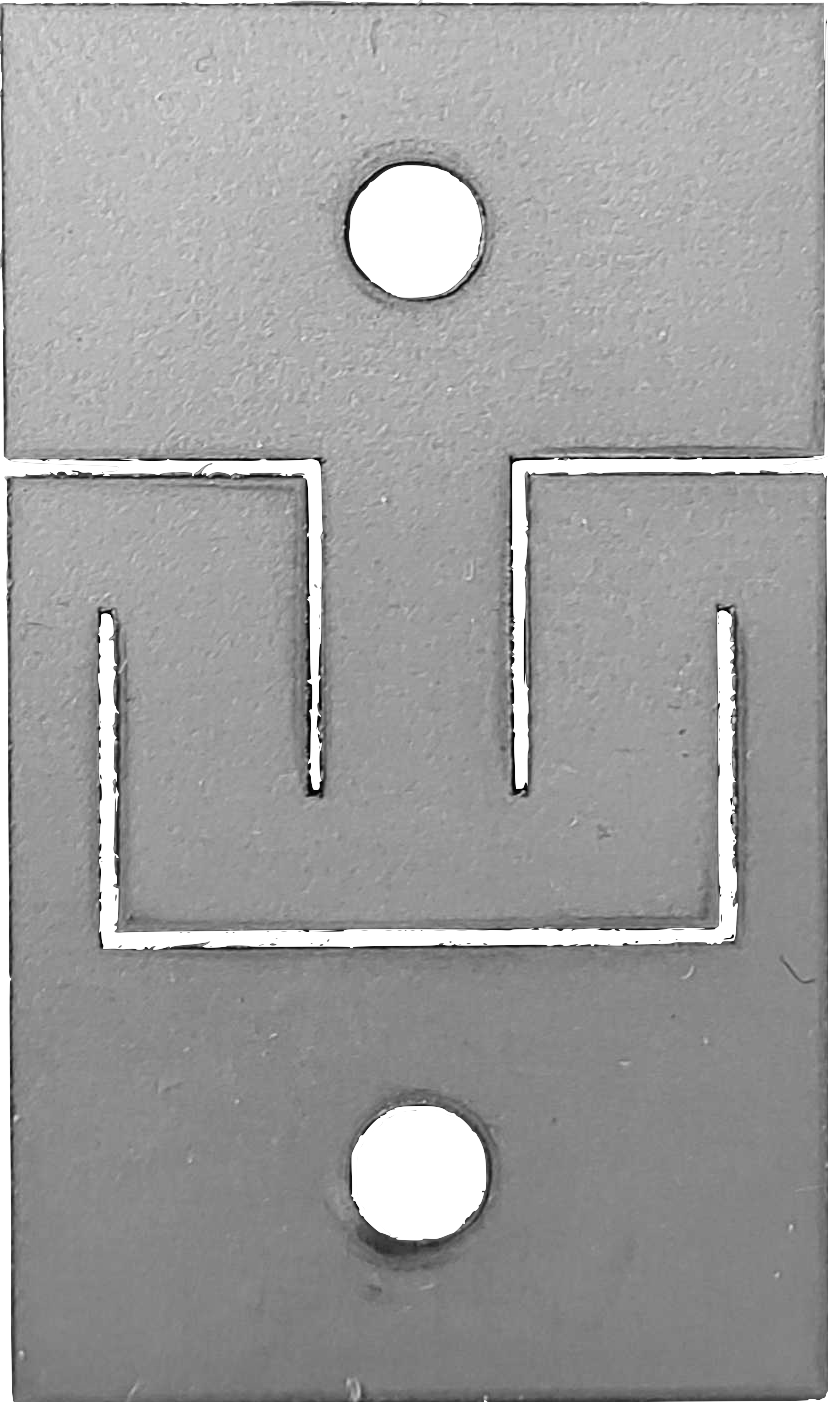
\includegraphics[width = 1.25cm]{images/chap5/sma-kiri-unit-grey.png}
        };

        \node[anchor=north west,inner sep=0] (graph2x1) at (1.05,0.43) {
            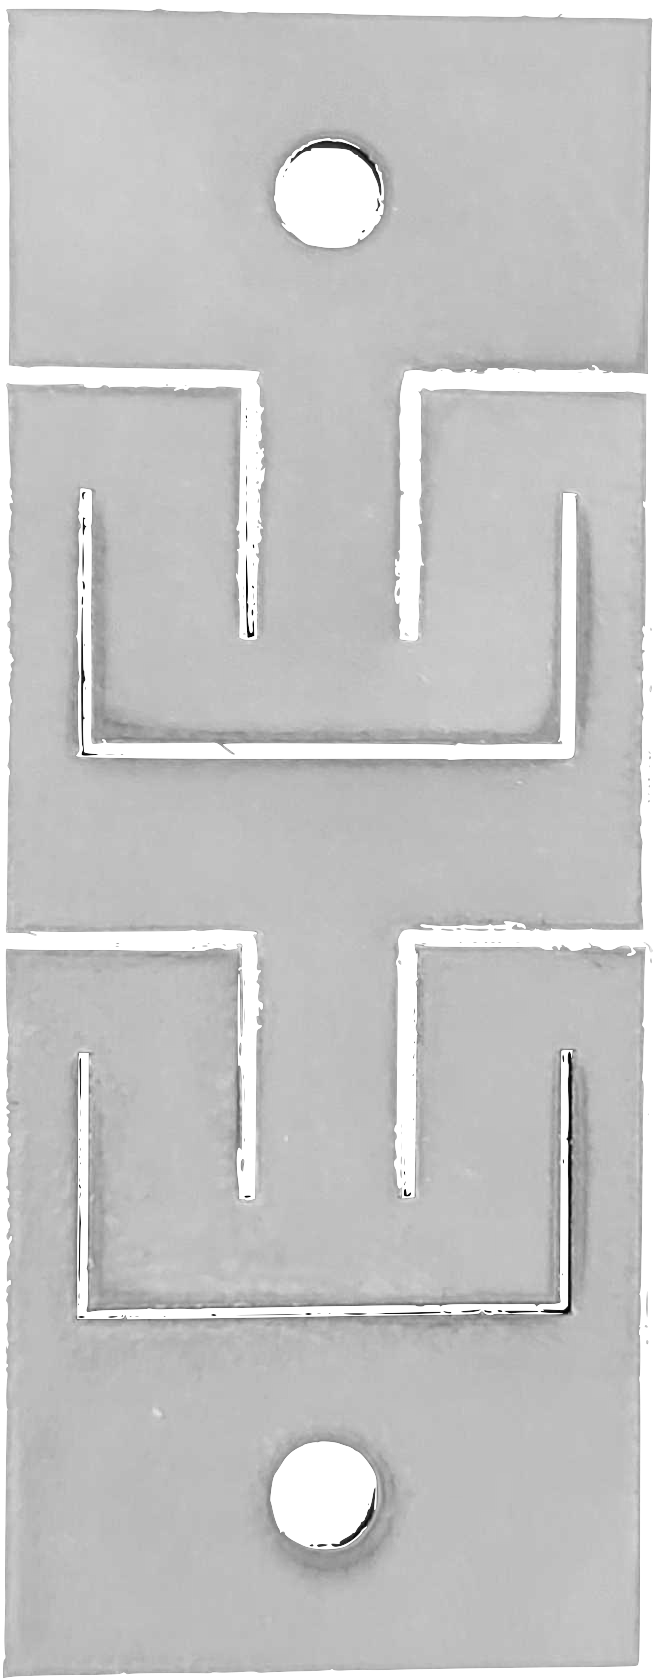
\includegraphics[width = 1.25cm]{images/chap5/sma-kiri-2x1.png}
        };

        \node[anchor=north west,inner sep=0] (graph1x2) at (1.00,1.0) {
            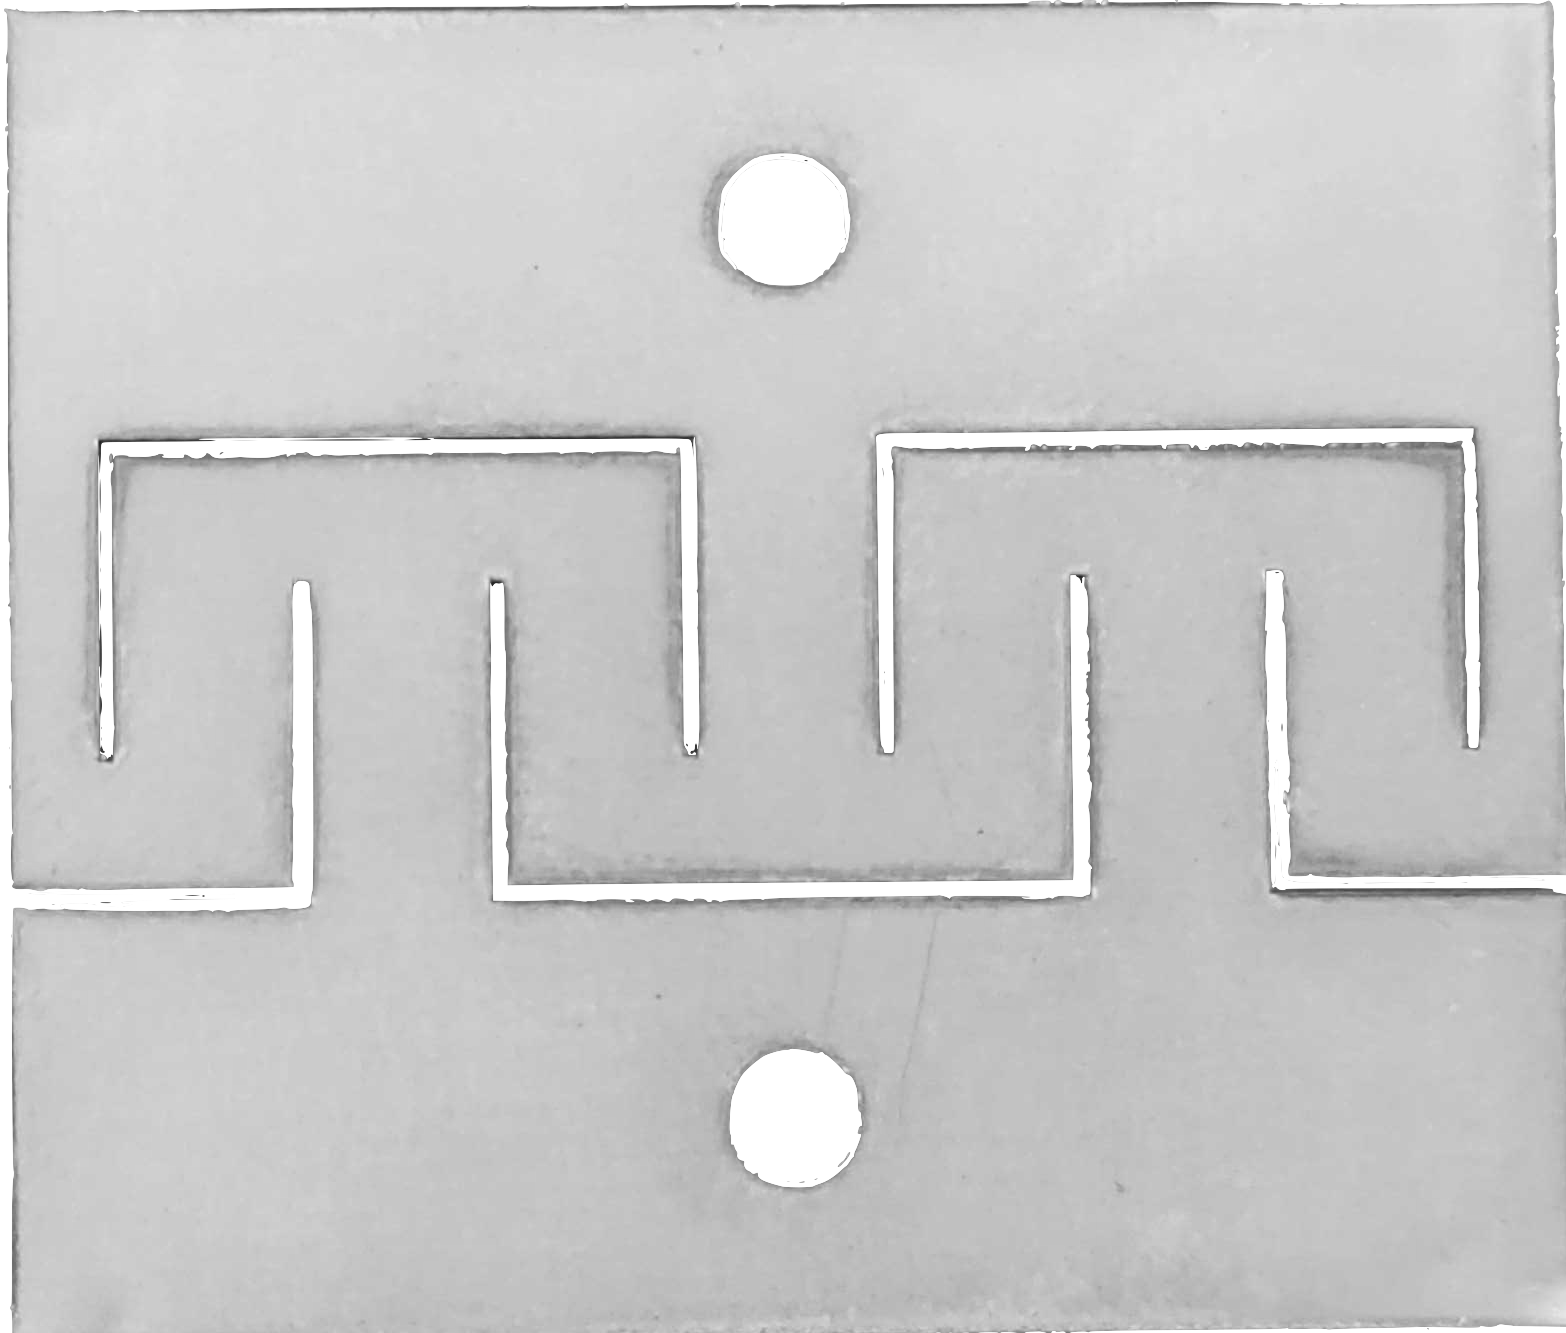
\includegraphics[width = 2.5cm]{images/chap5/sma-kiri-1x2.png}
        };
      % \draw[help lines,xstep=.05,ystep=.05] (0,0) grid (1,1);
      %   \foreach \x in {0,1,...,9} { \node [anchor=north] at (\x/10,0) {0.\x}; }
      %   \foreach \y in {0,1,...,9} { \node [anchor=east] at (0,\y/10) {0.\y}; }
    \end{scope}
    \draw[lightcolor, ultra thick] (graph1x1.south east) rectangle (graph1x1.north west);
    \draw[middlecolor, ultra thick] (graph2x1.south east) rectangle (graph2x1.north west);
    \draw[darkcolor, ultra thick] (graph1x2.south east) rectangle (graph1x2.north west);



\end{tikzpicture}
\end{document}
